% A_fi.tex -- online appendix: variable importance details (2026-10-26, integration and pruning pass, JFEc page
% budget; writeup/INTEGRATION_SPEC_2026-10-26.md, VI agent). Material moved out of the main-text section Variable
% importance (rehaul/08_feature_importance.tex, label sec:rh_fi), lightly edited: the construction and its checks, the
% rankings and their time profile, the conditional shares, the response shapes and interactions, the window test
% (P1/P2) and the trees across windows, and the window x feature-count grid (framing B of
% writeup/drafts/2026-10-26_complexity.tex only: data and feature scaling; the complexity framing in the sense of
% KellyMalamudZhou2024 is not used, per the spec). Floats moved with their text: tab:rh_fip_nonstd, fig:rh_fip_rank,
% fig:rh_fip_time, fig:rh_fip_cond (from 08_feature_importance_floats.tex); tab:rh_fip_window, tab:rh_fip_lc,
% tab:rh_fip_inter, fig:rh_fip_shapes (from 08b_fi_measures_floats.tex); fig:rh_cx_complexity, fig:rh_cx_scaling
% (generated/rehaul_complexity_floats.tex). Macros: \rhfip... (generated/rehaul_fip_numbers.tex), \rhlc...
% (generated/rehaul_fip_lc_numbers.tex), \rhcx... (generated/rehaul_complexity_numbers.tex), \rhor...
% (generated/rehaul_oos_rerun_numbers.tex); all loaded in the preamble of paper_rehaul.tex (FRONT adds
% rehaul_complexity_numbers). The file holds \subsection's only; APPENDIX wires it into the online appendix.
% Design note: the SHAP values, the ladder and the grid are on the design before the FOMC patch (D13); to be rerun on
% the patched design.
\ifdefined\rhfipNOrigins\else% AUTO-GENERATED by writeup/make_rehaul_fi_pooled.py -- do not edit; re-run the script.
\providecommand{\ser}[2]{#2}\providecommand{\serx}[3]{#3}
% \rhfip... macros for writeup/rehaul/08_feature_importance.tex (results/tree_shap_w3000_2014start_fomcfix_2026-10-26, the
% FOMC-patched design, its linear reference inputs/fiw_gamma_fomcfix.npz; the window study's ...W... macros:
% results/fi_by_window_2014start_2026-10-22, pre-patch; the final pooled runs, W = 3,000 trading days).
\providecommand{\rhfipNOrigins}{}\renewcommand{\rhfipNOrigins}{126}  % monthly origins (re-estimations explained)
\providecommand{\rhfipNRows}{}\renewcommand{\rhfipNRows}{33{,}970}  % bars explained, every bar of the evaluation span
\providecommand{\rhfipOriginEvery}{}\renewcommand{\rhfipOriginEvery}{21}  % trading days between origins
\providecommand{\rhfipLastBlock}{}\renewcommand{\rhfipLastBlock}{18}  % trading days of the last origin's block
\providecommand{\rhfipFirstOrigin}{}\renewcommand{\rhfipFirstOrigin}{2~January~2014}  % first origin (10:00 bar)
\providecommand{\rhfipLastOrigin}{}\renewcommand{\rhfipLastOrigin}{5~April~2024}  % last origin
\providecommand{\rhfipLastDay}{}\renewcommand{\rhfipLastDay}{30~April~2024}  % day of the last bar explained
\providecommand{\rhfipWindowDays}{}\renewcommand{\rhfipWindowDays}{3{,}000}  % rolling window, trading days
\providecommand{\rhfipWindowBars}{}\renewcommand{\rhfipWindowBars}{39{,}000}  % rolling window, bars
\providecommand{\rhfipNCols}{}\renewcommand{\rhfipNCols}{564}  % predictors of the full set
\providecommand{\rhfipNGroups}{}\renewcommand{\rhfipNGroups}{48}  % predictor groups: 46 exogenous series + HAR components + calendar dummies
\providecommand{\rhfipNExog}{}\renewcommand{\rhfipNExog}{46}  % exogenous series
\providecommand{\rhfipNPerSeries}{}\renewcommand{\rhfipNPerSeries}{12}  % predictors per exogenous series: value and availability averages at six horizons
\providecommand{\rhfipNStd}{}\renewcommand{\rhfipNStd}{12}  % standard groups
\providecommand{\rhfipNNonStd}{}\renewcommand{\rhfipNNonStd}{36}  % non-standard series
\providecommand{\rhfipNStdExog}{}\renewcommand{\rhfipNStdExog}{10}  % standard exogenous series
\providecommand{\rhfipTuneLast}{}\renewcommand{\rhfipTuneLast}{31~December~2013}  % last day of the last tuning fold (fold 3)
\providecommand{\rhfipRidgePen}{}\renewcommand{\rhfipRidgePen}{\ensuremath{10^{3}}}
\providecommand{\rhfipLassoPen}{}\renewcommand{\rhfipLassoPen}{\ensuremath{10^{-4}}}
\providecommand{\rhfipEnetPen}{}\renewcommand{\rhfipEnetPen}{\ensuremath{10^{-3}}}
\providecommand{\rhfipHarPf}{}\renewcommand{\rhfipHarPf}{0.01}  % penalty factor, HAR block
\providecommand{\rhfipBootBlock}{}\renewcommand{\rhfipBootBlock}{12}  % bootstrap block, origins
\providecommand{\rhfipBootB}{}\renewcommand{\rhfipBootB}{2{,}000}
\providecommand{\rhfipCiLevel}{}\renewcommand{\rhfipCiLevel}{95}  % percentile intervals of both rules (RULE_shap.txt, RULE_fiw.txt)
\providecommand{\rhfipShapeMin}{}\renewcommand{\rhfipShapeMin}{0.5}  % M3 selection: share of at least this many percent
\providecommand{\rhfipTopN}{}\renewcommand{\rhfipTopN}{10}  % length of the top lists compared (m2_rank.csv top10_overlap)
\providecommand{\rhfipSlopeUnit}{}\renewcommand{\rhfipSlopeUnit}{1{,}000}  % trading days per unit of the window slope
\providecommand{\rhfipNMom}{}\renewcommand{\rhfipNMom}{seven}  % the futures' realized moments (standard)
\providecommand{\rhfipLgbmGateEq}{}\renewcommand{\rhfipLgbmGateEq}{126}  % origins bit-equal to the merged every-bar walk
\providecommand{\rhfipXgbGateEq}{}\renewcommand{\rhfipXgbGateEq}{126}  % origins bit-equal to the merged every-bar walk
\providecommand{\rhfipRfGateEq}{}\renewcommand{\rhfipRfGateEq}{126}  % origins bit-equal to the merged every-bar walk
\providecommand{\rhfipRfGateAtShap}{}\renewcommand{\rhfipRfGateAtShap}{126}  % forest origins the walk had written when the SHAP gate ran
\providecommand{\rhfipXgbAddMax}{}\renewcommand{\rhfipXgbAddMax}{\ensuremath{3.7\times 10^{-6}}}  % XGBoost additivity, float32
\providecommand{\rhfipXgbAddTol}{}\renewcommand{\rhfipXgbAddTol}{\ensuremath{10^{-5}}}
\providecommand{\rhfipAddMaxDouble}{}\renewcommand{\rhfipAddMaxDouble}{\ensuremath{5.1\times 10^{-14}}}
\providecommand{\rhfipLinGateMax}{}\renewcommand{\rhfipLinGateMax}{\ensuremath{4.4\times 10^{-16}}}  % linear replay vs walk forecasts, W = 3,000
\providecommand{\rhfipInterRows}{}\renewcommand{\rhfipInterRows}{1{,}008}  % M5 rows
\providecommand{\rhfipInterPerOrigin}{}\renewcommand{\rhfipInterPerOrigin}{8}  % M5 rows per origin
\providecommand{\rhfipFomcRows}{}\renewcommand{\rhfipFomcRows}{1{,}014}
\providecommand{\rhfipFomcDaysShap}{}\renewcommand{\rhfipFomcDaysShap}{78}  % FOMC statement days in the SHAP subset (M4; releases.parquet only)
\providecommand{\rhfipFomcDays}{}\renewcommand{\rhfipFomcDays}{81}  % scheduled FOMC statement days in the span (loader calendar)
\providecommand{\rhfipFomcDaysMissing}{}\renewcommand{\rhfipFomcDaysMissing}{3}  % statement days the SHAP subset leaves out (counted with the other days; the patched rerun's reducer keeps releases.parquet's days)
\providecommand{\rhfipNHolSessions}{}\renewcommand{\rhfipNHolSessions}{64}  % NYSE-holiday futures sessions among the explained bars (not scored in Table 1)
\providecommand{\rhfipNHolBars}{}\renewcommand{\rhfipNHolBars}{443}  % their regular-hours bars
\providecommand{\rhfipVixLo}{}\renewcommand{\rhfipVixLo}{13.96}
\providecommand{\rhfipVixHi}{}\renewcommand{\rhfipVixHi}{19.02}
\providecommand{\rhfipLgbmHar}{}\renewcommand{\rhfipLgbmHar}{51.7}
\providecommand{\rhfipLgbmHarLo}{}\renewcommand{\rhfipLgbmHarLo}{49.5}
\providecommand{\rhfipLgbmHarHi}{}\renewcommand{\rhfipLgbmHarHi}{53.7}
\providecommand{\rhfipLgbmMom}{}\renewcommand{\rhfipLgbmMom}{22.3}
\providecommand{\rhfipLgbmNs}{}\renewcommand{\rhfipLgbmNs}{21.8}
\providecommand{\rhfipLgbmNsLo}{}\renewcommand{\rhfipLgbmNsLo}{20.4}
\providecommand{\rhfipLgbmNsHi}{}\renewcommand{\rhfipLgbmNsHi}{23.4}
\providecommand{\rhfipLgbmNsEx}{}\renewcommand{\rhfipLgbmNsEx}{45.9}
\providecommand{\rhfipLgbmNsExLo}{}\renewcommand{\rhfipLgbmNsExLo}{44.2}
\providecommand{\rhfipLgbmNsExHi}{}\renewcommand{\rhfipLgbmNsExHi}{47.7}
\providecommand{\rhfipXgbHar}{}\renewcommand{\rhfipXgbHar}{52.0}
\providecommand{\rhfipXgbHarLo}{}\renewcommand{\rhfipXgbHarLo}{50.0}
\providecommand{\rhfipXgbHarHi}{}\renewcommand{\rhfipXgbHarHi}{53.8}
\providecommand{\rhfipXgbMom}{}\renewcommand{\rhfipXgbMom}{23.6}
\providecommand{\rhfipXgbNs}{}\renewcommand{\rhfipXgbNs}{20.6}
\providecommand{\rhfipXgbNsLo}{}\renewcommand{\rhfipXgbNsLo}{19.2}
\providecommand{\rhfipXgbNsHi}{}\renewcommand{\rhfipXgbNsHi}{22.2}
\providecommand{\rhfipXgbNsEx}{}\renewcommand{\rhfipXgbNsEx}{43.6}
\providecommand{\rhfipXgbNsExLo}{}\renewcommand{\rhfipXgbNsExLo}{41.8}
\providecommand{\rhfipXgbNsExHi}{}\renewcommand{\rhfipXgbNsExHi}{45.7}
\providecommand{\rhfipRfHar}{}\renewcommand{\rhfipRfHar}{57.6}
\providecommand{\rhfipRfHarLo}{}\renewcommand{\rhfipRfHarLo}{55.4}
\providecommand{\rhfipRfHarHi}{}\renewcommand{\rhfipRfHarHi}{59.6}
\providecommand{\rhfipRfMom}{}\renewcommand{\rhfipRfMom}{20.7}
\providecommand{\rhfipRfNs}{}\renewcommand{\rhfipRfNs}{18.6}
\providecommand{\rhfipRfNsLo}{}\renewcommand{\rhfipRfNsLo}{17.2}
\providecommand{\rhfipRfNsHi}{}\renewcommand{\rhfipRfNsHi}{20.3}
\providecommand{\rhfipRfNsEx}{}\renewcommand{\rhfipRfNsEx}{44.2}
\providecommand{\rhfipRfNsExLo}{}\renewcommand{\rhfipRfNsExLo}{42.1}
\providecommand{\rhfipRfNsExHi}{}\renewcommand{\rhfipRfNsExHi}{46.5}
\providecommand{\rhfipRidgeNsEx}{}\renewcommand{\rhfipRidgeNsEx}{68.8}
\providecommand{\rhfipRidgeNs}{}\renewcommand{\rhfipRidgeNs}{55.6}
\providecommand{\rhfipRidgeHar}{}\renewcommand{\rhfipRidgeHar}{17.5}
\providecommand{\rhfipLassoNsEx}{}\renewcommand{\rhfipLassoNsEx}{82.5}
\providecommand{\rhfipLassoNs}{}\renewcommand{\rhfipLassoNs}{76.5}
\providecommand{\rhfipLassoHar}{}\renewcommand{\rhfipLassoHar}{6.7}
\providecommand{\rhfipEnetNsEx}{}\renewcommand{\rhfipEnetNsEx}{60.0}
\providecommand{\rhfipEnetNs}{}\renewcommand{\rhfipEnetNs}{42.9}
\providecommand{\rhfipEnetHar}{}\renewcommand{\rhfipEnetHar}{26.4}
\providecommand{\rhfipHarMin}{}\renewcommand{\rhfipHarMin}{51.7}
\providecommand{\rhfipHarMax}{}\renewcommand{\rhfipHarMax}{57.6}
\providecommand{\rhfipMomMin}{}\renewcommand{\rhfipMomMin}{20.7}
\providecommand{\rhfipMomMax}{}\renewcommand{\rhfipMomMax}{23.6}
\providecommand{\rhfipNsExMin}{}\renewcommand{\rhfipNsExMin}{43.6}
\providecommand{\rhfipNsExMax}{}\renewcommand{\rhfipNsExMax}{45.9}
\providecommand{\rhfipSentMin}{}\renewcommand{\rhfipSentMin}{0.6}
\providecommand{\rhfipSentMax}{}\renewcommand{\rhfipSentMax}{0.8}
\providecommand{\rhfipVdMin}{}\renewcommand{\rhfipVdMin}{0.2}
\providecommand{\rhfipVdMax}{}\renewcommand{\rhfipVdMax}{0.3}
\providecommand{\rhfipFomcBucketMin}{}\renewcommand{\rhfipFomcBucketMin}{1.4}
\providecommand{\rhfipFomcBucketMax}{}\renewcommand{\rhfipFomcBucketMax}{2.3}
\providecommand{\rhfipVvixMin}{}\renewcommand{\rhfipVvixMin}{0.2}
\providecommand{\rhfipVvixMax}{}\renewcommand{\rhfipVvixMax}{0.3}
\providecommand{\rhfipVixThreeMMin}{}\renewcommand{\rhfipVixThreeMMin}{0.3}
\providecommand{\rhfipVixThreeMMax}{}\renewcommand{\rhfipVixThreeMMax}{0.7}
\providecommand{\rhfipFomcDayMin}{}\renewcommand{\rhfipFomcDayMin}{0.1}
\providecommand{\rhfipFomcDayMax}{}\renewcommand{\rhfipFomcDayMax}{0.1}
\providecommand{\rhfipNsOne}{}\renewcommand{\rhfipNsOne}{\ensuremath{\ser{sumabsret_vwstock}{\mathrm{RAV}^{\mathrm{VW}}}}}
\providecommand{\rhfipNsOneMin}{}\renewcommand{\rhfipNsOneMin}{2.4}
\providecommand{\rhfipNsOneMax}{}\renewcommand{\rhfipNsOneMax}{3.9}
\providecommand{\rhfipNsOneLgbm}{}\renewcommand{\rhfipNsOneLgbm}{3.5}
\providecommand{\rhfipNsOneXgb}{}\renewcommand{\rhfipNsOneXgb}{3.9}
\providecommand{\rhfipNsOneRf}{}\renewcommand{\rhfipNsOneRf}{2.4}
\providecommand{\rhfipNsTwo}{}\renewcommand{\rhfipNsTwo}{\ensuremath{\ser{sumabsret_ewstock}{\mathrm{RAV}^{\mathrm{EW}}}}}
\providecommand{\rhfipNsTwoMin}{}\renewcommand{\rhfipNsTwoMin}{1.9}
\providecommand{\rhfipNsTwoMax}{}\renewcommand{\rhfipNsTwoMax}{3.9}
\providecommand{\rhfipNsTwoLgbm}{}\renewcommand{\rhfipNsTwoLgbm}{3.9}
\providecommand{\rhfipNsTwoXgb}{}\renewcommand{\rhfipNsTwoXgb}{3.8}
\providecommand{\rhfipNsTwoRf}{}\renewcommand{\rhfipNsTwoRf}{1.9}
\providecommand{\rhfipNsThree}{}\renewcommand{\rhfipNsThree}{\ensuremath{\ser{fomc_until_inv}{\mathrm{FOMC}^{\mathrm{next}}}}}
\providecommand{\rhfipNsThreeMin}{}\renewcommand{\rhfipNsThreeMin}{1.1}
\providecommand{\rhfipNsThreeMax}{}\renewcommand{\rhfipNsThreeMax}{2.0}
\providecommand{\rhfipNsThreeLgbm}{}\renewcommand{\rhfipNsThreeLgbm}{2.0}
\providecommand{\rhfipNsThreeXgb}{}\renewcommand{\rhfipNsThreeXgb}{2.0}
\providecommand{\rhfipNsThreeRf}{}\renewcommand{\rhfipNsThreeRf}{1.1}
\providecommand{\rhfipNsFour}{}\renewcommand{\rhfipNsFour}{\ensuremath{\ser{ofi_vwstock}{\mathrm{OFI}^{\mathrm{VW}}}}}
\providecommand{\rhfipNsFourMin}{}\renewcommand{\rhfipNsFourMin}{1.4}
\providecommand{\rhfipNsFourMax}{}\renewcommand{\rhfipNsFourMax}{1.8}
\providecommand{\rhfipNsFourLgbm}{}\renewcommand{\rhfipNsFourLgbm}{1.8}
\providecommand{\rhfipNsFourXgb}{}\renewcommand{\rhfipNsFourXgb}{1.7}
\providecommand{\rhfipNsFourRf}{}\renewcommand{\rhfipNsFourRf}{1.4}
\providecommand{\rhfipNsFive}{}\renewcommand{\rhfipNsFive}{\ensuremath{\ser{effspread_vwstock}{\mathrm{EffSpread}^{\mathrm{VW}}}}}
\providecommand{\rhfipNsFiveMin}{}\renewcommand{\rhfipNsFiveMin}{1.2}
\providecommand{\rhfipNsFiveMax}{}\renewcommand{\rhfipNsFiveMax}{1.3}
\providecommand{\rhfipNsFiveLgbm}{}\renewcommand{\rhfipNsFiveLgbm}{1.2}
\providecommand{\rhfipNsFiveXgb}{}\renewcommand{\rhfipNsFiveXgb}{1.2}
\providecommand{\rhfipNsFiveRf}{}\renewcommand{\rhfipNsFiveRf}{1.3}
\providecommand{\rhfipTreeTopOne}{}\renewcommand{\rhfipTreeTopOne}{\ensuremath{\ser{sumabsret}{\mathrm{RAV}}}}
\providecommand{\rhfipTreeTopTwo}{}\renewcommand{\rhfipTreeTopTwo}{\ensuremath{\ser{sumret}{r}}}
\providecommand{\rhfipLgbmTopOneEx}{}\renewcommand{\rhfipLgbmTopOneEx}{20.3}
\providecommand{\rhfipXgbTopOneEx}{}\renewcommand{\rhfipXgbTopOneEx}{24.7}
\providecommand{\rhfipRfTopOneEx}{}\renewcommand{\rhfipRfTopOneEx}{29.2}
\providecommand{\rhfipRidgeTopOne}{}\renewcommand{\rhfipRidgeTopOne}{\ensuremath{\ser{fomc_until_inv}{\mathrm{FOMC}^{\mathrm{next}}}}}
\providecommand{\rhfipRidgeTopOneEx}{}\renewcommand{\rhfipRidgeTopOneEx}{9.0}
\providecommand{\rhfipLgbmNUsedAll}{}\renewcommand{\rhfipLgbmNUsedAll}{42}  % exogenous series split on at every origin
\providecommand{\rhfipLgbmUsedMin}{}\renewcommand{\rhfipLgbmUsedMin}{58}
\providecommand{\rhfipXgbNUsedAll}{}\renewcommand{\rhfipXgbNUsedAll}{43}  % exogenous series split on at every origin
\providecommand{\rhfipXgbUsedMin}{}\renewcommand{\rhfipXgbUsedMin}{72}
\providecommand{\rhfipRfNUsedAll}{}\renewcommand{\rhfipRfNUsedAll}{46}  % exogenous series split on at every origin
\providecommand{\rhfipRfUsedMin}{}\renewcommand{\rhfipRfUsedMin}{126}
\providecommand{\rhfipLgbmDRidge}{}\renewcommand{\rhfipLgbmDRidge}{\ensuremath{-}22.9}
\providecommand{\rhfipLgbmDRidgeLo}{}\renewcommand{\rhfipLgbmDRidgeLo}{\ensuremath{-}24.8}
\providecommand{\rhfipLgbmDRidgeHi}{}\renewcommand{\rhfipLgbmDRidgeHi}{\ensuremath{-}21.1}
\providecommand{\rhfipLgbmDLasso}{}\renewcommand{\rhfipLgbmDLasso}{\ensuremath{-}36.6}
\providecommand{\rhfipLgbmDLassoLo}{}\renewcommand{\rhfipLgbmDLassoLo}{\ensuremath{-}39.1}
\providecommand{\rhfipLgbmDLassoHi}{}\renewcommand{\rhfipLgbmDLassoHi}{\ensuremath{-}34.4}
\providecommand{\rhfipLgbmDEnet}{}\renewcommand{\rhfipLgbmDEnet}{\ensuremath{-}14.1}
\providecommand{\rhfipLgbmDEnetLo}{}\renewcommand{\rhfipLgbmDEnetLo}{\ensuremath{-}15.7}
\providecommand{\rhfipLgbmDEnetHi}{}\renewcommand{\rhfipLgbmDEnetHi}{\ensuremath{-}12.7}
\providecommand{\rhfipXgbDRidge}{}\renewcommand{\rhfipXgbDRidge}{\ensuremath{-}25.1}
\providecommand{\rhfipXgbDRidgeLo}{}\renewcommand{\rhfipXgbDRidgeLo}{\ensuremath{-}27.0}
\providecommand{\rhfipXgbDRidgeHi}{}\renewcommand{\rhfipXgbDRidgeHi}{\ensuremath{-}23.3}
\providecommand{\rhfipXgbDLasso}{}\renewcommand{\rhfipXgbDLasso}{\ensuremath{-}38.9}
\providecommand{\rhfipXgbDLassoLo}{}\renewcommand{\rhfipXgbDLassoLo}{\ensuremath{-}41.4}
\providecommand{\rhfipXgbDLassoHi}{}\renewcommand{\rhfipXgbDLassoHi}{\ensuremath{-}36.6}
\providecommand{\rhfipXgbDEnet}{}\renewcommand{\rhfipXgbDEnet}{\ensuremath{-}16.3}
\providecommand{\rhfipXgbDEnetLo}{}\renewcommand{\rhfipXgbDEnetLo}{\ensuremath{-}17.8}
\providecommand{\rhfipXgbDEnetHi}{}\renewcommand{\rhfipXgbDEnetHi}{\ensuremath{-}14.9}
\providecommand{\rhfipRfDRidge}{}\renewcommand{\rhfipRfDRidge}{\ensuremath{-}24.5}
\providecommand{\rhfipRfDRidgeLo}{}\renewcommand{\rhfipRfDRidgeLo}{\ensuremath{-}26.3}
\providecommand{\rhfipRfDRidgeHi}{}\renewcommand{\rhfipRfDRidgeHi}{\ensuremath{-}22.9}
\providecommand{\rhfipRfDLasso}{}\renewcommand{\rhfipRfDLasso}{\ensuremath{-}38.3}
\providecommand{\rhfipRfDLassoLo}{}\renewcommand{\rhfipRfDLassoLo}{\ensuremath{-}40.5}
\providecommand{\rhfipRfDLassoHi}{}\renewcommand{\rhfipRfDLassoHi}{\ensuremath{-}36.3}
\providecommand{\rhfipRfDEnet}{}\renewcommand{\rhfipRfDEnet}{\ensuremath{-}15.7}
\providecommand{\rhfipRfDEnetLo}{}\renewcommand{\rhfipRfDEnetLo}{\ensuremath{-}17.0}
\providecommand{\rhfipRfDEnetHi}{}\renewcommand{\rhfipRfDEnetHi}{\ensuremath{-}14.4}
\providecommand{\rhfipNDLess}{}\renewcommand{\rhfipNDLess}{27}  % tree-minus-linear D with the 95% interval below 0
\providecommand{\rhfipNDAll}{}\renewcommand{\rhfipNDAll}{27}  % D comparisons: 3 trees x 3 linear models x 3 denominators
\providecommand{\rhfipLgbmSpRidge}{}\renewcommand{\rhfipLgbmSpRidge}{0.57}
\providecommand{\rhfipLgbmTopRidge}{}\renewcommand{\rhfipLgbmTopRidge}{6}
\providecommand{\rhfipLgbmSpLasso}{}\renewcommand{\rhfipLgbmSpLasso}{0.49}
\providecommand{\rhfipLgbmTopLasso}{}\renewcommand{\rhfipLgbmTopLasso}{5}
\providecommand{\rhfipLgbmSpEnet}{}\renewcommand{\rhfipLgbmSpEnet}{0.66}
\providecommand{\rhfipLgbmTopEnet}{}\renewcommand{\rhfipLgbmTopEnet}{6}
\providecommand{\rhfipXgbSpRidge}{}\renewcommand{\rhfipXgbSpRidge}{0.55}
\providecommand{\rhfipXgbTopRidge}{}\renewcommand{\rhfipXgbTopRidge}{6}
\providecommand{\rhfipXgbSpLasso}{}\renewcommand{\rhfipXgbSpLasso}{0.47}
\providecommand{\rhfipXgbTopLasso}{}\renewcommand{\rhfipXgbTopLasso}{5}
\providecommand{\rhfipXgbSpEnet}{}\renewcommand{\rhfipXgbSpEnet}{0.63}
\providecommand{\rhfipXgbTopEnet}{}\renewcommand{\rhfipXgbTopEnet}{6}
\providecommand{\rhfipRfSpRidge}{}\renewcommand{\rhfipRfSpRidge}{0.53}
\providecommand{\rhfipRfTopRidge}{}\renewcommand{\rhfipRfTopRidge}{5}
\providecommand{\rhfipRfSpLasso}{}\renewcommand{\rhfipRfSpLasso}{0.43}
\providecommand{\rhfipRfTopLasso}{}\renewcommand{\rhfipRfTopLasso}{4}
\providecommand{\rhfipRfSpEnet}{}\renewcommand{\rhfipRfSpEnet}{0.60}
\providecommand{\rhfipRfTopEnet}{}\renewcommand{\rhfipRfTopEnet}{5}
\providecommand{\rhfipSpLgbmXgb}{}\renewcommand{\rhfipSpLgbmXgb}{0.99}
\providecommand{\rhfipSpLgbmRf}{}\renewcommand{\rhfipSpLgbmRf}{0.90}
\providecommand{\rhfipSpXgbRf}{}\renewcommand{\rhfipSpXgbRf}{0.89}
\providecommand{\rhfipRidgeRankFomcUntil}{}\renewcommand{\rhfipRidgeRankFomcUntil}{1}
\providecommand{\rhfipTreeRankFomcUntilMin}{}\renewcommand{\rhfipTreeRankFomcUntilMin}{6}
\providecommand{\rhfipTreeRankFomcUntilMax}{}\renewcommand{\rhfipTreeRankFomcUntilMax}{10}
\providecommand{\rhfipRidgeRankFomcDay}{}\renewcommand{\rhfipRidgeRankFomcDay}{9}
\providecommand{\rhfipTreeRankFomcDayMin}{}\renewcommand{\rhfipTreeRankFomcDayMin}{39}
\providecommand{\rhfipTreeRankFomcDayMax}{}\renewcommand{\rhfipTreeRankFomcDayMax}{43}
\providecommand{\rhfipFomcUntil}{}\renewcommand{\rhfipFomcUntil}{\ensuremath{\ser{fomc_until_inv}{\mathrm{FOMC}^{\mathrm{next}}}}}
\providecommand{\rhfipFomcDay}{}\renewcommand{\rhfipFomcDay}{\ensuremath{\ser{fomc_day}{\mathrm{FOMC}^{\mathrm{day}}}}}
\providecommand{\rhfipAbsVw}{}\renewcommand{\rhfipAbsVw}{\ensuremath{\ser{sumabsret_vwstock}{\mathrm{RAV}^{\mathrm{VW}}}}}
\providecommand{\rhfipOfi}{}\renewcommand{\rhfipOfi}{\ensuremath{\ser{ofi_vwstock}{\mathrm{OFI}^{\mathrm{VW}}}}}
\providecommand{\rhfipLgbmNeff}{}\renewcommand{\rhfipLgbmNeff}{11.0}
\providecommand{\rhfipLgbmNHalf}{}\renewcommand{\rhfipLgbmNHalf}{4}
\providecommand{\rhfipLgbmNEighty}{}\renewcommand{\rhfipLgbmNEighty}{13}
\providecommand{\rhfipXgbNeff}{}\renewcommand{\rhfipXgbNeff}{9.1}
\providecommand{\rhfipXgbNHalf}{}\renewcommand{\rhfipXgbNHalf}{4}
\providecommand{\rhfipXgbNEighty}{}\renewcommand{\rhfipXgbNEighty}{11}
\providecommand{\rhfipRfNeff}{}\renewcommand{\rhfipRfNeff}{8.9}
\providecommand{\rhfipRfNHalf}{}\renewcommand{\rhfipRfNHalf}{4}
\providecommand{\rhfipRfNEighty}{}\renewcommand{\rhfipRfNEighty}{16}
\providecommand{\rhfipRidgeNeff}{}\renewcommand{\rhfipRidgeNeff}{28.5}
\providecommand{\rhfipRidgeNHalf}{}\renewcommand{\rhfipRidgeNHalf}{11}
\providecommand{\rhfipRidgeNEighty}{}\renewcommand{\rhfipRidgeNEighty}{26}
\providecommand{\rhfipLassoNeff}{}\renewcommand{\rhfipLassoNeff}{5.1}
\providecommand{\rhfipLassoNHalf}{}\renewcommand{\rhfipLassoNHalf}{2}
\providecommand{\rhfipLassoNEighty}{}\renewcommand{\rhfipLassoNEighty}{11}
\providecommand{\rhfipEnetNeff}{}\renewcommand{\rhfipEnetNeff}{16.2}
\providecommand{\rhfipEnetNHalf}{}\renewcommand{\rhfipEnetNHalf}{6}
\providecommand{\rhfipEnetNEighty}{}\renewcommand{\rhfipEnetNEighty}{15}
\providecommand{\rhfipYearFirst}{}\renewcommand{\rhfipYearFirst}{2014}
\providecommand{\rhfipYearLast}{}\renewcommand{\rhfipYearLast}{2024}
\providecommand{\rhfipLgbmNsYearMin}{}\renewcommand{\rhfipLgbmNsYearMin}{18.1}
\providecommand{\rhfipLgbmNsYearMinYr}{}\renewcommand{\rhfipLgbmNsYearMinYr}{2021}
\providecommand{\rhfipLgbmNsYearMax}{}\renewcommand{\rhfipLgbmNsYearMax}{25.6}
\providecommand{\rhfipLgbmNsYearMaxYr}{}\renewcommand{\rhfipLgbmNsYearMaxYr}{2015}
\providecommand{\rhfipLgbmHarYearMax}{}\renewcommand{\rhfipLgbmHarYearMax}{57.4}
\providecommand{\rhfipLgbmHarYearMaxYr}{}\renewcommand{\rhfipLgbmHarYearMaxYr}{2021}
\providecommand{\rhfipLgbmHarYearMin}{}\renewcommand{\rhfipLgbmHarYearMin}{44.6}
\providecommand{\rhfipLgbmHarYearMinYr}{}\renewcommand{\rhfipLgbmHarYearMinYr}{2017}
\providecommand{\rhfipXgbNsYearMin}{}\renewcommand{\rhfipXgbNsYearMin}{17.2}
\providecommand{\rhfipXgbNsYearMinYr}{}\renewcommand{\rhfipXgbNsYearMinYr}{2021}
\providecommand{\rhfipXgbNsYearMax}{}\renewcommand{\rhfipXgbNsYearMax}{24.3}
\providecommand{\rhfipXgbNsYearMaxYr}{}\renewcommand{\rhfipXgbNsYearMaxYr}{2015}
\providecommand{\rhfipXgbHarYearMax}{}\renewcommand{\rhfipXgbHarYearMax}{57.0}
\providecommand{\rhfipXgbHarYearMaxYr}{}\renewcommand{\rhfipXgbHarYearMaxYr}{2021}
\providecommand{\rhfipXgbHarYearMin}{}\renewcommand{\rhfipXgbHarYearMin}{45.8}
\providecommand{\rhfipXgbHarYearMinYr}{}\renewcommand{\rhfipXgbHarYearMinYr}{2017}
\providecommand{\rhfipRfNsYearMin}{}\renewcommand{\rhfipRfNsYearMin}{15.2}
\providecommand{\rhfipRfNsYearMinYr}{}\renewcommand{\rhfipRfNsYearMinYr}{2021}
\providecommand{\rhfipRfNsYearMax}{}\renewcommand{\rhfipRfNsYearMax}{22.9}
\providecommand{\rhfipRfNsYearMaxYr}{}\renewcommand{\rhfipRfNsYearMaxYr}{2015}
\providecommand{\rhfipRfHarYearMax}{}\renewcommand{\rhfipRfHarYearMax}{62.3}
\providecommand{\rhfipRfHarYearMaxYr}{}\renewcommand{\rhfipRfHarYearMaxYr}{2019}
\providecommand{\rhfipRfHarYearMin}{}\renewcommand{\rhfipRfHarYearMin}{50.4}
\providecommand{\rhfipRfHarYearMinYr}{}\renewcommand{\rhfipRfHarYearMinYr}{2017}
\providecommand{\rhfipNsYearMinYr}{}\renewcommand{\rhfipNsYearMinYr}{2021}  % the year of every tree's lowest non-standard share
\providecommand{\rhfipDipFirst}{}\renewcommand{\rhfipDipFirst}{2018}  % first of the years in which every tree's non-standard share is below its pooled share
\providecommand{\rhfipDipLast}{}\renewcommand{\rhfipDipLast}{2022}
\providecommand{\rhfipRidgeNsExYearMin}{}\renewcommand{\rhfipRidgeNsExYearMin}{65.1}
\providecommand{\rhfipRidgeNsExYearMinYr}{}\renewcommand{\rhfipRidgeNsExYearMinYr}{2021}
\providecommand{\rhfipRidgeNsExYearMax}{}\renewcommand{\rhfipRidgeNsExYearMax}{72.4}
\providecommand{\rhfipRidgeNsExYearMaxYr}{}\renewcommand{\rhfipRidgeNsExYearMaxYr}{2017}
\providecommand{\rhfipLassoNsExYearMin}{}\renewcommand{\rhfipLassoNsExYearMin}{77.1}
\providecommand{\rhfipLassoNsExYearMinYr}{}\renewcommand{\rhfipLassoNsExYearMinYr}{2021}
\providecommand{\rhfipLassoNsExYearMax}{}\renewcommand{\rhfipLassoNsExYearMax}{87.1}
\providecommand{\rhfipLassoNsExYearMaxYr}{}\renewcommand{\rhfipLassoNsExYearMaxYr}{2017}
\providecommand{\rhfipEnetNsExYearMin}{}\renewcommand{\rhfipEnetNsExYearMin}{56.1}
\providecommand{\rhfipEnetNsExYearMinYr}{}\renewcommand{\rhfipEnetNsExYearMinYr}{2019}
\providecommand{\rhfipEnetNsExYearMax}{}\renewcommand{\rhfipEnetNsExYearMax}{65.2}
\providecommand{\rhfipEnetNsExYearMaxYr}{}\renewcommand{\rhfipEnetNsExYearMaxYr}{2014}
\providecommand{\rhfipLgbmNsExYearMin}{}\renewcommand{\rhfipLgbmNsExYearMin}{42.3}
\providecommand{\rhfipLgbmNsExYearMax}{}\renewcommand{\rhfipLgbmNsExYearMax}{50.1}
\providecommand{\rhfipXgbNsExYearMin}{}\renewcommand{\rhfipXgbNsExYearMin}{39.4}
\providecommand{\rhfipXgbNsExYearMax}{}\renewcommand{\rhfipXgbNsExYearMax}{48.9}
\providecommand{\rhfipRfNsExYearMin}{}\renewcommand{\rhfipRfNsExYearMin}{39.5}
\providecommand{\rhfipRfNsExYearMax}{}\renewcommand{\rhfipRfNsExYearMax}{50.9}
\providecommand{\rhfipLgbmNShape}{}\renewcommand{\rhfipLgbmNShape}{11}  % non-standard series at >= 0.5% (M3)
\providecommand{\rhfipLgbmNMono}{}\renewcommand{\rhfipLgbmNMono}{7}
\providecommand{\rhfipLgbmNIrr}{}\renewcommand{\rhfipLgbmNIrr}{3}
\providecommand{\rhfipLgbmNStep}{}\renewcommand{\rhfipLgbmNStep}{1}
\providecommand{\rhfipLgbmNFlat}{}\renewcommand{\rhfipLgbmNFlat}{0}
\providecommand{\rhfipLgbmNThresh}{}\renewcommand{\rhfipLgbmNThresh}{0}
\providecommand{\rhfipLgbmNU}{}\renewcommand{\rhfipLgbmNU}{0}
\providecommand{\rhfipLgbmNAsym}{}\renewcommand{\rhfipLgbmNAsym}{9}
\providecommand{\rhfipXgbNShape}{}\renewcommand{\rhfipXgbNShape}{10}  % non-standard series at >= 0.5% (M3)
\providecommand{\rhfipXgbNMono}{}\renewcommand{\rhfipXgbNMono}{5}
\providecommand{\rhfipXgbNIrr}{}\renewcommand{\rhfipXgbNIrr}{3}
\providecommand{\rhfipXgbNStep}{}\renewcommand{\rhfipXgbNStep}{0}
\providecommand{\rhfipXgbNFlat}{}\renewcommand{\rhfipXgbNFlat}{1}
\providecommand{\rhfipXgbNThresh}{}\renewcommand{\rhfipXgbNThresh}{1}
\providecommand{\rhfipXgbNU}{}\renewcommand{\rhfipXgbNU}{0}
\providecommand{\rhfipXgbNAsym}{}\renewcommand{\rhfipXgbNAsym}{8}
\providecommand{\rhfipRfNShape}{}\renewcommand{\rhfipRfNShape}{13}  % non-standard series at >= 0.5% (M3)
\providecommand{\rhfipRfNMono}{}\renewcommand{\rhfipRfNMono}{10}
\providecommand{\rhfipRfNIrr}{}\renewcommand{\rhfipRfNIrr}{3}
\providecommand{\rhfipRfNStep}{}\renewcommand{\rhfipRfNStep}{0}
\providecommand{\rhfipRfNFlat}{}\renewcommand{\rhfipRfNFlat}{0}
\providecommand{\rhfipRfNThresh}{}\renewcommand{\rhfipRfNThresh}{0}
\providecommand{\rhfipRfNU}{}\renewcommand{\rhfipRfNU}{0}
\providecommand{\rhfipRfNAsym}{}\renewcommand{\rhfipRfNAsym}{13}
\providecommand{\rhfipNUThreshAll}{}\renewcommand{\rhfipNUThreshAll}{1}  % U-shaped, inverted-U or threshold profiles in any tree
\providecommand{\rhfipAbsVwLgbmLo}{}\renewcommand{\rhfipAbsVwLgbmLo}{\ensuremath{-}1.4}
\providecommand{\rhfipAbsVwLgbmHi}{}\renewcommand{\rhfipAbsVwLgbmHi}{3.9}
\providecommand{\rhfipAbsVwXgbLo}{}\renewcommand{\rhfipAbsVwXgbLo}{\ensuremath{-}1.5}
\providecommand{\rhfipAbsVwXgbHi}{}\renewcommand{\rhfipAbsVwXgbHi}{4.3}
\providecommand{\rhfipAbsVwRfLo}{}\renewcommand{\rhfipAbsVwRfLo}{\ensuremath{-}0.9}
\providecommand{\rhfipAbsVwRfHi}{}\renewcommand{\rhfipAbsVwRfHi}{2.3}
\providecommand{\rhfipOfiLgbmLo}{}\renewcommand{\rhfipOfiLgbmLo}{0.8}
\providecommand{\rhfipOfiLgbmHi}{}\renewcommand{\rhfipOfiLgbmHi}{\ensuremath{-}1.1}
\providecommand{\rhfipOfiXgbLo}{}\renewcommand{\rhfipOfiXgbLo}{0.8}
\providecommand{\rhfipOfiXgbHi}{}\renewcommand{\rhfipOfiXgbHi}{\ensuremath{-}0.9}
\providecommand{\rhfipOfiRfLo}{}\renewcommand{\rhfipOfiRfLo}{0.8}
\providecommand{\rhfipOfiRfHi}{}\renewcommand{\rhfipOfiRfHi}{\ensuremath{-}0.7}
\providecommand{\rhfipUntilLgbmLo}{}\renewcommand{\rhfipUntilLgbmLo}{\ensuremath{-}0.3}
\providecommand{\rhfipUntilLgbmHi}{}\renewcommand{\rhfipUntilLgbmHi}{2.9}
\providecommand{\rhfipUntilXgbLo}{}\renewcommand{\rhfipUntilXgbLo}{0.2}
\providecommand{\rhfipUntilXgbHi}{}\renewcommand{\rhfipUntilXgbHi}{2.4}
\providecommand{\rhfipUntilRfLo}{}\renewcommand{\rhfipUntilRfLo}{\ensuremath{-}0.0}
\providecommand{\rhfipUntilRfHi}{}\renewcommand{\rhfipUntilRfHi}{1.5}
\providecommand{\rhfipUntilHorizon}{}\renewcommand{\rhfipUntilHorizon}{25}  % horizon of fomc_until_inv's dominant column
\providecommand{\rhfipUntilHorizonXgb}{}\renewcommand{\rhfipUntilHorizonXgb}{1}  % the same in XGBoost (differs from the other trees')
\providecommand{\rhfipBarFirst}{}\renewcommand{\rhfipBarFirst}{10:00}
\providecommand{\rhfipBarLast}{}\renewcommand{\rhfipBarLast}{16:00}
\providecommand{\rhfipBarPeakA}{}\renewcommand{\rhfipBarPeakA}{14:30}
\providecommand{\rhfipBarPeakB}{}\renewcommand{\rhfipBarPeakB}{15:00}
\providecommand{\rhfipNBars}{}\renewcommand{\rhfipNBars}{13}
\providecommand{\rhfipLgbmNsFomc}{}\renewcommand{\rhfipLgbmNsFomc}{42.6}
\providecommand{\rhfipLgbmNsOther}{}\renewcommand{\rhfipLgbmNsOther}{20.9}
\providecommand{\rhfipLgbmUntilFomc}{}\renewcommand{\rhfipLgbmUntilFomc}{25.4}
\providecommand{\rhfipLgbmUntilOther}{}\renewcommand{\rhfipLgbmUntilOther}{1.06}
\providecommand{\rhfipLgbmFomcBucketFomc}{}\renewcommand{\rhfipLgbmFomcBucketFomc}{27.3}
\providecommand{\rhfipLgbmFomcBucketOther}{}\renewcommand{\rhfipLgbmFomcBucketOther}{1.3}
\providecommand{\rhfipLgbmHarFomc}{}\renewcommand{\rhfipLgbmHarFomc}{39.2}
\providecommand{\rhfipLgbmHarOther}{}\renewcommand{\rhfipLgbmHarOther}{52.2}
\providecommand{\rhfipLgbmNsFirstBar}{}\renewcommand{\rhfipLgbmNsFirstBar}{23.9}
\providecommand{\rhfipLgbmNsLastBar}{}\renewcommand{\rhfipLgbmNsLastBar}{20.5}
\providecommand{\rhfipLgbmNsAftMin}{}\renewcommand{\rhfipLgbmNsAftMin}{24.3}
\providecommand{\rhfipLgbmNsAftMax}{}\renewcommand{\rhfipLgbmNsAftMax}{25.2}
\providecommand{\rhfipLgbmNsMidMin}{}\renewcommand{\rhfipLgbmNsMidMin}{20.1}
\providecommand{\rhfipLgbmNsMidMax}{}\renewcommand{\rhfipLgbmNsMidMax}{21.9}
\providecommand{\rhfipLgbmFomcBucketAft}{}\renewcommand{\rhfipLgbmFomcBucketAft}{5.5}
\providecommand{\rhfipLgbmFomcBucketOtherBars}{}\renewcommand{\rhfipLgbmFomcBucketOtherBars}{1.4}  % median FOMC-announcement share over the other 11 bars
\providecommand{\rhfipLgbmFomcDiff}{}\renewcommand{\rhfipLgbmFomcDiff}{\ensuremath{+}21.7}
\providecommand{\rhfipLgbmFomcDiffLo}{}\renewcommand{\rhfipLgbmFomcDiffLo}{\ensuremath{+}19.3}
\providecommand{\rhfipLgbmFomcDiffHi}{}\renewcommand{\rhfipLgbmFomcDiffHi}{\ensuremath{+}24.1}
\providecommand{\rhfipLgbmLateDiff}{}\renewcommand{\rhfipLgbmLateDiff}{\ensuremath{-}3.4}
\providecommand{\rhfipLgbmLateDiffLo}{}\renewcommand{\rhfipLgbmLateDiffLo}{\ensuremath{-}4.3}
\providecommand{\rhfipLgbmLateDiffHi}{}\renewcommand{\rhfipLgbmLateDiffHi}{\ensuremath{-}2.5}
\providecommand{\rhfipLgbmVixDiff}{}\renewcommand{\rhfipLgbmVixDiff}{\ensuremath{-}3.2}
\providecommand{\rhfipLgbmVixDiffLo}{}\renewcommand{\rhfipLgbmVixDiffLo}{\ensuremath{-}5.3}
\providecommand{\rhfipLgbmVixDiffHi}{}\renewcommand{\rhfipLgbmVixDiffHi}{\ensuremath{-}1.1}
\providecommand{\rhfipLgbmVixHar}{}\renewcommand{\rhfipLgbmVixHar}{\ensuremath{+}5.1}
\providecommand{\rhfipLgbmVixHarLo}{}\renewcommand{\rhfipLgbmVixHarLo}{\ensuremath{+}1.8}
\providecommand{\rhfipLgbmVixHarHi}{}\renewcommand{\rhfipLgbmVixHarHi}{\ensuremath{+}8.4}
\providecommand{\rhfipLgbmVixDiffEx}{}\renewcommand{\rhfipLgbmVixDiffEx}{\ensuremath{-}2.3}
\providecommand{\rhfipLgbmVixDiffExLo}{}\renewcommand{\rhfipLgbmVixDiffExLo}{\ensuremath{-}4.5}
\providecommand{\rhfipLgbmVixDiffExHi}{}\renewcommand{\rhfipLgbmVixDiffExHi}{\ensuremath{-}0.2}
\providecommand{\rhfipXgbNsFomc}{}\renewcommand{\rhfipXgbNsFomc}{41.1}
\providecommand{\rhfipXgbNsOther}{}\renewcommand{\rhfipXgbNsOther}{19.7}
\providecommand{\rhfipXgbUntilFomc}{}\renewcommand{\rhfipXgbUntilFomc}{23.9}
\providecommand{\rhfipXgbUntilOther}{}\renewcommand{\rhfipXgbUntilOther}{1.10}
\providecommand{\rhfipXgbFomcBucketFomc}{}\renewcommand{\rhfipXgbFomcBucketFomc}{25.6}
\providecommand{\rhfipXgbFomcBucketOther}{}\renewcommand{\rhfipXgbFomcBucketOther}{1.3}
\providecommand{\rhfipXgbHarFomc}{}\renewcommand{\rhfipXgbHarFomc}{39.1}
\providecommand{\rhfipXgbHarOther}{}\renewcommand{\rhfipXgbHarOther}{52.5}
\providecommand{\rhfipXgbNsFirstBar}{}\renewcommand{\rhfipXgbNsFirstBar}{22.5}
\providecommand{\rhfipXgbNsLastBar}{}\renewcommand{\rhfipXgbNsLastBar}{19.5}
\providecommand{\rhfipXgbNsAftMin}{}\renewcommand{\rhfipXgbNsAftMin}{23.5}
\providecommand{\rhfipXgbNsAftMax}{}\renewcommand{\rhfipXgbNsAftMax}{23.7}
\providecommand{\rhfipXgbNsMidMin}{}\renewcommand{\rhfipXgbNsMidMin}{19.1}
\providecommand{\rhfipXgbNsMidMax}{}\renewcommand{\rhfipXgbNsMidMax}{20.4}
\providecommand{\rhfipXgbFomcBucketAft}{}\renewcommand{\rhfipXgbFomcBucketAft}{5.8}
\providecommand{\rhfipXgbFomcBucketOtherBars}{}\renewcommand{\rhfipXgbFomcBucketOtherBars}{1.3}  % median FOMC-announcement share over the other 11 bars
\providecommand{\rhfipXgbFomcDiff}{}\renewcommand{\rhfipXgbFomcDiff}{\ensuremath{+}21.4}
\providecommand{\rhfipXgbFomcDiffLo}{}\renewcommand{\rhfipXgbFomcDiffLo}{\ensuremath{+}19.3}
\providecommand{\rhfipXgbFomcDiffHi}{}\renewcommand{\rhfipXgbFomcDiffHi}{\ensuremath{+}23.5}
\providecommand{\rhfipXgbLateDiff}{}\renewcommand{\rhfipXgbLateDiff}{\ensuremath{-}3.1}
\providecommand{\rhfipXgbLateDiffLo}{}\renewcommand{\rhfipXgbLateDiffLo}{\ensuremath{-}4.0}
\providecommand{\rhfipXgbLateDiffHi}{}\renewcommand{\rhfipXgbLateDiffHi}{\ensuremath{-}2.3}
\providecommand{\rhfipXgbVixDiff}{}\renewcommand{\rhfipXgbVixDiff}{\ensuremath{-}3.0}
\providecommand{\rhfipXgbVixDiffLo}{}\renewcommand{\rhfipXgbVixDiffLo}{\ensuremath{-}5.1}
\providecommand{\rhfipXgbVixDiffHi}{}\renewcommand{\rhfipXgbVixDiffHi}{\ensuremath{-}0.9}
\providecommand{\rhfipXgbVixHar}{}\renewcommand{\rhfipXgbVixHar}{\ensuremath{+}3.9}
\providecommand{\rhfipXgbVixHarLo}{}\renewcommand{\rhfipXgbVixHarLo}{\ensuremath{+}0.4}
\providecommand{\rhfipXgbVixHarHi}{}\renewcommand{\rhfipXgbVixHarHi}{\ensuremath{+}7.2}
\providecommand{\rhfipXgbVixDiffEx}{}\renewcommand{\rhfipXgbVixDiffEx}{\ensuremath{-}3.2}
\providecommand{\rhfipXgbVixDiffExLo}{}\renewcommand{\rhfipXgbVixDiffExLo}{\ensuremath{-}5.7}
\providecommand{\rhfipXgbVixDiffExHi}{}\renewcommand{\rhfipXgbVixDiffExHi}{\ensuremath{-}0.8}
\providecommand{\rhfipRfNsFomc}{}\renewcommand{\rhfipRfNsFomc}{28.9}
\providecommand{\rhfipRfNsOther}{}\renewcommand{\rhfipRfNsOther}{18.3}
\providecommand{\rhfipRfUntilFomc}{}\renewcommand{\rhfipRfUntilFomc}{12.4}
\providecommand{\rhfipRfFomcBucketFomc}{}\renewcommand{\rhfipRfFomcBucketFomc}{13.0}
\providecommand{\rhfipRfFomcBucketOther}{}\renewcommand{\rhfipRfFomcBucketOther}{1.0}
\providecommand{\rhfipRfHarFomc}{}\renewcommand{\rhfipRfHarFomc}{50.8}
\providecommand{\rhfipRfHarOther}{}\renewcommand{\rhfipRfHarOther}{57.9}
\providecommand{\rhfipRfNsFirstBar}{}\renewcommand{\rhfipRfNsFirstBar}{20.1}
\providecommand{\rhfipRfNsLastBar}{}\renewcommand{\rhfipRfNsLastBar}{17.8}
\providecommand{\rhfipRfNsAftMin}{}\renewcommand{\rhfipRfNsAftMin}{19.5}
\providecommand{\rhfipRfNsAftMax}{}\renewcommand{\rhfipRfNsAftMax}{19.9}
\providecommand{\rhfipRfNsMidMin}{}\renewcommand{\rhfipRfNsMidMin}{17.8}
\providecommand{\rhfipRfNsMidMax}{}\renewcommand{\rhfipRfNsMidMax}{18.6}
\providecommand{\rhfipRfFomcBucketAft}{}\renewcommand{\rhfipRfFomcBucketAft}{3.1}
\providecommand{\rhfipRfFomcBucketOtherBars}{}\renewcommand{\rhfipRfFomcBucketOtherBars}{1.0}  % median FOMC-announcement share over the other 11 bars
\providecommand{\rhfipRfFomcDiff}{}\renewcommand{\rhfipRfFomcDiff}{\ensuremath{+}10.6}
\providecommand{\rhfipRfFomcDiffLo}{}\renewcommand{\rhfipRfFomcDiffLo}{\ensuremath{+}8.3}
\providecommand{\rhfipRfFomcDiffHi}{}\renewcommand{\rhfipRfFomcDiffHi}{\ensuremath{+}13.1}
\providecommand{\rhfipRfLateDiff}{}\renewcommand{\rhfipRfLateDiff}{\ensuremath{-}2.3}
\providecommand{\rhfipRfLateDiffLo}{}\renewcommand{\rhfipRfLateDiffLo}{\ensuremath{-}3.1}
\providecommand{\rhfipRfLateDiffHi}{}\renewcommand{\rhfipRfLateDiffHi}{\ensuremath{-}1.6}
\providecommand{\rhfipRfVixDiff}{}\renewcommand{\rhfipRfVixDiff}{\ensuremath{-}3.3}
\providecommand{\rhfipRfVixDiffLo}{}\renewcommand{\rhfipRfVixDiffLo}{\ensuremath{-}5.1}
\providecommand{\rhfipRfVixDiffHi}{}\renewcommand{\rhfipRfVixDiffHi}{\ensuremath{-}1.4}
\providecommand{\rhfipRfVixHar}{}\renewcommand{\rhfipRfVixHar}{\ensuremath{+}4.2}
\providecommand{\rhfipRfVixHarLo}{}\renewcommand{\rhfipRfVixHarLo}{\ensuremath{+}1.0}
\providecommand{\rhfipRfVixHarHi}{}\renewcommand{\rhfipRfVixHarHi}{\ensuremath{+}7.3}
\providecommand{\rhfipRfVixDiffEx}{}\renewcommand{\rhfipRfVixDiffEx}{\ensuremath{-}3.7}
\providecommand{\rhfipRfVixDiffExLo}{}\renewcommand{\rhfipRfVixDiffExLo}{\ensuremath{-}6.3}
\providecommand{\rhfipRfVixDiffExHi}{}\renewcommand{\rhfipRfVixDiffExHi}{\ensuremath{-}1.2}
\providecommand{\rhfipLgbmInterVar}{}\renewcommand{\rhfipLgbmInterVar}{33.1}
\providecommand{\rhfipLgbmInterCol}{}\renewcommand{\rhfipLgbmInterCol}{45.3}
\providecommand{\rhfipLgbmInterNs}{}\renewcommand{\rhfipLgbmInterNs}{49.6}
\providecommand{\rhfipLgbmInterStd}{}\renewcommand{\rhfipLgbmInterStd}{26.8}
\providecommand{\rhfipLgbmInterStdEx}{}\renewcommand{\rhfipLgbmInterStdEx}{40.2}  % descriptive: standard exogenous series only (no HAR, no calendar)
\providecommand{\rhfipLgbmInterHar}{}\renewcommand{\rhfipLgbmInterHar}{17.1}
\providecommand{\rhfipLgbmInterWeakMin}{}\renewcommand{\rhfipLgbmInterWeakMin}{54}
\providecommand{\rhfipLgbmInterWeakMax}{}\renewcommand{\rhfipLgbmInterWeakMax}{66}
\providecommand{\rhfipLgbmPairOne}{}\renewcommand{\rhfipLgbmPairOne}{1.25}
\providecommand{\rhfipLgbmPairTwo}{}\renewcommand{\rhfipLgbmPairTwo}{0.86}
\providecommand{\rhfipLgbmCellHarHar}{}\renewcommand{\rhfipLgbmCellHarHar}{48.0}
\providecommand{\rhfipXgbInterVar}{}\renewcommand{\rhfipXgbInterVar}{30.9}
\providecommand{\rhfipXgbInterCol}{}\renewcommand{\rhfipXgbInterCol}{42.5}
\providecommand{\rhfipXgbInterNs}{}\renewcommand{\rhfipXgbInterNs}{45.7}
\providecommand{\rhfipXgbInterStd}{}\renewcommand{\rhfipXgbInterStd}{26.0}
\providecommand{\rhfipXgbInterStdEx}{}\renewcommand{\rhfipXgbInterStdEx}{37.8}  % descriptive: standard exogenous series only (no HAR, no calendar)
\providecommand{\rhfipXgbInterHar}{}\renewcommand{\rhfipXgbInterHar}{17.6}
\providecommand{\rhfipXgbInterWeakMin}{}\renewcommand{\rhfipXgbInterWeakMin}{54}
\providecommand{\rhfipXgbInterWeakMax}{}\renewcommand{\rhfipXgbInterWeakMax}{63}
\providecommand{\rhfipXgbPairOne}{}\renewcommand{\rhfipXgbPairOne}{1.23}
\providecommand{\rhfipXgbPairTwo}{}\renewcommand{\rhfipXgbPairTwo}{0.83}
\providecommand{\rhfipXgbCellHarHar}{}\renewcommand{\rhfipXgbCellHarHar}{47.4}
\providecommand{\rhfipPairOneA}{}\renewcommand{\rhfipPairOneA}{HAR components}
\providecommand{\rhfipPairOneB}{}\renewcommand{\rhfipPairOneB}{\ensuremath{\ser{sumabsret_vwstock}{\mathrm{RAV}^{\mathrm{VW}}}}}
\providecommand{\rhfipPairTwoA}{}\renewcommand{\rhfipPairTwoA}{HAR components}
\providecommand{\rhfipPairTwoB}{}\renewcommand{\rhfipPairTwoB}{\ensuremath{\ser{sumabsret_ewstock}{\mathrm{RAV}^{\mathrm{EW}}}}}
\providecommand{\rhfipLgbmPairsHar}{}\renewcommand{\rhfipLgbmPairsHar}{7}
\providecommand{\rhfipXgbPairsHar}{}\renewcommand{\rhfipXgbPairsHar}{7}
\providecommand{\rhfipWMin}{}\renewcommand{\rhfipWMin}{1{,}000}
\providecommand{\rhfipWMax}{}\renewcommand{\rhfipWMax}{3{,}500}
\providecommand{\rhfipNWindows}{}\renewcommand{\rhfipNWindows}{6}
\providecommand{\rhfipSOneMeasures}{}\renewcommand{\rhfipSOneMeasures}{105}  % measure x common-penalty fits of the window study (P1 and P2)
\providecommand{\rhfipSOneRises}{}\renewcommand{\rhfipSOneRises}{0}  % ... of which rise with W
\providecommand{\rhfipSOneFalls}{}\renewcommand{\rhfipSOneFalls}{102}
\providecommand{\rhfipSOneFlat}{}\renewcommand{\rhfipSOneFlat}{3}
\providecommand{\rhfipSOneNotSupported}{}\renewcommand{\rhfipSOneNotSupported}{14}  % common-penalty verdicts NOT SUPPORTED
\providecommand{\rhfipSOneVerdicts}{}\renewcommand{\rhfipSOneVerdicts}{14}
\providecommand{\rhfipRidgeNeffWMin}{}\renewcommand{\rhfipRidgeNeffWMin}{29.2}
\providecommand{\rhfipRidgeNeffWMain}{}\renewcommand{\rhfipRidgeNeffWMain}{29.2}
\providecommand{\rhfipRidgeNeffWMax}{}\renewcommand{\rhfipRidgeNeffWMax}{28.2}
\providecommand{\rhfipRidgeNeffSlope}{}\renewcommand{\rhfipRidgeNeffSlope}{\ensuremath{-}0.10}
\providecommand{\rhfipRidgeNeffSlopeLo}{}\renewcommand{\rhfipRidgeNeffSlopeLo}{\ensuremath{-}0.25}
\providecommand{\rhfipRidgeNeffSlopeHi}{}\renewcommand{\rhfipRidgeNeffSlopeHi}{0.12}
\providecommand{\rhfipRidgeSOneLoNeffWMin}{}\renewcommand{\rhfipRidgeSOneLoNeffWMin}{33.9}
\providecommand{\rhfipRidgeSOneLoNeffWMax}{}\renewcommand{\rhfipRidgeSOneLoNeffWMax}{28.2}
\providecommand{\rhfipRidgeSOneHiNeffWMin}{}\renewcommand{\rhfipRidgeSOneHiNeffWMin}{29.2}
\providecommand{\rhfipRidgeSOneHiNeffWMax}{}\renewcommand{\rhfipRidgeSOneHiNeffWMax}{23.5}
\providecommand{\rhfipLassoSOneVWMin}{}\renewcommand{\rhfipLassoSOneVWMin}{38.7}
\providecommand{\rhfipLassoSOneVWMax}{}\renewcommand{\rhfipLassoSOneVWMax}{31.9}
\providecommand{\rhfipLassoSOneCWMin}{}\renewcommand{\rhfipLassoSOneCWMin}{213.3}
\providecommand{\rhfipLassoSOneCWMax}{}\renewcommand{\rhfipLassoSOneCWMax}{177.5}
\providecommand{\rhfipLassoWalkVWMin}{}\renewcommand{\rhfipLassoWalkVWMin}{38.8}
\providecommand{\rhfipLassoWalkVWMax}{}\renewcommand{\rhfipLassoWalkVWMax}{41.9}
\providecommand{\rhfipLassoSOneLo}{}\renewcommand{\rhfipLassoSOneLo}{\ensuremath{10^{-3}}}
\providecommand{\rhfipRidgeSOneLo}{}\renewcommand{\rhfipRidgeSOneLo}{\ensuremath{10^{3}}}
\providecommand{\rhfipRidgeSOneHi}{}\renewcommand{\rhfipRidgeSOneHi}{\ensuremath{10^{4}}}
\providecommand{\rhfipEnetPenWMin}{}\renewcommand{\rhfipEnetPenWMin}{\ensuremath{10^{-2}}}
\providecommand{\rhfipEnetPenWNext}{}\renewcommand{\rhfipEnetPenWNext}{\ensuremath{10^{-3}}}
\providecommand{\rhfipWNext}{}\renewcommand{\rhfipWNext}{1{,}500}
\providecommand{\rhfipRidgePOneWalk}{}\renewcommand{\rhfipRidgePOneWalk}{not supported}
\providecommand{\rhfipRidgePTwoWalk}{}\renewcommand{\rhfipRidgePTwoWalk}{not supported}
\providecommand{\rhfipLassoPOneWalk}{}\renewcommand{\rhfipLassoPOneWalk}{partly}
\providecommand{\rhfipLassoPTwoWalk}{}\renewcommand{\rhfipLassoPTwoWalk}{not supported}
\providecommand{\rhfipEnetPOneWalk}{}\renewcommand{\rhfipEnetPOneWalk}{supported}
\providecommand{\rhfipEnetPTwoWalk}{}\renewcommand{\rhfipEnetPTwoWalk}{supported}
\fi
\ifdefined\rhlcWMain\else% AUTO-GENERATED by writeup/make_rehaul_fip_lc.py -- do not edit; re-run the script.
% \rhlc... macros of Section 8's tree learning curve (rehaul/08_feature_importance.tex, tab:rh_fip_lc): the pooled
% trees at W = 1,000 / 2,000 / 3,000 / 3,500 trading days; names: Gap / GapT (full - HAR, x 10^3, NW t), Eg / T / P
% (extra gain x 10^3, NW t, p statement), DmFull / DmHar (DM between windows); Model Lgbm Xgb Rf; windows One Two
% Main Long (step tags OneTwo TwoMain MainLong OneMain); Bar (every bar) / Close (16:00). Counts at p < 0.05.
% Pending: none.
\providecommand{\rhPending}{\textit{pending}}
\providecommand{\rhlcWOne}{}\renewcommand{\rhlcWOne}{1{,}000}  % rolling window, trading days (13,000 bars)
\providecommand{\rhlcWTwo}{}\renewcommand{\rhlcWTwo}{2{,}000}  % rolling window, trading days (26,000 bars)
\providecommand{\rhlcWMain}{}\renewcommand{\rhlcWMain}{3{,}000}  % rolling window, trading days (39,000 bars)
\providecommand{\rhlcWLong}{}\renewcommand{\rhlcWLong}{3{,}500}  % rolling window, trading days (45,500 bars)
\providecommand{\rhlcFirstDay}{}\renewcommand{\rhlcFirstDay}{2 January 2014}  % first evaluation day of every walk
\providecommand{\rhlcNDays}{}\renewcommand{\rhlcNDays}{2{,}579}  % evaluation days (Table 1's)
\providecommand{\rhlcNBars}{}\renewcommand{\rhlcNBars}{33{,}527}  % scored bars, the same at every window
\providecommand{\rhlcHacLag}{}\renewcommand{\rhlcHacLag}{8}  % Newey-West lag (Bartlett, floor(4 (T/100)^(2/9)))
\providecommand{\rhlcNTrees}{}\renewcommand{\rhlcNTrees}{3}  % tree ensembles with every window finished
\providecommand{\rhlcNArmsDone}{}\renewcommand{\rhlcNArmsDone}{24}  % tree walks finished (window x tree x set)
\providecommand{\rhlcNArmsAll}{}\renewcommand{\rhlcNArmsAll}{24}  % tree walks of the comparison (window x tree x set)
\providecommand{\rhlcGapLgbmOneBar}{}\renewcommand{\rhlcGapLgbmOneBar}{\ensuremath{-}19.16}  % lgbm every bar W 1000: gap full - HAR, daily QLIKE x 10^3
\providecommand{\rhlcGapTLgbmOneBar}{}\renewcommand{\rhlcGapTLgbmOneBar}{\ensuremath{-}10.64}  % lgbm every bar W 1000: its NW t
\providecommand{\rhlcGapLgbmTwoBar}{}\renewcommand{\rhlcGapLgbmTwoBar}{\ensuremath{-}25.32}  % lgbm every bar W 2000: gap full - HAR, daily QLIKE x 10^3
\providecommand{\rhlcGapTLgbmTwoBar}{}\renewcommand{\rhlcGapTLgbmTwoBar}{\ensuremath{-}10.47}  % lgbm every bar W 2000: its NW t
\providecommand{\rhlcGapLgbmMainBar}{}\renewcommand{\rhlcGapLgbmMainBar}{\ensuremath{-}26.23}  % lgbm every bar W 3000: gap full - HAR, daily QLIKE x 10^3
\providecommand{\rhlcGapTLgbmMainBar}{}\renewcommand{\rhlcGapTLgbmMainBar}{\ensuremath{-}10.32}  % lgbm every bar W 3000: its NW t
\providecommand{\rhlcGapLgbmLongBar}{}\renewcommand{\rhlcGapLgbmLongBar}{\ensuremath{-}26.22}  % lgbm every bar W 3500: gap full - HAR, daily QLIKE x 10^3
\providecommand{\rhlcGapTLgbmLongBar}{}\renewcommand{\rhlcGapTLgbmLongBar}{\ensuremath{-}10.03}  % lgbm every bar W 3500: its NW t
\providecommand{\rhlcEgLgbmOneTwoBar}{}\renewcommand{\rhlcEgLgbmOneTwoBar}{\ensuremath{-}6.16}  % lgbm every bar 1000->2000: extra gain x 10^3 (negative: the full set gains more)
\providecommand{\rhlcTLgbmOneTwoBar}{}\renewcommand{\rhlcTLgbmOneTwoBar}{\ensuremath{-}6.71}  % lgbm every bar 1000->2000: NW t
\providecommand{\rhlcPLgbmOneTwoBar}{}\renewcommand{\rhlcPLgbmOneTwoBar}{\ensuremath{p < 0.001}}  % lgbm every bar 1000->2000: NW p
\providecommand{\rhlcDmFullLgbmOneTwoBar}{}\renewcommand{\rhlcDmFullLgbmOneTwoBar}{\ensuremath{-}7.59}  % lgbm all_features every bar: DM loss at 2000 vs 1000 days (negative: the longer window lower)
\providecommand{\rhlcDmHarLgbmOneTwoBar}{}\renewcommand{\rhlcDmHarLgbmOneTwoBar}{\ensuremath{-}2.60}  % lgbm baseline every bar: DM loss at 2000 vs 1000 days (negative: the longer window lower)
\providecommand{\rhlcEgLgbmTwoMainBar}{}\renewcommand{\rhlcEgLgbmTwoMainBar}{\ensuremath{-}0.91}  % lgbm every bar 2000->3000: extra gain x 10^3 (negative: the full set gains more)
\providecommand{\rhlcTLgbmTwoMainBar}{}\renewcommand{\rhlcTLgbmTwoMainBar}{\ensuremath{-}2.15}  % lgbm every bar 2000->3000: NW t
\providecommand{\rhlcPLgbmTwoMainBar}{}\renewcommand{\rhlcPLgbmTwoMainBar}{\ensuremath{p = 0.031}}  % lgbm every bar 2000->3000: NW p
\providecommand{\rhlcDmFullLgbmTwoMainBar}{}\renewcommand{\rhlcDmFullLgbmTwoMainBar}{\ensuremath{-}0.76}  % lgbm all_features every bar: DM loss at 3000 vs 2000 days (negative: the longer window lower)
\providecommand{\rhlcDmHarLgbmTwoMainBar}{}\renewcommand{\rhlcDmHarLgbmTwoMainBar}{1.77}  % lgbm baseline every bar: DM loss at 3000 vs 2000 days (negative: the longer window lower)
\providecommand{\rhlcEgLgbmMainLongBar}{}\renewcommand{\rhlcEgLgbmMainLongBar}{0.01}  % lgbm every bar 3000->3500: extra gain x 10^3 (negative: the full set gains more)
\providecommand{\rhlcTLgbmMainLongBar}{}\renewcommand{\rhlcTLgbmMainLongBar}{0.04}  % lgbm every bar 3000->3500: NW t
\providecommand{\rhlcPLgbmMainLongBar}{}\renewcommand{\rhlcPLgbmMainLongBar}{\ensuremath{p = 0.97}}  % lgbm every bar 3000->3500: NW p
\providecommand{\rhlcDmFullLgbmMainLongBar}{}\renewcommand{\rhlcDmFullLgbmMainLongBar}{0.20}  % lgbm all_features every bar: DM loss at 3500 vs 3000 days (negative: the longer window lower)
\providecommand{\rhlcDmHarLgbmMainLongBar}{}\renewcommand{\rhlcDmHarLgbmMainLongBar}{0.20}  % lgbm baseline every bar: DM loss at 3500 vs 3000 days (negative: the longer window lower)
\providecommand{\rhlcEgLgbmOneMainBar}{}\renewcommand{\rhlcEgLgbmOneMainBar}{\ensuremath{-}7.07}  % lgbm every bar 1000->3000: extra gain x 10^3 (negative: the full set gains more)
\providecommand{\rhlcTLgbmOneMainBar}{}\renewcommand{\rhlcTLgbmOneMainBar}{\ensuremath{-}6.54}  % lgbm every bar 1000->3000: NW t
\providecommand{\rhlcPLgbmOneMainBar}{}\renewcommand{\rhlcPLgbmOneMainBar}{\ensuremath{p < 0.001}}  % lgbm every bar 1000->3000: NW p
\providecommand{\rhlcDmFullLgbmOneMainBar}{}\renewcommand{\rhlcDmFullLgbmOneMainBar}{\ensuremath{-}7.16}  % lgbm all_features every bar: DM loss at 3000 vs 1000 days (negative: the longer window lower)
\providecommand{\rhlcDmHarLgbmOneMainBar}{}\renewcommand{\rhlcDmHarLgbmOneMainBar}{\ensuremath{-}1.66}  % lgbm baseline every bar: DM loss at 3000 vs 1000 days (negative: the longer window lower)
\providecommand{\rhlcGapXgbOneBar}{}\renewcommand{\rhlcGapXgbOneBar}{\ensuremath{-}23.94}  % xgb every bar W 1000: gap full - HAR, daily QLIKE x 10^3
\providecommand{\rhlcGapTXgbOneBar}{}\renewcommand{\rhlcGapTXgbOneBar}{\ensuremath{-}9.72}  % xgb every bar W 1000: its NW t
\providecommand{\rhlcGapXgbTwoBar}{}\renewcommand{\rhlcGapXgbTwoBar}{\ensuremath{-}25.52}  % xgb every bar W 2000: gap full - HAR, daily QLIKE x 10^3
\providecommand{\rhlcGapTXgbTwoBar}{}\renewcommand{\rhlcGapTXgbTwoBar}{\ensuremath{-}10.08}  % xgb every bar W 2000: its NW t
\providecommand{\rhlcGapXgbMainBar}{}\renewcommand{\rhlcGapXgbMainBar}{\ensuremath{-}26.05}  % xgb every bar W 3000: gap full - HAR, daily QLIKE x 10^3
\providecommand{\rhlcGapTXgbMainBar}{}\renewcommand{\rhlcGapTXgbMainBar}{\ensuremath{-}9.94}  % xgb every bar W 3000: its NW t
\providecommand{\rhlcGapXgbLongBar}{}\renewcommand{\rhlcGapXgbLongBar}{\ensuremath{-}25.43}  % xgb every bar W 3500: gap full - HAR, daily QLIKE x 10^3
\providecommand{\rhlcGapTXgbLongBar}{}\renewcommand{\rhlcGapTXgbLongBar}{\ensuremath{-}9.97}  % xgb every bar W 3500: its NW t
\providecommand{\rhlcEgXgbOneTwoBar}{}\renewcommand{\rhlcEgXgbOneTwoBar}{\ensuremath{-}1.58}  % xgb every bar 1000->2000: extra gain x 10^3 (negative: the full set gains more)
\providecommand{\rhlcTXgbOneTwoBar}{}\renewcommand{\rhlcTXgbOneTwoBar}{\ensuremath{-}2.58}  % xgb every bar 1000->2000: NW t
\providecommand{\rhlcPXgbOneTwoBar}{}\renewcommand{\rhlcPXgbOneTwoBar}{\ensuremath{p = 0.0098}}  % xgb every bar 1000->2000: NW p
\providecommand{\rhlcDmFullXgbOneTwoBar}{}\renewcommand{\rhlcDmFullXgbOneTwoBar}{\ensuremath{-}3.67}  % xgb all_features every bar: DM loss at 2000 vs 1000 days (negative: the longer window lower)
\providecommand{\rhlcDmHarXgbOneTwoBar}{}\renewcommand{\rhlcDmHarXgbOneTwoBar}{\ensuremath{-}0.86}  % xgb baseline every bar: DM loss at 2000 vs 1000 days (negative: the longer window lower)
\providecommand{\rhlcEgXgbTwoMainBar}{}\renewcommand{\rhlcEgXgbTwoMainBar}{\ensuremath{-}0.53}  % xgb every bar 2000->3000: extra gain x 10^3 (negative: the full set gains more)
\providecommand{\rhlcTXgbTwoMainBar}{}\renewcommand{\rhlcTXgbTwoMainBar}{\ensuremath{-}1.12}  % xgb every bar 2000->3000: NW t
\providecommand{\rhlcPXgbTwoMainBar}{}\renewcommand{\rhlcPXgbTwoMainBar}{\ensuremath{p = 0.26}}  % xgb every bar 2000->3000: NW p
\providecommand{\rhlcDmFullXgbTwoMainBar}{}\renewcommand{\rhlcDmFullXgbTwoMainBar}{0.82}  % xgb all_features every bar: DM loss at 3000 vs 2000 days (negative: the longer window lower)
\providecommand{\rhlcDmHarXgbTwoMainBar}{}\renewcommand{\rhlcDmHarXgbTwoMainBar}{2.41}  % xgb baseline every bar: DM loss at 3000 vs 2000 days (negative: the longer window lower)
\providecommand{\rhlcEgXgbMainLongBar}{}\renewcommand{\rhlcEgXgbMainLongBar}{0.63}  % xgb every bar 3000->3500: extra gain x 10^3 (negative: the full set gains more)
\providecommand{\rhlcTXgbMainLongBar}{}\renewcommand{\rhlcTXgbMainLongBar}{1.32}  % xgb every bar 3000->3500: NW t
\providecommand{\rhlcPXgbMainLongBar}{}\renewcommand{\rhlcPXgbMainLongBar}{\ensuremath{p = 0.19}}  % xgb every bar 3000->3500: NW p
\providecommand{\rhlcDmFullXgbMainLongBar}{}\renewcommand{\rhlcDmFullXgbMainLongBar}{1.87}  % xgb all_features every bar: DM loss at 3500 vs 3000 days (negative: the longer window lower)
\providecommand{\rhlcDmHarXgbMainLongBar}{}\renewcommand{\rhlcDmHarXgbMainLongBar}{1.13}  % xgb baseline every bar: DM loss at 3500 vs 3000 days (negative: the longer window lower)
\providecommand{\rhlcEgXgbOneMainBar}{}\renewcommand{\rhlcEgXgbOneMainBar}{\ensuremath{-}2.11}  % xgb every bar 1000->3000: extra gain x 10^3 (negative: the full set gains more)
\providecommand{\rhlcTXgbOneMainBar}{}\renewcommand{\rhlcTXgbOneMainBar}{\ensuremath{-}3.15}  % xgb every bar 1000->3000: NW t
\providecommand{\rhlcPXgbOneMainBar}{}\renewcommand{\rhlcPXgbOneMainBar}{\ensuremath{p = 0.002}}  % xgb every bar 1000->3000: NW p
\providecommand{\rhlcDmFullXgbOneMainBar}{}\renewcommand{\rhlcDmFullXgbOneMainBar}{\ensuremath{-}2.99}  % xgb all_features every bar: DM loss at 3000 vs 1000 days (negative: the longer window lower)
\providecommand{\rhlcDmHarXgbOneMainBar}{}\renewcommand{\rhlcDmHarXgbOneMainBar}{0.35}  % xgb baseline every bar: DM loss at 3000 vs 1000 days (negative: the longer window lower)
\providecommand{\rhlcGapRfOneBar}{}\renewcommand{\rhlcGapRfOneBar}{\ensuremath{-}14.36}  % rf every bar W 1000: gap full - HAR, daily QLIKE x 10^3
\providecommand{\rhlcGapTRfOneBar}{}\renewcommand{\rhlcGapTRfOneBar}{\ensuremath{-}10.61}  % rf every bar W 1000: its NW t
\providecommand{\rhlcGapRfTwoBar}{}\renewcommand{\rhlcGapRfTwoBar}{\ensuremath{-}18.65}  % rf every bar W 2000: gap full - HAR, daily QLIKE x 10^3
\providecommand{\rhlcGapTRfTwoBar}{}\renewcommand{\rhlcGapTRfTwoBar}{\ensuremath{-}10.26}  % rf every bar W 2000: its NW t
\providecommand{\rhlcGapRfMainBar}{}\renewcommand{\rhlcGapRfMainBar}{\ensuremath{-}20.97}  % rf every bar W 3000: gap full - HAR, daily QLIKE x 10^3
\providecommand{\rhlcGapTRfMainBar}{}\renewcommand{\rhlcGapTRfMainBar}{\ensuremath{-}9.85}  % rf every bar W 3000: its NW t
\providecommand{\rhlcGapRfLongBar}{}\renewcommand{\rhlcGapRfLongBar}{\ensuremath{-}21.23}  % rf every bar W 3500: gap full - HAR, daily QLIKE x 10^3
\providecommand{\rhlcGapTRfLongBar}{}\renewcommand{\rhlcGapTRfLongBar}{\ensuremath{-}9.41}  % rf every bar W 3500: its NW t
\providecommand{\rhlcEgRfOneTwoBar}{}\renewcommand{\rhlcEgRfOneTwoBar}{\ensuremath{-}4.28}  % rf every bar 1000->2000: extra gain x 10^3 (negative: the full set gains more)
\providecommand{\rhlcTRfOneTwoBar}{}\renewcommand{\rhlcTRfOneTwoBar}{\ensuremath{-}4.65}  % rf every bar 1000->2000: NW t
\providecommand{\rhlcPRfOneTwoBar}{}\renewcommand{\rhlcPRfOneTwoBar}{\ensuremath{p < 0.001}}  % rf every bar 1000->2000: NW p
\providecommand{\rhlcDmFullRfOneTwoBar}{}\renewcommand{\rhlcDmFullRfOneTwoBar}{\ensuremath{-}5.97}  % rf all_features every bar: DM loss at 2000 vs 1000 days (negative: the longer window lower)
\providecommand{\rhlcDmHarRfOneTwoBar}{}\renewcommand{\rhlcDmHarRfOneTwoBar}{\ensuremath{-}2.04}  % rf baseline every bar: DM loss at 2000 vs 1000 days (negative: the longer window lower)
\providecommand{\rhlcEgRfTwoMainBar}{}\renewcommand{\rhlcEgRfTwoMainBar}{\ensuremath{-}2.33}  % rf every bar 2000->3000: extra gain x 10^3 (negative: the full set gains more)
\providecommand{\rhlcTRfTwoMainBar}{}\renewcommand{\rhlcTRfTwoMainBar}{\ensuremath{-}3.87}  % rf every bar 2000->3000: NW t
\providecommand{\rhlcPRfTwoMainBar}{}\renewcommand{\rhlcPRfTwoMainBar}{\ensuremath{p < 0.001}}  % rf every bar 2000->3000: NW p
\providecommand{\rhlcDmFullRfTwoMainBar}{}\renewcommand{\rhlcDmFullRfTwoMainBar}{\ensuremath{-}3.37}  % rf all_features every bar: DM loss at 3000 vs 2000 days (negative: the longer window lower)
\providecommand{\rhlcDmHarRfTwoMainBar}{}\renewcommand{\rhlcDmHarRfTwoMainBar}{1.51}  % rf baseline every bar: DM loss at 3000 vs 2000 days (negative: the longer window lower)
\providecommand{\rhlcEgRfMainLongBar}{}\renewcommand{\rhlcEgRfMainLongBar}{\ensuremath{-}0.26}  % rf every bar 3000->3500: extra gain x 10^3 (negative: the full set gains more)
\providecommand{\rhlcTRfMainLongBar}{}\renewcommand{\rhlcTRfMainLongBar}{\ensuremath{-}0.60}  % rf every bar 3000->3500: NW t
\providecommand{\rhlcPRfMainLongBar}{}\renewcommand{\rhlcPRfMainLongBar}{\ensuremath{p = 0.55}}  % rf every bar 3000->3500: NW p
\providecommand{\rhlcDmFullRfMainLongBar}{}\renewcommand{\rhlcDmFullRfMainLongBar}{0.02}  % rf all_features every bar: DM loss at 3500 vs 3000 days (negative: the longer window lower)
\providecommand{\rhlcDmHarRfMainLongBar}{}\renewcommand{\rhlcDmHarRfMainLongBar}{1.15}  % rf baseline every bar: DM loss at 3500 vs 3000 days (negative: the longer window lower)
\providecommand{\rhlcEgRfOneMainBar}{}\renewcommand{\rhlcEgRfOneMainBar}{\ensuremath{-}6.61}  % rf every bar 1000->3000: extra gain x 10^3 (negative: the full set gains more)
\providecommand{\rhlcTRfOneMainBar}{}\renewcommand{\rhlcTRfOneMainBar}{\ensuremath{-}5.36}  % rf every bar 1000->3000: NW t
\providecommand{\rhlcPRfOneMainBar}{}\renewcommand{\rhlcPRfOneMainBar}{\ensuremath{p < 0.001}}  % rf every bar 1000->3000: NW p
\providecommand{\rhlcDmFullRfOneMainBar}{}\renewcommand{\rhlcDmFullRfOneMainBar}{\ensuremath{-}5.85}  % rf all_features every bar: DM loss at 3000 vs 1000 days (negative: the longer window lower)
\providecommand{\rhlcDmHarRfOneMainBar}{}\renewcommand{\rhlcDmHarRfOneMainBar}{\ensuremath{-}1.13}  % rf baseline every bar: DM loss at 3000 vs 1000 days (negative: the longer window lower)
\providecommand{\rhlcNSigNegOneTwoBar}{}\renewcommand{\rhlcNSigNegOneTwoBar}{3}  % every bar 1000->2000: trees with a negative extra gain, p < 0.05
\providecommand{\rhlcNSigPosOneTwoBar}{}\renewcommand{\rhlcNSigPosOneTwoBar}{0}  % every bar 1000->2000: trees with a positive extra gain, p < 0.05
\providecommand{\rhlcSigNegOneTwoBarWho}{}\renewcommand{\rhlcSigNegOneTwoBarWho}{all three trees}  % every bar 1000->2000: those trees, as text
\providecommand{\rhlcFullFallOneTwoBarWho}{}\renewcommand{\rhlcFullFallOneTwoBarWho}{all three trees}  % every bar 1000->2000: trees whose all_features QLIKE falls significantly (DM, p < 0.05)
\providecommand{\rhlcHarFallOneTwoBarWho}{}\renewcommand{\rhlcHarFallOneTwoBarWho}{LightGBM and the random forest}  % every bar 1000->2000: trees whose baseline QLIKE falls significantly (DM, p < 0.05)
\providecommand{\rhlcNSigNegTwoMainBar}{}\renewcommand{\rhlcNSigNegTwoMainBar}{2}  % every bar 2000->3000: trees with a negative extra gain, p < 0.05
\providecommand{\rhlcNSigPosTwoMainBar}{}\renewcommand{\rhlcNSigPosTwoMainBar}{0}  % every bar 2000->3000: trees with a positive extra gain, p < 0.05
\providecommand{\rhlcSigNegTwoMainBarWho}{}\renewcommand{\rhlcSigNegTwoMainBarWho}{LightGBM and the random forest}  % every bar 2000->3000: those trees, as text
\providecommand{\rhlcFullFallTwoMainBarWho}{}\renewcommand{\rhlcFullFallTwoMainBarWho}{the random forest}  % every bar 2000->3000: trees whose all_features QLIKE falls significantly (DM, p < 0.05)
\providecommand{\rhlcHarFallTwoMainBarWho}{}\renewcommand{\rhlcHarFallTwoMainBarWho}{none of the trees}  % every bar 2000->3000: trees whose baseline QLIKE falls significantly (DM, p < 0.05)
\providecommand{\rhlcNSigNegMainLongBar}{}\renewcommand{\rhlcNSigNegMainLongBar}{0}  % every bar 3000->3500: trees with a negative extra gain, p < 0.05
\providecommand{\rhlcNSigPosMainLongBar}{}\renewcommand{\rhlcNSigPosMainLongBar}{0}  % every bar 3000->3500: trees with a positive extra gain, p < 0.05
\providecommand{\rhlcSigNegMainLongBarWho}{}\renewcommand{\rhlcSigNegMainLongBarWho}{none of the trees}  % every bar 3000->3500: those trees, as text
\providecommand{\rhlcFullFallMainLongBarWho}{}\renewcommand{\rhlcFullFallMainLongBarWho}{none of the trees}  % every bar 3000->3500: trees whose all_features QLIKE falls significantly (DM, p < 0.05)
\providecommand{\rhlcHarFallMainLongBarWho}{}\renewcommand{\rhlcHarFallMainLongBarWho}{none of the trees}  % every bar 3000->3500: trees whose baseline QLIKE falls significantly (DM, p < 0.05)
\providecommand{\rhlcNSigNegOneMainBar}{}\renewcommand{\rhlcNSigNegOneMainBar}{3}  % every bar 1000->3000: trees with a negative extra gain, p < 0.05
\providecommand{\rhlcNSigPosOneMainBar}{}\renewcommand{\rhlcNSigPosOneMainBar}{0}  % every bar 1000->3000: trees with a positive extra gain, p < 0.05
\providecommand{\rhlcSigNegOneMainBarWho}{}\renewcommand{\rhlcSigNegOneMainBarWho}{all three trees}  % every bar 1000->3000: those trees, as text
\providecommand{\rhlcFullFallOneMainBarWho}{}\renewcommand{\rhlcFullFallOneMainBarWho}{all three trees}  % every bar 1000->3000: trees whose all_features QLIKE falls significantly (DM, p < 0.05)
\providecommand{\rhlcHarFallOneMainBarWho}{}\renewcommand{\rhlcHarFallOneMainBarWho}{none of the trees}  % every bar 1000->3000: trees whose baseline QLIKE falls significantly (DM, p < 0.05)
\providecommand{\rhlcNSigNegBar}{}\renewcommand{\rhlcNSigNegBar}{5}  % every bar: adjacent steps x trees with a negative extra gain, p < 0.05
\providecommand{\rhlcNSigPosBar}{}\renewcommand{\rhlcNSigPosBar}{0}  % every bar: adjacent steps x trees with a positive extra gain, p < 0.05
\providecommand{\rhlcNStepsBar}{}\renewcommand{\rhlcNStepsBar}{9}  % every bar: adjacent steps x trees compared
\providecommand{\rhlcNStepsAllBar}{}\renewcommand{\rhlcNStepsAllBar}{9}  % every bar: adjacent steps x trees of the comparison
\providecommand{\rhlcNGapSigBar}{}\renewcommand{\rhlcNGapSigBar}{12}  % every bar: model-window cells with the full set significantly more accurate, p < 0.05
\providecommand{\rhlcNGapCellsBar}{}\renewcommand{\rhlcNGapCellsBar}{12}  % every bar: model-window cells computed
\providecommand{\rhlcGapTMinBar}{}\renewcommand{\rhlcGapTMinBar}{\ensuremath{-}10.64}  % every bar: smallest gap t
\providecommand{\rhlcGapTMaxBar}{}\renewcommand{\rhlcGapTMaxBar}{\ensuremath{-}9.41}  % every bar: largest gap t
\providecommand{\rhlcGapLgbmOneClose}{}\renewcommand{\rhlcGapLgbmOneClose}{\ensuremath{-}3.57}  % lgbm 16:00 W 1000: gap full - HAR, daily QLIKE x 10^3
\providecommand{\rhlcGapTLgbmOneClose}{}\renewcommand{\rhlcGapTLgbmOneClose}{\ensuremath{-}1.79}  % lgbm 16:00 W 1000: its NW t
\providecommand{\rhlcGapLgbmTwoClose}{}\renewcommand{\rhlcGapLgbmTwoClose}{\ensuremath{-}0.71}  % lgbm 16:00 W 2000: gap full - HAR, daily QLIKE x 10^3
\providecommand{\rhlcGapTLgbmTwoClose}{}\renewcommand{\rhlcGapTLgbmTwoClose}{\ensuremath{-}0.38}  % lgbm 16:00 W 2000: its NW t
\providecommand{\rhlcGapLgbmMainClose}{}\renewcommand{\rhlcGapLgbmMainClose}{\ensuremath{-}3.38}  % lgbm 16:00 W 3000: gap full - HAR, daily QLIKE x 10^3
\providecommand{\rhlcGapTLgbmMainClose}{}\renewcommand{\rhlcGapTLgbmMainClose}{\ensuremath{-}1.81}  % lgbm 16:00 W 3000: its NW t
\providecommand{\rhlcGapLgbmLongClose}{}\renewcommand{\rhlcGapLgbmLongClose}{\ensuremath{-}2.93}  % lgbm 16:00 W 3500: gap full - HAR, daily QLIKE x 10^3
\providecommand{\rhlcGapTLgbmLongClose}{}\renewcommand{\rhlcGapTLgbmLongClose}{\ensuremath{-}1.62}  % lgbm 16:00 W 3500: its NW t
\providecommand{\rhlcEgLgbmOneTwoClose}{}\renewcommand{\rhlcEgLgbmOneTwoClose}{2.86}  % lgbm 16:00 1000->2000: extra gain x 10^3 (negative: the full set gains more)
\providecommand{\rhlcTLgbmOneTwoClose}{}\renewcommand{\rhlcTLgbmOneTwoClose}{2.51}  % lgbm 16:00 1000->2000: NW t
\providecommand{\rhlcPLgbmOneTwoClose}{}\renewcommand{\rhlcPLgbmOneTwoClose}{\ensuremath{p = 0.012}}  % lgbm 16:00 1000->2000: NW p
\providecommand{\rhlcDmFullLgbmOneTwoClose}{}\renewcommand{\rhlcDmFullLgbmOneTwoClose}{\ensuremath{-}1.30}  % lgbm all_features 16:00: DM loss at 2000 vs 1000 days (negative: the longer window lower)
\providecommand{\rhlcDmHarLgbmOneTwoClose}{}\renewcommand{\rhlcDmHarLgbmOneTwoClose}{\ensuremath{-}3.02}  % lgbm baseline 16:00: DM loss at 2000 vs 1000 days (negative: the longer window lower)
\providecommand{\rhlcEgLgbmTwoMainClose}{}\renewcommand{\rhlcEgLgbmTwoMainClose}{\ensuremath{-}2.67}  % lgbm 16:00 2000->3000: extra gain x 10^3 (negative: the full set gains more)
\providecommand{\rhlcTLgbmTwoMainClose}{}\renewcommand{\rhlcTLgbmTwoMainClose}{\ensuremath{-}3.72}  % lgbm 16:00 2000->3000: NW t
\providecommand{\rhlcPLgbmTwoMainClose}{}\renewcommand{\rhlcPLgbmTwoMainClose}{\ensuremath{p < 0.001}}  % lgbm 16:00 2000->3000: NW p
\providecommand{\rhlcDmFullLgbmTwoMainClose}{}\renewcommand{\rhlcDmFullLgbmTwoMainClose}{\ensuremath{-}3.83}  % lgbm all_features 16:00: DM loss at 3000 vs 2000 days (negative: the longer window lower)
\providecommand{\rhlcDmHarLgbmTwoMainClose}{}\renewcommand{\rhlcDmHarLgbmTwoMainClose}{0.13}  % lgbm baseline 16:00: DM loss at 3000 vs 2000 days (negative: the longer window lower)
\providecommand{\rhlcEgLgbmMainLongClose}{}\renewcommand{\rhlcEgLgbmMainLongClose}{0.44}  % lgbm 16:00 3000->3500: extra gain x 10^3 (negative: the full set gains more)
\providecommand{\rhlcTLgbmMainLongClose}{}\renewcommand{\rhlcTLgbmMainLongClose}{0.92}  % lgbm 16:00 3000->3500: NW t
\providecommand{\rhlcPLgbmMainLongClose}{}\renewcommand{\rhlcPLgbmMainLongClose}{\ensuremath{p = 0.36}}  % lgbm 16:00 3000->3500: NW p
\providecommand{\rhlcDmFullLgbmMainLongClose}{}\renewcommand{\rhlcDmFullLgbmMainLongClose}{0.55}  % lgbm all_features 16:00: DM loss at 3500 vs 3000 days (negative: the longer window lower)
\providecommand{\rhlcDmHarLgbmMainLongClose}{}\renewcommand{\rhlcDmHarLgbmMainLongClose}{\ensuremath{-}0.45}  % lgbm baseline 16:00: DM loss at 3500 vs 3000 days (negative: the longer window lower)
\providecommand{\rhlcEgLgbmOneMainClose}{}\renewcommand{\rhlcEgLgbmOneMainClose}{0.20}  % lgbm 16:00 1000->3000: extra gain x 10^3 (negative: the full set gains more)
\providecommand{\rhlcTLgbmOneMainClose}{}\renewcommand{\rhlcTLgbmOneMainClose}{0.16}  % lgbm 16:00 1000->3000: NW t
\providecommand{\rhlcPLgbmOneMainClose}{}\renewcommand{\rhlcPLgbmOneMainClose}{\ensuremath{p = 0.88}}  % lgbm 16:00 1000->3000: NW p
\providecommand{\rhlcDmFullLgbmOneMainClose}{}\renewcommand{\rhlcDmFullLgbmOneMainClose}{\ensuremath{-}3.05}  % lgbm all_features 16:00: DM loss at 3000 vs 1000 days (negative: the longer window lower)
\providecommand{\rhlcDmHarLgbmOneMainClose}{}\renewcommand{\rhlcDmHarLgbmOneMainClose}{\ensuremath{-}2.83}  % lgbm baseline 16:00: DM loss at 3000 vs 1000 days (negative: the longer window lower)
\providecommand{\rhlcGapXgbOneClose}{}\renewcommand{\rhlcGapXgbOneClose}{\ensuremath{-}1.93}  % xgb 16:00 W 1000: gap full - HAR, daily QLIKE x 10^3
\providecommand{\rhlcGapTXgbOneClose}{}\renewcommand{\rhlcGapTXgbOneClose}{\ensuremath{-}1.03}  % xgb 16:00 W 1000: its NW t
\providecommand{\rhlcGapXgbTwoClose}{}\renewcommand{\rhlcGapXgbTwoClose}{\ensuremath{-}2.28}  % xgb 16:00 W 2000: gap full - HAR, daily QLIKE x 10^3
\providecommand{\rhlcGapTXgbTwoClose}{}\renewcommand{\rhlcGapTXgbTwoClose}{\ensuremath{-}1.22}  % xgb 16:00 W 2000: its NW t
\providecommand{\rhlcGapXgbMainClose}{}\renewcommand{\rhlcGapXgbMainClose}{\ensuremath{-}4.18}  % xgb 16:00 W 3000: gap full - HAR, daily QLIKE x 10^3
\providecommand{\rhlcGapTXgbMainClose}{}\renewcommand{\rhlcGapTXgbMainClose}{\ensuremath{-}2.18}  % xgb 16:00 W 3000: its NW t
\providecommand{\rhlcGapXgbLongClose}{}\renewcommand{\rhlcGapXgbLongClose}{\ensuremath{-}4.00}  % xgb 16:00 W 3500: gap full - HAR, daily QLIKE x 10^3
\providecommand{\rhlcGapTXgbLongClose}{}\renewcommand{\rhlcGapTXgbLongClose}{\ensuremath{-}2.19}  % xgb 16:00 W 3500: its NW t
\providecommand{\rhlcEgXgbOneTwoClose}{}\renewcommand{\rhlcEgXgbOneTwoClose}{\ensuremath{-}0.34}  % xgb 16:00 1000->2000: extra gain x 10^3 (negative: the full set gains more)
\providecommand{\rhlcTXgbOneTwoClose}{}\renewcommand{\rhlcTXgbOneTwoClose}{\ensuremath{-}0.34}  % xgb 16:00 1000->2000: NW t
\providecommand{\rhlcPXgbOneTwoClose}{}\renewcommand{\rhlcPXgbOneTwoClose}{\ensuremath{p = 0.73}}  % xgb 16:00 1000->2000: NW p
\providecommand{\rhlcDmFullXgbOneTwoClose}{}\renewcommand{\rhlcDmFullXgbOneTwoClose}{\ensuremath{-}3.00}  % xgb all_features 16:00: DM loss at 2000 vs 1000 days (negative: the longer window lower)
\providecommand{\rhlcDmHarXgbOneTwoClose}{}\renewcommand{\rhlcDmHarXgbOneTwoClose}{\ensuremath{-}2.10}  % xgb baseline 16:00: DM loss at 2000 vs 1000 days (negative: the longer window lower)
\providecommand{\rhlcEgXgbTwoMainClose}{}\renewcommand{\rhlcEgXgbTwoMainClose}{\ensuremath{-}1.90}  % xgb 16:00 2000->3000: extra gain x 10^3 (negative: the full set gains more)
\providecommand{\rhlcTXgbTwoMainClose}{}\renewcommand{\rhlcTXgbTwoMainClose}{\ensuremath{-}2.64}  % xgb 16:00 2000->3000: NW t
\providecommand{\rhlcPXgbTwoMainClose}{}\renewcommand{\rhlcPXgbTwoMainClose}{\ensuremath{p = 0.008}}  % xgb 16:00 2000->3000: NW p
\providecommand{\rhlcDmFullXgbTwoMainClose}{}\renewcommand{\rhlcDmFullXgbTwoMainClose}{\ensuremath{-}2.33}  % xgb all_features 16:00: DM loss at 3000 vs 2000 days (negative: the longer window lower)
\providecommand{\rhlcDmHarXgbTwoMainClose}{}\renewcommand{\rhlcDmHarXgbTwoMainClose}{0.52}  % xgb baseline 16:00: DM loss at 3000 vs 2000 days (negative: the longer window lower)
\providecommand{\rhlcEgXgbMainLongClose}{}\renewcommand{\rhlcEgXgbMainLongClose}{0.18}  % xgb 16:00 3000->3500: extra gain x 10^3 (negative: the full set gains more)
\providecommand{\rhlcTXgbMainLongClose}{}\renewcommand{\rhlcTXgbMainLongClose}{0.37}  % xgb 16:00 3000->3500: NW t
\providecommand{\rhlcPXgbMainLongClose}{}\renewcommand{\rhlcPXgbMainLongClose}{\ensuremath{p = 0.71}}  % xgb 16:00 3000->3500: NW p
\providecommand{\rhlcDmFullXgbMainLongClose}{}\renewcommand{\rhlcDmFullXgbMainLongClose}{\ensuremath{-}0.15}  % xgb all_features 16:00: DM loss at 3500 vs 3000 days (negative: the longer window lower)
\providecommand{\rhlcDmHarXgbMainLongClose}{}\renewcommand{\rhlcDmHarXgbMainLongClose}{\ensuremath{-}0.55}  % xgb baseline 16:00: DM loss at 3500 vs 3000 days (negative: the longer window lower)
\providecommand{\rhlcEgXgbOneMainClose}{}\renewcommand{\rhlcEgXgbOneMainClose}{\ensuremath{-}2.25}  % xgb 16:00 1000->3000: extra gain x 10^3 (negative: the full set gains more)
\providecommand{\rhlcTXgbOneMainClose}{}\renewcommand{\rhlcTXgbOneMainClose}{\ensuremath{-}1.94}  % xgb 16:00 1000->3000: NW t
\providecommand{\rhlcPXgbOneMainClose}{}\renewcommand{\rhlcPXgbOneMainClose}{\ensuremath{p = 0.053}}  % xgb 16:00 1000->3000: NW p
\providecommand{\rhlcDmFullXgbOneMainClose}{}\renewcommand{\rhlcDmFullXgbOneMainClose}{\ensuremath{-}4.06}  % xgb all_features 16:00: DM loss at 3000 vs 1000 days (negative: the longer window lower)
\providecommand{\rhlcDmHarXgbOneMainClose}{}\renewcommand{\rhlcDmHarXgbOneMainClose}{\ensuremath{-}1.50}  % xgb baseline 16:00: DM loss at 3000 vs 1000 days (negative: the longer window lower)
\providecommand{\rhlcGapRfOneClose}{}\renewcommand{\rhlcGapRfOneClose}{\ensuremath{-}3.64}  % rf 16:00 W 1000: gap full - HAR, daily QLIKE x 10^3
\providecommand{\rhlcGapTRfOneClose}{}\renewcommand{\rhlcGapTRfOneClose}{\ensuremath{-}2.05}  % rf 16:00 W 1000: its NW t
\providecommand{\rhlcGapRfTwoClose}{}\renewcommand{\rhlcGapRfTwoClose}{\ensuremath{-}1.24}  % rf 16:00 W 2000: gap full - HAR, daily QLIKE x 10^3
\providecommand{\rhlcGapTRfTwoClose}{}\renewcommand{\rhlcGapTRfTwoClose}{\ensuremath{-}0.62}  % rf 16:00 W 2000: its NW t
\providecommand{\rhlcGapRfMainClose}{}\renewcommand{\rhlcGapRfMainClose}{\ensuremath{-}1.80}  % rf 16:00 W 3000: gap full - HAR, daily QLIKE x 10^3
\providecommand{\rhlcGapTRfMainClose}{}\renewcommand{\rhlcGapTRfMainClose}{\ensuremath{-}0.92}  % rf 16:00 W 3000: its NW t
\providecommand{\rhlcGapRfLongClose}{}\renewcommand{\rhlcGapRfLongClose}{\ensuremath{-}2.29}  % rf 16:00 W 3500: gap full - HAR, daily QLIKE x 10^3
\providecommand{\rhlcGapTRfLongClose}{}\renewcommand{\rhlcGapTRfLongClose}{\ensuremath{-}1.15}  % rf 16:00 W 3500: its NW t
\providecommand{\rhlcEgRfOneTwoClose}{}\renewcommand{\rhlcEgRfOneTwoClose}{2.39}  % rf 16:00 1000->2000: extra gain x 10^3 (negative: the full set gains more)
\providecommand{\rhlcTRfOneTwoClose}{}\renewcommand{\rhlcTRfOneTwoClose}{1.68}  % rf 16:00 1000->2000: NW t
\providecommand{\rhlcPRfOneTwoClose}{}\renewcommand{\rhlcPRfOneTwoClose}{\ensuremath{p = 0.092}}  % rf 16:00 1000->2000: NW p
\providecommand{\rhlcDmFullRfOneTwoClose}{}\renewcommand{\rhlcDmFullRfOneTwoClose}{\ensuremath{-}1.05}  % rf all_features 16:00: DM loss at 2000 vs 1000 days (negative: the longer window lower)
\providecommand{\rhlcDmHarRfOneTwoClose}{}\renewcommand{\rhlcDmHarRfOneTwoClose}{\ensuremath{-}2.51}  % rf baseline 16:00: DM loss at 2000 vs 1000 days (negative: the longer window lower)
\providecommand{\rhlcEgRfTwoMainClose}{}\renewcommand{\rhlcEgRfTwoMainClose}{\ensuremath{-}0.56}  % rf 16:00 2000->3000: extra gain x 10^3 (negative: the full set gains more)
\providecommand{\rhlcTRfTwoMainClose}{}\renewcommand{\rhlcTRfTwoMainClose}{\ensuremath{-}0.54}  % rf 16:00 2000->3000: NW t
\providecommand{\rhlcPRfTwoMainClose}{}\renewcommand{\rhlcPRfTwoMainClose}{\ensuremath{p = 0.59}}  % rf 16:00 2000->3000: NW p
\providecommand{\rhlcDmFullRfTwoMainClose}{}\renewcommand{\rhlcDmFullRfTwoMainClose}{\ensuremath{-}2.27}  % rf all_features 16:00: DM loss at 3000 vs 2000 days (negative: the longer window lower)
\providecommand{\rhlcDmHarRfTwoMainClose}{}\renewcommand{\rhlcDmHarRfTwoMainClose}{\ensuremath{-}1.15}  % rf baseline 16:00: DM loss at 3000 vs 2000 days (negative: the longer window lower)
\providecommand{\rhlcEgRfMainLongClose}{}\renewcommand{\rhlcEgRfMainLongClose}{\ensuremath{-}0.49}  % rf 16:00 3000->3500: extra gain x 10^3 (negative: the full set gains more)
\providecommand{\rhlcTRfMainLongClose}{}\renewcommand{\rhlcTRfMainLongClose}{\ensuremath{-}0.71}  % rf 16:00 3000->3500: NW t
\providecommand{\rhlcPRfMainLongClose}{}\renewcommand{\rhlcPRfMainLongClose}{\ensuremath{p = 0.48}}  % rf 16:00 3000->3500: NW p
\providecommand{\rhlcDmFullRfMainLongClose}{}\renewcommand{\rhlcDmFullRfMainLongClose}{\ensuremath{-}1.43}  % rf all_features 16:00: DM loss at 3500 vs 3000 days (negative: the longer window lower)
\providecommand{\rhlcDmHarRfMainLongClose}{}\renewcommand{\rhlcDmHarRfMainLongClose}{\ensuremath{-}0.36}  % rf baseline 16:00: DM loss at 3500 vs 3000 days (negative: the longer window lower)
\providecommand{\rhlcEgRfOneMainClose}{}\renewcommand{\rhlcEgRfOneMainClose}{1.83}  % rf 16:00 1000->3000: extra gain x 10^3 (negative: the full set gains more)
\providecommand{\rhlcTRfOneMainClose}{}\renewcommand{\rhlcTRfOneMainClose}{1.06}  % rf 16:00 1000->3000: NW t
\providecommand{\rhlcPRfOneMainClose}{}\renewcommand{\rhlcPRfOneMainClose}{\ensuremath{p = 0.29}}  % rf 16:00 1000->3000: NW p
\providecommand{\rhlcDmFullRfOneMainClose}{}\renewcommand{\rhlcDmFullRfOneMainClose}{\ensuremath{-}2.51}  % rf all_features 16:00: DM loss at 3000 vs 1000 days (negative: the longer window lower)
\providecommand{\rhlcDmHarRfOneMainClose}{}\renewcommand{\rhlcDmHarRfOneMainClose}{\ensuremath{-}2.47}  % rf baseline 16:00: DM loss at 3000 vs 1000 days (negative: the longer window lower)
\providecommand{\rhlcNSigNegOneTwoClose}{}\renewcommand{\rhlcNSigNegOneTwoClose}{0}  % 16:00 1000->2000: trees with a negative extra gain, p < 0.05
\providecommand{\rhlcNSigPosOneTwoClose}{}\renewcommand{\rhlcNSigPosOneTwoClose}{1}  % 16:00 1000->2000: trees with a positive extra gain, p < 0.05
\providecommand{\rhlcSigNegOneTwoCloseWho}{}\renewcommand{\rhlcSigNegOneTwoCloseWho}{none of the trees}  % 16:00 1000->2000: those trees, as text
\providecommand{\rhlcFullFallOneTwoCloseWho}{}\renewcommand{\rhlcFullFallOneTwoCloseWho}{XGBoost}  % 16:00 1000->2000: trees whose all_features QLIKE falls significantly (DM, p < 0.05)
\providecommand{\rhlcHarFallOneTwoCloseWho}{}\renewcommand{\rhlcHarFallOneTwoCloseWho}{all three trees}  % 16:00 1000->2000: trees whose baseline QLIKE falls significantly (DM, p < 0.05)
\providecommand{\rhlcNSigNegTwoMainClose}{}\renewcommand{\rhlcNSigNegTwoMainClose}{2}  % 16:00 2000->3000: trees with a negative extra gain, p < 0.05
\providecommand{\rhlcNSigPosTwoMainClose}{}\renewcommand{\rhlcNSigPosTwoMainClose}{0}  % 16:00 2000->3000: trees with a positive extra gain, p < 0.05
\providecommand{\rhlcSigNegTwoMainCloseWho}{}\renewcommand{\rhlcSigNegTwoMainCloseWho}{LightGBM and XGBoost}  % 16:00 2000->3000: those trees, as text
\providecommand{\rhlcFullFallTwoMainCloseWho}{}\renewcommand{\rhlcFullFallTwoMainCloseWho}{all three trees}  % 16:00 2000->3000: trees whose all_features QLIKE falls significantly (DM, p < 0.05)
\providecommand{\rhlcHarFallTwoMainCloseWho}{}\renewcommand{\rhlcHarFallTwoMainCloseWho}{none of the trees}  % 16:00 2000->3000: trees whose baseline QLIKE falls significantly (DM, p < 0.05)
\providecommand{\rhlcNSigNegMainLongClose}{}\renewcommand{\rhlcNSigNegMainLongClose}{0}  % 16:00 3000->3500: trees with a negative extra gain, p < 0.05
\providecommand{\rhlcNSigPosMainLongClose}{}\renewcommand{\rhlcNSigPosMainLongClose}{0}  % 16:00 3000->3500: trees with a positive extra gain, p < 0.05
\providecommand{\rhlcSigNegMainLongCloseWho}{}\renewcommand{\rhlcSigNegMainLongCloseWho}{none of the trees}  % 16:00 3000->3500: those trees, as text
\providecommand{\rhlcFullFallMainLongCloseWho}{}\renewcommand{\rhlcFullFallMainLongCloseWho}{none of the trees}  % 16:00 3000->3500: trees whose all_features QLIKE falls significantly (DM, p < 0.05)
\providecommand{\rhlcHarFallMainLongCloseWho}{}\renewcommand{\rhlcHarFallMainLongCloseWho}{none of the trees}  % 16:00 3000->3500: trees whose baseline QLIKE falls significantly (DM, p < 0.05)
\providecommand{\rhlcNSigNegOneMainClose}{}\renewcommand{\rhlcNSigNegOneMainClose}{0}  % 16:00 1000->3000: trees with a negative extra gain, p < 0.05
\providecommand{\rhlcNSigPosOneMainClose}{}\renewcommand{\rhlcNSigPosOneMainClose}{0}  % 16:00 1000->3000: trees with a positive extra gain, p < 0.05
\providecommand{\rhlcSigNegOneMainCloseWho}{}\renewcommand{\rhlcSigNegOneMainCloseWho}{none of the trees}  % 16:00 1000->3000: those trees, as text
\providecommand{\rhlcFullFallOneMainCloseWho}{}\renewcommand{\rhlcFullFallOneMainCloseWho}{all three trees}  % 16:00 1000->3000: trees whose all_features QLIKE falls significantly (DM, p < 0.05)
\providecommand{\rhlcHarFallOneMainCloseWho}{}\renewcommand{\rhlcHarFallOneMainCloseWho}{LightGBM and the random forest}  % 16:00 1000->3000: trees whose baseline QLIKE falls significantly (DM, p < 0.05)
\providecommand{\rhlcNSigNegClose}{}\renewcommand{\rhlcNSigNegClose}{2}  % 16:00: adjacent steps x trees with a negative extra gain, p < 0.05
\providecommand{\rhlcNSigPosClose}{}\renewcommand{\rhlcNSigPosClose}{1}  % 16:00: adjacent steps x trees with a positive extra gain, p < 0.05
\providecommand{\rhlcNStepsClose}{}\renewcommand{\rhlcNStepsClose}{9}  % 16:00: adjacent steps x trees compared
\providecommand{\rhlcNStepsAllClose}{}\renewcommand{\rhlcNStepsAllClose}{9}  % 16:00: adjacent steps x trees of the comparison
\providecommand{\rhlcNGapSigClose}{}\renewcommand{\rhlcNGapSigClose}{3}  % 16:00: model-window cells with the full set significantly more accurate, p < 0.05
\providecommand{\rhlcNGapCellsClose}{}\renewcommand{\rhlcNGapCellsClose}{12}  % 16:00: model-window cells computed
\providecommand{\rhlcGapTMinClose}{}\renewcommand{\rhlcGapTMinClose}{\ensuremath{-}2.19}  % 16:00: smallest gap t
\providecommand{\rhlcGapTMaxClose}{}\renewcommand{\rhlcGapTMaxClose}{\ensuremath{-}0.38}  % 16:00: largest gap t
\fi
\ifdefined\rhcxWMain\else% AUTO-GENERATED by writeup/make_rehaul_complexity.py -- do not edit; re-run the script.
% \rhcx... macros of the draft complexity / scaling subsection (writeup/drafts/2026-10-26_complexity.tex): the
% window x feature-count grid of results/ladder_2026-10-26/grid (RULE.txt ADDENDUM 1).  Names: Gain<Model><Span>
% <W><k> (QLIKE gain over the same window's k = 0 rung, x 10^3), Kstar / Kninety (best k, k at 90 % of the full
% set's gain), ...Read (the reading across windows), Model Lgbm Xgb Ridge Lasso Enet, Span Bar (every bar) / Close
% (16:00), W One Two Main Long, k One Three Five Ten Twenty Full.
% PRE-PATCH design: the FOMC calendar features before the pending FOMC fix (RULE.txt ADDENDUM 2).
\providecommand{\rhcxWOne}{}\renewcommand{\rhcxWOne}{1{,}000}  % rolling window, trading days (13,000 bars)
\providecommand{\rhcxTOne}{}\renewcommand{\rhcxTOne}{13{,}000}  % window length in bars, T = 13 W
\providecommand{\rhcxWTwo}{}\renewcommand{\rhcxWTwo}{2{,}000}  % rolling window, trading days (26,000 bars)
\providecommand{\rhcxTTwo}{}\renewcommand{\rhcxTTwo}{26{,}000}  % window length in bars, T = 13 W
\providecommand{\rhcxWMain}{}\renewcommand{\rhcxWMain}{3{,}000}  % rolling window, trading days (39,000 bars)
\providecommand{\rhcxTMain}{}\renewcommand{\rhcxTMain}{39{,}000}  % window length in bars, T = 13 W
\providecommand{\rhcxWLong}{}\renewcommand{\rhcxWLong}{3{,}500}  % rolling window, trading days (45,500 bars)
\providecommand{\rhcxTLong}{}\renewcommand{\rhcxTLong}{45{,}500}  % window length in bars, T = 13 W
\providecommand{\rhcxNBars}{}\renewcommand{\rhcxNBars}{33{,}527}  % scored bars (Table 1's), every window
\providecommand{\rhcxNDays}{}\renewcommand{\rhcxNDays}{2{,}579}  % evaluation days
\providecommand{\rhcxNOrigins}{}\renewcommand{\rhcxNOrigins}{126}  % monthly origins (refit, held 21 sessions)
\providecommand{\rhcxNSeries}{}\renewcommand{\rhcxNSeries}{46}  % exogenous series
\providecommand{\rhcxPFull}{}\renewcommand{\rhcxPFull}{564}  % predictors of the full set (12 + 12 x 46)
\providecommand{\rhcxPHar}{}\renewcommand{\rhcxPHar}{12}  % predictors of the k = 0 rung (HAR benchmark set)
\providecommand{\rhcxCMax}{}\renewcommand{\rhcxCMax}{0.043}  % largest complexity c = P / T (full set, W = 1,000)
\providecommand{\rhcxCMin}{}\renewcommand{\rhcxCMin}{\ensuremath{2.6\times 10^{-4}}}  % smallest c (k = 0, W = 3,500)
\providecommand{\rhcxCMaxMain}{}\renewcommand{\rhcxCMaxMain}{0.014}  % c of the full set at W = 3,000
\providecommand{\rhcxNGates}{}\renewcommand{\rhcxNGates}{20}  % gates (window x model)
\providecommand{\rhcxNGatesPass}{}\renewcommand{\rhcxNGatesPass}{20}  % gates passed
\providecommand{\rhcxHacLag}{}\renewcommand{\rhcxHacLag}{8}  % Newey-West lag of the DM tests
\providecommand{\rhcxPenRidgeOne}{}\renewcommand{\rhcxPenRidgeOne}{\ensuremath{10^{4}}}  % ridge frozen penalty at W 1000 (all_features)
\providecommand{\rhcxPenLassoOne}{}\renewcommand{\rhcxPenLassoOne}{\ensuremath{10^{-3}}}  % lasso frozen penalty at W 1000 (all_features)
\providecommand{\rhcxPenEnetOne}{}\renewcommand{\rhcxPenEnetOne}{\ensuremath{10^{-2}}}  % enet frozen penalty at W 1000 (all_features)
\providecommand{\rhcxPenRidgeTwo}{}\renewcommand{\rhcxPenRidgeTwo}{\ensuremath{10^{3}}}  % ridge frozen penalty at W 2000 (all_features)
\providecommand{\rhcxPenLassoTwo}{}\renewcommand{\rhcxPenLassoTwo}{\ensuremath{10^{-4}}}  % lasso frozen penalty at W 2000 (all_features)
\providecommand{\rhcxPenEnetTwo}{}\renewcommand{\rhcxPenEnetTwo}{\ensuremath{10^{-3}}}  % enet frozen penalty at W 2000 (all_features)
\providecommand{\rhcxPenRidgeMain}{}\renewcommand{\rhcxPenRidgeMain}{\ensuremath{10^{3}}}  % ridge frozen penalty at W 3000 (all_features)
\providecommand{\rhcxPenLassoMain}{}\renewcommand{\rhcxPenLassoMain}{\ensuremath{10^{-4}}}  % lasso frozen penalty at W 3000 (all_features)
\providecommand{\rhcxPenEnetMain}{}\renewcommand{\rhcxPenEnetMain}{\ensuremath{10^{-3}}}  % enet frozen penalty at W 3000 (all_features)
\providecommand{\rhcxPenRidgeLong}{}\renewcommand{\rhcxPenRidgeLong}{\ensuremath{10^{3}}}  % ridge frozen penalty at W 3500 (all_features)
\providecommand{\rhcxPenLassoLong}{}\renewcommand{\rhcxPenLassoLong}{\ensuremath{10^{-4}}}  % lasso frozen penalty at W 3500 (all_features)
\providecommand{\rhcxPenEnetLong}{}\renewcommand{\rhcxPenEnetLong}{\ensuremath{10^{-3}}}  % enet frozen penalty at W 3500 (all_features)
\providecommand{\rhcxKstarLgbmBarOne}{}\renewcommand{\rhcxKstarLgbmBarOne}{46}  % lgbm all W 1000: rung with the lowest QLIKE
\providecommand{\rhcxKninetyLgbmBarOne}{}\renewcommand{\rhcxKninetyLgbmBarOne}{20}  % lgbm all W 1000: smallest k with 90% of the full set's gain
\providecommand{\rhcxGainLgbmBarOneOne}{}\renewcommand{\rhcxGainLgbmBarOneOne}{\ensuremath{-}0.92}  % lgbm all W 1000 k 1: QLIKE gain over k = 0, x 10^3
\providecommand{\rhcxGainLgbmBarOneThree}{}\renewcommand{\rhcxGainLgbmBarOneThree}{3.45}  % lgbm all W 1000 k 3: QLIKE gain over k = 0, x 10^3
\providecommand{\rhcxGainLgbmBarOneFive}{}\renewcommand{\rhcxGainLgbmBarOneFive}{6.06}  % lgbm all W 1000 k 5: QLIKE gain over k = 0, x 10^3
\providecommand{\rhcxGainLgbmBarOneTen}{}\renewcommand{\rhcxGainLgbmBarOneTen}{6.00}  % lgbm all W 1000 k 10: QLIKE gain over k = 0, x 10^3
\providecommand{\rhcxGainLgbmBarOneTwenty}{}\renewcommand{\rhcxGainLgbmBarOneTwenty}{15.27}  % lgbm all W 1000 k 20: QLIKE gain over k = 0, x 10^3
\providecommand{\rhcxGainLgbmBarOneFull}{}\renewcommand{\rhcxGainLgbmBarOneFull}{15.85}  % lgbm all W 1000 k 46: QLIKE gain over k = 0, x 10^3
\providecommand{\rhcxGainFullPLgbmBarOne}{}\renewcommand{\rhcxGainFullPLgbmBarOne}{p < 0.001}  % lgbm all W 1000: DM p, full set vs k = 0
\providecommand{\rhcxGainBestPLgbmBarOne}{}\renewcommand{\rhcxGainBestPLgbmBarOne}{p < 0.001}  % lgbm all W 1000: DM p, best rung vs k = 0
\providecommand{\rhcxKstarLgbmBarTwo}{}\renewcommand{\rhcxKstarLgbmBarTwo}{46}  % lgbm all W 2000: rung with the lowest QLIKE
\providecommand{\rhcxKninetyLgbmBarTwo}{}\renewcommand{\rhcxKninetyLgbmBarTwo}{10}  % lgbm all W 2000: smallest k with 90% of the full set's gain
\providecommand{\rhcxGainLgbmBarTwoOne}{}\renewcommand{\rhcxGainLgbmBarTwoOne}{0.25}  % lgbm all W 2000 k 1: QLIKE gain over k = 0, x 10^3
\providecommand{\rhcxGainLgbmBarTwoThree}{}\renewcommand{\rhcxGainLgbmBarTwoThree}{5.22}  % lgbm all W 2000 k 3: QLIKE gain over k = 0, x 10^3
\providecommand{\rhcxGainLgbmBarTwoFive}{}\renewcommand{\rhcxGainLgbmBarTwoFive}{7.21}  % lgbm all W 2000 k 5: QLIKE gain over k = 0, x 10^3
\providecommand{\rhcxGainLgbmBarTwoTen}{}\renewcommand{\rhcxGainLgbmBarTwoTen}{22.21}  % lgbm all W 2000 k 10: QLIKE gain over k = 0, x 10^3
\providecommand{\rhcxGainLgbmBarTwoTwenty}{}\renewcommand{\rhcxGainLgbmBarTwoTwenty}{23.05}  % lgbm all W 2000 k 20: QLIKE gain over k = 0, x 10^3
\providecommand{\rhcxGainLgbmBarTwoFull}{}\renewcommand{\rhcxGainLgbmBarTwoFull}{23.08}  % lgbm all W 2000 k 46: QLIKE gain over k = 0, x 10^3
\providecommand{\rhcxGainFullPLgbmBarTwo}{}\renewcommand{\rhcxGainFullPLgbmBarTwo}{p < 0.001}  % lgbm all W 2000: DM p, full set vs k = 0
\providecommand{\rhcxGainBestPLgbmBarTwo}{}\renewcommand{\rhcxGainBestPLgbmBarTwo}{p < 0.001}  % lgbm all W 2000: DM p, best rung vs k = 0
\providecommand{\rhcxKstarLgbmBarMain}{}\renewcommand{\rhcxKstarLgbmBarMain}{46}  % lgbm all W 3000: rung with the lowest QLIKE
\providecommand{\rhcxKninetyLgbmBarMain}{}\renewcommand{\rhcxKninetyLgbmBarMain}{10}  % lgbm all W 3000: smallest k with 90% of the full set's gain
\providecommand{\rhcxGainLgbmBarMainOne}{}\renewcommand{\rhcxGainLgbmBarMainOne}{0.89}  % lgbm all W 3000 k 1: QLIKE gain over k = 0, x 10^3
\providecommand{\rhcxGainLgbmBarMainThree}{}\renewcommand{\rhcxGainLgbmBarMainThree}{8.58}  % lgbm all W 3000 k 3: QLIKE gain over k = 0, x 10^3
\providecommand{\rhcxGainLgbmBarMainFive}{}\renewcommand{\rhcxGainLgbmBarMainFive}{8.73}  % lgbm all W 3000 k 5: QLIKE gain over k = 0, x 10^3
\providecommand{\rhcxGainLgbmBarMainTen}{}\renewcommand{\rhcxGainLgbmBarMainTen}{24.08}  % lgbm all W 3000 k 10: QLIKE gain over k = 0, x 10^3
\providecommand{\rhcxGainLgbmBarMainTwenty}{}\renewcommand{\rhcxGainLgbmBarMainTwenty}{24.46}  % lgbm all W 3000 k 20: QLIKE gain over k = 0, x 10^3
\providecommand{\rhcxGainLgbmBarMainFull}{}\renewcommand{\rhcxGainLgbmBarMainFull}{25.47}  % lgbm all W 3000 k 46: QLIKE gain over k = 0, x 10^3
\providecommand{\rhcxGainFullPLgbmBarMain}{}\renewcommand{\rhcxGainFullPLgbmBarMain}{p < 0.001}  % lgbm all W 3000: DM p, full set vs k = 0
\providecommand{\rhcxGainBestPLgbmBarMain}{}\renewcommand{\rhcxGainBestPLgbmBarMain}{p < 0.001}  % lgbm all W 3000: DM p, best rung vs k = 0
\providecommand{\rhcxKstarLgbmBarLong}{}\renewcommand{\rhcxKstarLgbmBarLong}{46}  % lgbm all W 3500: rung with the lowest QLIKE
\providecommand{\rhcxKninetyLgbmBarLong}{}\renewcommand{\rhcxKninetyLgbmBarLong}{10}  % lgbm all W 3500: smallest k with 90% of the full set's gain
\providecommand{\rhcxGainLgbmBarLongOne}{}\renewcommand{\rhcxGainLgbmBarLongOne}{0.42}  % lgbm all W 3500 k 1: QLIKE gain over k = 0, x 10^3
\providecommand{\rhcxGainLgbmBarLongThree}{}\renewcommand{\rhcxGainLgbmBarLongThree}{8.22}  % lgbm all W 3500 k 3: QLIKE gain over k = 0, x 10^3
\providecommand{\rhcxGainLgbmBarLongFive}{}\renewcommand{\rhcxGainLgbmBarLongFive}{7.78}  % lgbm all W 3500 k 5: QLIKE gain over k = 0, x 10^3
\providecommand{\rhcxGainLgbmBarLongTen}{}\renewcommand{\rhcxGainLgbmBarLongTen}{24.67}  % lgbm all W 3500 k 10: QLIKE gain over k = 0, x 10^3
\providecommand{\rhcxGainLgbmBarLongTwenty}{}\renewcommand{\rhcxGainLgbmBarLongTwenty}{24.81}  % lgbm all W 3500 k 20: QLIKE gain over k = 0, x 10^3
\providecommand{\rhcxGainLgbmBarLongFull}{}\renewcommand{\rhcxGainLgbmBarLongFull}{25.21}  % lgbm all W 3500 k 46: QLIKE gain over k = 0, x 10^3
\providecommand{\rhcxGainFullPLgbmBarLong}{}\renewcommand{\rhcxGainFullPLgbmBarLong}{p < 0.001}  % lgbm all W 3500: DM p, full set vs k = 0
\providecommand{\rhcxGainBestPLgbmBarLong}{}\renewcommand{\rhcxGainBestPLgbmBarLong}{p < 0.001}  % lgbm all W 3500: DM p, best rung vs k = 0
\providecommand{\rhcxKstarReadLgbmBar}{}\renewcommand{\rhcxKstarReadLgbmBar}{is flat}  % lgbm all: best k across W (RULE add. 1 (7))
\providecommand{\rhcxKninetyReadLgbmBar}{}\renewcommand{\rhcxKninetyReadLgbmBar}{falls}  % lgbm all: k90 across W
\providecommand{\rhcxFullBestLgbmBar}{}\renewcommand{\rhcxFullBestLgbmBar}{4}  % lgbm all: windows (of 4) where k = 46 is best
\providecommand{\rhcxSlopePosLgbmBar}{}\renewcommand{\rhcxSlopePosLgbmBar}{4}  % lgbm all: windows with a positive gain-log(c) slope
\providecommand{\rhcxKstarLgbmCloseOne}{}\renewcommand{\rhcxKstarLgbmCloseOne}{5}  % lgbm c16 W 1000: rung with the lowest QLIKE
\providecommand{\rhcxKninetyLgbmCloseOne}{}\renewcommand{\rhcxKninetyLgbmCloseOne}{5}  % lgbm c16 W 1000: smallest k with 90% of the full set's gain
\providecommand{\rhcxGainLgbmCloseOneOne}{}\renewcommand{\rhcxGainLgbmCloseOneOne}{\ensuremath{-}1.95}  % lgbm c16 W 1000 k 1: QLIKE gain over k = 0, x 10^3
\providecommand{\rhcxGainLgbmCloseOneThree}{}\renewcommand{\rhcxGainLgbmCloseOneThree}{1.45}  % lgbm c16 W 1000 k 3: QLIKE gain over k = 0, x 10^3
\providecommand{\rhcxGainLgbmCloseOneFive}{}\renewcommand{\rhcxGainLgbmCloseOneFive}{3.77}  % lgbm c16 W 1000 k 5: QLIKE gain over k = 0, x 10^3
\providecommand{\rhcxGainLgbmCloseOneTen}{}\renewcommand{\rhcxGainLgbmCloseOneTen}{2.77}  % lgbm c16 W 1000 k 10: QLIKE gain over k = 0, x 10^3
\providecommand{\rhcxGainLgbmCloseOneTwenty}{}\renewcommand{\rhcxGainLgbmCloseOneTwenty}{1.22}  % lgbm c16 W 1000 k 20: QLIKE gain over k = 0, x 10^3
\providecommand{\rhcxGainLgbmCloseOneFull}{}\renewcommand{\rhcxGainLgbmCloseOneFull}{1.62}  % lgbm c16 W 1000 k 46: QLIKE gain over k = 0, x 10^3
\providecommand{\rhcxGainFullPLgbmCloseOne}{}\renewcommand{\rhcxGainFullPLgbmCloseOne}{p = 0.490}  % lgbm c16 W 1000: DM p, full set vs k = 0
\providecommand{\rhcxGainBestPLgbmCloseOne}{}\renewcommand{\rhcxGainBestPLgbmCloseOne}{p = 0.084}  % lgbm c16 W 1000: DM p, best rung vs k = 0
\providecommand{\rhcxKstarLgbmCloseTwo}{}\renewcommand{\rhcxKstarLgbmCloseTwo}{5}  % lgbm c16 W 2000: rung with the lowest QLIKE
\providecommand{\rhcxKninetyLgbmCloseTwo}{}\renewcommand{\rhcxKninetyLgbmCloseTwo}{3}  % lgbm c16 W 2000: smallest k with 90% of the full set's gain
\providecommand{\rhcxGainLgbmCloseTwoOne}{}\renewcommand{\rhcxGainLgbmCloseTwoOne}{\ensuremath{-}0.59}  % lgbm c16 W 2000 k 1: QLIKE gain over k = 0, x 10^3
\providecommand{\rhcxGainLgbmCloseTwoThree}{}\renewcommand{\rhcxGainLgbmCloseTwoThree}{1.95}  % lgbm c16 W 2000 k 3: QLIKE gain over k = 0, x 10^3
\providecommand{\rhcxGainLgbmCloseTwoFive}{}\renewcommand{\rhcxGainLgbmCloseTwoFive}{2.45}  % lgbm c16 W 2000 k 5: QLIKE gain over k = 0, x 10^3
\providecommand{\rhcxGainLgbmCloseTwoTen}{}\renewcommand{\rhcxGainLgbmCloseTwoTen}{0.62}  % lgbm c16 W 2000 k 10: QLIKE gain over k = 0, x 10^3
\providecommand{\rhcxGainLgbmCloseTwoTwenty}{}\renewcommand{\rhcxGainLgbmCloseTwoTwenty}{1.20}  % lgbm c16 W 2000 k 20: QLIKE gain over k = 0, x 10^3
\providecommand{\rhcxGainLgbmCloseTwoFull}{}\renewcommand{\rhcxGainLgbmCloseTwoFull}{0.45}  % lgbm c16 W 2000 k 46: QLIKE gain over k = 0, x 10^3
\providecommand{\rhcxGainFullPLgbmCloseTwo}{}\renewcommand{\rhcxGainFullPLgbmCloseTwo}{p = 0.828}  % lgbm c16 W 2000: DM p, full set vs k = 0
\providecommand{\rhcxGainBestPLgbmCloseTwo}{}\renewcommand{\rhcxGainBestPLgbmCloseTwo}{p = 0.224}  % lgbm c16 W 2000: DM p, best rung vs k = 0
\providecommand{\rhcxKstarLgbmCloseMain}{}\renewcommand{\rhcxKstarLgbmCloseMain}{3}  % lgbm c16 W 3000: rung with the lowest QLIKE
\providecommand{\rhcxKninetyLgbmCloseMain}{}\renewcommand{\rhcxKninetyLgbmCloseMain}{3}  % lgbm c16 W 3000: smallest k with 90% of the full set's gain
\providecommand{\rhcxGainLgbmCloseMainOne}{}\renewcommand{\rhcxGainLgbmCloseMainOne}{0.49}  % lgbm c16 W 3000 k 1: QLIKE gain over k = 0, x 10^3
\providecommand{\rhcxGainLgbmCloseMainThree}{}\renewcommand{\rhcxGainLgbmCloseMainThree}{4.35}  % lgbm c16 W 3000 k 3: QLIKE gain over k = 0, x 10^3
\providecommand{\rhcxGainLgbmCloseMainFive}{}\renewcommand{\rhcxGainLgbmCloseMainFive}{3.90}  % lgbm c16 W 3000 k 5: QLIKE gain over k = 0, x 10^3
\providecommand{\rhcxGainLgbmCloseMainTen}{}\renewcommand{\rhcxGainLgbmCloseMainTen}{2.57}  % lgbm c16 W 3000 k 10: QLIKE gain over k = 0, x 10^3
\providecommand{\rhcxGainLgbmCloseMainTwenty}{}\renewcommand{\rhcxGainLgbmCloseMainTwenty}{2.31}  % lgbm c16 W 3000 k 20: QLIKE gain over k = 0, x 10^3
\providecommand{\rhcxGainLgbmCloseMainFull}{}\renewcommand{\rhcxGainLgbmCloseMainFull}{3.01}  % lgbm c16 W 3000 k 46: QLIKE gain over k = 0, x 10^3
\providecommand{\rhcxGainFullPLgbmCloseMain}{}\renewcommand{\rhcxGainFullPLgbmCloseMain}{p = 0.105}  % lgbm c16 W 3000: DM p, full set vs k = 0
\providecommand{\rhcxGainBestPLgbmCloseMain}{}\renewcommand{\rhcxGainBestPLgbmCloseMain}{p = 0.005}  % lgbm c16 W 3000: DM p, best rung vs k = 0
\providecommand{\rhcxKstarLgbmCloseLong}{}\renewcommand{\rhcxKstarLgbmCloseLong}{3}  % lgbm c16 W 3500: rung with the lowest QLIKE
\providecommand{\rhcxKninetyLgbmCloseLong}{}\renewcommand{\rhcxKninetyLgbmCloseLong}{3}  % lgbm c16 W 3500: smallest k with 90% of the full set's gain
\providecommand{\rhcxGainLgbmCloseLongOne}{}\renewcommand{\rhcxGainLgbmCloseLongOne}{0.17}  % lgbm c16 W 3500 k 1: QLIKE gain over k = 0, x 10^3
\providecommand{\rhcxGainLgbmCloseLongThree}{}\renewcommand{\rhcxGainLgbmCloseLongThree}{3.63}  % lgbm c16 W 3500 k 3: QLIKE gain over k = 0, x 10^3
\providecommand{\rhcxGainLgbmCloseLongFive}{}\renewcommand{\rhcxGainLgbmCloseLongFive}{2.38}  % lgbm c16 W 3500 k 5: QLIKE gain over k = 0, x 10^3
\providecommand{\rhcxGainLgbmCloseLongTen}{}\renewcommand{\rhcxGainLgbmCloseLongTen}{2.32}  % lgbm c16 W 3500 k 10: QLIKE gain over k = 0, x 10^3
\providecommand{\rhcxGainLgbmCloseLongTwenty}{}\renewcommand{\rhcxGainLgbmCloseLongTwenty}{1.76}  % lgbm c16 W 3500 k 20: QLIKE gain over k = 0, x 10^3
\providecommand{\rhcxGainLgbmCloseLongFull}{}\renewcommand{\rhcxGainLgbmCloseLongFull}{2.14}  % lgbm c16 W 3500 k 46: QLIKE gain over k = 0, x 10^3
\providecommand{\rhcxGainFullPLgbmCloseLong}{}\renewcommand{\rhcxGainFullPLgbmCloseLong}{p = 0.241}  % lgbm c16 W 3500: DM p, full set vs k = 0
\providecommand{\rhcxGainBestPLgbmCloseLong}{}\renewcommand{\rhcxGainBestPLgbmCloseLong}{p = 0.019}  % lgbm c16 W 3500: DM p, best rung vs k = 0
\providecommand{\rhcxKstarReadLgbmClose}{}\renewcommand{\rhcxKstarReadLgbmClose}{falls}  % lgbm c16: best k across W (RULE add. 1 (7))
\providecommand{\rhcxKninetyReadLgbmClose}{}\renewcommand{\rhcxKninetyReadLgbmClose}{falls}  % lgbm c16: k90 across W
\providecommand{\rhcxFullBestLgbmClose}{}\renewcommand{\rhcxFullBestLgbmClose}{0}  % lgbm c16: windows (of 4) where k = 46 is best
\providecommand{\rhcxSlopePosLgbmClose}{}\renewcommand{\rhcxSlopePosLgbmClose}{4}  % lgbm c16: windows with a positive gain-log(c) slope
\providecommand{\rhcxKstarXgbBarOne}{}\renewcommand{\rhcxKstarXgbBarOne}{20}  % xgb all W 1000: rung with the lowest QLIKE
\providecommand{\rhcxKninetyXgbBarOne}{}\renewcommand{\rhcxKninetyXgbBarOne}{10}  % xgb all W 1000: smallest k with 90% of the full set's gain
\providecommand{\rhcxGainXgbBarOneOne}{}\renewcommand{\rhcxGainXgbBarOneOne}{\ensuremath{-}0.95}  % xgb all W 1000 k 1: QLIKE gain over k = 0, x 10^3
\providecommand{\rhcxGainXgbBarOneThree}{}\renewcommand{\rhcxGainXgbBarOneThree}{1.85}  % xgb all W 1000 k 3: QLIKE gain over k = 0, x 10^3
\providecommand{\rhcxGainXgbBarOneFive}{}\renewcommand{\rhcxGainXgbBarOneFive}{6.46}  % xgb all W 1000 k 5: QLIKE gain over k = 0, x 10^3
\providecommand{\rhcxGainXgbBarOneTen}{}\renewcommand{\rhcxGainXgbBarOneTen}{20.33}  % xgb all W 1000 k 10: QLIKE gain over k = 0, x 10^3
\providecommand{\rhcxGainXgbBarOneTwenty}{}\renewcommand{\rhcxGainXgbBarOneTwenty}{20.59}  % xgb all W 1000 k 20: QLIKE gain over k = 0, x 10^3
\providecommand{\rhcxGainXgbBarOneFull}{}\renewcommand{\rhcxGainXgbBarOneFull}{20.39}  % xgb all W 1000 k 46: QLIKE gain over k = 0, x 10^3
\providecommand{\rhcxGainFullPXgbBarOne}{}\renewcommand{\rhcxGainFullPXgbBarOne}{p < 0.001}  % xgb all W 1000: DM p, full set vs k = 0
\providecommand{\rhcxGainBestPXgbBarOne}{}\renewcommand{\rhcxGainBestPXgbBarOne}{p < 0.001}  % xgb all W 1000: DM p, best rung vs k = 0
\providecommand{\rhcxKstarXgbBarTwo}{}\renewcommand{\rhcxKstarXgbBarTwo}{20}  % xgb all W 2000: rung with the lowest QLIKE
\providecommand{\rhcxKninetyXgbBarTwo}{}\renewcommand{\rhcxKninetyXgbBarTwo}{10}  % xgb all W 2000: smallest k with 90% of the full set's gain
\providecommand{\rhcxGainXgbBarTwoOne}{}\renewcommand{\rhcxGainXgbBarTwoOne}{0.36}  % xgb all W 2000 k 1: QLIKE gain over k = 0, x 10^3
\providecommand{\rhcxGainXgbBarTwoThree}{}\renewcommand{\rhcxGainXgbBarTwoThree}{5.21}  % xgb all W 2000 k 3: QLIKE gain over k = 0, x 10^3
\providecommand{\rhcxGainXgbBarTwoFive}{}\renewcommand{\rhcxGainXgbBarTwoFive}{8.44}  % xgb all W 2000 k 5: QLIKE gain over k = 0, x 10^3
\providecommand{\rhcxGainXgbBarTwoTen}{}\renewcommand{\rhcxGainXgbBarTwoTen}{22.28}  % xgb all W 2000 k 10: QLIKE gain over k = 0, x 10^3
\providecommand{\rhcxGainXgbBarTwoTwenty}{}\renewcommand{\rhcxGainXgbBarTwoTwenty}{22.89}  % xgb all W 2000 k 20: QLIKE gain over k = 0, x 10^3
\providecommand{\rhcxGainXgbBarTwoFull}{}\renewcommand{\rhcxGainXgbBarTwoFull}{22.87}  % xgb all W 2000 k 46: QLIKE gain over k = 0, x 10^3
\providecommand{\rhcxGainFullPXgbBarTwo}{}\renewcommand{\rhcxGainFullPXgbBarTwo}{p < 0.001}  % xgb all W 2000: DM p, full set vs k = 0
\providecommand{\rhcxGainBestPXgbBarTwo}{}\renewcommand{\rhcxGainBestPXgbBarTwo}{p < 0.001}  % xgb all W 2000: DM p, best rung vs k = 0
\providecommand{\rhcxKstarXgbBarMain}{}\renewcommand{\rhcxKstarXgbBarMain}{46}  % xgb all W 3000: rung with the lowest QLIKE
\providecommand{\rhcxKninetyXgbBarMain}{}\renewcommand{\rhcxKninetyXgbBarMain}{10}  % xgb all W 3000: smallest k with 90% of the full set's gain
\providecommand{\rhcxGainXgbBarMainOne}{}\renewcommand{\rhcxGainXgbBarMainOne}{1.05}  % xgb all W 3000 k 1: QLIKE gain over k = 0, x 10^3
\providecommand{\rhcxGainXgbBarMainThree}{}\renewcommand{\rhcxGainXgbBarMainThree}{6.97}  % xgb all W 3000 k 3: QLIKE gain over k = 0, x 10^3
\providecommand{\rhcxGainXgbBarMainFive}{}\renewcommand{\rhcxGainXgbBarMainFive}{9.36}  % xgb all W 3000 k 5: QLIKE gain over k = 0, x 10^3
\providecommand{\rhcxGainXgbBarMainTen}{}\renewcommand{\rhcxGainXgbBarMainTen}{23.85}  % xgb all W 3000 k 10: QLIKE gain over k = 0, x 10^3
\providecommand{\rhcxGainXgbBarMainTwenty}{}\renewcommand{\rhcxGainXgbBarMainTwenty}{24.37}  % xgb all W 3000 k 20: QLIKE gain over k = 0, x 10^3
\providecommand{\rhcxGainXgbBarMainFull}{}\renewcommand{\rhcxGainXgbBarMainFull}{24.60}  % xgb all W 3000 k 46: QLIKE gain over k = 0, x 10^3
\providecommand{\rhcxGainFullPXgbBarMain}{}\renewcommand{\rhcxGainFullPXgbBarMain}{p < 0.001}  % xgb all W 3000: DM p, full set vs k = 0
\providecommand{\rhcxGainBestPXgbBarMain}{}\renewcommand{\rhcxGainBestPXgbBarMain}{p < 0.001}  % xgb all W 3000: DM p, best rung vs k = 0
\providecommand{\rhcxKstarXgbBarLong}{}\renewcommand{\rhcxKstarXgbBarLong}{46}  % xgb all W 3500: rung with the lowest QLIKE
\providecommand{\rhcxKninetyXgbBarLong}{}\renewcommand{\rhcxKninetyXgbBarLong}{10}  % xgb all W 3500: smallest k with 90% of the full set's gain
\providecommand{\rhcxGainXgbBarLongOne}{}\renewcommand{\rhcxGainXgbBarLongOne}{1.15}  % xgb all W 3500 k 1: QLIKE gain over k = 0, x 10^3
\providecommand{\rhcxGainXgbBarLongThree}{}\renewcommand{\rhcxGainXgbBarLongThree}{8.52}  % xgb all W 3500 k 3: QLIKE gain over k = 0, x 10^3
\providecommand{\rhcxGainXgbBarLongFive}{}\renewcommand{\rhcxGainXgbBarLongFive}{8.23}  % xgb all W 3500 k 5: QLIKE gain over k = 0, x 10^3
\providecommand{\rhcxGainXgbBarLongTen}{}\renewcommand{\rhcxGainXgbBarLongTen}{24.04}  % xgb all W 3500 k 10: QLIKE gain over k = 0, x 10^3
\providecommand{\rhcxGainXgbBarLongTwenty}{}\renewcommand{\rhcxGainXgbBarLongTwenty}{24.01}  % xgb all W 3500 k 20: QLIKE gain over k = 0, x 10^3
\providecommand{\rhcxGainXgbBarLongFull}{}\renewcommand{\rhcxGainXgbBarLongFull}{24.37}  % xgb all W 3500 k 46: QLIKE gain over k = 0, x 10^3
\providecommand{\rhcxGainFullPXgbBarLong}{}\renewcommand{\rhcxGainFullPXgbBarLong}{p < 0.001}  % xgb all W 3500: DM p, full set vs k = 0
\providecommand{\rhcxGainBestPXgbBarLong}{}\renewcommand{\rhcxGainBestPXgbBarLong}{p < 0.001}  % xgb all W 3500: DM p, best rung vs k = 0
\providecommand{\rhcxKstarReadXgbBar}{}\renewcommand{\rhcxKstarReadXgbBar}{rises}  % xgb all: best k across W (RULE add. 1 (7))
\providecommand{\rhcxKninetyReadXgbBar}{}\renewcommand{\rhcxKninetyReadXgbBar}{is flat}  % xgb all: k90 across W
\providecommand{\rhcxFullBestXgbBar}{}\renewcommand{\rhcxFullBestXgbBar}{2}  % xgb all: windows (of 4) where k = 46 is best
\providecommand{\rhcxSlopePosXgbBar}{}\renewcommand{\rhcxSlopePosXgbBar}{4}  % xgb all: windows with a positive gain-log(c) slope
\providecommand{\rhcxKstarXgbCloseOne}{}\renewcommand{\rhcxKstarXgbCloseOne}{5}  % xgb c16 W 1000: rung with the lowest QLIKE
\providecommand{\rhcxKninetyXgbCloseOne}{}\renewcommand{\rhcxKninetyXgbCloseOne}{5}  % xgb c16 W 1000: smallest k with 90% of the full set's gain
\providecommand{\rhcxGainXgbCloseOneOne}{}\renewcommand{\rhcxGainXgbCloseOneOne}{\ensuremath{-}1.91}  % xgb c16 W 1000 k 1: QLIKE gain over k = 0, x 10^3
\providecommand{\rhcxGainXgbCloseOneThree}{}\renewcommand{\rhcxGainXgbCloseOneThree}{\ensuremath{-}1.79}  % xgb c16 W 1000 k 3: QLIKE gain over k = 0, x 10^3
\providecommand{\rhcxGainXgbCloseOneFive}{}\renewcommand{\rhcxGainXgbCloseOneFive}{2.01}  % xgb c16 W 1000 k 5: QLIKE gain over k = 0, x 10^3
\providecommand{\rhcxGainXgbCloseOneTen}{}\renewcommand{\rhcxGainXgbCloseOneTen}{\ensuremath{-}0.19}  % xgb c16 W 1000 k 10: QLIKE gain over k = 0, x 10^3
\providecommand{\rhcxGainXgbCloseOneTwenty}{}\renewcommand{\rhcxGainXgbCloseOneTwenty}{0.19}  % xgb c16 W 1000 k 20: QLIKE gain over k = 0, x 10^3
\providecommand{\rhcxGainXgbCloseOneFull}{}\renewcommand{\rhcxGainXgbCloseOneFull}{0.25}  % xgb c16 W 1000 k 46: QLIKE gain over k = 0, x 10^3
\providecommand{\rhcxGainFullPXgbCloseOne}{}\renewcommand{\rhcxGainFullPXgbCloseOne}{p = 0.909}  % xgb c16 W 1000: DM p, full set vs k = 0
\providecommand{\rhcxGainBestPXgbCloseOne}{}\renewcommand{\rhcxGainBestPXgbCloseOne}{p = 0.325}  % xgb c16 W 1000: DM p, best rung vs k = 0
\providecommand{\rhcxKstarXgbCloseTwo}{}\renewcommand{\rhcxKstarXgbCloseTwo}{5}  % xgb c16 W 2000: rung with the lowest QLIKE
\providecommand{\rhcxKninetyXgbCloseTwo}{}\renewcommand{\rhcxKninetyXgbCloseTwo}{5}  % xgb c16 W 2000: smallest k with 90% of the full set's gain
\providecommand{\rhcxGainXgbCloseTwoOne}{}\renewcommand{\rhcxGainXgbCloseTwoOne}{\ensuremath{-}0.66}  % xgb c16 W 2000 k 1: QLIKE gain over k = 0, x 10^3
\providecommand{\rhcxGainXgbCloseTwoThree}{}\renewcommand{\rhcxGainXgbCloseTwoThree}{1.42}  % xgb c16 W 2000 k 3: QLIKE gain over k = 0, x 10^3
\providecommand{\rhcxGainXgbCloseTwoFive}{}\renewcommand{\rhcxGainXgbCloseTwoFive}{2.08}  % xgb c16 W 2000 k 5: QLIKE gain over k = 0, x 10^3
\providecommand{\rhcxGainXgbCloseTwoTen}{}\renewcommand{\rhcxGainXgbCloseTwoTen}{1.30}  % xgb c16 W 2000 k 10: QLIKE gain over k = 0, x 10^3
\providecommand{\rhcxGainXgbCloseTwoTwenty}{}\renewcommand{\rhcxGainXgbCloseTwoTwenty}{1.90}  % xgb c16 W 2000 k 20: QLIKE gain over k = 0, x 10^3
\providecommand{\rhcxGainXgbCloseTwoFull}{}\renewcommand{\rhcxGainXgbCloseTwoFull}{1.59}  % xgb c16 W 2000 k 46: QLIKE gain over k = 0, x 10^3
\providecommand{\rhcxGainFullPXgbCloseTwo}{}\renewcommand{\rhcxGainFullPXgbCloseTwo}{p = 0.423}  % xgb c16 W 2000: DM p, full set vs k = 0
\providecommand{\rhcxGainBestPXgbCloseTwo}{}\renewcommand{\rhcxGainBestPXgbCloseTwo}{p = 0.291}  % xgb c16 W 2000: DM p, best rung vs k = 0
\providecommand{\rhcxKstarXgbCloseMain}{}\renewcommand{\rhcxKstarXgbCloseMain}{5}  % xgb c16 W 3000: rung with the lowest QLIKE
\providecommand{\rhcxKninetyXgbCloseMain}{}\renewcommand{\rhcxKninetyXgbCloseMain}{5}  % xgb c16 W 3000: smallest k with 90% of the full set's gain
\providecommand{\rhcxGainXgbCloseMainOne}{}\renewcommand{\rhcxGainXgbCloseMainOne}{0.47}  % xgb c16 W 3000 k 1: QLIKE gain over k = 0, x 10^3
\providecommand{\rhcxGainXgbCloseMainThree}{}\renewcommand{\rhcxGainXgbCloseMainThree}{1.29}  % xgb c16 W 3000 k 3: QLIKE gain over k = 0, x 10^3
\providecommand{\rhcxGainXgbCloseMainFive}{}\renewcommand{\rhcxGainXgbCloseMainFive}{3.81}  % xgb c16 W 3000 k 5: QLIKE gain over k = 0, x 10^3
\providecommand{\rhcxGainXgbCloseMainTen}{}\renewcommand{\rhcxGainXgbCloseMainTen}{2.24}  % xgb c16 W 3000 k 10: QLIKE gain over k = 0, x 10^3
\providecommand{\rhcxGainXgbCloseMainTwenty}{}\renewcommand{\rhcxGainXgbCloseMainTwenty}{3.46}  % xgb c16 W 3000 k 20: QLIKE gain over k = 0, x 10^3
\providecommand{\rhcxGainXgbCloseMainFull}{}\renewcommand{\rhcxGainXgbCloseMainFull}{3.06}  % xgb c16 W 3000 k 46: QLIKE gain over k = 0, x 10^3
\providecommand{\rhcxGainFullPXgbCloseMain}{}\renewcommand{\rhcxGainFullPXgbCloseMain}{p = 0.120}  % xgb c16 W 3000: DM p, full set vs k = 0
\providecommand{\rhcxGainBestPXgbCloseMain}{}\renewcommand{\rhcxGainBestPXgbCloseMain}{p = 0.050}  % xgb c16 W 3000: DM p, best rung vs k = 0
\providecommand{\rhcxKstarXgbCloseLong}{}\renewcommand{\rhcxKstarXgbCloseLong}{3}  % xgb c16 W 3500: rung with the lowest QLIKE
\providecommand{\rhcxKninetyXgbCloseLong}{}\renewcommand{\rhcxKninetyXgbCloseLong}{3}  % xgb c16 W 3500: smallest k with 90% of the full set's gain
\providecommand{\rhcxGainXgbCloseLongOne}{}\renewcommand{\rhcxGainXgbCloseLongOne}{1.13}  % xgb c16 W 3500 k 1: QLIKE gain over k = 0, x 10^3
\providecommand{\rhcxGainXgbCloseLongThree}{}\renewcommand{\rhcxGainXgbCloseLongThree}{4.34}  % xgb c16 W 3500 k 3: QLIKE gain over k = 0, x 10^3
\providecommand{\rhcxGainXgbCloseLongFive}{}\renewcommand{\rhcxGainXgbCloseLongFive}{4.22}  % xgb c16 W 3500 k 5: QLIKE gain over k = 0, x 10^3
\providecommand{\rhcxGainXgbCloseLongTen}{}\renewcommand{\rhcxGainXgbCloseLongTen}{3.09}  % xgb c16 W 3500 k 10: QLIKE gain over k = 0, x 10^3
\providecommand{\rhcxGainXgbCloseLongTwenty}{}\renewcommand{\rhcxGainXgbCloseLongTwenty}{3.06}  % xgb c16 W 3500 k 20: QLIKE gain over k = 0, x 10^3
\providecommand{\rhcxGainXgbCloseLongFull}{}\renewcommand{\rhcxGainXgbCloseLongFull}{3.04}  % xgb c16 W 3500 k 46: QLIKE gain over k = 0, x 10^3
\providecommand{\rhcxGainFullPXgbCloseLong}{}\renewcommand{\rhcxGainFullPXgbCloseLong}{p = 0.100}  % xgb c16 W 3500: DM p, full set vs k = 0
\providecommand{\rhcxGainBestPXgbCloseLong}{}\renewcommand{\rhcxGainBestPXgbCloseLong}{p = 0.008}  % xgb c16 W 3500: DM p, best rung vs k = 0
\providecommand{\rhcxKstarReadXgbClose}{}\renewcommand{\rhcxKstarReadXgbClose}{falls}  % xgb c16: best k across W (RULE add. 1 (7))
\providecommand{\rhcxKninetyReadXgbClose}{}\renewcommand{\rhcxKninetyReadXgbClose}{falls}  % xgb c16: k90 across W
\providecommand{\rhcxFullBestXgbClose}{}\renewcommand{\rhcxFullBestXgbClose}{0}  % xgb c16: windows (of 4) where k = 46 is best
\providecommand{\rhcxSlopePosXgbClose}{}\renewcommand{\rhcxSlopePosXgbClose}{4}  % xgb c16: windows with a positive gain-log(c) slope
\providecommand{\rhcxKstarRidgeBarOne}{}\renewcommand{\rhcxKstarRidgeBarOne}{46}  % ridge all W 1000: rung with the lowest QLIKE
\providecommand{\rhcxKninetyRidgeBarOne}{}\renewcommand{\rhcxKninetyRidgeBarOne}{20}  % ridge all W 1000: smallest k with 90% of the full set's gain
\providecommand{\rhcxGainRidgeBarOneOne}{}\renewcommand{\rhcxGainRidgeBarOneOne}{4.23}  % ridge all W 1000 k 1: QLIKE gain over k = 0, x 10^3
\providecommand{\rhcxGainRidgeBarOneThree}{}\renewcommand{\rhcxGainRidgeBarOneThree}{6.12}  % ridge all W 1000 k 3: QLIKE gain over k = 0, x 10^3
\providecommand{\rhcxGainRidgeBarOneFive}{}\renewcommand{\rhcxGainRidgeBarOneFive}{5.78}  % ridge all W 1000 k 5: QLIKE gain over k = 0, x 10^3
\providecommand{\rhcxGainRidgeBarOneTen}{}\renewcommand{\rhcxGainRidgeBarOneTen}{6.26}  % ridge all W 1000 k 10: QLIKE gain over k = 0, x 10^3
\providecommand{\rhcxGainRidgeBarOneTwenty}{}\renewcommand{\rhcxGainRidgeBarOneTwenty}{9.24}  % ridge all W 1000 k 20: QLIKE gain over k = 0, x 10^3
\providecommand{\rhcxGainRidgeBarOneFull}{}\renewcommand{\rhcxGainRidgeBarOneFull}{9.82}  % ridge all W 1000 k 46: QLIKE gain over k = 0, x 10^3
\providecommand{\rhcxGainFullPRidgeBarOne}{}\renewcommand{\rhcxGainFullPRidgeBarOne}{p < 0.001}  % ridge all W 1000: DM p, full set vs k = 0
\providecommand{\rhcxGainBestPRidgeBarOne}{}\renewcommand{\rhcxGainBestPRidgeBarOne}{p < 0.001}  % ridge all W 1000: DM p, best rung vs k = 0
\providecommand{\rhcxKstarRidgeBarTwo}{}\renewcommand{\rhcxKstarRidgeBarTwo}{5}  % ridge all W 2000: rung with the lowest QLIKE
\providecommand{\rhcxKninetyRidgeBarTwo}{}\renewcommand{\rhcxKninetyRidgeBarTwo}{3}  % ridge all W 2000: smallest k with 90% of the full set's gain
\providecommand{\rhcxGainRidgeBarTwoOne}{}\renewcommand{\rhcxGainRidgeBarTwoOne}{2.40}  % ridge all W 2000 k 1: QLIKE gain over k = 0, x 10^3
\providecommand{\rhcxGainRidgeBarTwoThree}{}\renewcommand{\rhcxGainRidgeBarTwoThree}{9.09}  % ridge all W 2000 k 3: QLIKE gain over k = 0, x 10^3
\providecommand{\rhcxGainRidgeBarTwoFive}{}\renewcommand{\rhcxGainRidgeBarTwoFive}{10.30}  % ridge all W 2000 k 5: QLIKE gain over k = 0, x 10^3
\providecommand{\rhcxGainRidgeBarTwoTen}{}\renewcommand{\rhcxGainRidgeBarTwoTen}{8.58}  % ridge all W 2000 k 10: QLIKE gain over k = 0, x 10^3
\providecommand{\rhcxGainRidgeBarTwoTwenty}{}\renewcommand{\rhcxGainRidgeBarTwoTwenty}{9.79}  % ridge all W 2000 k 20: QLIKE gain over k = 0, x 10^3
\providecommand{\rhcxGainRidgeBarTwoFull}{}\renewcommand{\rhcxGainRidgeBarTwoFull}{6.84}  % ridge all W 2000 k 46: QLIKE gain over k = 0, x 10^3
\providecommand{\rhcxGainFullPRidgeBarTwo}{}\renewcommand{\rhcxGainFullPRidgeBarTwo}{p = 0.004}  % ridge all W 2000: DM p, full set vs k = 0
\providecommand{\rhcxGainBestPRidgeBarTwo}{}\renewcommand{\rhcxGainBestPRidgeBarTwo}{p < 0.001}  % ridge all W 2000: DM p, best rung vs k = 0
\providecommand{\rhcxKstarRidgeBarMain}{}\renewcommand{\rhcxKstarRidgeBarMain}{10}  % ridge all W 3000: rung with the lowest QLIKE
\providecommand{\rhcxKninetyRidgeBarMain}{}\renewcommand{\rhcxKninetyRidgeBarMain}{3}  % ridge all W 3000: smallest k with 90% of the full set's gain
\providecommand{\rhcxGainRidgeBarMainOne}{}\renewcommand{\rhcxGainRidgeBarMainOne}{3.80}  % ridge all W 3000 k 1: QLIKE gain over k = 0, x 10^3
\providecommand{\rhcxGainRidgeBarMainThree}{}\renewcommand{\rhcxGainRidgeBarMainThree}{5.07}  % ridge all W 3000 k 3: QLIKE gain over k = 0, x 10^3
\providecommand{\rhcxGainRidgeBarMainFive}{}\renewcommand{\rhcxGainRidgeBarMainFive}{11.42}  % ridge all W 3000 k 5: QLIKE gain over k = 0, x 10^3
\providecommand{\rhcxGainRidgeBarMainTen}{}\renewcommand{\rhcxGainRidgeBarMainTen}{11.71}  % ridge all W 3000 k 10: QLIKE gain over k = 0, x 10^3
\providecommand{\rhcxGainRidgeBarMainTwenty}{}\renewcommand{\rhcxGainRidgeBarMainTwenty}{10.81}  % ridge all W 3000 k 20: QLIKE gain over k = 0, x 10^3
\providecommand{\rhcxGainRidgeBarMainFull}{}\renewcommand{\rhcxGainRidgeBarMainFull}{5.41}  % ridge all W 3000 k 46: QLIKE gain over k = 0, x 10^3
\providecommand{\rhcxGainFullPRidgeBarMain}{}\renewcommand{\rhcxGainFullPRidgeBarMain}{p = 0.015}  % ridge all W 3000: DM p, full set vs k = 0
\providecommand{\rhcxGainBestPRidgeBarMain}{}\renewcommand{\rhcxGainBestPRidgeBarMain}{p < 0.001}  % ridge all W 3000: DM p, best rung vs k = 0
\providecommand{\rhcxKstarRidgeBarLong}{}\renewcommand{\rhcxKstarRidgeBarLong}{10}  % ridge all W 3500: rung with the lowest QLIKE
\providecommand{\rhcxKninetyRidgeBarLong}{}\renewcommand{\rhcxKninetyRidgeBarLong}{10}  % ridge all W 3500: smallest k with 90% of the full set's gain
\providecommand{\rhcxGainRidgeBarLongOne}{}\renewcommand{\rhcxGainRidgeBarLongOne}{2.51}  % ridge all W 3500 k 1: QLIKE gain over k = 0, x 10^3
\providecommand{\rhcxGainRidgeBarLongThree}{}\renewcommand{\rhcxGainRidgeBarLongThree}{5.39}  % ridge all W 3500 k 3: QLIKE gain over k = 0, x 10^3
\providecommand{\rhcxGainRidgeBarLongFive}{}\renewcommand{\rhcxGainRidgeBarLongFive}{8.87}  % ridge all W 3500 k 5: QLIKE gain over k = 0, x 10^3
\providecommand{\rhcxGainRidgeBarLongTen}{}\renewcommand{\rhcxGainRidgeBarLongTen}{12.53}  % ridge all W 3500 k 10: QLIKE gain over k = 0, x 10^3
\providecommand{\rhcxGainRidgeBarLongTwenty}{}\renewcommand{\rhcxGainRidgeBarLongTwenty}{11.90}  % ridge all W 3500 k 20: QLIKE gain over k = 0, x 10^3
\providecommand{\rhcxGainRidgeBarLongFull}{}\renewcommand{\rhcxGainRidgeBarLongFull}{11.15}  % ridge all W 3500 k 46: QLIKE gain over k = 0, x 10^3
\providecommand{\rhcxGainFullPRidgeBarLong}{}\renewcommand{\rhcxGainFullPRidgeBarLong}{p < 0.001}  % ridge all W 3500: DM p, full set vs k = 0
\providecommand{\rhcxGainBestPRidgeBarLong}{}\renewcommand{\rhcxGainBestPRidgeBarLong}{p < 0.001}  % ridge all W 3500: DM p, best rung vs k = 0
\providecommand{\rhcxKstarReadRidgeBar}{}\renewcommand{\rhcxKstarReadRidgeBar}{is not monotone}  % ridge all: best k across W (RULE add. 1 (7))
\providecommand{\rhcxKninetyReadRidgeBar}{}\renewcommand{\rhcxKninetyReadRidgeBar}{is not monotone}  % ridge all: k90 across W
\providecommand{\rhcxFullBestRidgeBar}{}\renewcommand{\rhcxFullBestRidgeBar}{1}  % ridge all: windows (of 4) where k = 46 is best
\providecommand{\rhcxSlopePosRidgeBar}{}\renewcommand{\rhcxSlopePosRidgeBar}{4}  % ridge all: windows with a positive gain-log(c) slope
\providecommand{\rhcxKstarRidgeCloseOne}{}\renewcommand{\rhcxKstarRidgeCloseOne}{10}  % ridge c16 W 1000: rung with the lowest QLIKE
\providecommand{\rhcxKninetyRidgeCloseOne}{}\renewcommand{\rhcxKninetyRidgeCloseOne}{3}  % ridge c16 W 1000: smallest k with 90% of the full set's gain
\providecommand{\rhcxGainRidgeCloseOneOne}{}\renewcommand{\rhcxGainRidgeCloseOneOne}{3.08}  % ridge c16 W 1000 k 1: QLIKE gain over k = 0, x 10^3
\providecommand{\rhcxGainRidgeCloseOneThree}{}\renewcommand{\rhcxGainRidgeCloseOneThree}{5.03}  % ridge c16 W 1000 k 3: QLIKE gain over k = 0, x 10^3
\providecommand{\rhcxGainRidgeCloseOneFive}{}\renewcommand{\rhcxGainRidgeCloseOneFive}{4.92}  % ridge c16 W 1000 k 5: QLIKE gain over k = 0, x 10^3
\providecommand{\rhcxGainRidgeCloseOneTen}{}\renewcommand{\rhcxGainRidgeCloseOneTen}{5.36}  % ridge c16 W 1000 k 10: QLIKE gain over k = 0, x 10^3
\providecommand{\rhcxGainRidgeCloseOneTwenty}{}\renewcommand{\rhcxGainRidgeCloseOneTwenty}{3.56}  % ridge c16 W 1000 k 20: QLIKE gain over k = 0, x 10^3
\providecommand{\rhcxGainRidgeCloseOneFull}{}\renewcommand{\rhcxGainRidgeCloseOneFull}{4.14}  % ridge c16 W 1000 k 46: QLIKE gain over k = 0, x 10^3
\providecommand{\rhcxGainFullPRidgeCloseOne}{}\renewcommand{\rhcxGainFullPRidgeCloseOne}{p = 0.074}  % ridge c16 W 1000: DM p, full set vs k = 0
\providecommand{\rhcxGainBestPRidgeCloseOne}{}\renewcommand{\rhcxGainBestPRidgeCloseOne}{p = 0.003}  % ridge c16 W 1000: DM p, best rung vs k = 0
\providecommand{\rhcxKstarRidgeCloseTwo}{}\renewcommand{\rhcxKstarRidgeCloseTwo}{5}  % ridge c16 W 2000: rung with the lowest QLIKE
\providecommand{\rhcxKninetyRidgeCloseTwo}{}\renewcommand{\rhcxKninetyRidgeCloseTwo}{46}  % ridge c16 W 2000: smallest k with 90% of the full set's gain
\providecommand{\rhcxGainRidgeCloseTwoOne}{}\renewcommand{\rhcxGainRidgeCloseTwoOne}{\ensuremath{-}1.34}  % ridge c16 W 2000 k 1: QLIKE gain over k = 0, x 10^3
\providecommand{\rhcxGainRidgeCloseTwoThree}{}\renewcommand{\rhcxGainRidgeCloseTwoThree}{1.50}  % ridge c16 W 2000 k 3: QLIKE gain over k = 0, x 10^3
\providecommand{\rhcxGainRidgeCloseTwoFive}{}\renewcommand{\rhcxGainRidgeCloseTwoFive}{4.62}  % ridge c16 W 2000 k 5: QLIKE gain over k = 0, x 10^3
\providecommand{\rhcxGainRidgeCloseTwoTen}{}\renewcommand{\rhcxGainRidgeCloseTwoTen}{3.83}  % ridge c16 W 2000 k 10: QLIKE gain over k = 0, x 10^3
\providecommand{\rhcxGainRidgeCloseTwoTwenty}{}\renewcommand{\rhcxGainRidgeCloseTwoTwenty}{2.91}  % ridge c16 W 2000 k 20: QLIKE gain over k = 0, x 10^3
\providecommand{\rhcxGainRidgeCloseTwoFull}{}\renewcommand{\rhcxGainRidgeCloseTwoFull}{\ensuremath{-}8.48}  % ridge c16 W 2000 k 46: QLIKE gain over k = 0, x 10^3
\providecommand{\rhcxGainFullPRidgeCloseTwo}{}\renewcommand{\rhcxGainFullPRidgeCloseTwo}{p = 0.166}  % ridge c16 W 2000: DM p, full set vs k = 0
\providecommand{\rhcxGainBestPRidgeCloseTwo}{}\renewcommand{\rhcxGainBestPRidgeCloseTwo}{p = 0.037}  % ridge c16 W 2000: DM p, best rung vs k = 0
\providecommand{\rhcxKstarRidgeCloseMain}{}\renewcommand{\rhcxKstarRidgeCloseMain}{5}  % ridge c16 W 3000: rung with the lowest QLIKE
\providecommand{\rhcxKninetyRidgeCloseMain}{}\renewcommand{\rhcxKninetyRidgeCloseMain}{46}  % ridge c16 W 3000: smallest k with 90% of the full set's gain
\providecommand{\rhcxGainRidgeCloseMainOne}{}\renewcommand{\rhcxGainRidgeCloseMainOne}{\ensuremath{-}0.81}  % ridge c16 W 3000 k 1: QLIKE gain over k = 0, x 10^3
\providecommand{\rhcxGainRidgeCloseMainThree}{}\renewcommand{\rhcxGainRidgeCloseMainThree}{\ensuremath{-}0.06}  % ridge c16 W 3000 k 3: QLIKE gain over k = 0, x 10^3
\providecommand{\rhcxGainRidgeCloseMainFive}{}\renewcommand{\rhcxGainRidgeCloseMainFive}{5.09}  % ridge c16 W 3000 k 5: QLIKE gain over k = 0, x 10^3
\providecommand{\rhcxGainRidgeCloseMainTen}{}\renewcommand{\rhcxGainRidgeCloseMainTen}{4.70}  % ridge c16 W 3000 k 10: QLIKE gain over k = 0, x 10^3
\providecommand{\rhcxGainRidgeCloseMainTwenty}{}\renewcommand{\rhcxGainRidgeCloseMainTwenty}{3.66}  % ridge c16 W 3000 k 20: QLIKE gain over k = 0, x 10^3
\providecommand{\rhcxGainRidgeCloseMainFull}{}\renewcommand{\rhcxGainRidgeCloseMainFull}{\ensuremath{-}4.75}  % ridge c16 W 3000 k 46: QLIKE gain over k = 0, x 10^3
\providecommand{\rhcxGainFullPRidgeCloseMain}{}\renewcommand{\rhcxGainFullPRidgeCloseMain}{p = 0.236}  % ridge c16 W 3000: DM p, full set vs k = 0
\providecommand{\rhcxGainBestPRidgeCloseMain}{}\renewcommand{\rhcxGainBestPRidgeCloseMain}{p = 0.010}  % ridge c16 W 3000: DM p, best rung vs k = 0
\providecommand{\rhcxKstarRidgeCloseLong}{}\renewcommand{\rhcxKstarRidgeCloseLong}{10}  % ridge c16 W 3500: rung with the lowest QLIKE
\providecommand{\rhcxKninetyRidgeCloseLong}{}\renewcommand{\rhcxKninetyRidgeCloseLong}{10}  % ridge c16 W 3500: smallest k with 90% of the full set's gain
\providecommand{\rhcxGainRidgeCloseLongOne}{}\renewcommand{\rhcxGainRidgeCloseLongOne}{\ensuremath{-}1.26}  % ridge c16 W 3500 k 1: QLIKE gain over k = 0, x 10^3
\providecommand{\rhcxGainRidgeCloseLongThree}{}\renewcommand{\rhcxGainRidgeCloseLongThree}{0.08}  % ridge c16 W 3500 k 3: QLIKE gain over k = 0, x 10^3
\providecommand{\rhcxGainRidgeCloseLongFive}{}\renewcommand{\rhcxGainRidgeCloseLongFive}{0.88}  % ridge c16 W 3500 k 5: QLIKE gain over k = 0, x 10^3
\providecommand{\rhcxGainRidgeCloseLongTen}{}\renewcommand{\rhcxGainRidgeCloseLongTen}{5.10}  % ridge c16 W 3500 k 10: QLIKE gain over k = 0, x 10^3
\providecommand{\rhcxGainRidgeCloseLongTwenty}{}\renewcommand{\rhcxGainRidgeCloseLongTwenty}{4.32}  % ridge c16 W 3500 k 20: QLIKE gain over k = 0, x 10^3
\providecommand{\rhcxGainRidgeCloseLongFull}{}\renewcommand{\rhcxGainRidgeCloseLongFull}{4.25}  % ridge c16 W 3500 k 46: QLIKE gain over k = 0, x 10^3
\providecommand{\rhcxGainFullPRidgeCloseLong}{}\renewcommand{\rhcxGainFullPRidgeCloseLong}{p = 0.079}  % ridge c16 W 3500: DM p, full set vs k = 0
\providecommand{\rhcxGainBestPRidgeCloseLong}{}\renewcommand{\rhcxGainBestPRidgeCloseLong}{p = 0.014}  % ridge c16 W 3500: DM p, best rung vs k = 0
\providecommand{\rhcxKstarReadRidgeClose}{}\renewcommand{\rhcxKstarReadRidgeClose}{is not monotone}  % ridge c16: best k across W (RULE add. 1 (7))
\providecommand{\rhcxKninetyReadRidgeClose}{}\renewcommand{\rhcxKninetyReadRidgeClose}{is not monotone}  % ridge c16: k90 across W
\providecommand{\rhcxFullBestRidgeClose}{}\renewcommand{\rhcxFullBestRidgeClose}{0}  % ridge c16: windows (of 4) where k = 46 is best
\providecommand{\rhcxSlopePosRidgeClose}{}\renewcommand{\rhcxSlopePosRidgeClose}{2}  % ridge c16: windows with a positive gain-log(c) slope
\providecommand{\rhcxKstarLassoBarOne}{}\renewcommand{\rhcxKstarLassoBarOne}{20}  % lasso all W 1000: rung with the lowest QLIKE
\providecommand{\rhcxKninetyLassoBarOne}{}\renewcommand{\rhcxKninetyLassoBarOne}{20}  % lasso all W 1000: smallest k with 90% of the full set's gain
\providecommand{\rhcxGainLassoBarOneOne}{}\renewcommand{\rhcxGainLassoBarOneOne}{3.36}  % lasso all W 1000 k 1: QLIKE gain over k = 0, x 10^3
\providecommand{\rhcxGainLassoBarOneThree}{}\renewcommand{\rhcxGainLassoBarOneThree}{6.43}  % lasso all W 1000 k 3: QLIKE gain over k = 0, x 10^3
\providecommand{\rhcxGainLassoBarOneFive}{}\renewcommand{\rhcxGainLassoBarOneFive}{5.55}  % lasso all W 1000 k 5: QLIKE gain over k = 0, x 10^3
\providecommand{\rhcxGainLassoBarOneTen}{}\renewcommand{\rhcxGainLassoBarOneTen}{4.21}  % lasso all W 1000 k 10: QLIKE gain over k = 0, x 10^3
\providecommand{\rhcxGainLassoBarOneTwenty}{}\renewcommand{\rhcxGainLassoBarOneTwenty}{9.97}  % lasso all W 1000 k 20: QLIKE gain over k = 0, x 10^3
\providecommand{\rhcxGainLassoBarOneFull}{}\renewcommand{\rhcxGainLassoBarOneFull}{8.26}  % lasso all W 1000 k 46: QLIKE gain over k = 0, x 10^3
\providecommand{\rhcxGainFullPLassoBarOne}{}\renewcommand{\rhcxGainFullPLassoBarOne}{p < 0.001}  % lasso all W 1000: DM p, full set vs k = 0
\providecommand{\rhcxGainBestPLassoBarOne}{}\renewcommand{\rhcxGainBestPLassoBarOne}{p < 0.001}  % lasso all W 1000: DM p, best rung vs k = 0
\providecommand{\rhcxKstarLassoBarTwo}{}\renewcommand{\rhcxKstarLassoBarTwo}{10}  % lasso all W 2000: rung with the lowest QLIKE
\providecommand{\rhcxKninetyLassoBarTwo}{}\renewcommand{\rhcxKninetyLassoBarTwo}{1}  % lasso all W 2000: smallest k with 90% of the full set's gain
\providecommand{\rhcxGainLassoBarTwoOne}{}\renewcommand{\rhcxGainLassoBarTwoOne}{6.47}  % lasso all W 2000 k 1: QLIKE gain over k = 0, x 10^3
\providecommand{\rhcxGainLassoBarTwoThree}{}\renewcommand{\rhcxGainLassoBarTwoThree}{7.49}  % lasso all W 2000 k 3: QLIKE gain over k = 0, x 10^3
\providecommand{\rhcxGainLassoBarTwoFive}{}\renewcommand{\rhcxGainLassoBarTwoFive}{8.78}  % lasso all W 2000 k 5: QLIKE gain over k = 0, x 10^3
\providecommand{\rhcxGainLassoBarTwoTen}{}\renewcommand{\rhcxGainLassoBarTwoTen}{11.50}  % lasso all W 2000 k 10: QLIKE gain over k = 0, x 10^3
\providecommand{\rhcxGainLassoBarTwoTwenty}{}\renewcommand{\rhcxGainLassoBarTwoTwenty}{9.80}  % lasso all W 2000 k 20: QLIKE gain over k = 0, x 10^3
\providecommand{\rhcxGainLassoBarTwoFull}{}\renewcommand{\rhcxGainLassoBarTwoFull}{4.37}  % lasso all W 2000 k 46: QLIKE gain over k = 0, x 10^3
\providecommand{\rhcxGainFullPLassoBarTwo}{}\renewcommand{\rhcxGainFullPLassoBarTwo}{p = 0.161}  % lasso all W 2000: DM p, full set vs k = 0
\providecommand{\rhcxGainBestPLassoBarTwo}{}\renewcommand{\rhcxGainBestPLassoBarTwo}{p < 0.001}  % lasso all W 2000: DM p, best rung vs k = 0
\providecommand{\rhcxKstarLassoBarMain}{}\renewcommand{\rhcxKstarLassoBarMain}{10}  % lasso all W 3000: rung with the lowest QLIKE
\providecommand{\rhcxKninetyLassoBarMain}{}\renewcommand{\rhcxKninetyLassoBarMain}{1}  % lasso all W 3000: smallest k with 90% of the full set's gain
\providecommand{\rhcxGainLassoBarMainOne}{}\renewcommand{\rhcxGainLassoBarMainOne}{6.08}  % lasso all W 3000 k 1: QLIKE gain over k = 0, x 10^3
\providecommand{\rhcxGainLassoBarMainThree}{}\renewcommand{\rhcxGainLassoBarMainThree}{7.07}  % lasso all W 3000 k 3: QLIKE gain over k = 0, x 10^3
\providecommand{\rhcxGainLassoBarMainFive}{}\renewcommand{\rhcxGainLassoBarMainFive}{11.05}  % lasso all W 3000 k 5: QLIKE gain over k = 0, x 10^3
\providecommand{\rhcxGainLassoBarMainTen}{}\renewcommand{\rhcxGainLassoBarMainTen}{13.42}  % lasso all W 3000 k 10: QLIKE gain over k = 0, x 10^3
\providecommand{\rhcxGainLassoBarMainTwenty}{}\renewcommand{\rhcxGainLassoBarMainTwenty}{12.74}  % lasso all W 3000 k 20: QLIKE gain over k = 0, x 10^3
\providecommand{\rhcxGainLassoBarMainFull}{}\renewcommand{\rhcxGainLassoBarMainFull}{5.81}  % lasso all W 3000 k 46: QLIKE gain over k = 0, x 10^3
\providecommand{\rhcxGainFullPLassoBarMain}{}\renewcommand{\rhcxGainFullPLassoBarMain}{p = 0.059}  % lasso all W 3000: DM p, full set vs k = 0
\providecommand{\rhcxGainBestPLassoBarMain}{}\renewcommand{\rhcxGainBestPLassoBarMain}{p < 0.001}  % lasso all W 3000: DM p, best rung vs k = 0
\providecommand{\rhcxKstarLassoBarLong}{}\renewcommand{\rhcxKstarLassoBarLong}{10}  % lasso all W 3500: rung with the lowest QLIKE
\providecommand{\rhcxKninetyLassoBarLong}{}\renewcommand{\rhcxKninetyLassoBarLong}{10}  % lasso all W 3500: smallest k with 90% of the full set's gain
\providecommand{\rhcxGainLassoBarLongOne}{}\renewcommand{\rhcxGainLassoBarLongOne}{6.18}  % lasso all W 3500 k 1: QLIKE gain over k = 0, x 10^3
\providecommand{\rhcxGainLassoBarLongThree}{}\renewcommand{\rhcxGainLassoBarLongThree}{6.94}  % lasso all W 3500 k 3: QLIKE gain over k = 0, x 10^3
\providecommand{\rhcxGainLassoBarLongFive}{}\renewcommand{\rhcxGainLassoBarLongFive}{6.66}  % lasso all W 3500 k 5: QLIKE gain over k = 0, x 10^3
\providecommand{\rhcxGainLassoBarLongTen}{}\renewcommand{\rhcxGainLassoBarLongTen}{14.76}  % lasso all W 3500 k 10: QLIKE gain over k = 0, x 10^3
\providecommand{\rhcxGainLassoBarLongTwenty}{}\renewcommand{\rhcxGainLassoBarLongTwenty}{14.27}  % lasso all W 3500 k 20: QLIKE gain over k = 0, x 10^3
\providecommand{\rhcxGainLassoBarLongFull}{}\renewcommand{\rhcxGainLassoBarLongFull}{13.34}  % lasso all W 3500 k 46: QLIKE gain over k = 0, x 10^3
\providecommand{\rhcxGainFullPLassoBarLong}{}\renewcommand{\rhcxGainFullPLassoBarLong}{p < 0.001}  % lasso all W 3500: DM p, full set vs k = 0
\providecommand{\rhcxGainBestPLassoBarLong}{}\renewcommand{\rhcxGainBestPLassoBarLong}{p < 0.001}  % lasso all W 3500: DM p, best rung vs k = 0
\providecommand{\rhcxKstarReadLassoBar}{}\renewcommand{\rhcxKstarReadLassoBar}{falls}  % lasso all: best k across W (RULE add. 1 (7))
\providecommand{\rhcxKninetyReadLassoBar}{}\renewcommand{\rhcxKninetyReadLassoBar}{is not monotone}  % lasso all: k90 across W
\providecommand{\rhcxFullBestLassoBar}{}\renewcommand{\rhcxFullBestLassoBar}{0}  % lasso all: windows (of 4) where k = 46 is best
\providecommand{\rhcxSlopePosLassoBar}{}\renewcommand{\rhcxSlopePosLassoBar}{4}  % lasso all: windows with a positive gain-log(c) slope
\providecommand{\rhcxKstarLassoCloseOne}{}\renewcommand{\rhcxKstarLassoCloseOne}{46}  % lasso c16 W 1000: rung with the lowest QLIKE
\providecommand{\rhcxKninetyLassoCloseOne}{}\renewcommand{\rhcxKninetyLassoCloseOne}{46}  % lasso c16 W 1000: smallest k with 90% of the full set's gain
\providecommand{\rhcxGainLassoCloseOneOne}{}\renewcommand{\rhcxGainLassoCloseOneOne}{1.53}  % lasso c16 W 1000 k 1: QLIKE gain over k = 0, x 10^3
\providecommand{\rhcxGainLassoCloseOneThree}{}\renewcommand{\rhcxGainLassoCloseOneThree}{3.17}  % lasso c16 W 1000 k 3: QLIKE gain over k = 0, x 10^3
\providecommand{\rhcxGainLassoCloseOneFive}{}\renewcommand{\rhcxGainLassoCloseOneFive}{\ensuremath{-}1.77}  % lasso c16 W 1000 k 5: QLIKE gain over k = 0, x 10^3
\providecommand{\rhcxGainLassoCloseOneTen}{}\renewcommand{\rhcxGainLassoCloseOneTen}{2.68}  % lasso c16 W 1000 k 10: QLIKE gain over k = 0, x 10^3
\providecommand{\rhcxGainLassoCloseOneTwenty}{}\renewcommand{\rhcxGainLassoCloseOneTwenty}{3.82}  % lasso c16 W 1000 k 20: QLIKE gain over k = 0, x 10^3
\providecommand{\rhcxGainLassoCloseOneFull}{}\renewcommand{\rhcxGainLassoCloseOneFull}{4.33}  % lasso c16 W 1000 k 46: QLIKE gain over k = 0, x 10^3
\providecommand{\rhcxGainFullPLassoCloseOne}{}\renewcommand{\rhcxGainFullPLassoCloseOne}{p = 0.160}  % lasso c16 W 1000: DM p, full set vs k = 0
\providecommand{\rhcxGainBestPLassoCloseOne}{}\renewcommand{\rhcxGainBestPLassoCloseOne}{p = 0.160}  % lasso c16 W 1000: DM p, best rung vs k = 0
\providecommand{\rhcxKstarLassoCloseTwo}{}\renewcommand{\rhcxKstarLassoCloseTwo}{10}  % lasso c16 W 2000: rung with the lowest QLIKE
\providecommand{\rhcxKninetyLassoCloseTwo}{}\renewcommand{\rhcxKninetyLassoCloseTwo}{46}  % lasso c16 W 2000: smallest k with 90% of the full set's gain
\providecommand{\rhcxGainLassoCloseTwoOne}{}\renewcommand{\rhcxGainLassoCloseTwoOne}{\ensuremath{-}1.20}  % lasso c16 W 2000 k 1: QLIKE gain over k = 0, x 10^3
\providecommand{\rhcxGainLassoCloseTwoThree}{}\renewcommand{\rhcxGainLassoCloseTwoThree}{\ensuremath{-}2.00}  % lasso c16 W 2000 k 3: QLIKE gain over k = 0, x 10^3
\providecommand{\rhcxGainLassoCloseTwoFive}{}\renewcommand{\rhcxGainLassoCloseTwoFive}{\ensuremath{-}1.11}  % lasso c16 W 2000 k 5: QLIKE gain over k = 0, x 10^3
\providecommand{\rhcxGainLassoCloseTwoTen}{}\renewcommand{\rhcxGainLassoCloseTwoTen}{1.69}  % lasso c16 W 2000 k 10: QLIKE gain over k = 0, x 10^3
\providecommand{\rhcxGainLassoCloseTwoTwenty}{}\renewcommand{\rhcxGainLassoCloseTwoTwenty}{1.08}  % lasso c16 W 2000 k 20: QLIKE gain over k = 0, x 10^3
\providecommand{\rhcxGainLassoCloseTwoFull}{}\renewcommand{\rhcxGainLassoCloseTwoFull}{\ensuremath{-}17.71}  % lasso c16 W 2000 k 46: QLIKE gain over k = 0, x 10^3
\providecommand{\rhcxGainFullPLassoCloseTwo}{}\renewcommand{\rhcxGainFullPLassoCloseTwo}{p = 0.040}  % lasso c16 W 2000: DM p, full set vs k = 0
\providecommand{\rhcxGainBestPLassoCloseTwo}{}\renewcommand{\rhcxGainBestPLassoCloseTwo}{p = 0.491}  % lasso c16 W 2000: DM p, best rung vs k = 0
\providecommand{\rhcxKstarLassoCloseMain}{}\renewcommand{\rhcxKstarLassoCloseMain}{20}  % lasso c16 W 3000: rung with the lowest QLIKE
\providecommand{\rhcxKninetyLassoCloseMain}{}\renewcommand{\rhcxKninetyLassoCloseMain}{46}  % lasso c16 W 3000: smallest k with 90% of the full set's gain
\providecommand{\rhcxGainLassoCloseMainOne}{}\renewcommand{\rhcxGainLassoCloseMainOne}{\ensuremath{-}1.77}  % lasso c16 W 3000 k 1: QLIKE gain over k = 0, x 10^3
\providecommand{\rhcxGainLassoCloseMainThree}{}\renewcommand{\rhcxGainLassoCloseMainThree}{\ensuremath{-}3.15}  % lasso c16 W 3000 k 3: QLIKE gain over k = 0, x 10^3
\providecommand{\rhcxGainLassoCloseMainFive}{}\renewcommand{\rhcxGainLassoCloseMainFive}{\ensuremath{-}0.81}  % lasso c16 W 3000 k 5: QLIKE gain over k = 0, x 10^3
\providecommand{\rhcxGainLassoCloseMainTen}{}\renewcommand{\rhcxGainLassoCloseMainTen}{2.73}  % lasso c16 W 3000 k 10: QLIKE gain over k = 0, x 10^3
\providecommand{\rhcxGainLassoCloseMainTwenty}{}\renewcommand{\rhcxGainLassoCloseMainTwenty}{2.86}  % lasso c16 W 3000 k 20: QLIKE gain over k = 0, x 10^3
\providecommand{\rhcxGainLassoCloseMainFull}{}\renewcommand{\rhcxGainLassoCloseMainFull}{\ensuremath{-}8.63}  % lasso c16 W 3000 k 46: QLIKE gain over k = 0, x 10^3
\providecommand{\rhcxGainFullPLassoCloseMain}{}\renewcommand{\rhcxGainFullPLassoCloseMain}{p = 0.086}  % lasso c16 W 3000: DM p, full set vs k = 0
\providecommand{\rhcxGainBestPLassoCloseMain}{}\renewcommand{\rhcxGainBestPLassoCloseMain}{p = 0.233}  % lasso c16 W 3000: DM p, best rung vs k = 0
\providecommand{\rhcxKstarLassoCloseLong}{}\renewcommand{\rhcxKstarLassoCloseLong}{10}  % lasso c16 W 3500: rung with the lowest QLIKE
\providecommand{\rhcxKninetyLassoCloseLong}{}\renewcommand{\rhcxKninetyLassoCloseLong}{10}  % lasso c16 W 3500: smallest k with 90% of the full set's gain
\providecommand{\rhcxGainLassoCloseLongOne}{}\renewcommand{\rhcxGainLassoCloseLongOne}{\ensuremath{-}1.33}  % lasso c16 W 3500 k 1: QLIKE gain over k = 0, x 10^3
\providecommand{\rhcxGainLassoCloseLongThree}{}\renewcommand{\rhcxGainLassoCloseLongThree}{\ensuremath{-}3.66}  % lasso c16 W 3500 k 3: QLIKE gain over k = 0, x 10^3
\providecommand{\rhcxGainLassoCloseLongFive}{}\renewcommand{\rhcxGainLassoCloseLongFive}{\ensuremath{-}3.07}  % lasso c16 W 3500 k 5: QLIKE gain over k = 0, x 10^3
\providecommand{\rhcxGainLassoCloseLongTen}{}\renewcommand{\rhcxGainLassoCloseLongTen}{4.13}  % lasso c16 W 3500 k 10: QLIKE gain over k = 0, x 10^3
\providecommand{\rhcxGainLassoCloseLongTwenty}{}\renewcommand{\rhcxGainLassoCloseLongTwenty}{3.73}  % lasso c16 W 3500 k 20: QLIKE gain over k = 0, x 10^3
\providecommand{\rhcxGainLassoCloseLongFull}{}\renewcommand{\rhcxGainLassoCloseLongFull}{2.78}  % lasso c16 W 3500 k 46: QLIKE gain over k = 0, x 10^3
\providecommand{\rhcxGainFullPLassoCloseLong}{}\renewcommand{\rhcxGainFullPLassoCloseLong}{p = 0.294}  % lasso c16 W 3500: DM p, full set vs k = 0
\providecommand{\rhcxGainBestPLassoCloseLong}{}\renewcommand{\rhcxGainBestPLassoCloseLong}{p = 0.054}  % lasso c16 W 3500: DM p, best rung vs k = 0
\providecommand{\rhcxKstarReadLassoClose}{}\renewcommand{\rhcxKstarReadLassoClose}{is not monotone}  % lasso c16: best k across W (RULE add. 1 (7))
\providecommand{\rhcxKninetyReadLassoClose}{}\renewcommand{\rhcxKninetyReadLassoClose}{falls}  % lasso c16: k90 across W
\providecommand{\rhcxFullBestLassoClose}{}\renewcommand{\rhcxFullBestLassoClose}{1}  % lasso c16: windows (of 4) where k = 46 is best
\providecommand{\rhcxSlopePosLassoClose}{}\renewcommand{\rhcxSlopePosLassoClose}{2}  % lasso c16: windows with a positive gain-log(c) slope
\providecommand{\rhcxKstarEnetBarOne}{}\renewcommand{\rhcxKstarEnetBarOne}{46}  % enet all W 1000: rung with the lowest QLIKE
\providecommand{\rhcxKninetyEnetBarOne}{}\renewcommand{\rhcxKninetyEnetBarOne}{10}  % enet all W 1000: smallest k with 90% of the full set's gain
\providecommand{\rhcxGainEnetBarOneOne}{}\renewcommand{\rhcxGainEnetBarOneOne}{3.92}  % enet all W 1000 k 1: QLIKE gain over k = 0, x 10^3
\providecommand{\rhcxGainEnetBarOneThree}{}\renewcommand{\rhcxGainEnetBarOneThree}{6.72}  % enet all W 1000 k 3: QLIKE gain over k = 0, x 10^3
\providecommand{\rhcxGainEnetBarOneFive}{}\renewcommand{\rhcxGainEnetBarOneFive}{6.98}  % enet all W 1000 k 5: QLIKE gain over k = 0, x 10^3
\providecommand{\rhcxGainEnetBarOneTen}{}\renewcommand{\rhcxGainEnetBarOneTen}{10.72}  % enet all W 1000 k 10: QLIKE gain over k = 0, x 10^3
\providecommand{\rhcxGainEnetBarOneTwenty}{}\renewcommand{\rhcxGainEnetBarOneTwenty}{11.01}  % enet all W 1000 k 20: QLIKE gain over k = 0, x 10^3
\providecommand{\rhcxGainEnetBarOneFull}{}\renewcommand{\rhcxGainEnetBarOneFull}{11.22}  % enet all W 1000 k 46: QLIKE gain over k = 0, x 10^3
\providecommand{\rhcxGainFullPEnetBarOne}{}\renewcommand{\rhcxGainFullPEnetBarOne}{p < 0.001}  % enet all W 1000: DM p, full set vs k = 0
\providecommand{\rhcxGainBestPEnetBarOne}{}\renewcommand{\rhcxGainBestPEnetBarOne}{p < 0.001}  % enet all W 1000: DM p, best rung vs k = 0
\providecommand{\rhcxKstarEnetBarTwo}{}\renewcommand{\rhcxKstarEnetBarTwo}{10}  % enet all W 2000: rung with the lowest QLIKE
\providecommand{\rhcxKninetyEnetBarTwo}{}\renewcommand{\rhcxKninetyEnetBarTwo}{5}  % enet all W 2000: smallest k with 90% of the full set's gain
\providecommand{\rhcxGainEnetBarTwoOne}{}\renewcommand{\rhcxGainEnetBarTwoOne}{4.04}  % enet all W 2000 k 1: QLIKE gain over k = 0, x 10^3
\providecommand{\rhcxGainEnetBarTwoThree}{}\renewcommand{\rhcxGainEnetBarTwoThree}{5.55}  % enet all W 2000 k 3: QLIKE gain over k = 0, x 10^3
\providecommand{\rhcxGainEnetBarTwoFive}{}\renewcommand{\rhcxGainEnetBarTwoFive}{10.57}  % enet all W 2000 k 5: QLIKE gain over k = 0, x 10^3
\providecommand{\rhcxGainEnetBarTwoTen}{}\renewcommand{\rhcxGainEnetBarTwoTen}{11.11}  % enet all W 2000 k 10: QLIKE gain over k = 0, x 10^3
\providecommand{\rhcxGainEnetBarTwoTwenty}{}\renewcommand{\rhcxGainEnetBarTwoTwenty}{10.51}  % enet all W 2000 k 20: QLIKE gain over k = 0, x 10^3
\providecommand{\rhcxGainEnetBarTwoFull}{}\renewcommand{\rhcxGainEnetBarTwoFull}{8.14}  % enet all W 2000 k 46: QLIKE gain over k = 0, x 10^3
\providecommand{\rhcxGainFullPEnetBarTwo}{}\renewcommand{\rhcxGainFullPEnetBarTwo}{p < 0.001}  % enet all W 2000: DM p, full set vs k = 0
\providecommand{\rhcxGainBestPEnetBarTwo}{}\renewcommand{\rhcxGainBestPEnetBarTwo}{p < 0.001}  % enet all W 2000: DM p, best rung vs k = 0
\providecommand{\rhcxKstarEnetBarMain}{}\renewcommand{\rhcxKstarEnetBarMain}{10}  % enet all W 3000: rung with the lowest QLIKE
\providecommand{\rhcxKninetyEnetBarMain}{}\renewcommand{\rhcxKninetyEnetBarMain}{3}  % enet all W 3000: smallest k with 90% of the full set's gain
\providecommand{\rhcxGainEnetBarMainOne}{}\renewcommand{\rhcxGainEnetBarMainOne}{\ensuremath{-}0.16}  % enet all W 3000 k 1: QLIKE gain over k = 0, x 10^3
\providecommand{\rhcxGainEnetBarMainThree}{}\renewcommand{\rhcxGainEnetBarMainThree}{7.98}  % enet all W 3000 k 3: QLIKE gain over k = 0, x 10^3
\providecommand{\rhcxGainEnetBarMainFive}{}\renewcommand{\rhcxGainEnetBarMainFive}{11.58}  % enet all W 3000 k 5: QLIKE gain over k = 0, x 10^3
\providecommand{\rhcxGainEnetBarMainTen}{}\renewcommand{\rhcxGainEnetBarMainTen}{11.78}  % enet all W 3000 k 10: QLIKE gain over k = 0, x 10^3
\providecommand{\rhcxGainEnetBarMainTwenty}{}\renewcommand{\rhcxGainEnetBarMainTwenty}{10.97}  % enet all W 3000 k 20: QLIKE gain over k = 0, x 10^3
\providecommand{\rhcxGainEnetBarMainFull}{}\renewcommand{\rhcxGainEnetBarMainFull}{8.80}  % enet all W 3000 k 46: QLIKE gain over k = 0, x 10^3
\providecommand{\rhcxGainFullPEnetBarMain}{}\renewcommand{\rhcxGainFullPEnetBarMain}{p < 0.001}  % enet all W 3000: DM p, full set vs k = 0
\providecommand{\rhcxGainBestPEnetBarMain}{}\renewcommand{\rhcxGainBestPEnetBarMain}{p < 0.001}  % enet all W 3000: DM p, best rung vs k = 0
\providecommand{\rhcxKstarEnetBarLong}{}\renewcommand{\rhcxKstarEnetBarLong}{10}  % enet all W 3500: rung with the lowest QLIKE
\providecommand{\rhcxKninetyEnetBarLong}{}\renewcommand{\rhcxKninetyEnetBarLong}{5}  % enet all W 3500: smallest k with 90% of the full set's gain
\providecommand{\rhcxGainEnetBarLongOne}{}\renewcommand{\rhcxGainEnetBarLongOne}{3.88}  % enet all W 3500 k 1: QLIKE gain over k = 0, x 10^3
\providecommand{\rhcxGainEnetBarLongThree}{}\renewcommand{\rhcxGainEnetBarLongThree}{8.42}  % enet all W 3500 k 3: QLIKE gain over k = 0, x 10^3
\providecommand{\rhcxGainEnetBarLongFive}{}\renewcommand{\rhcxGainEnetBarLongFive}{11.87}  % enet all W 3500 k 5: QLIKE gain over k = 0, x 10^3
\providecommand{\rhcxGainEnetBarLongTen}{}\renewcommand{\rhcxGainEnetBarLongTen}{12.25}  % enet all W 3500 k 10: QLIKE gain over k = 0, x 10^3
\providecommand{\rhcxGainEnetBarLongTwenty}{}\renewcommand{\rhcxGainEnetBarLongTwenty}{12.04}  % enet all W 3500 k 20: QLIKE gain over k = 0, x 10^3
\providecommand{\rhcxGainEnetBarLongFull}{}\renewcommand{\rhcxGainEnetBarLongFull}{12.08}  % enet all W 3500 k 46: QLIKE gain over k = 0, x 10^3
\providecommand{\rhcxGainFullPEnetBarLong}{}\renewcommand{\rhcxGainFullPEnetBarLong}{p < 0.001}  % enet all W 3500: DM p, full set vs k = 0
\providecommand{\rhcxGainBestPEnetBarLong}{}\renewcommand{\rhcxGainBestPEnetBarLong}{p < 0.001}  % enet all W 3500: DM p, best rung vs k = 0
\providecommand{\rhcxKstarReadEnetBar}{}\renewcommand{\rhcxKstarReadEnetBar}{falls}  % enet all: best k across W (RULE add. 1 (7))
\providecommand{\rhcxKninetyReadEnetBar}{}\renewcommand{\rhcxKninetyReadEnetBar}{is not monotone}  % enet all: k90 across W
\providecommand{\rhcxFullBestEnetBar}{}\renewcommand{\rhcxFullBestEnetBar}{1}  % enet all: windows (of 4) where k = 46 is best
\providecommand{\rhcxSlopePosEnetBar}{}\renewcommand{\rhcxSlopePosEnetBar}{4}  % enet all: windows with a positive gain-log(c) slope
\providecommand{\rhcxKstarEnetCloseOne}{}\renewcommand{\rhcxKstarEnetCloseOne}{46}  % enet c16 W 1000: rung with the lowest QLIKE
\providecommand{\rhcxKninetyEnetCloseOne}{}\renewcommand{\rhcxKninetyEnetCloseOne}{46}  % enet c16 W 1000: smallest k with 90% of the full set's gain
\providecommand{\rhcxGainEnetCloseOneOne}{}\renewcommand{\rhcxGainEnetCloseOneOne}{2.47}  % enet c16 W 1000 k 1: QLIKE gain over k = 0, x 10^3
\providecommand{\rhcxGainEnetCloseOneThree}{}\renewcommand{\rhcxGainEnetCloseOneThree}{4.19}  % enet c16 W 1000 k 3: QLIKE gain over k = 0, x 10^3
\providecommand{\rhcxGainEnetCloseOneFive}{}\renewcommand{\rhcxGainEnetCloseOneFive}{4.46}  % enet c16 W 1000 k 5: QLIKE gain over k = 0, x 10^3
\providecommand{\rhcxGainEnetCloseOneTen}{}\renewcommand{\rhcxGainEnetCloseOneTen}{4.97}  % enet c16 W 1000 k 10: QLIKE gain over k = 0, x 10^3
\providecommand{\rhcxGainEnetCloseOneTwenty}{}\renewcommand{\rhcxGainEnetCloseOneTwenty}{5.20}  % enet c16 W 1000 k 20: QLIKE gain over k = 0, x 10^3
\providecommand{\rhcxGainEnetCloseOneFull}{}\renewcommand{\rhcxGainEnetCloseOneFull}{5.87}  % enet c16 W 1000 k 46: QLIKE gain over k = 0, x 10^3
\providecommand{\rhcxGainFullPEnetCloseOne}{}\renewcommand{\rhcxGainFullPEnetCloseOne}{p = 0.004}  % enet c16 W 1000: DM p, full set vs k = 0
\providecommand{\rhcxGainBestPEnetCloseOne}{}\renewcommand{\rhcxGainBestPEnetCloseOne}{p = 0.004}  % enet c16 W 1000: DM p, best rung vs k = 0
\providecommand{\rhcxKstarEnetCloseTwo}{}\renewcommand{\rhcxKstarEnetCloseTwo}{10}  % enet c16 W 2000: rung with the lowest QLIKE
\providecommand{\rhcxKninetyEnetCloseTwo}{}\renewcommand{\rhcxKninetyEnetCloseTwo}{46}  % enet c16 W 2000: smallest k with 90% of the full set's gain
\providecommand{\rhcxGainEnetCloseTwoOne}{}\renewcommand{\rhcxGainEnetCloseTwoOne}{\ensuremath{-}0.77}  % enet c16 W 2000 k 1: QLIKE gain over k = 0, x 10^3
\providecommand{\rhcxGainEnetCloseTwoThree}{}\renewcommand{\rhcxGainEnetCloseTwoThree}{0.35}  % enet c16 W 2000 k 3: QLIKE gain over k = 0, x 10^3
\providecommand{\rhcxGainEnetCloseTwoFive}{}\renewcommand{\rhcxGainEnetCloseTwoFive}{4.82}  % enet c16 W 2000 k 5: QLIKE gain over k = 0, x 10^3
\providecommand{\rhcxGainEnetCloseTwoTen}{}\renewcommand{\rhcxGainEnetCloseTwoTen}{5.86}  % enet c16 W 2000 k 10: QLIKE gain over k = 0, x 10^3
\providecommand{\rhcxGainEnetCloseTwoTwenty}{}\renewcommand{\rhcxGainEnetCloseTwoTwenty}{2.34}  % enet c16 W 2000 k 20: QLIKE gain over k = 0, x 10^3
\providecommand{\rhcxGainEnetCloseTwoFull}{}\renewcommand{\rhcxGainEnetCloseTwoFull}{\ensuremath{-}4.89}  % enet c16 W 2000 k 46: QLIKE gain over k = 0, x 10^3
\providecommand{\rhcxGainFullPEnetCloseTwo}{}\renewcommand{\rhcxGainFullPEnetCloseTwo}{p = 0.325}  % enet c16 W 2000: DM p, full set vs k = 0
\providecommand{\rhcxGainBestPEnetCloseTwo}{}\renewcommand{\rhcxGainBestPEnetCloseTwo}{p = 0.009}  % enet c16 W 2000: DM p, best rung vs k = 0
\providecommand{\rhcxKstarEnetCloseMain}{}\renewcommand{\rhcxKstarEnetCloseMain}{10}  % enet c16 W 3000: rung with the lowest QLIKE
\providecommand{\rhcxKninetyEnetCloseMain}{}\renewcommand{\rhcxKninetyEnetCloseMain}{46}  % enet c16 W 3000: smallest k with 90% of the full set's gain
\providecommand{\rhcxGainEnetCloseMainOne}{}\renewcommand{\rhcxGainEnetCloseMainOne}{0.12}  % enet c16 W 3000 k 1: QLIKE gain over k = 0, x 10^3
\providecommand{\rhcxGainEnetCloseMainThree}{}\renewcommand{\rhcxGainEnetCloseMainThree}{1.80}  % enet c16 W 3000 k 3: QLIKE gain over k = 0, x 10^3
\providecommand{\rhcxGainEnetCloseMainFive}{}\renewcommand{\rhcxGainEnetCloseMainFive}{5.12}  % enet c16 W 3000 k 5: QLIKE gain over k = 0, x 10^3
\providecommand{\rhcxGainEnetCloseMainTen}{}\renewcommand{\rhcxGainEnetCloseMainTen}{5.55}  % enet c16 W 3000 k 10: QLIKE gain over k = 0, x 10^3
\providecommand{\rhcxGainEnetCloseMainTwenty}{}\renewcommand{\rhcxGainEnetCloseMainTwenty}{2.41}  % enet c16 W 3000 k 20: QLIKE gain over k = 0, x 10^3
\providecommand{\rhcxGainEnetCloseMainFull}{}\renewcommand{\rhcxGainEnetCloseMainFull}{\ensuremath{-}1.68}  % enet c16 W 3000 k 46: QLIKE gain over k = 0, x 10^3
\providecommand{\rhcxGainFullPEnetCloseMain}{}\renewcommand{\rhcxGainFullPEnetCloseMain}{p = 0.631}  % enet c16 W 3000: DM p, full set vs k = 0
\providecommand{\rhcxGainBestPEnetCloseMain}{}\renewcommand{\rhcxGainBestPEnetCloseMain}{p = 0.009}  % enet c16 W 3000: DM p, best rung vs k = 0
\providecommand{\rhcxKstarEnetCloseLong}{}\renewcommand{\rhcxKstarEnetCloseLong}{5}  % enet c16 W 3500: rung with the lowest QLIKE
\providecommand{\rhcxKninetyEnetCloseLong}{}\renewcommand{\rhcxKninetyEnetCloseLong}{5}  % enet c16 W 3500: smallest k with 90% of the full set's gain
\providecommand{\rhcxGainEnetCloseLongOne}{}\renewcommand{\rhcxGainEnetCloseLongOne}{\ensuremath{-}0.90}  % enet c16 W 3500 k 1: QLIKE gain over k = 0, x 10^3
\providecommand{\rhcxGainEnetCloseLongThree}{}\renewcommand{\rhcxGainEnetCloseLongThree}{2.24}  % enet c16 W 3500 k 3: QLIKE gain over k = 0, x 10^3
\providecommand{\rhcxGainEnetCloseLongFive}{}\renewcommand{\rhcxGainEnetCloseLongFive}{5.41}  % enet c16 W 3500 k 5: QLIKE gain over k = 0, x 10^3
\providecommand{\rhcxGainEnetCloseLongTen}{}\renewcommand{\rhcxGainEnetCloseLongTen}{5.04}  % enet c16 W 3500 k 10: QLIKE gain over k = 0, x 10^3
\providecommand{\rhcxGainEnetCloseLongTwenty}{}\renewcommand{\rhcxGainEnetCloseLongTwenty}{4.89}  % enet c16 W 3500 k 20: QLIKE gain over k = 0, x 10^3
\providecommand{\rhcxGainEnetCloseLongFull}{}\renewcommand{\rhcxGainEnetCloseLongFull}{4.83}  % enet c16 W 3500 k 46: QLIKE gain over k = 0, x 10^3
\providecommand{\rhcxGainFullPEnetCloseLong}{}\renewcommand{\rhcxGainFullPEnetCloseLong}{p = 0.037}  % enet c16 W 3500: DM p, full set vs k = 0
\providecommand{\rhcxGainBestPEnetCloseLong}{}\renewcommand{\rhcxGainBestPEnetCloseLong}{p = 0.004}  % enet c16 W 3500: DM p, best rung vs k = 0
\providecommand{\rhcxKstarReadEnetClose}{}\renewcommand{\rhcxKstarReadEnetClose}{falls}  % enet c16: best k across W (RULE add. 1 (7))
\providecommand{\rhcxKninetyReadEnetClose}{}\renewcommand{\rhcxKninetyReadEnetClose}{falls}  % enet c16: k90 across W
\providecommand{\rhcxFullBestEnetClose}{}\renewcommand{\rhcxFullBestEnetClose}{1}  % enet c16: windows (of 4) where k = 46 is best
\providecommand{\rhcxSlopePosEnetClose}{}\renewcommand{\rhcxSlopePosEnetClose}{3}  % enet c16: windows with a positive gain-log(c) slope
\providecommand{\rhcxNKstarRisesBar}{}\renewcommand{\rhcxNKstarRisesBar}{1}  % all: models whose best k RISES with W
\providecommand{\rhcxWhoKstarRisesBar}{}\renewcommand{\rhcxWhoKstarRisesBar}{XGBoost}  % all: those models
\providecommand{\rhcxNKstarFallsBar}{}\renewcommand{\rhcxNKstarFallsBar}{2}  % all: models whose best k FALLS with W
\providecommand{\rhcxWhoKstarFallsBar}{}\renewcommand{\rhcxWhoKstarFallsBar}{lasso and elastic net}  % all: those models
\providecommand{\rhcxNKstarFlatBar}{}\renewcommand{\rhcxNKstarFlatBar}{1}  % all: models whose best k FLAT with W
\providecommand{\rhcxWhoKstarFlatBar}{}\renewcommand{\rhcxWhoKstarFlatBar}{LightGBM}  % all: those models
\providecommand{\rhcxNKstarMixedBar}{}\renewcommand{\rhcxNKstarMixedBar}{1}  % all: models whose best k MIXED with W
\providecommand{\rhcxWhoKstarMixedBar}{}\renewcommand{\rhcxWhoKstarMixedBar}{ridge}  % all: those models
\providecommand{\rhcxNFullBestBar}{}\renewcommand{\rhcxNFullBestBar}{8}  % all: (model, window) cells where the full set is best, of 20
\providecommand{\rhcxNFullBestTreesBar}{}\renewcommand{\rhcxNFullBestTreesBar}{6}  % all: tree cells (of 8) where the full set is best
\providecommand{\rhcxNFullBestLinearBar}{}\renewcommand{\rhcxNFullBestLinearBar}{2}  % all: linear cells (of 12) where the full set is best
\providecommand{\rhcxNKstarRisesClose}{}\renewcommand{\rhcxNKstarRisesClose}{0}  % c16: models whose best k RISES with W
\providecommand{\rhcxWhoKstarRisesClose}{}\renewcommand{\rhcxWhoKstarRisesClose}{none}  % c16: those models
\providecommand{\rhcxNKstarFallsClose}{}\renewcommand{\rhcxNKstarFallsClose}{3}  % c16: models whose best k FALLS with W
\providecommand{\rhcxWhoKstarFallsClose}{}\renewcommand{\rhcxWhoKstarFallsClose}{LightGBM, XGBoost and elastic net}  % c16: those models
\providecommand{\rhcxNKstarFlatClose}{}\renewcommand{\rhcxNKstarFlatClose}{0}  % c16: models whose best k FLAT with W
\providecommand{\rhcxWhoKstarFlatClose}{}\renewcommand{\rhcxWhoKstarFlatClose}{none}  % c16: those models
\providecommand{\rhcxNKstarMixedClose}{}\renewcommand{\rhcxNKstarMixedClose}{2}  % c16: models whose best k MIXED with W
\providecommand{\rhcxWhoKstarMixedClose}{}\renewcommand{\rhcxWhoKstarMixedClose}{ridge and lasso}  % c16: those models
\providecommand{\rhcxNFullBestClose}{}\renewcommand{\rhcxNFullBestClose}{2}  % c16: (model, window) cells where the full set is best, of 20
\providecommand{\rhcxNFullBestTreesClose}{}\renewcommand{\rhcxNFullBestTreesClose}{0}  % c16: tree cells (of 8) where the full set is best
\providecommand{\rhcxNFullBestLinearClose}{}\renewcommand{\rhcxNFullBestLinearClose}{2}  % c16: linear cells (of 12) where the full set is best
\fi

% ---------------------------------------------------------------------------------------------------------------------
% 2026-10-26 (integration, JFEc): moved from 08_feature_importance.tex, "What is computed" and two Scope sub-bullets.
% Audit fixes: results-8 (the explained bars include the NYSE-holiday futures sessions, which Table 1 does not score:
% 33,970 against 33,527 bars), results-20 (the tree configurations come from the development-span Optuna menu, not
% from the last pre-sample fold). Was (results-20): "The penalties and the tree configurations were chosen on the last
% pre-sample fold, which ends on \rhfipTuneLast, so no explained bar lies in a tuning fold."
\subsection{Variable importance: construction and checks}
\label{app:rh_fi_compute}
\begin{itemize}
\item \textbf{Models.} The pooled intraday models of the final design (rolling window of \rhfipWindowDays{} trading
  days, \rhfipWindowBars{} bars; full predictor set of \rhfipNCols{} predictors in \rhfipNGroups{} groups: each of the
  \rhfipNExog{} exogenous series with its \rhfipNPerSeries{} predictors, the HAR components and the calendar dummies),
  explained at monthly origins.
\item \textbf{Origins.} $k = 1, \dots, K$, $K = \rhfipNOrigins$: one every \rhfipOriginEvery{} trading days, at the
  \rhfipBarFirst{} bar, from \rhfipFirstOrigin{} to \rhfipLastOrigin. Origin $k$'s model forecasts its block
  $\mathcal O_k$, the \rhfipOriginEvery{} trading days up to the next origin (the last block: \rhfipLastBlock{} days);
  the blocks partition all $|\mathcal O| = \rhfipNRows$ bars from \rhfipFirstOrigin{} to \rhfipLastDay.
\item \textbf{Sample.} The \rhfipNRows{} bars include the bars of the shortened futures sessions held on NYSE
  holidays, which the models are estimated on but Table~\ref{tab:rh_oos} does not score (it scores \rhorNIntB{} bars
  on the same dates); every share in Section~\ref{sec:rh_fi} and here is computed over all explained bars.
\item \textbf{Tuning.} The linear penalties were chosen on the last pre-sample fold, which ends on \rhfipTuneLast, and
  the tree configurations on an earlier development sample (Appendix~\ref{app:rh_hyper}), so no explained bar lies in
  a tuning sample.
\item \textbf{Tree ensembles} (LightGBM, XGBoost, random forest). At each origin the model is refit on the
  \rhfipWindowBars{} bars before it, as its every-bar walk refits at that bar, and held for the block.
  Path-dependent TreeSHAP values \citep{lundberg2020local} of every bar $(t,i) \in \mathcal O_k$, on the scale of the
  forecast, add up to it, and a group's value sums its predictors' values:
  \[
    \hat y_{t,i} = \phi_{k,0} + \sum_{j=1}^{p} \phi_{t,i,j}, \qquad
    \phi_{t,i,A} = \sum_{j \in A} \phi_{t,i,j}, \qquad
    s_A = \frac{I_A}{\sum_{B} I_B}, \quad I_A = \frac{1}{|\mathcal O|} \sum_{(t,i) \in \mathcal O} |\phi_{t,i,A}| ,
  \]
  with $\phi_{k,0}$ the model's expected forecast over its own training sample (the trees' node covers), so no
  background sample is chosen.
\item \textbf{Linear models} (ridge, lasso, elastic net). The walk's own coefficients at each origin on the
  window-standardized predictors, which the penalty acts on, $\gamma_{k,j} = \hat\beta_{k,j}\,\mathrm{sd}_{k,j}$, and
  a group's share $S_A = \sum_k \sum_{j \in A} |\gamma_{k,j}| / \sum_k \sum_{j} |\gamma_{k,j}|$; penalties as frozen
  for this window (ridge \rhfipRidgePen, lasso \rhfipLassoPen, elastic net \rhfipEnetPen), with the penalty factor
  \rhfipHarPf{} on the HAR components and the calendar dummies.
\item \textbf{Classes}, fixed before any SHAP value was computed. Standard (\rhfipNStd{} groups): the HAR components,
  the calendar dummies, the futures' \rhfipNMom{} realized moments, the VIX, and the futures' volume and trade count.
  Non-standard: the other \rhfipNNonStd{} series (constituent liquidity, the equal- and value-weighted market
  moments, StockTwits sentiment, volatility demand, the FOMC calendar, VVIX and VIX3M).
\item \textbf{Intervals.} \rhfipCiLevel\% moving-block bootstrap over the origins (blocks of \rhfipBootBlock{}
  origins, about a year; \rhfipBootB{} resamples), paired across models. They measure the variation over the span's
  origins, not the sampling error of one fit.
\item \textbf{Correlated predictors.} Between correlated predictors (the equal- and value-weighted versions of a
  series, a series' value and availability averages) the credit follows the trees' split choices; summing over a
  group removes the split within the group, not the split between groups.
\item \textbf{Checks.} SHAP explains each origin's refit held for its block, whereas the walks refit at every bar; the
  two coincide at the origin bars. There the refits equal the walks' forecasts bit for bit at \rhfipLgbmGateEq,
  \rhfipXgbGateEq{} and \rhfipRfGateEq{} of the \rhfipNOrigins{} origins (LightGBM, XGBoost, random forest). The
  linear coefficients are the walks' own (their replayed forecasts match to \rhfipLinGateMax). XGBoost computes SHAP
  values in single precision: they add up to the forecast within \rhfipXgbAddMax{} (tolerance \rhfipXgbAddTol);
  LightGBM's and the forest's within \rhfipAddMaxDouble.
\end{itemize}

% ---------------------------------------------------------------------------------------------------------------------
% 2026-10-26 (integration, JFEc): moved from 08_feature_importance.tex: the rank-agreement part of "The ridge ranks the
% series differently" (its FOMC-rank part stays in the main text) and "Over time"; the leading non-standard series
% (Table tab:rh_fip_nonstd) and the ranking figure (fig:rh_fip_rank) moved with them.
\subsection{Variable importance: rankings and their time profile}
\label{app:rh_fi_rank}
% 2026-10-26 (coordinator, JFEc page budget): moved here from rehaul/08_feature_importance_floats.tex.
% AUTO-GENERATED by writeup/make_rehaul_fi_live.py -- do not edit; re-run the script.
\ifdefined\rhfilWinDays\else% AUTO-GENERATED by writeup/make_rehaul_fi_live.py -- do not edit; re-run the script.
% \rhfil... macros: the late-starting series' TreeSHAP shares in the years they are live.
\providecommand{\rhfilStwPreMin}{0.5}  % mean yearly share 2014-2020, min over the trees (%)
\providecommand{\rhfilStwPreMax}{0.6}  % the same, max over the trees (%)
\providecommand{\rhfilStwPreYears}{2014--2020}  % pre-live years
\providecommand{\rhfilStwLiveFrom}{11~February~2021}  % 1-bar value average nonzero from
\providecommand{\rhfilStwLiveMin}{0.8}  % mean yearly share 2022--2024, min over the trees (%)
\providecommand{\rhfilStwLiveMax}{1.3}  % the same, max over the trees (%)
\providecommand{\rhfilStwLiveYears}{2022--2024}  % full live years
\providecommand{\rhfilStwWinPct}{27}  % % of the 3,000-day window holding live values at the last origin (813 days)
\providecommand{\rhfilVdPreMin}{0.1}  % mean yearly share 2014-2021, min over the trees (%)
\providecommand{\rhfilVdPreMax}{0.2}  % the same, max over the trees (%)
\providecommand{\rhfilVdPreYears}{2014--2021}  % pre-live years
\providecommand{\rhfilVdLiveFrom}{16~November~2022}  % 1-bar value average nonzero from
\providecommand{\rhfilVdLiveMin}{0.6}  % mean yearly share 2023, min over the trees (%)
\providecommand{\rhfilVdLiveMax}{0.9}  % the same, max over the trees (%)
\providecommand{\rhfilVdLiveYears}{2023}  % full live years
\providecommand{\rhfilVdWinPct}{7}  % % of the 3,000-day window holding live values at the last origin (204 days)
\providecommand{\rhfilVixThreePreMin}{0.2}  % mean yearly share 2014-2020, min over the trees (%)
\providecommand{\rhfilVixThreePreMax}{0.3}  % the same, max over the trees (%)
\providecommand{\rhfilVixThreePreYears}{2014--2020}  % pre-live years
\providecommand{\rhfilVixThreeLiveFrom}{6~July~2021}  % 1-bar value average nonzero from
\providecommand{\rhfilVixThreeLiveMin}{0.4}  % mean yearly share 2022--2024, min over the trees (%)
\providecommand{\rhfilVixThreeLiveMax}{1.6}  % the same, max over the trees (%)
\providecommand{\rhfilVixThreeLiveYears}{2022--2024}  % full live years
\providecommand{\rhfilVixThreeWinPct}{24}  % % of the 3,000-day window holding live values at the last origin (711 days)
\providecommand{\rhfilVvixPreMin}{0.2}  % mean yearly share 2014-2023, min over the trees (%)
\providecommand{\rhfilVvixPreMax}{0.3}  % the same, max over the trees (%)
\providecommand{\rhfilVvixPreYears}{2014--2023}  % pre-live years
\providecommand{\rhfilVvixLiveFrom}{12~February~2024}  % 1-bar value average nonzero from
\providecommand{\rhfilVvixWinPct}{1}  % % of the 3,000-day window holding live values at the last origin (39 days)
\providecommand{\rhfilVixPreMin}{1.1}  % mean yearly share 2014-2017, min over the trees (%)
\providecommand{\rhfilVixPreMax}{1.7}  % the same, max over the trees (%)
\providecommand{\rhfilVixPreYears}{2014--2017}  % pre-live years
\providecommand{\rhfilVixLiveFrom}{19~April~2018}  % 1-bar value average nonzero from
\providecommand{\rhfilVixLiveMin}{0.8}  % mean yearly share 2019--2024, min over the trees (%)
\providecommand{\rhfilVixLiveMax}{1.2}  % the same, max over the trees (%)
\providecommand{\rhfilVixLiveYears}{2019--2024}  % full live years
\providecommand{\rhfilVixWinPct}{51}  % % of the 3,000-day window holding live values at the last origin (1539 days)
\providecommand{\rhfilWinDays}{3{,}000}  % training window, trading days
\providecommand{\rhfilLastOrigin}{5~April~2024}  % last origin
\fi
\begin{figure}[tbp]
\centering
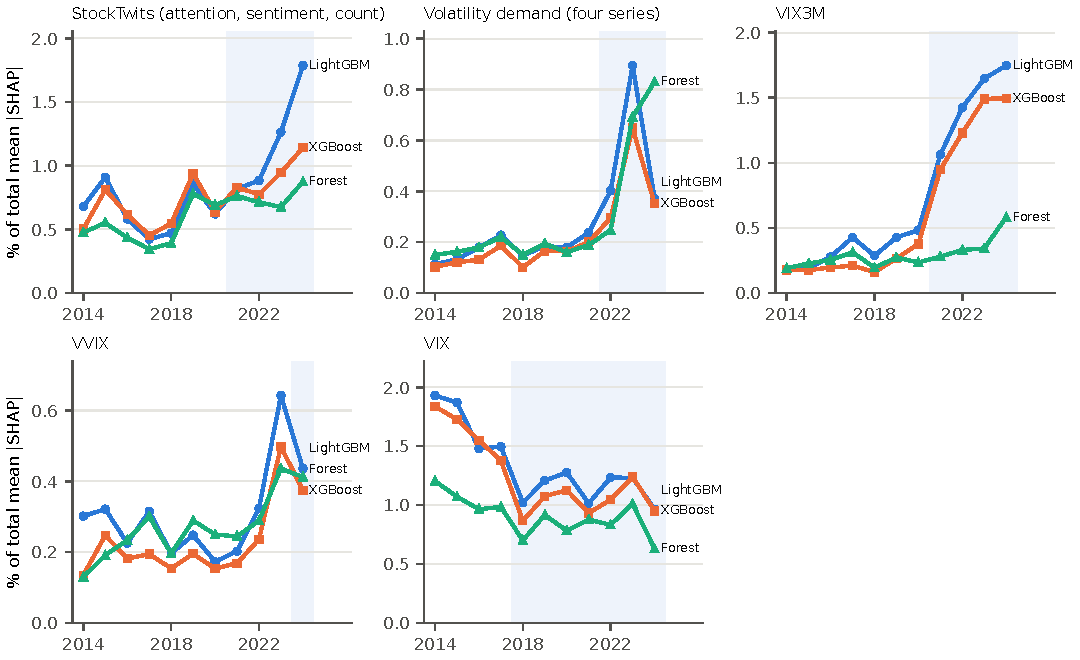
\includegraphics[width=\linewidth]{figures/fi_pooled/fi_live.pdf}
\caption{The late-starting series in the trees' attribution by calendar year: each group's share of the total mean absolute SHAP value, LightGBM, XGBoost and the random forest. Shaded: the years from the one in which the group's one-bar value average becomes nonzero under the late-start rule (Section~\ref{sec:rh_predictors}); before it, the group's attribution comes from its availability averages, which record when the series prints, not what it prints. 2024 covers January to April.}
\label{fig:rh_fi_live}
\end{figure}

\begin{itemize}
\item \textbf{Rankings} (Figure~\ref{fig:rh_fip_rank}, Table~\ref{tab:rh_fip_nonstd}). The ridge ranks the series
  differently from the trees. Its largest exogenous series is \rhfipRidgeTopOne{} (\rhfipRidgeTopOneEx\% of its
  exogenous total), where \rhfipTreeTopOne{} leads in every tree (\rhfipLgbmTopOneEx, \rhfipXgbTopOneEx{} and
  \rhfipRfTopOneEx\% of the exogenous total). Spearman rank correlation of the \rhfipNExog{} shares with the ridge's:
  \rhfipLgbmSpRidge, \rhfipXgbSpRidge, \rhfipRfSpRidge{} (the two top-\rhfipTopN{} lists share \rhfipLgbmTopRidge,
  \rhfipXgbTopRidge{} and \rhfipRfTopRidge{} series); among the trees: \rhfipSpLgbmXgb{} (LightGBM, XGBoost),
  \rhfipSpLgbmRf{} and \rhfipSpXgbRf{} (each against the forest). The remaining non-standard series carry little:
  VVIX \rhfipVvixMin--\rhfipVvixMax\% of the total, VIX3M \rhfipVixThreeMMin--\rhfipVixThreeMMax\%.
\item \textbf{Over time} (Figure~\ref{fig:rh_fip_time}). Every tree's non-standard share falls below its pooled value
  from \rhfipDipFirst{} to \rhfipDipLast{} and is lowest in \rhfipNsYearMinYr{} (\rhfipLgbmNsYearMin,
  \rhfipXgbNsYearMin{} and \rhfipRfNsYearMin\% of the total); the HAR components gain in the same years (LightGBM:
  \rhfipLgbmHarYearMax\% in \rhfipLgbmHarYearMaxYr, against \rhfipLgbmHarYearMin\% in \rhfipLgbmHarYearMinYr). The
  ridge's non-standard share of its exogenous total also dips, to its lowest in \rhfipRidgeNsExYearMinYr{}
  (\rhfipRidgeNsExYearMin\%, against \rhfipRidgeNsExYearMax\% in \rhfipRidgeNsExYearMaxYr; linear models dated by
  the origin). Panels (b) and (c) show the leading series year by year.
\end{itemize}
% The leading non-standard series: share, rank (trees, ridge), response shape, interaction fraction
% AUTO-GENERATED by writeup/make_rehaul_fi_pooled.py -- do not edit; re-run the script.
\providecommand{\ser}[2]{#2}\providecommand{\serx}[3]{#3}

\ifdefined\rhfipNOrigins\else% AUTO-GENERATED by writeup/make_rehaul_fi_pooled.py -- do not edit; re-run the script.
\providecommand{\ser}[2]{#2}\providecommand{\serx}[3]{#3}
% \rhfip... macros for writeup/rehaul/08_feature_importance.tex (results/tree_shap_w3000_2014start_fomcfix_2026-10-26, the
% FOMC-patched design, its linear reference inputs/fiw_gamma_fomcfix.npz; the window study's ...W... macros:
% results/fi_by_window_2014start_2026-10-22, pre-patch; the final pooled runs, W = 3,000 trading days).
\providecommand{\rhfipNOrigins}{}\renewcommand{\rhfipNOrigins}{126}  % monthly origins (re-estimations explained)
\providecommand{\rhfipNRows}{}\renewcommand{\rhfipNRows}{33{,}970}  % bars explained, every bar of the evaluation span
\providecommand{\rhfipOriginEvery}{}\renewcommand{\rhfipOriginEvery}{21}  % trading days between origins
\providecommand{\rhfipLastBlock}{}\renewcommand{\rhfipLastBlock}{18}  % trading days of the last origin's block
\providecommand{\rhfipFirstOrigin}{}\renewcommand{\rhfipFirstOrigin}{2~January~2014}  % first origin (10:00 bar)
\providecommand{\rhfipLastOrigin}{}\renewcommand{\rhfipLastOrigin}{5~April~2024}  % last origin
\providecommand{\rhfipLastDay}{}\renewcommand{\rhfipLastDay}{30~April~2024}  % day of the last bar explained
\providecommand{\rhfipWindowDays}{}\renewcommand{\rhfipWindowDays}{3{,}000}  % rolling window, trading days
\providecommand{\rhfipWindowBars}{}\renewcommand{\rhfipWindowBars}{39{,}000}  % rolling window, bars
\providecommand{\rhfipNCols}{}\renewcommand{\rhfipNCols}{564}  % predictors of the full set
\providecommand{\rhfipNGroups}{}\renewcommand{\rhfipNGroups}{48}  % predictor groups: 46 exogenous series + HAR components + calendar dummies
\providecommand{\rhfipNExog}{}\renewcommand{\rhfipNExog}{46}  % exogenous series
\providecommand{\rhfipNPerSeries}{}\renewcommand{\rhfipNPerSeries}{12}  % predictors per exogenous series: value and availability averages at six horizons
\providecommand{\rhfipNStd}{}\renewcommand{\rhfipNStd}{12}  % standard groups
\providecommand{\rhfipNNonStd}{}\renewcommand{\rhfipNNonStd}{36}  % non-standard series
\providecommand{\rhfipNStdExog}{}\renewcommand{\rhfipNStdExog}{10}  % standard exogenous series
\providecommand{\rhfipTuneLast}{}\renewcommand{\rhfipTuneLast}{31~December~2013}  % last day of the last tuning fold (fold 3)
\providecommand{\rhfipRidgePen}{}\renewcommand{\rhfipRidgePen}{\ensuremath{10^{3}}}
\providecommand{\rhfipLassoPen}{}\renewcommand{\rhfipLassoPen}{\ensuremath{10^{-4}}}
\providecommand{\rhfipEnetPen}{}\renewcommand{\rhfipEnetPen}{\ensuremath{10^{-3}}}
\providecommand{\rhfipHarPf}{}\renewcommand{\rhfipHarPf}{0.01}  % penalty factor, HAR block
\providecommand{\rhfipBootBlock}{}\renewcommand{\rhfipBootBlock}{12}  % bootstrap block, origins
\providecommand{\rhfipBootB}{}\renewcommand{\rhfipBootB}{2{,}000}
\providecommand{\rhfipCiLevel}{}\renewcommand{\rhfipCiLevel}{95}  % percentile intervals of both rules (RULE_shap.txt, RULE_fiw.txt)
\providecommand{\rhfipShapeMin}{}\renewcommand{\rhfipShapeMin}{0.5}  % M3 selection: share of at least this many percent
\providecommand{\rhfipTopN}{}\renewcommand{\rhfipTopN}{10}  % length of the top lists compared (m2_rank.csv top10_overlap)
\providecommand{\rhfipSlopeUnit}{}\renewcommand{\rhfipSlopeUnit}{1{,}000}  % trading days per unit of the window slope
\providecommand{\rhfipNMom}{}\renewcommand{\rhfipNMom}{seven}  % the futures' realized moments (standard)
\providecommand{\rhfipLgbmGateEq}{}\renewcommand{\rhfipLgbmGateEq}{126}  % origins bit-equal to the merged every-bar walk
\providecommand{\rhfipXgbGateEq}{}\renewcommand{\rhfipXgbGateEq}{126}  % origins bit-equal to the merged every-bar walk
\providecommand{\rhfipRfGateEq}{}\renewcommand{\rhfipRfGateEq}{126}  % origins bit-equal to the merged every-bar walk
\providecommand{\rhfipRfGateAtShap}{}\renewcommand{\rhfipRfGateAtShap}{126}  % forest origins the walk had written when the SHAP gate ran
\providecommand{\rhfipXgbAddMax}{}\renewcommand{\rhfipXgbAddMax}{\ensuremath{3.7\times 10^{-6}}}  % XGBoost additivity, float32
\providecommand{\rhfipXgbAddTol}{}\renewcommand{\rhfipXgbAddTol}{\ensuremath{10^{-5}}}
\providecommand{\rhfipAddMaxDouble}{}\renewcommand{\rhfipAddMaxDouble}{\ensuremath{5.1\times 10^{-14}}}
\providecommand{\rhfipLinGateMax}{}\renewcommand{\rhfipLinGateMax}{\ensuremath{4.4\times 10^{-16}}}  % linear replay vs walk forecasts, W = 3,000
\providecommand{\rhfipInterRows}{}\renewcommand{\rhfipInterRows}{1{,}008}  % M5 rows
\providecommand{\rhfipInterPerOrigin}{}\renewcommand{\rhfipInterPerOrigin}{8}  % M5 rows per origin
\providecommand{\rhfipFomcRows}{}\renewcommand{\rhfipFomcRows}{1{,}014}
\providecommand{\rhfipFomcDaysShap}{}\renewcommand{\rhfipFomcDaysShap}{78}  % FOMC statement days in the SHAP subset (M4; releases.parquet only)
\providecommand{\rhfipFomcDays}{}\renewcommand{\rhfipFomcDays}{81}  % scheduled FOMC statement days in the span (loader calendar)
\providecommand{\rhfipFomcDaysMissing}{}\renewcommand{\rhfipFomcDaysMissing}{3}  % statement days the SHAP subset leaves out (counted with the other days; the patched rerun's reducer keeps releases.parquet's days)
\providecommand{\rhfipNHolSessions}{}\renewcommand{\rhfipNHolSessions}{64}  % NYSE-holiday futures sessions among the explained bars (not scored in Table 1)
\providecommand{\rhfipNHolBars}{}\renewcommand{\rhfipNHolBars}{443}  % their regular-hours bars
\providecommand{\rhfipVixLo}{}\renewcommand{\rhfipVixLo}{13.96}
\providecommand{\rhfipVixHi}{}\renewcommand{\rhfipVixHi}{19.02}
\providecommand{\rhfipLgbmHar}{}\renewcommand{\rhfipLgbmHar}{51.7}
\providecommand{\rhfipLgbmHarLo}{}\renewcommand{\rhfipLgbmHarLo}{49.5}
\providecommand{\rhfipLgbmHarHi}{}\renewcommand{\rhfipLgbmHarHi}{53.7}
\providecommand{\rhfipLgbmMom}{}\renewcommand{\rhfipLgbmMom}{22.3}
\providecommand{\rhfipLgbmNs}{}\renewcommand{\rhfipLgbmNs}{21.8}
\providecommand{\rhfipLgbmNsLo}{}\renewcommand{\rhfipLgbmNsLo}{20.4}
\providecommand{\rhfipLgbmNsHi}{}\renewcommand{\rhfipLgbmNsHi}{23.4}
\providecommand{\rhfipLgbmNsEx}{}\renewcommand{\rhfipLgbmNsEx}{45.9}
\providecommand{\rhfipLgbmNsExLo}{}\renewcommand{\rhfipLgbmNsExLo}{44.2}
\providecommand{\rhfipLgbmNsExHi}{}\renewcommand{\rhfipLgbmNsExHi}{47.7}
\providecommand{\rhfipXgbHar}{}\renewcommand{\rhfipXgbHar}{52.0}
\providecommand{\rhfipXgbHarLo}{}\renewcommand{\rhfipXgbHarLo}{50.0}
\providecommand{\rhfipXgbHarHi}{}\renewcommand{\rhfipXgbHarHi}{53.8}
\providecommand{\rhfipXgbMom}{}\renewcommand{\rhfipXgbMom}{23.6}
\providecommand{\rhfipXgbNs}{}\renewcommand{\rhfipXgbNs}{20.6}
\providecommand{\rhfipXgbNsLo}{}\renewcommand{\rhfipXgbNsLo}{19.2}
\providecommand{\rhfipXgbNsHi}{}\renewcommand{\rhfipXgbNsHi}{22.2}
\providecommand{\rhfipXgbNsEx}{}\renewcommand{\rhfipXgbNsEx}{43.6}
\providecommand{\rhfipXgbNsExLo}{}\renewcommand{\rhfipXgbNsExLo}{41.8}
\providecommand{\rhfipXgbNsExHi}{}\renewcommand{\rhfipXgbNsExHi}{45.7}
\providecommand{\rhfipRfHar}{}\renewcommand{\rhfipRfHar}{57.6}
\providecommand{\rhfipRfHarLo}{}\renewcommand{\rhfipRfHarLo}{55.4}
\providecommand{\rhfipRfHarHi}{}\renewcommand{\rhfipRfHarHi}{59.6}
\providecommand{\rhfipRfMom}{}\renewcommand{\rhfipRfMom}{20.7}
\providecommand{\rhfipRfNs}{}\renewcommand{\rhfipRfNs}{18.6}
\providecommand{\rhfipRfNsLo}{}\renewcommand{\rhfipRfNsLo}{17.2}
\providecommand{\rhfipRfNsHi}{}\renewcommand{\rhfipRfNsHi}{20.3}
\providecommand{\rhfipRfNsEx}{}\renewcommand{\rhfipRfNsEx}{44.2}
\providecommand{\rhfipRfNsExLo}{}\renewcommand{\rhfipRfNsExLo}{42.1}
\providecommand{\rhfipRfNsExHi}{}\renewcommand{\rhfipRfNsExHi}{46.5}
\providecommand{\rhfipRidgeNsEx}{}\renewcommand{\rhfipRidgeNsEx}{68.8}
\providecommand{\rhfipRidgeNs}{}\renewcommand{\rhfipRidgeNs}{55.6}
\providecommand{\rhfipRidgeHar}{}\renewcommand{\rhfipRidgeHar}{17.5}
\providecommand{\rhfipLassoNsEx}{}\renewcommand{\rhfipLassoNsEx}{82.5}
\providecommand{\rhfipLassoNs}{}\renewcommand{\rhfipLassoNs}{76.5}
\providecommand{\rhfipLassoHar}{}\renewcommand{\rhfipLassoHar}{6.7}
\providecommand{\rhfipEnetNsEx}{}\renewcommand{\rhfipEnetNsEx}{60.0}
\providecommand{\rhfipEnetNs}{}\renewcommand{\rhfipEnetNs}{42.9}
\providecommand{\rhfipEnetHar}{}\renewcommand{\rhfipEnetHar}{26.4}
\providecommand{\rhfipHarMin}{}\renewcommand{\rhfipHarMin}{51.7}
\providecommand{\rhfipHarMax}{}\renewcommand{\rhfipHarMax}{57.6}
\providecommand{\rhfipMomMin}{}\renewcommand{\rhfipMomMin}{20.7}
\providecommand{\rhfipMomMax}{}\renewcommand{\rhfipMomMax}{23.6}
\providecommand{\rhfipNsExMin}{}\renewcommand{\rhfipNsExMin}{43.6}
\providecommand{\rhfipNsExMax}{}\renewcommand{\rhfipNsExMax}{45.9}
\providecommand{\rhfipSentMin}{}\renewcommand{\rhfipSentMin}{0.6}
\providecommand{\rhfipSentMax}{}\renewcommand{\rhfipSentMax}{0.8}
\providecommand{\rhfipVdMin}{}\renewcommand{\rhfipVdMin}{0.2}
\providecommand{\rhfipVdMax}{}\renewcommand{\rhfipVdMax}{0.3}
\providecommand{\rhfipFomcBucketMin}{}\renewcommand{\rhfipFomcBucketMin}{1.4}
\providecommand{\rhfipFomcBucketMax}{}\renewcommand{\rhfipFomcBucketMax}{2.3}
\providecommand{\rhfipVvixMin}{}\renewcommand{\rhfipVvixMin}{0.2}
\providecommand{\rhfipVvixMax}{}\renewcommand{\rhfipVvixMax}{0.3}
\providecommand{\rhfipVixThreeMMin}{}\renewcommand{\rhfipVixThreeMMin}{0.3}
\providecommand{\rhfipVixThreeMMax}{}\renewcommand{\rhfipVixThreeMMax}{0.7}
\providecommand{\rhfipFomcDayMin}{}\renewcommand{\rhfipFomcDayMin}{0.1}
\providecommand{\rhfipFomcDayMax}{}\renewcommand{\rhfipFomcDayMax}{0.1}
\providecommand{\rhfipNsOne}{}\renewcommand{\rhfipNsOne}{\ensuremath{\ser{sumabsret_vwstock}{\mathrm{RAV}^{\mathrm{VW}}}}}
\providecommand{\rhfipNsOneMin}{}\renewcommand{\rhfipNsOneMin}{2.4}
\providecommand{\rhfipNsOneMax}{}\renewcommand{\rhfipNsOneMax}{3.9}
\providecommand{\rhfipNsOneLgbm}{}\renewcommand{\rhfipNsOneLgbm}{3.5}
\providecommand{\rhfipNsOneXgb}{}\renewcommand{\rhfipNsOneXgb}{3.9}
\providecommand{\rhfipNsOneRf}{}\renewcommand{\rhfipNsOneRf}{2.4}
\providecommand{\rhfipNsTwo}{}\renewcommand{\rhfipNsTwo}{\ensuremath{\ser{sumabsret_ewstock}{\mathrm{RAV}^{\mathrm{EW}}}}}
\providecommand{\rhfipNsTwoMin}{}\renewcommand{\rhfipNsTwoMin}{1.9}
\providecommand{\rhfipNsTwoMax}{}\renewcommand{\rhfipNsTwoMax}{3.9}
\providecommand{\rhfipNsTwoLgbm}{}\renewcommand{\rhfipNsTwoLgbm}{3.9}
\providecommand{\rhfipNsTwoXgb}{}\renewcommand{\rhfipNsTwoXgb}{3.8}
\providecommand{\rhfipNsTwoRf}{}\renewcommand{\rhfipNsTwoRf}{1.9}
\providecommand{\rhfipNsThree}{}\renewcommand{\rhfipNsThree}{\ensuremath{\ser{fomc_until_inv}{\mathrm{FOMC}^{\mathrm{next}}}}}
\providecommand{\rhfipNsThreeMin}{}\renewcommand{\rhfipNsThreeMin}{1.1}
\providecommand{\rhfipNsThreeMax}{}\renewcommand{\rhfipNsThreeMax}{2.0}
\providecommand{\rhfipNsThreeLgbm}{}\renewcommand{\rhfipNsThreeLgbm}{2.0}
\providecommand{\rhfipNsThreeXgb}{}\renewcommand{\rhfipNsThreeXgb}{2.0}
\providecommand{\rhfipNsThreeRf}{}\renewcommand{\rhfipNsThreeRf}{1.1}
\providecommand{\rhfipNsFour}{}\renewcommand{\rhfipNsFour}{\ensuremath{\ser{ofi_vwstock}{\mathrm{OFI}^{\mathrm{VW}}}}}
\providecommand{\rhfipNsFourMin}{}\renewcommand{\rhfipNsFourMin}{1.4}
\providecommand{\rhfipNsFourMax}{}\renewcommand{\rhfipNsFourMax}{1.8}
\providecommand{\rhfipNsFourLgbm}{}\renewcommand{\rhfipNsFourLgbm}{1.8}
\providecommand{\rhfipNsFourXgb}{}\renewcommand{\rhfipNsFourXgb}{1.7}
\providecommand{\rhfipNsFourRf}{}\renewcommand{\rhfipNsFourRf}{1.4}
\providecommand{\rhfipNsFive}{}\renewcommand{\rhfipNsFive}{\ensuremath{\ser{effspread_vwstock}{\mathrm{EffSpread}^{\mathrm{VW}}}}}
\providecommand{\rhfipNsFiveMin}{}\renewcommand{\rhfipNsFiveMin}{1.2}
\providecommand{\rhfipNsFiveMax}{}\renewcommand{\rhfipNsFiveMax}{1.3}
\providecommand{\rhfipNsFiveLgbm}{}\renewcommand{\rhfipNsFiveLgbm}{1.2}
\providecommand{\rhfipNsFiveXgb}{}\renewcommand{\rhfipNsFiveXgb}{1.2}
\providecommand{\rhfipNsFiveRf}{}\renewcommand{\rhfipNsFiveRf}{1.3}
\providecommand{\rhfipTreeTopOne}{}\renewcommand{\rhfipTreeTopOne}{\ensuremath{\ser{sumabsret}{\mathrm{RAV}}}}
\providecommand{\rhfipTreeTopTwo}{}\renewcommand{\rhfipTreeTopTwo}{\ensuremath{\ser{sumret}{r}}}
\providecommand{\rhfipLgbmTopOneEx}{}\renewcommand{\rhfipLgbmTopOneEx}{20.3}
\providecommand{\rhfipXgbTopOneEx}{}\renewcommand{\rhfipXgbTopOneEx}{24.7}
\providecommand{\rhfipRfTopOneEx}{}\renewcommand{\rhfipRfTopOneEx}{29.2}
\providecommand{\rhfipRidgeTopOne}{}\renewcommand{\rhfipRidgeTopOne}{\ensuremath{\ser{fomc_until_inv}{\mathrm{FOMC}^{\mathrm{next}}}}}
\providecommand{\rhfipRidgeTopOneEx}{}\renewcommand{\rhfipRidgeTopOneEx}{9.0}
\providecommand{\rhfipLgbmNUsedAll}{}\renewcommand{\rhfipLgbmNUsedAll}{42}  % exogenous series split on at every origin
\providecommand{\rhfipLgbmUsedMin}{}\renewcommand{\rhfipLgbmUsedMin}{58}
\providecommand{\rhfipXgbNUsedAll}{}\renewcommand{\rhfipXgbNUsedAll}{43}  % exogenous series split on at every origin
\providecommand{\rhfipXgbUsedMin}{}\renewcommand{\rhfipXgbUsedMin}{72}
\providecommand{\rhfipRfNUsedAll}{}\renewcommand{\rhfipRfNUsedAll}{46}  % exogenous series split on at every origin
\providecommand{\rhfipRfUsedMin}{}\renewcommand{\rhfipRfUsedMin}{126}
\providecommand{\rhfipLgbmDRidge}{}\renewcommand{\rhfipLgbmDRidge}{\ensuremath{-}22.9}
\providecommand{\rhfipLgbmDRidgeLo}{}\renewcommand{\rhfipLgbmDRidgeLo}{\ensuremath{-}24.8}
\providecommand{\rhfipLgbmDRidgeHi}{}\renewcommand{\rhfipLgbmDRidgeHi}{\ensuremath{-}21.1}
\providecommand{\rhfipLgbmDLasso}{}\renewcommand{\rhfipLgbmDLasso}{\ensuremath{-}36.6}
\providecommand{\rhfipLgbmDLassoLo}{}\renewcommand{\rhfipLgbmDLassoLo}{\ensuremath{-}39.1}
\providecommand{\rhfipLgbmDLassoHi}{}\renewcommand{\rhfipLgbmDLassoHi}{\ensuremath{-}34.4}
\providecommand{\rhfipLgbmDEnet}{}\renewcommand{\rhfipLgbmDEnet}{\ensuremath{-}14.1}
\providecommand{\rhfipLgbmDEnetLo}{}\renewcommand{\rhfipLgbmDEnetLo}{\ensuremath{-}15.7}
\providecommand{\rhfipLgbmDEnetHi}{}\renewcommand{\rhfipLgbmDEnetHi}{\ensuremath{-}12.7}
\providecommand{\rhfipXgbDRidge}{}\renewcommand{\rhfipXgbDRidge}{\ensuremath{-}25.1}
\providecommand{\rhfipXgbDRidgeLo}{}\renewcommand{\rhfipXgbDRidgeLo}{\ensuremath{-}27.0}
\providecommand{\rhfipXgbDRidgeHi}{}\renewcommand{\rhfipXgbDRidgeHi}{\ensuremath{-}23.3}
\providecommand{\rhfipXgbDLasso}{}\renewcommand{\rhfipXgbDLasso}{\ensuremath{-}38.9}
\providecommand{\rhfipXgbDLassoLo}{}\renewcommand{\rhfipXgbDLassoLo}{\ensuremath{-}41.4}
\providecommand{\rhfipXgbDLassoHi}{}\renewcommand{\rhfipXgbDLassoHi}{\ensuremath{-}36.6}
\providecommand{\rhfipXgbDEnet}{}\renewcommand{\rhfipXgbDEnet}{\ensuremath{-}16.3}
\providecommand{\rhfipXgbDEnetLo}{}\renewcommand{\rhfipXgbDEnetLo}{\ensuremath{-}17.8}
\providecommand{\rhfipXgbDEnetHi}{}\renewcommand{\rhfipXgbDEnetHi}{\ensuremath{-}14.9}
\providecommand{\rhfipRfDRidge}{}\renewcommand{\rhfipRfDRidge}{\ensuremath{-}24.5}
\providecommand{\rhfipRfDRidgeLo}{}\renewcommand{\rhfipRfDRidgeLo}{\ensuremath{-}26.3}
\providecommand{\rhfipRfDRidgeHi}{}\renewcommand{\rhfipRfDRidgeHi}{\ensuremath{-}22.9}
\providecommand{\rhfipRfDLasso}{}\renewcommand{\rhfipRfDLasso}{\ensuremath{-}38.3}
\providecommand{\rhfipRfDLassoLo}{}\renewcommand{\rhfipRfDLassoLo}{\ensuremath{-}40.5}
\providecommand{\rhfipRfDLassoHi}{}\renewcommand{\rhfipRfDLassoHi}{\ensuremath{-}36.3}
\providecommand{\rhfipRfDEnet}{}\renewcommand{\rhfipRfDEnet}{\ensuremath{-}15.7}
\providecommand{\rhfipRfDEnetLo}{}\renewcommand{\rhfipRfDEnetLo}{\ensuremath{-}17.0}
\providecommand{\rhfipRfDEnetHi}{}\renewcommand{\rhfipRfDEnetHi}{\ensuremath{-}14.4}
\providecommand{\rhfipNDLess}{}\renewcommand{\rhfipNDLess}{27}  % tree-minus-linear D with the 95% interval below 0
\providecommand{\rhfipNDAll}{}\renewcommand{\rhfipNDAll}{27}  % D comparisons: 3 trees x 3 linear models x 3 denominators
\providecommand{\rhfipLgbmSpRidge}{}\renewcommand{\rhfipLgbmSpRidge}{0.57}
\providecommand{\rhfipLgbmTopRidge}{}\renewcommand{\rhfipLgbmTopRidge}{6}
\providecommand{\rhfipLgbmSpLasso}{}\renewcommand{\rhfipLgbmSpLasso}{0.49}
\providecommand{\rhfipLgbmTopLasso}{}\renewcommand{\rhfipLgbmTopLasso}{5}
\providecommand{\rhfipLgbmSpEnet}{}\renewcommand{\rhfipLgbmSpEnet}{0.66}
\providecommand{\rhfipLgbmTopEnet}{}\renewcommand{\rhfipLgbmTopEnet}{6}
\providecommand{\rhfipXgbSpRidge}{}\renewcommand{\rhfipXgbSpRidge}{0.55}
\providecommand{\rhfipXgbTopRidge}{}\renewcommand{\rhfipXgbTopRidge}{6}
\providecommand{\rhfipXgbSpLasso}{}\renewcommand{\rhfipXgbSpLasso}{0.47}
\providecommand{\rhfipXgbTopLasso}{}\renewcommand{\rhfipXgbTopLasso}{5}
\providecommand{\rhfipXgbSpEnet}{}\renewcommand{\rhfipXgbSpEnet}{0.63}
\providecommand{\rhfipXgbTopEnet}{}\renewcommand{\rhfipXgbTopEnet}{6}
\providecommand{\rhfipRfSpRidge}{}\renewcommand{\rhfipRfSpRidge}{0.53}
\providecommand{\rhfipRfTopRidge}{}\renewcommand{\rhfipRfTopRidge}{5}
\providecommand{\rhfipRfSpLasso}{}\renewcommand{\rhfipRfSpLasso}{0.43}
\providecommand{\rhfipRfTopLasso}{}\renewcommand{\rhfipRfTopLasso}{4}
\providecommand{\rhfipRfSpEnet}{}\renewcommand{\rhfipRfSpEnet}{0.60}
\providecommand{\rhfipRfTopEnet}{}\renewcommand{\rhfipRfTopEnet}{5}
\providecommand{\rhfipSpLgbmXgb}{}\renewcommand{\rhfipSpLgbmXgb}{0.99}
\providecommand{\rhfipSpLgbmRf}{}\renewcommand{\rhfipSpLgbmRf}{0.90}
\providecommand{\rhfipSpXgbRf}{}\renewcommand{\rhfipSpXgbRf}{0.89}
\providecommand{\rhfipRidgeRankFomcUntil}{}\renewcommand{\rhfipRidgeRankFomcUntil}{1}
\providecommand{\rhfipTreeRankFomcUntilMin}{}\renewcommand{\rhfipTreeRankFomcUntilMin}{6}
\providecommand{\rhfipTreeRankFomcUntilMax}{}\renewcommand{\rhfipTreeRankFomcUntilMax}{10}
\providecommand{\rhfipRidgeRankFomcDay}{}\renewcommand{\rhfipRidgeRankFomcDay}{9}
\providecommand{\rhfipTreeRankFomcDayMin}{}\renewcommand{\rhfipTreeRankFomcDayMin}{39}
\providecommand{\rhfipTreeRankFomcDayMax}{}\renewcommand{\rhfipTreeRankFomcDayMax}{43}
\providecommand{\rhfipFomcUntil}{}\renewcommand{\rhfipFomcUntil}{\ensuremath{\ser{fomc_until_inv}{\mathrm{FOMC}^{\mathrm{next}}}}}
\providecommand{\rhfipFomcDay}{}\renewcommand{\rhfipFomcDay}{\ensuremath{\ser{fomc_day}{\mathrm{FOMC}^{\mathrm{day}}}}}
\providecommand{\rhfipAbsVw}{}\renewcommand{\rhfipAbsVw}{\ensuremath{\ser{sumabsret_vwstock}{\mathrm{RAV}^{\mathrm{VW}}}}}
\providecommand{\rhfipOfi}{}\renewcommand{\rhfipOfi}{\ensuremath{\ser{ofi_vwstock}{\mathrm{OFI}^{\mathrm{VW}}}}}
\providecommand{\rhfipLgbmNeff}{}\renewcommand{\rhfipLgbmNeff}{11.0}
\providecommand{\rhfipLgbmNHalf}{}\renewcommand{\rhfipLgbmNHalf}{4}
\providecommand{\rhfipLgbmNEighty}{}\renewcommand{\rhfipLgbmNEighty}{13}
\providecommand{\rhfipXgbNeff}{}\renewcommand{\rhfipXgbNeff}{9.1}
\providecommand{\rhfipXgbNHalf}{}\renewcommand{\rhfipXgbNHalf}{4}
\providecommand{\rhfipXgbNEighty}{}\renewcommand{\rhfipXgbNEighty}{11}
\providecommand{\rhfipRfNeff}{}\renewcommand{\rhfipRfNeff}{8.9}
\providecommand{\rhfipRfNHalf}{}\renewcommand{\rhfipRfNHalf}{4}
\providecommand{\rhfipRfNEighty}{}\renewcommand{\rhfipRfNEighty}{16}
\providecommand{\rhfipRidgeNeff}{}\renewcommand{\rhfipRidgeNeff}{28.5}
\providecommand{\rhfipRidgeNHalf}{}\renewcommand{\rhfipRidgeNHalf}{11}
\providecommand{\rhfipRidgeNEighty}{}\renewcommand{\rhfipRidgeNEighty}{26}
\providecommand{\rhfipLassoNeff}{}\renewcommand{\rhfipLassoNeff}{5.1}
\providecommand{\rhfipLassoNHalf}{}\renewcommand{\rhfipLassoNHalf}{2}
\providecommand{\rhfipLassoNEighty}{}\renewcommand{\rhfipLassoNEighty}{11}
\providecommand{\rhfipEnetNeff}{}\renewcommand{\rhfipEnetNeff}{16.2}
\providecommand{\rhfipEnetNHalf}{}\renewcommand{\rhfipEnetNHalf}{6}
\providecommand{\rhfipEnetNEighty}{}\renewcommand{\rhfipEnetNEighty}{15}
\providecommand{\rhfipYearFirst}{}\renewcommand{\rhfipYearFirst}{2014}
\providecommand{\rhfipYearLast}{}\renewcommand{\rhfipYearLast}{2024}
\providecommand{\rhfipLgbmNsYearMin}{}\renewcommand{\rhfipLgbmNsYearMin}{18.1}
\providecommand{\rhfipLgbmNsYearMinYr}{}\renewcommand{\rhfipLgbmNsYearMinYr}{2021}
\providecommand{\rhfipLgbmNsYearMax}{}\renewcommand{\rhfipLgbmNsYearMax}{25.6}
\providecommand{\rhfipLgbmNsYearMaxYr}{}\renewcommand{\rhfipLgbmNsYearMaxYr}{2015}
\providecommand{\rhfipLgbmHarYearMax}{}\renewcommand{\rhfipLgbmHarYearMax}{57.4}
\providecommand{\rhfipLgbmHarYearMaxYr}{}\renewcommand{\rhfipLgbmHarYearMaxYr}{2021}
\providecommand{\rhfipLgbmHarYearMin}{}\renewcommand{\rhfipLgbmHarYearMin}{44.6}
\providecommand{\rhfipLgbmHarYearMinYr}{}\renewcommand{\rhfipLgbmHarYearMinYr}{2017}
\providecommand{\rhfipXgbNsYearMin}{}\renewcommand{\rhfipXgbNsYearMin}{17.2}
\providecommand{\rhfipXgbNsYearMinYr}{}\renewcommand{\rhfipXgbNsYearMinYr}{2021}
\providecommand{\rhfipXgbNsYearMax}{}\renewcommand{\rhfipXgbNsYearMax}{24.3}
\providecommand{\rhfipXgbNsYearMaxYr}{}\renewcommand{\rhfipXgbNsYearMaxYr}{2015}
\providecommand{\rhfipXgbHarYearMax}{}\renewcommand{\rhfipXgbHarYearMax}{57.0}
\providecommand{\rhfipXgbHarYearMaxYr}{}\renewcommand{\rhfipXgbHarYearMaxYr}{2021}
\providecommand{\rhfipXgbHarYearMin}{}\renewcommand{\rhfipXgbHarYearMin}{45.8}
\providecommand{\rhfipXgbHarYearMinYr}{}\renewcommand{\rhfipXgbHarYearMinYr}{2017}
\providecommand{\rhfipRfNsYearMin}{}\renewcommand{\rhfipRfNsYearMin}{15.2}
\providecommand{\rhfipRfNsYearMinYr}{}\renewcommand{\rhfipRfNsYearMinYr}{2021}
\providecommand{\rhfipRfNsYearMax}{}\renewcommand{\rhfipRfNsYearMax}{22.9}
\providecommand{\rhfipRfNsYearMaxYr}{}\renewcommand{\rhfipRfNsYearMaxYr}{2015}
\providecommand{\rhfipRfHarYearMax}{}\renewcommand{\rhfipRfHarYearMax}{62.3}
\providecommand{\rhfipRfHarYearMaxYr}{}\renewcommand{\rhfipRfHarYearMaxYr}{2019}
\providecommand{\rhfipRfHarYearMin}{}\renewcommand{\rhfipRfHarYearMin}{50.4}
\providecommand{\rhfipRfHarYearMinYr}{}\renewcommand{\rhfipRfHarYearMinYr}{2017}
\providecommand{\rhfipNsYearMinYr}{}\renewcommand{\rhfipNsYearMinYr}{2021}  % the year of every tree's lowest non-standard share
\providecommand{\rhfipDipFirst}{}\renewcommand{\rhfipDipFirst}{2018}  % first of the years in which every tree's non-standard share is below its pooled share
\providecommand{\rhfipDipLast}{}\renewcommand{\rhfipDipLast}{2022}
\providecommand{\rhfipRidgeNsExYearMin}{}\renewcommand{\rhfipRidgeNsExYearMin}{65.1}
\providecommand{\rhfipRidgeNsExYearMinYr}{}\renewcommand{\rhfipRidgeNsExYearMinYr}{2021}
\providecommand{\rhfipRidgeNsExYearMax}{}\renewcommand{\rhfipRidgeNsExYearMax}{72.4}
\providecommand{\rhfipRidgeNsExYearMaxYr}{}\renewcommand{\rhfipRidgeNsExYearMaxYr}{2017}
\providecommand{\rhfipLassoNsExYearMin}{}\renewcommand{\rhfipLassoNsExYearMin}{77.1}
\providecommand{\rhfipLassoNsExYearMinYr}{}\renewcommand{\rhfipLassoNsExYearMinYr}{2021}
\providecommand{\rhfipLassoNsExYearMax}{}\renewcommand{\rhfipLassoNsExYearMax}{87.1}
\providecommand{\rhfipLassoNsExYearMaxYr}{}\renewcommand{\rhfipLassoNsExYearMaxYr}{2017}
\providecommand{\rhfipEnetNsExYearMin}{}\renewcommand{\rhfipEnetNsExYearMin}{56.1}
\providecommand{\rhfipEnetNsExYearMinYr}{}\renewcommand{\rhfipEnetNsExYearMinYr}{2019}
\providecommand{\rhfipEnetNsExYearMax}{}\renewcommand{\rhfipEnetNsExYearMax}{65.2}
\providecommand{\rhfipEnetNsExYearMaxYr}{}\renewcommand{\rhfipEnetNsExYearMaxYr}{2014}
\providecommand{\rhfipLgbmNsExYearMin}{}\renewcommand{\rhfipLgbmNsExYearMin}{42.3}
\providecommand{\rhfipLgbmNsExYearMax}{}\renewcommand{\rhfipLgbmNsExYearMax}{50.1}
\providecommand{\rhfipXgbNsExYearMin}{}\renewcommand{\rhfipXgbNsExYearMin}{39.4}
\providecommand{\rhfipXgbNsExYearMax}{}\renewcommand{\rhfipXgbNsExYearMax}{48.9}
\providecommand{\rhfipRfNsExYearMin}{}\renewcommand{\rhfipRfNsExYearMin}{39.5}
\providecommand{\rhfipRfNsExYearMax}{}\renewcommand{\rhfipRfNsExYearMax}{50.9}
\providecommand{\rhfipLgbmNShape}{}\renewcommand{\rhfipLgbmNShape}{11}  % non-standard series at >= 0.5% (M3)
\providecommand{\rhfipLgbmNMono}{}\renewcommand{\rhfipLgbmNMono}{7}
\providecommand{\rhfipLgbmNIrr}{}\renewcommand{\rhfipLgbmNIrr}{3}
\providecommand{\rhfipLgbmNStep}{}\renewcommand{\rhfipLgbmNStep}{1}
\providecommand{\rhfipLgbmNFlat}{}\renewcommand{\rhfipLgbmNFlat}{0}
\providecommand{\rhfipLgbmNThresh}{}\renewcommand{\rhfipLgbmNThresh}{0}
\providecommand{\rhfipLgbmNU}{}\renewcommand{\rhfipLgbmNU}{0}
\providecommand{\rhfipLgbmNAsym}{}\renewcommand{\rhfipLgbmNAsym}{9}
\providecommand{\rhfipXgbNShape}{}\renewcommand{\rhfipXgbNShape}{10}  % non-standard series at >= 0.5% (M3)
\providecommand{\rhfipXgbNMono}{}\renewcommand{\rhfipXgbNMono}{5}
\providecommand{\rhfipXgbNIrr}{}\renewcommand{\rhfipXgbNIrr}{3}
\providecommand{\rhfipXgbNStep}{}\renewcommand{\rhfipXgbNStep}{0}
\providecommand{\rhfipXgbNFlat}{}\renewcommand{\rhfipXgbNFlat}{1}
\providecommand{\rhfipXgbNThresh}{}\renewcommand{\rhfipXgbNThresh}{1}
\providecommand{\rhfipXgbNU}{}\renewcommand{\rhfipXgbNU}{0}
\providecommand{\rhfipXgbNAsym}{}\renewcommand{\rhfipXgbNAsym}{8}
\providecommand{\rhfipRfNShape}{}\renewcommand{\rhfipRfNShape}{13}  % non-standard series at >= 0.5% (M3)
\providecommand{\rhfipRfNMono}{}\renewcommand{\rhfipRfNMono}{10}
\providecommand{\rhfipRfNIrr}{}\renewcommand{\rhfipRfNIrr}{3}
\providecommand{\rhfipRfNStep}{}\renewcommand{\rhfipRfNStep}{0}
\providecommand{\rhfipRfNFlat}{}\renewcommand{\rhfipRfNFlat}{0}
\providecommand{\rhfipRfNThresh}{}\renewcommand{\rhfipRfNThresh}{0}
\providecommand{\rhfipRfNU}{}\renewcommand{\rhfipRfNU}{0}
\providecommand{\rhfipRfNAsym}{}\renewcommand{\rhfipRfNAsym}{13}
\providecommand{\rhfipNUThreshAll}{}\renewcommand{\rhfipNUThreshAll}{1}  % U-shaped, inverted-U or threshold profiles in any tree
\providecommand{\rhfipAbsVwLgbmLo}{}\renewcommand{\rhfipAbsVwLgbmLo}{\ensuremath{-}1.4}
\providecommand{\rhfipAbsVwLgbmHi}{}\renewcommand{\rhfipAbsVwLgbmHi}{3.9}
\providecommand{\rhfipAbsVwXgbLo}{}\renewcommand{\rhfipAbsVwXgbLo}{\ensuremath{-}1.5}
\providecommand{\rhfipAbsVwXgbHi}{}\renewcommand{\rhfipAbsVwXgbHi}{4.3}
\providecommand{\rhfipAbsVwRfLo}{}\renewcommand{\rhfipAbsVwRfLo}{\ensuremath{-}0.9}
\providecommand{\rhfipAbsVwRfHi}{}\renewcommand{\rhfipAbsVwRfHi}{2.3}
\providecommand{\rhfipOfiLgbmLo}{}\renewcommand{\rhfipOfiLgbmLo}{0.8}
\providecommand{\rhfipOfiLgbmHi}{}\renewcommand{\rhfipOfiLgbmHi}{\ensuremath{-}1.1}
\providecommand{\rhfipOfiXgbLo}{}\renewcommand{\rhfipOfiXgbLo}{0.8}
\providecommand{\rhfipOfiXgbHi}{}\renewcommand{\rhfipOfiXgbHi}{\ensuremath{-}0.9}
\providecommand{\rhfipOfiRfLo}{}\renewcommand{\rhfipOfiRfLo}{0.8}
\providecommand{\rhfipOfiRfHi}{}\renewcommand{\rhfipOfiRfHi}{\ensuremath{-}0.7}
\providecommand{\rhfipUntilLgbmLo}{}\renewcommand{\rhfipUntilLgbmLo}{\ensuremath{-}0.3}
\providecommand{\rhfipUntilLgbmHi}{}\renewcommand{\rhfipUntilLgbmHi}{2.9}
\providecommand{\rhfipUntilXgbLo}{}\renewcommand{\rhfipUntilXgbLo}{0.2}
\providecommand{\rhfipUntilXgbHi}{}\renewcommand{\rhfipUntilXgbHi}{2.4}
\providecommand{\rhfipUntilRfLo}{}\renewcommand{\rhfipUntilRfLo}{\ensuremath{-}0.0}
\providecommand{\rhfipUntilRfHi}{}\renewcommand{\rhfipUntilRfHi}{1.5}
\providecommand{\rhfipUntilHorizon}{}\renewcommand{\rhfipUntilHorizon}{25}  % horizon of fomc_until_inv's dominant column
\providecommand{\rhfipUntilHorizonXgb}{}\renewcommand{\rhfipUntilHorizonXgb}{1}  % the same in XGBoost (differs from the other trees')
\providecommand{\rhfipBarFirst}{}\renewcommand{\rhfipBarFirst}{10:00}
\providecommand{\rhfipBarLast}{}\renewcommand{\rhfipBarLast}{16:00}
\providecommand{\rhfipBarPeakA}{}\renewcommand{\rhfipBarPeakA}{14:30}
\providecommand{\rhfipBarPeakB}{}\renewcommand{\rhfipBarPeakB}{15:00}
\providecommand{\rhfipNBars}{}\renewcommand{\rhfipNBars}{13}
\providecommand{\rhfipLgbmNsFomc}{}\renewcommand{\rhfipLgbmNsFomc}{42.6}
\providecommand{\rhfipLgbmNsOther}{}\renewcommand{\rhfipLgbmNsOther}{20.9}
\providecommand{\rhfipLgbmUntilFomc}{}\renewcommand{\rhfipLgbmUntilFomc}{25.4}
\providecommand{\rhfipLgbmUntilOther}{}\renewcommand{\rhfipLgbmUntilOther}{1.06}
\providecommand{\rhfipLgbmFomcBucketFomc}{}\renewcommand{\rhfipLgbmFomcBucketFomc}{27.3}
\providecommand{\rhfipLgbmFomcBucketOther}{}\renewcommand{\rhfipLgbmFomcBucketOther}{1.3}
\providecommand{\rhfipLgbmHarFomc}{}\renewcommand{\rhfipLgbmHarFomc}{39.2}
\providecommand{\rhfipLgbmHarOther}{}\renewcommand{\rhfipLgbmHarOther}{52.2}
\providecommand{\rhfipLgbmNsFirstBar}{}\renewcommand{\rhfipLgbmNsFirstBar}{23.9}
\providecommand{\rhfipLgbmNsLastBar}{}\renewcommand{\rhfipLgbmNsLastBar}{20.5}
\providecommand{\rhfipLgbmNsAftMin}{}\renewcommand{\rhfipLgbmNsAftMin}{24.3}
\providecommand{\rhfipLgbmNsAftMax}{}\renewcommand{\rhfipLgbmNsAftMax}{25.2}
\providecommand{\rhfipLgbmNsMidMin}{}\renewcommand{\rhfipLgbmNsMidMin}{20.1}
\providecommand{\rhfipLgbmNsMidMax}{}\renewcommand{\rhfipLgbmNsMidMax}{21.9}
\providecommand{\rhfipLgbmFomcBucketAft}{}\renewcommand{\rhfipLgbmFomcBucketAft}{5.5}
\providecommand{\rhfipLgbmFomcBucketOtherBars}{}\renewcommand{\rhfipLgbmFomcBucketOtherBars}{1.4}  % median FOMC-announcement share over the other 11 bars
\providecommand{\rhfipLgbmFomcDiff}{}\renewcommand{\rhfipLgbmFomcDiff}{\ensuremath{+}21.7}
\providecommand{\rhfipLgbmFomcDiffLo}{}\renewcommand{\rhfipLgbmFomcDiffLo}{\ensuremath{+}19.3}
\providecommand{\rhfipLgbmFomcDiffHi}{}\renewcommand{\rhfipLgbmFomcDiffHi}{\ensuremath{+}24.1}
\providecommand{\rhfipLgbmLateDiff}{}\renewcommand{\rhfipLgbmLateDiff}{\ensuremath{-}3.4}
\providecommand{\rhfipLgbmLateDiffLo}{}\renewcommand{\rhfipLgbmLateDiffLo}{\ensuremath{-}4.3}
\providecommand{\rhfipLgbmLateDiffHi}{}\renewcommand{\rhfipLgbmLateDiffHi}{\ensuremath{-}2.5}
\providecommand{\rhfipLgbmVixDiff}{}\renewcommand{\rhfipLgbmVixDiff}{\ensuremath{-}3.2}
\providecommand{\rhfipLgbmVixDiffLo}{}\renewcommand{\rhfipLgbmVixDiffLo}{\ensuremath{-}5.3}
\providecommand{\rhfipLgbmVixDiffHi}{}\renewcommand{\rhfipLgbmVixDiffHi}{\ensuremath{-}1.1}
\providecommand{\rhfipLgbmVixHar}{}\renewcommand{\rhfipLgbmVixHar}{\ensuremath{+}5.1}
\providecommand{\rhfipLgbmVixHarLo}{}\renewcommand{\rhfipLgbmVixHarLo}{\ensuremath{+}1.8}
\providecommand{\rhfipLgbmVixHarHi}{}\renewcommand{\rhfipLgbmVixHarHi}{\ensuremath{+}8.4}
\providecommand{\rhfipLgbmVixDiffEx}{}\renewcommand{\rhfipLgbmVixDiffEx}{\ensuremath{-}2.3}
\providecommand{\rhfipLgbmVixDiffExLo}{}\renewcommand{\rhfipLgbmVixDiffExLo}{\ensuremath{-}4.5}
\providecommand{\rhfipLgbmVixDiffExHi}{}\renewcommand{\rhfipLgbmVixDiffExHi}{\ensuremath{-}0.2}
\providecommand{\rhfipXgbNsFomc}{}\renewcommand{\rhfipXgbNsFomc}{41.1}
\providecommand{\rhfipXgbNsOther}{}\renewcommand{\rhfipXgbNsOther}{19.7}
\providecommand{\rhfipXgbUntilFomc}{}\renewcommand{\rhfipXgbUntilFomc}{23.9}
\providecommand{\rhfipXgbUntilOther}{}\renewcommand{\rhfipXgbUntilOther}{1.10}
\providecommand{\rhfipXgbFomcBucketFomc}{}\renewcommand{\rhfipXgbFomcBucketFomc}{25.6}
\providecommand{\rhfipXgbFomcBucketOther}{}\renewcommand{\rhfipXgbFomcBucketOther}{1.3}
\providecommand{\rhfipXgbHarFomc}{}\renewcommand{\rhfipXgbHarFomc}{39.1}
\providecommand{\rhfipXgbHarOther}{}\renewcommand{\rhfipXgbHarOther}{52.5}
\providecommand{\rhfipXgbNsFirstBar}{}\renewcommand{\rhfipXgbNsFirstBar}{22.5}
\providecommand{\rhfipXgbNsLastBar}{}\renewcommand{\rhfipXgbNsLastBar}{19.5}
\providecommand{\rhfipXgbNsAftMin}{}\renewcommand{\rhfipXgbNsAftMin}{23.5}
\providecommand{\rhfipXgbNsAftMax}{}\renewcommand{\rhfipXgbNsAftMax}{23.7}
\providecommand{\rhfipXgbNsMidMin}{}\renewcommand{\rhfipXgbNsMidMin}{19.1}
\providecommand{\rhfipXgbNsMidMax}{}\renewcommand{\rhfipXgbNsMidMax}{20.4}
\providecommand{\rhfipXgbFomcBucketAft}{}\renewcommand{\rhfipXgbFomcBucketAft}{5.8}
\providecommand{\rhfipXgbFomcBucketOtherBars}{}\renewcommand{\rhfipXgbFomcBucketOtherBars}{1.3}  % median FOMC-announcement share over the other 11 bars
\providecommand{\rhfipXgbFomcDiff}{}\renewcommand{\rhfipXgbFomcDiff}{\ensuremath{+}21.4}
\providecommand{\rhfipXgbFomcDiffLo}{}\renewcommand{\rhfipXgbFomcDiffLo}{\ensuremath{+}19.3}
\providecommand{\rhfipXgbFomcDiffHi}{}\renewcommand{\rhfipXgbFomcDiffHi}{\ensuremath{+}23.5}
\providecommand{\rhfipXgbLateDiff}{}\renewcommand{\rhfipXgbLateDiff}{\ensuremath{-}3.1}
\providecommand{\rhfipXgbLateDiffLo}{}\renewcommand{\rhfipXgbLateDiffLo}{\ensuremath{-}4.0}
\providecommand{\rhfipXgbLateDiffHi}{}\renewcommand{\rhfipXgbLateDiffHi}{\ensuremath{-}2.3}
\providecommand{\rhfipXgbVixDiff}{}\renewcommand{\rhfipXgbVixDiff}{\ensuremath{-}3.0}
\providecommand{\rhfipXgbVixDiffLo}{}\renewcommand{\rhfipXgbVixDiffLo}{\ensuremath{-}5.1}
\providecommand{\rhfipXgbVixDiffHi}{}\renewcommand{\rhfipXgbVixDiffHi}{\ensuremath{-}0.9}
\providecommand{\rhfipXgbVixHar}{}\renewcommand{\rhfipXgbVixHar}{\ensuremath{+}3.9}
\providecommand{\rhfipXgbVixHarLo}{}\renewcommand{\rhfipXgbVixHarLo}{\ensuremath{+}0.4}
\providecommand{\rhfipXgbVixHarHi}{}\renewcommand{\rhfipXgbVixHarHi}{\ensuremath{+}7.2}
\providecommand{\rhfipXgbVixDiffEx}{}\renewcommand{\rhfipXgbVixDiffEx}{\ensuremath{-}3.2}
\providecommand{\rhfipXgbVixDiffExLo}{}\renewcommand{\rhfipXgbVixDiffExLo}{\ensuremath{-}5.7}
\providecommand{\rhfipXgbVixDiffExHi}{}\renewcommand{\rhfipXgbVixDiffExHi}{\ensuremath{-}0.8}
\providecommand{\rhfipRfNsFomc}{}\renewcommand{\rhfipRfNsFomc}{28.9}
\providecommand{\rhfipRfNsOther}{}\renewcommand{\rhfipRfNsOther}{18.3}
\providecommand{\rhfipRfUntilFomc}{}\renewcommand{\rhfipRfUntilFomc}{12.4}
\providecommand{\rhfipRfFomcBucketFomc}{}\renewcommand{\rhfipRfFomcBucketFomc}{13.0}
\providecommand{\rhfipRfFomcBucketOther}{}\renewcommand{\rhfipRfFomcBucketOther}{1.0}
\providecommand{\rhfipRfHarFomc}{}\renewcommand{\rhfipRfHarFomc}{50.8}
\providecommand{\rhfipRfHarOther}{}\renewcommand{\rhfipRfHarOther}{57.9}
\providecommand{\rhfipRfNsFirstBar}{}\renewcommand{\rhfipRfNsFirstBar}{20.1}
\providecommand{\rhfipRfNsLastBar}{}\renewcommand{\rhfipRfNsLastBar}{17.8}
\providecommand{\rhfipRfNsAftMin}{}\renewcommand{\rhfipRfNsAftMin}{19.5}
\providecommand{\rhfipRfNsAftMax}{}\renewcommand{\rhfipRfNsAftMax}{19.9}
\providecommand{\rhfipRfNsMidMin}{}\renewcommand{\rhfipRfNsMidMin}{17.8}
\providecommand{\rhfipRfNsMidMax}{}\renewcommand{\rhfipRfNsMidMax}{18.6}
\providecommand{\rhfipRfFomcBucketAft}{}\renewcommand{\rhfipRfFomcBucketAft}{3.1}
\providecommand{\rhfipRfFomcBucketOtherBars}{}\renewcommand{\rhfipRfFomcBucketOtherBars}{1.0}  % median FOMC-announcement share over the other 11 bars
\providecommand{\rhfipRfFomcDiff}{}\renewcommand{\rhfipRfFomcDiff}{\ensuremath{+}10.6}
\providecommand{\rhfipRfFomcDiffLo}{}\renewcommand{\rhfipRfFomcDiffLo}{\ensuremath{+}8.3}
\providecommand{\rhfipRfFomcDiffHi}{}\renewcommand{\rhfipRfFomcDiffHi}{\ensuremath{+}13.1}
\providecommand{\rhfipRfLateDiff}{}\renewcommand{\rhfipRfLateDiff}{\ensuremath{-}2.3}
\providecommand{\rhfipRfLateDiffLo}{}\renewcommand{\rhfipRfLateDiffLo}{\ensuremath{-}3.1}
\providecommand{\rhfipRfLateDiffHi}{}\renewcommand{\rhfipRfLateDiffHi}{\ensuremath{-}1.6}
\providecommand{\rhfipRfVixDiff}{}\renewcommand{\rhfipRfVixDiff}{\ensuremath{-}3.3}
\providecommand{\rhfipRfVixDiffLo}{}\renewcommand{\rhfipRfVixDiffLo}{\ensuremath{-}5.1}
\providecommand{\rhfipRfVixDiffHi}{}\renewcommand{\rhfipRfVixDiffHi}{\ensuremath{-}1.4}
\providecommand{\rhfipRfVixHar}{}\renewcommand{\rhfipRfVixHar}{\ensuremath{+}4.2}
\providecommand{\rhfipRfVixHarLo}{}\renewcommand{\rhfipRfVixHarLo}{\ensuremath{+}1.0}
\providecommand{\rhfipRfVixHarHi}{}\renewcommand{\rhfipRfVixHarHi}{\ensuremath{+}7.3}
\providecommand{\rhfipRfVixDiffEx}{}\renewcommand{\rhfipRfVixDiffEx}{\ensuremath{-}3.7}
\providecommand{\rhfipRfVixDiffExLo}{}\renewcommand{\rhfipRfVixDiffExLo}{\ensuremath{-}6.3}
\providecommand{\rhfipRfVixDiffExHi}{}\renewcommand{\rhfipRfVixDiffExHi}{\ensuremath{-}1.2}
\providecommand{\rhfipLgbmInterVar}{}\renewcommand{\rhfipLgbmInterVar}{33.1}
\providecommand{\rhfipLgbmInterCol}{}\renewcommand{\rhfipLgbmInterCol}{45.3}
\providecommand{\rhfipLgbmInterNs}{}\renewcommand{\rhfipLgbmInterNs}{49.6}
\providecommand{\rhfipLgbmInterStd}{}\renewcommand{\rhfipLgbmInterStd}{26.8}
\providecommand{\rhfipLgbmInterStdEx}{}\renewcommand{\rhfipLgbmInterStdEx}{40.2}  % descriptive: standard exogenous series only (no HAR, no calendar)
\providecommand{\rhfipLgbmInterHar}{}\renewcommand{\rhfipLgbmInterHar}{17.1}
\providecommand{\rhfipLgbmInterWeakMin}{}\renewcommand{\rhfipLgbmInterWeakMin}{54}
\providecommand{\rhfipLgbmInterWeakMax}{}\renewcommand{\rhfipLgbmInterWeakMax}{66}
\providecommand{\rhfipLgbmPairOne}{}\renewcommand{\rhfipLgbmPairOne}{1.25}
\providecommand{\rhfipLgbmPairTwo}{}\renewcommand{\rhfipLgbmPairTwo}{0.86}
\providecommand{\rhfipLgbmCellHarHar}{}\renewcommand{\rhfipLgbmCellHarHar}{48.0}
\providecommand{\rhfipXgbInterVar}{}\renewcommand{\rhfipXgbInterVar}{30.9}
\providecommand{\rhfipXgbInterCol}{}\renewcommand{\rhfipXgbInterCol}{42.5}
\providecommand{\rhfipXgbInterNs}{}\renewcommand{\rhfipXgbInterNs}{45.7}
\providecommand{\rhfipXgbInterStd}{}\renewcommand{\rhfipXgbInterStd}{26.0}
\providecommand{\rhfipXgbInterStdEx}{}\renewcommand{\rhfipXgbInterStdEx}{37.8}  % descriptive: standard exogenous series only (no HAR, no calendar)
\providecommand{\rhfipXgbInterHar}{}\renewcommand{\rhfipXgbInterHar}{17.6}
\providecommand{\rhfipXgbInterWeakMin}{}\renewcommand{\rhfipXgbInterWeakMin}{54}
\providecommand{\rhfipXgbInterWeakMax}{}\renewcommand{\rhfipXgbInterWeakMax}{63}
\providecommand{\rhfipXgbPairOne}{}\renewcommand{\rhfipXgbPairOne}{1.23}
\providecommand{\rhfipXgbPairTwo}{}\renewcommand{\rhfipXgbPairTwo}{0.83}
\providecommand{\rhfipXgbCellHarHar}{}\renewcommand{\rhfipXgbCellHarHar}{47.4}
\providecommand{\rhfipPairOneA}{}\renewcommand{\rhfipPairOneA}{HAR components}
\providecommand{\rhfipPairOneB}{}\renewcommand{\rhfipPairOneB}{\ensuremath{\ser{sumabsret_vwstock}{\mathrm{RAV}^{\mathrm{VW}}}}}
\providecommand{\rhfipPairTwoA}{}\renewcommand{\rhfipPairTwoA}{HAR components}
\providecommand{\rhfipPairTwoB}{}\renewcommand{\rhfipPairTwoB}{\ensuremath{\ser{sumabsret_ewstock}{\mathrm{RAV}^{\mathrm{EW}}}}}
\providecommand{\rhfipLgbmPairsHar}{}\renewcommand{\rhfipLgbmPairsHar}{7}
\providecommand{\rhfipXgbPairsHar}{}\renewcommand{\rhfipXgbPairsHar}{7}
\providecommand{\rhfipWMin}{}\renewcommand{\rhfipWMin}{1{,}000}
\providecommand{\rhfipWMax}{}\renewcommand{\rhfipWMax}{3{,}500}
\providecommand{\rhfipNWindows}{}\renewcommand{\rhfipNWindows}{6}
\providecommand{\rhfipSOneMeasures}{}\renewcommand{\rhfipSOneMeasures}{105}  % measure x common-penalty fits of the window study (P1 and P2)
\providecommand{\rhfipSOneRises}{}\renewcommand{\rhfipSOneRises}{0}  % ... of which rise with W
\providecommand{\rhfipSOneFalls}{}\renewcommand{\rhfipSOneFalls}{102}
\providecommand{\rhfipSOneFlat}{}\renewcommand{\rhfipSOneFlat}{3}
\providecommand{\rhfipSOneNotSupported}{}\renewcommand{\rhfipSOneNotSupported}{14}  % common-penalty verdicts NOT SUPPORTED
\providecommand{\rhfipSOneVerdicts}{}\renewcommand{\rhfipSOneVerdicts}{14}
\providecommand{\rhfipRidgeNeffWMin}{}\renewcommand{\rhfipRidgeNeffWMin}{29.2}
\providecommand{\rhfipRidgeNeffWMain}{}\renewcommand{\rhfipRidgeNeffWMain}{29.2}
\providecommand{\rhfipRidgeNeffWMax}{}\renewcommand{\rhfipRidgeNeffWMax}{28.2}
\providecommand{\rhfipRidgeNeffSlope}{}\renewcommand{\rhfipRidgeNeffSlope}{\ensuremath{-}0.10}
\providecommand{\rhfipRidgeNeffSlopeLo}{}\renewcommand{\rhfipRidgeNeffSlopeLo}{\ensuremath{-}0.25}
\providecommand{\rhfipRidgeNeffSlopeHi}{}\renewcommand{\rhfipRidgeNeffSlopeHi}{0.12}
\providecommand{\rhfipRidgeSOneLoNeffWMin}{}\renewcommand{\rhfipRidgeSOneLoNeffWMin}{33.9}
\providecommand{\rhfipRidgeSOneLoNeffWMax}{}\renewcommand{\rhfipRidgeSOneLoNeffWMax}{28.2}
\providecommand{\rhfipRidgeSOneHiNeffWMin}{}\renewcommand{\rhfipRidgeSOneHiNeffWMin}{29.2}
\providecommand{\rhfipRidgeSOneHiNeffWMax}{}\renewcommand{\rhfipRidgeSOneHiNeffWMax}{23.5}
\providecommand{\rhfipLassoSOneVWMin}{}\renewcommand{\rhfipLassoSOneVWMin}{38.7}
\providecommand{\rhfipLassoSOneVWMax}{}\renewcommand{\rhfipLassoSOneVWMax}{31.9}
\providecommand{\rhfipLassoSOneCWMin}{}\renewcommand{\rhfipLassoSOneCWMin}{213.3}
\providecommand{\rhfipLassoSOneCWMax}{}\renewcommand{\rhfipLassoSOneCWMax}{177.5}
\providecommand{\rhfipLassoWalkVWMin}{}\renewcommand{\rhfipLassoWalkVWMin}{38.8}
\providecommand{\rhfipLassoWalkVWMax}{}\renewcommand{\rhfipLassoWalkVWMax}{41.9}
\providecommand{\rhfipLassoSOneLo}{}\renewcommand{\rhfipLassoSOneLo}{\ensuremath{10^{-3}}}
\providecommand{\rhfipRidgeSOneLo}{}\renewcommand{\rhfipRidgeSOneLo}{\ensuremath{10^{3}}}
\providecommand{\rhfipRidgeSOneHi}{}\renewcommand{\rhfipRidgeSOneHi}{\ensuremath{10^{4}}}
\providecommand{\rhfipEnetPenWMin}{}\renewcommand{\rhfipEnetPenWMin}{\ensuremath{10^{-2}}}
\providecommand{\rhfipEnetPenWNext}{}\renewcommand{\rhfipEnetPenWNext}{\ensuremath{10^{-3}}}
\providecommand{\rhfipWNext}{}\renewcommand{\rhfipWNext}{1{,}500}
\providecommand{\rhfipRidgePOneWalk}{}\renewcommand{\rhfipRidgePOneWalk}{not supported}
\providecommand{\rhfipRidgePTwoWalk}{}\renewcommand{\rhfipRidgePTwoWalk}{not supported}
\providecommand{\rhfipLassoPOneWalk}{}\renewcommand{\rhfipLassoPOneWalk}{partly}
\providecommand{\rhfipLassoPTwoWalk}{}\renewcommand{\rhfipLassoPTwoWalk}{not supported}
\providecommand{\rhfipEnetPOneWalk}{}\renewcommand{\rhfipEnetPOneWalk}{supported}
\providecommand{\rhfipEnetPTwoWalk}{}\renewcommand{\rhfipEnetPTwoWalk}{supported}
\fi
\begin{table}[tbp]
\centering
\footnotesize
\setlength{\tabcolsep}{3.5pt}
\begin{threeparttable}
\caption{The leading non-standard series in the tree ensembles}
\label{tab:rh_fip_nonstd}
\begin{tabular}{@{}l rrr rr ccc rr@{}}
\toprule
 & \multicolumn{3}{c}{Share (\%)} & \multicolumn{2}{c}{Rank} & \multicolumn{3}{c}{Response shape} & \multicolumn{2}{c}{Interaction (\%)} \\
\cmidrule(lr){2-4}\cmidrule(lr){5-6}\cmidrule(lr){7-9}\cmidrule(l){10-11}
Series & LGBM & XGB & RF & Trees & Ridge & LGBM & XGB & RF & LGBM & XGB \\
\midrule
\multicolumn{11}{@{}l}{\textit{Panel A: Non-standard series with a share of at least \rhfipShapeMin\% in some tree ensemble}} \\
\ensuremath{\ser{sumabsret_vwstock}{\mathrm{RAV}^{\mathrm{VW}}}} & 3.48 & 3.89 & 2.36 & 3 & 7 & M$\uparrow$$^{\mathrm{t}}$ & M$\uparrow$$^{\mathrm{t}}$ & M$\uparrow$$^{\mathrm{t}}$ & 38 & 35 \\
\ensuremath{\ser{sumabsret_ewstock}{\mathrm{RAV}^{\mathrm{EW}}}} & 3.91 & 3.78 & 1.91 & 4 & 12 & M$\uparrow$$^{\mathrm{t}}$ & M$\uparrow$$^{\mathrm{t}}$ & M$\uparrow$$^{\mathrm{t}}$ & 34 & 33 \\
\ensuremath{\ser{fomc_until_inv}{\mathrm{FOMC}^{\mathrm{next}}}} & 2.05 & 2.02 & 1.08 & 6 & 1 & I$^{\mathrm{t}}$ & I$^{\mathrm{t}}$ & I$^{\mathrm{t}}$ & 32 & 32 \\
\ensuremath{\ser{ofi_vwstock}{\mathrm{OFI}^{\mathrm{VW}}}} & 1.80 & 1.70 & 1.40 & 7 & 13 & M$\downarrow$ & M$\downarrow$ & M$\downarrow$$^{\mathrm{b}}$ & 40 & 38 \\
\ensuremath{\ser{effspread_vwstock}{\mathrm{EffSpread}^{\mathrm{VW}}}} & 1.25 & 1.23 & 1.27 & 10 & 26 & M$\uparrow$$^{\mathrm{t}}$ & M$\uparrow$$^{\mathrm{t}}$ & M$\uparrow$$^{\mathrm{t}}$ & 41 & 38 \\
\ensuremath{\ser{sumret3_vwstock}{\mathrm{RSK}^{\mathrm{VW}}}} & 0.88 & 0.87 & 1.06 & 12 & 22 & M$\downarrow$$^{\mathrm{b}}$ & M$\downarrow$$^{\mathrm{b}}$ & M$\downarrow$$^{\mathrm{b}}$ & 50 & 47 \\
\ensuremath{\ser{sumret3_ewstock}{\mathrm{RSK}^{\mathrm{EW}}}} & 0.72 & 0.62 & 0.83 & 13 & 40 & I$^{\mathrm{b}}$ & I$^{\mathrm{b}}$ & M$\downarrow$$^{\mathrm{b}}$ & 58 & 54 \\
\ensuremath{\ser{sellturnover_vwstock}{\mathrm{TO}^{\mathrm{VW}}_{\mathrm{sell}}}} & 0.70 & 0.73 & 0.69 & 14 & 21 & I$^{\mathrm{t}}$ & I$^{\mathrm{t}}$ & I$^{\mathrm{t}}$ & 56 & 53 \\
\ensuremath{\ser{effspread_ewstock}{\mathrm{EffSpread}^{\mathrm{EW}}}} & 0.68 & 0.58 & 0.69 & 15 & 33 & M$\uparrow$$^{\mathrm{t}}$ & T$\uparrow$$^{\mathrm{t}}$ & M$\uparrow$$^{\mathrm{t}}$ & 53 & 48 \\
\ensuremath{\ser{spread_vwstock}{\mathrm{Spread}^{\mathrm{VW}}}} & 0.51 & 0.49 & 0.62 & 17 & 11 & M$\uparrow$$^{\mathrm{t}}$ & -- & M$\uparrow$$^{\mathrm{t}}$ & 53 & 48 \\
\ensuremath{\ser{vix3m}{\mathrm{VIX3M}}} & 0.67 & 0.56 & 0.27 & 16 & 20 & S$\uparrow$ & F & -- & 58 & 54 \\
\ensuremath{\ser{sellturnover_ewstock}{\mathrm{TO}^{\mathrm{EW}}_{\mathrm{sell}}}} & 0.37 & 0.36 & 0.55 & 20 & 39 & -- & -- & I$^{\mathrm{t}}$ & 68 & 66 \\
\ensuremath{\ser{spread_ewstock}{\mathrm{Spread}^{\mathrm{EW}}}} & 0.42 & 0.29 & 0.56 & 21 & 17 & -- & -- & M$\uparrow$$^{\mathrm{t}}$ & 58 & 57 \\
\ensuremath{\ser{ofi_ewstock}{\mathrm{OFI}^{\mathrm{EW}}}} & 0.25 & 0.23 & 0.62 & 25 & 30 & -- & -- & M$\downarrow$$^{\mathrm{b}}$ & 69 & 63 \\
\addlinespace
\multicolumn{11}{@{}l}{\textit{Panel B: Non-standard series in the ridge's top ten, below \rhfipShapeMin\% in every tree ensemble}} \\
\ensuremath{\ser{sumret2_ewstock}{\mathrm{RV}^{\mathrm{EW}}}} & 0.39 & 0.29 & 0.26 & 23 & 8 & -- & -- & -- & 65 & 65 \\
\ensuremath{\ser{fomc_since_inv}{\mathrm{FOMC}^{\mathrm{last}}}} & 0.18 & 0.10 & 0.21 & 38 & 6 & -- & -- & -- & 68 & 72 \\
\ensuremath{\ser{fomc_day}{\mathrm{FOMC}^{\mathrm{day}}}} & 0.12 & 0.12 & 0.09 & 42 & 9 & -- & -- & -- & 61 & 59 \\
\bottomrule
\end{tabular}
\begin{tablenotes}[flushleft]
\footnotesize
\item \textit{Notes:} Pooled intraday models of the final design, rolling window of \rhfipWindowDays{} trading days, full predictor set (\rhfipNCols{} predictors in \rhfipNGroups{} groups: \rhfipNExog{} exogenous series, the HAR components, the calendar dummies), re-estimated at \rhfipNOrigins{} monthly origins (\rhfipFirstOrigin{} to \rhfipLastOrigin); the \rhfipNRows{} explained bars include the \rhfipNHolBars{} bars of \rhfipNHolSessions{} shortened futures sessions on NYSE holidays, which Table~\ref{tab:rh_oos} does not score (it scores \rhorNIntB{} bars). Share: of the total mean absolute SHAP value (LGBM: LightGBM, XGB: XGBoost, RF: random forest). Rank: among the \rhfipNExog{} exogenous series, the median over the three tree ensembles and the ridge's (by its share of $|\gamma|$, Table~\ref{tab:rh_fip_shares}). Response shape: the mean SHAP value of the series in each decile of its dominant predictor (the value average with the largest mean absolute SHAP), classified by the rule fixed before computing (Figure~\ref{fig:rh_fip_shapes}): M$\uparrow$/M$\downarrow$ monotone up/down (absolute Spearman correlation of the decile means with the decile index at least 0.9), T$\uparrow$/T$\downarrow$ threshold (monotone, with one step between adjacent deciles at least half the total change), S step (three bins or fewer), F flat (the decile means move less than half the mean absolute SHAP value), I irregular; t/b: asymmetric, the top/bottom arm at least twice the other; -- below \rhfipShapeMin\% in that model, not classified. No profile was classified as U-shaped or inverted-U. Interaction: the share of the series' SHAP interaction attribution that sits off the diagonal (with other groups), on \rhfipInterRows{} bars (\rhfipInterPerOrigin{} drawn per origin); not computed for the random forest.
\end{tablenotes}
\end{threeparttable}
\end{table}

% The 46 exogenous series ranked, trees vs ridge
% AUTO-GENERATED by writeup/make_rehaul_fi_pooled.py -- do not edit; re-run the script.
\providecommand{\ser}[2]{#2}\providecommand{\serx}[3]{#3}
\ifdefined\rhfipNOrigins\else% AUTO-GENERATED by writeup/make_rehaul_fi_pooled.py -- do not edit; re-run the script.
\providecommand{\ser}[2]{#2}\providecommand{\serx}[3]{#3}
% \rhfip... macros for writeup/rehaul/08_feature_importance.tex (results/tree_shap_w3000_2014start_fomcfix_2026-10-26, the
% FOMC-patched design, its linear reference inputs/fiw_gamma_fomcfix.npz; the window study's ...W... macros:
% results/fi_by_window_2014start_2026-10-22, pre-patch; the final pooled runs, W = 3,000 trading days).
\providecommand{\rhfipNOrigins}{}\renewcommand{\rhfipNOrigins}{126}  % monthly origins (re-estimations explained)
\providecommand{\rhfipNRows}{}\renewcommand{\rhfipNRows}{33{,}970}  % bars explained, every bar of the evaluation span
\providecommand{\rhfipOriginEvery}{}\renewcommand{\rhfipOriginEvery}{21}  % trading days between origins
\providecommand{\rhfipLastBlock}{}\renewcommand{\rhfipLastBlock}{18}  % trading days of the last origin's block
\providecommand{\rhfipFirstOrigin}{}\renewcommand{\rhfipFirstOrigin}{2~January~2014}  % first origin (10:00 bar)
\providecommand{\rhfipLastOrigin}{}\renewcommand{\rhfipLastOrigin}{5~April~2024}  % last origin
\providecommand{\rhfipLastDay}{}\renewcommand{\rhfipLastDay}{30~April~2024}  % day of the last bar explained
\providecommand{\rhfipWindowDays}{}\renewcommand{\rhfipWindowDays}{3{,}000}  % rolling window, trading days
\providecommand{\rhfipWindowBars}{}\renewcommand{\rhfipWindowBars}{39{,}000}  % rolling window, bars
\providecommand{\rhfipNCols}{}\renewcommand{\rhfipNCols}{564}  % predictors of the full set
\providecommand{\rhfipNGroups}{}\renewcommand{\rhfipNGroups}{48}  % predictor groups: 46 exogenous series + HAR components + calendar dummies
\providecommand{\rhfipNExog}{}\renewcommand{\rhfipNExog}{46}  % exogenous series
\providecommand{\rhfipNPerSeries}{}\renewcommand{\rhfipNPerSeries}{12}  % predictors per exogenous series: value and availability averages at six horizons
\providecommand{\rhfipNStd}{}\renewcommand{\rhfipNStd}{12}  % standard groups
\providecommand{\rhfipNNonStd}{}\renewcommand{\rhfipNNonStd}{36}  % non-standard series
\providecommand{\rhfipNStdExog}{}\renewcommand{\rhfipNStdExog}{10}  % standard exogenous series
\providecommand{\rhfipTuneLast}{}\renewcommand{\rhfipTuneLast}{31~December~2013}  % last day of the last tuning fold (fold 3)
\providecommand{\rhfipRidgePen}{}\renewcommand{\rhfipRidgePen}{\ensuremath{10^{3}}}
\providecommand{\rhfipLassoPen}{}\renewcommand{\rhfipLassoPen}{\ensuremath{10^{-4}}}
\providecommand{\rhfipEnetPen}{}\renewcommand{\rhfipEnetPen}{\ensuremath{10^{-3}}}
\providecommand{\rhfipHarPf}{}\renewcommand{\rhfipHarPf}{0.01}  % penalty factor, HAR block
\providecommand{\rhfipBootBlock}{}\renewcommand{\rhfipBootBlock}{12}  % bootstrap block, origins
\providecommand{\rhfipBootB}{}\renewcommand{\rhfipBootB}{2{,}000}
\providecommand{\rhfipCiLevel}{}\renewcommand{\rhfipCiLevel}{95}  % percentile intervals of both rules (RULE_shap.txt, RULE_fiw.txt)
\providecommand{\rhfipShapeMin}{}\renewcommand{\rhfipShapeMin}{0.5}  % M3 selection: share of at least this many percent
\providecommand{\rhfipTopN}{}\renewcommand{\rhfipTopN}{10}  % length of the top lists compared (m2_rank.csv top10_overlap)
\providecommand{\rhfipSlopeUnit}{}\renewcommand{\rhfipSlopeUnit}{1{,}000}  % trading days per unit of the window slope
\providecommand{\rhfipNMom}{}\renewcommand{\rhfipNMom}{seven}  % the futures' realized moments (standard)
\providecommand{\rhfipLgbmGateEq}{}\renewcommand{\rhfipLgbmGateEq}{126}  % origins bit-equal to the merged every-bar walk
\providecommand{\rhfipXgbGateEq}{}\renewcommand{\rhfipXgbGateEq}{126}  % origins bit-equal to the merged every-bar walk
\providecommand{\rhfipRfGateEq}{}\renewcommand{\rhfipRfGateEq}{126}  % origins bit-equal to the merged every-bar walk
\providecommand{\rhfipRfGateAtShap}{}\renewcommand{\rhfipRfGateAtShap}{126}  % forest origins the walk had written when the SHAP gate ran
\providecommand{\rhfipXgbAddMax}{}\renewcommand{\rhfipXgbAddMax}{\ensuremath{3.7\times 10^{-6}}}  % XGBoost additivity, float32
\providecommand{\rhfipXgbAddTol}{}\renewcommand{\rhfipXgbAddTol}{\ensuremath{10^{-5}}}
\providecommand{\rhfipAddMaxDouble}{}\renewcommand{\rhfipAddMaxDouble}{\ensuremath{5.1\times 10^{-14}}}
\providecommand{\rhfipLinGateMax}{}\renewcommand{\rhfipLinGateMax}{\ensuremath{4.4\times 10^{-16}}}  % linear replay vs walk forecasts, W = 3,000
\providecommand{\rhfipInterRows}{}\renewcommand{\rhfipInterRows}{1{,}008}  % M5 rows
\providecommand{\rhfipInterPerOrigin}{}\renewcommand{\rhfipInterPerOrigin}{8}  % M5 rows per origin
\providecommand{\rhfipFomcRows}{}\renewcommand{\rhfipFomcRows}{1{,}014}
\providecommand{\rhfipFomcDaysShap}{}\renewcommand{\rhfipFomcDaysShap}{78}  % FOMC statement days in the SHAP subset (M4; releases.parquet only)
\providecommand{\rhfipFomcDays}{}\renewcommand{\rhfipFomcDays}{81}  % scheduled FOMC statement days in the span (loader calendar)
\providecommand{\rhfipFomcDaysMissing}{}\renewcommand{\rhfipFomcDaysMissing}{3}  % statement days the SHAP subset leaves out (counted with the other days; the patched rerun's reducer keeps releases.parquet's days)
\providecommand{\rhfipNHolSessions}{}\renewcommand{\rhfipNHolSessions}{64}  % NYSE-holiday futures sessions among the explained bars (not scored in Table 1)
\providecommand{\rhfipNHolBars}{}\renewcommand{\rhfipNHolBars}{443}  % their regular-hours bars
\providecommand{\rhfipVixLo}{}\renewcommand{\rhfipVixLo}{13.96}
\providecommand{\rhfipVixHi}{}\renewcommand{\rhfipVixHi}{19.02}
\providecommand{\rhfipLgbmHar}{}\renewcommand{\rhfipLgbmHar}{51.7}
\providecommand{\rhfipLgbmHarLo}{}\renewcommand{\rhfipLgbmHarLo}{49.5}
\providecommand{\rhfipLgbmHarHi}{}\renewcommand{\rhfipLgbmHarHi}{53.7}
\providecommand{\rhfipLgbmMom}{}\renewcommand{\rhfipLgbmMom}{22.3}
\providecommand{\rhfipLgbmNs}{}\renewcommand{\rhfipLgbmNs}{21.8}
\providecommand{\rhfipLgbmNsLo}{}\renewcommand{\rhfipLgbmNsLo}{20.4}
\providecommand{\rhfipLgbmNsHi}{}\renewcommand{\rhfipLgbmNsHi}{23.4}
\providecommand{\rhfipLgbmNsEx}{}\renewcommand{\rhfipLgbmNsEx}{45.9}
\providecommand{\rhfipLgbmNsExLo}{}\renewcommand{\rhfipLgbmNsExLo}{44.2}
\providecommand{\rhfipLgbmNsExHi}{}\renewcommand{\rhfipLgbmNsExHi}{47.7}
\providecommand{\rhfipXgbHar}{}\renewcommand{\rhfipXgbHar}{52.0}
\providecommand{\rhfipXgbHarLo}{}\renewcommand{\rhfipXgbHarLo}{50.0}
\providecommand{\rhfipXgbHarHi}{}\renewcommand{\rhfipXgbHarHi}{53.8}
\providecommand{\rhfipXgbMom}{}\renewcommand{\rhfipXgbMom}{23.6}
\providecommand{\rhfipXgbNs}{}\renewcommand{\rhfipXgbNs}{20.6}
\providecommand{\rhfipXgbNsLo}{}\renewcommand{\rhfipXgbNsLo}{19.2}
\providecommand{\rhfipXgbNsHi}{}\renewcommand{\rhfipXgbNsHi}{22.2}
\providecommand{\rhfipXgbNsEx}{}\renewcommand{\rhfipXgbNsEx}{43.6}
\providecommand{\rhfipXgbNsExLo}{}\renewcommand{\rhfipXgbNsExLo}{41.8}
\providecommand{\rhfipXgbNsExHi}{}\renewcommand{\rhfipXgbNsExHi}{45.7}
\providecommand{\rhfipRfHar}{}\renewcommand{\rhfipRfHar}{57.6}
\providecommand{\rhfipRfHarLo}{}\renewcommand{\rhfipRfHarLo}{55.4}
\providecommand{\rhfipRfHarHi}{}\renewcommand{\rhfipRfHarHi}{59.6}
\providecommand{\rhfipRfMom}{}\renewcommand{\rhfipRfMom}{20.7}
\providecommand{\rhfipRfNs}{}\renewcommand{\rhfipRfNs}{18.6}
\providecommand{\rhfipRfNsLo}{}\renewcommand{\rhfipRfNsLo}{17.2}
\providecommand{\rhfipRfNsHi}{}\renewcommand{\rhfipRfNsHi}{20.3}
\providecommand{\rhfipRfNsEx}{}\renewcommand{\rhfipRfNsEx}{44.2}
\providecommand{\rhfipRfNsExLo}{}\renewcommand{\rhfipRfNsExLo}{42.1}
\providecommand{\rhfipRfNsExHi}{}\renewcommand{\rhfipRfNsExHi}{46.5}
\providecommand{\rhfipRidgeNsEx}{}\renewcommand{\rhfipRidgeNsEx}{68.8}
\providecommand{\rhfipRidgeNs}{}\renewcommand{\rhfipRidgeNs}{55.6}
\providecommand{\rhfipRidgeHar}{}\renewcommand{\rhfipRidgeHar}{17.5}
\providecommand{\rhfipLassoNsEx}{}\renewcommand{\rhfipLassoNsEx}{82.5}
\providecommand{\rhfipLassoNs}{}\renewcommand{\rhfipLassoNs}{76.5}
\providecommand{\rhfipLassoHar}{}\renewcommand{\rhfipLassoHar}{6.7}
\providecommand{\rhfipEnetNsEx}{}\renewcommand{\rhfipEnetNsEx}{60.0}
\providecommand{\rhfipEnetNs}{}\renewcommand{\rhfipEnetNs}{42.9}
\providecommand{\rhfipEnetHar}{}\renewcommand{\rhfipEnetHar}{26.4}
\providecommand{\rhfipHarMin}{}\renewcommand{\rhfipHarMin}{51.7}
\providecommand{\rhfipHarMax}{}\renewcommand{\rhfipHarMax}{57.6}
\providecommand{\rhfipMomMin}{}\renewcommand{\rhfipMomMin}{20.7}
\providecommand{\rhfipMomMax}{}\renewcommand{\rhfipMomMax}{23.6}
\providecommand{\rhfipNsExMin}{}\renewcommand{\rhfipNsExMin}{43.6}
\providecommand{\rhfipNsExMax}{}\renewcommand{\rhfipNsExMax}{45.9}
\providecommand{\rhfipSentMin}{}\renewcommand{\rhfipSentMin}{0.6}
\providecommand{\rhfipSentMax}{}\renewcommand{\rhfipSentMax}{0.8}
\providecommand{\rhfipVdMin}{}\renewcommand{\rhfipVdMin}{0.2}
\providecommand{\rhfipVdMax}{}\renewcommand{\rhfipVdMax}{0.3}
\providecommand{\rhfipFomcBucketMin}{}\renewcommand{\rhfipFomcBucketMin}{1.4}
\providecommand{\rhfipFomcBucketMax}{}\renewcommand{\rhfipFomcBucketMax}{2.3}
\providecommand{\rhfipVvixMin}{}\renewcommand{\rhfipVvixMin}{0.2}
\providecommand{\rhfipVvixMax}{}\renewcommand{\rhfipVvixMax}{0.3}
\providecommand{\rhfipVixThreeMMin}{}\renewcommand{\rhfipVixThreeMMin}{0.3}
\providecommand{\rhfipVixThreeMMax}{}\renewcommand{\rhfipVixThreeMMax}{0.7}
\providecommand{\rhfipFomcDayMin}{}\renewcommand{\rhfipFomcDayMin}{0.1}
\providecommand{\rhfipFomcDayMax}{}\renewcommand{\rhfipFomcDayMax}{0.1}
\providecommand{\rhfipNsOne}{}\renewcommand{\rhfipNsOne}{\ensuremath{\ser{sumabsret_vwstock}{\mathrm{RAV}^{\mathrm{VW}}}}}
\providecommand{\rhfipNsOneMin}{}\renewcommand{\rhfipNsOneMin}{2.4}
\providecommand{\rhfipNsOneMax}{}\renewcommand{\rhfipNsOneMax}{3.9}
\providecommand{\rhfipNsOneLgbm}{}\renewcommand{\rhfipNsOneLgbm}{3.5}
\providecommand{\rhfipNsOneXgb}{}\renewcommand{\rhfipNsOneXgb}{3.9}
\providecommand{\rhfipNsOneRf}{}\renewcommand{\rhfipNsOneRf}{2.4}
\providecommand{\rhfipNsTwo}{}\renewcommand{\rhfipNsTwo}{\ensuremath{\ser{sumabsret_ewstock}{\mathrm{RAV}^{\mathrm{EW}}}}}
\providecommand{\rhfipNsTwoMin}{}\renewcommand{\rhfipNsTwoMin}{1.9}
\providecommand{\rhfipNsTwoMax}{}\renewcommand{\rhfipNsTwoMax}{3.9}
\providecommand{\rhfipNsTwoLgbm}{}\renewcommand{\rhfipNsTwoLgbm}{3.9}
\providecommand{\rhfipNsTwoXgb}{}\renewcommand{\rhfipNsTwoXgb}{3.8}
\providecommand{\rhfipNsTwoRf}{}\renewcommand{\rhfipNsTwoRf}{1.9}
\providecommand{\rhfipNsThree}{}\renewcommand{\rhfipNsThree}{\ensuremath{\ser{fomc_until_inv}{\mathrm{FOMC}^{\mathrm{next}}}}}
\providecommand{\rhfipNsThreeMin}{}\renewcommand{\rhfipNsThreeMin}{1.1}
\providecommand{\rhfipNsThreeMax}{}\renewcommand{\rhfipNsThreeMax}{2.0}
\providecommand{\rhfipNsThreeLgbm}{}\renewcommand{\rhfipNsThreeLgbm}{2.0}
\providecommand{\rhfipNsThreeXgb}{}\renewcommand{\rhfipNsThreeXgb}{2.0}
\providecommand{\rhfipNsThreeRf}{}\renewcommand{\rhfipNsThreeRf}{1.1}
\providecommand{\rhfipNsFour}{}\renewcommand{\rhfipNsFour}{\ensuremath{\ser{ofi_vwstock}{\mathrm{OFI}^{\mathrm{VW}}}}}
\providecommand{\rhfipNsFourMin}{}\renewcommand{\rhfipNsFourMin}{1.4}
\providecommand{\rhfipNsFourMax}{}\renewcommand{\rhfipNsFourMax}{1.8}
\providecommand{\rhfipNsFourLgbm}{}\renewcommand{\rhfipNsFourLgbm}{1.8}
\providecommand{\rhfipNsFourXgb}{}\renewcommand{\rhfipNsFourXgb}{1.7}
\providecommand{\rhfipNsFourRf}{}\renewcommand{\rhfipNsFourRf}{1.4}
\providecommand{\rhfipNsFive}{}\renewcommand{\rhfipNsFive}{\ensuremath{\ser{effspread_vwstock}{\mathrm{EffSpread}^{\mathrm{VW}}}}}
\providecommand{\rhfipNsFiveMin}{}\renewcommand{\rhfipNsFiveMin}{1.2}
\providecommand{\rhfipNsFiveMax}{}\renewcommand{\rhfipNsFiveMax}{1.3}
\providecommand{\rhfipNsFiveLgbm}{}\renewcommand{\rhfipNsFiveLgbm}{1.2}
\providecommand{\rhfipNsFiveXgb}{}\renewcommand{\rhfipNsFiveXgb}{1.2}
\providecommand{\rhfipNsFiveRf}{}\renewcommand{\rhfipNsFiveRf}{1.3}
\providecommand{\rhfipTreeTopOne}{}\renewcommand{\rhfipTreeTopOne}{\ensuremath{\ser{sumabsret}{\mathrm{RAV}}}}
\providecommand{\rhfipTreeTopTwo}{}\renewcommand{\rhfipTreeTopTwo}{\ensuremath{\ser{sumret}{r}}}
\providecommand{\rhfipLgbmTopOneEx}{}\renewcommand{\rhfipLgbmTopOneEx}{20.3}
\providecommand{\rhfipXgbTopOneEx}{}\renewcommand{\rhfipXgbTopOneEx}{24.7}
\providecommand{\rhfipRfTopOneEx}{}\renewcommand{\rhfipRfTopOneEx}{29.2}
\providecommand{\rhfipRidgeTopOne}{}\renewcommand{\rhfipRidgeTopOne}{\ensuremath{\ser{fomc_until_inv}{\mathrm{FOMC}^{\mathrm{next}}}}}
\providecommand{\rhfipRidgeTopOneEx}{}\renewcommand{\rhfipRidgeTopOneEx}{9.0}
\providecommand{\rhfipLgbmNUsedAll}{}\renewcommand{\rhfipLgbmNUsedAll}{42}  % exogenous series split on at every origin
\providecommand{\rhfipLgbmUsedMin}{}\renewcommand{\rhfipLgbmUsedMin}{58}
\providecommand{\rhfipXgbNUsedAll}{}\renewcommand{\rhfipXgbNUsedAll}{43}  % exogenous series split on at every origin
\providecommand{\rhfipXgbUsedMin}{}\renewcommand{\rhfipXgbUsedMin}{72}
\providecommand{\rhfipRfNUsedAll}{}\renewcommand{\rhfipRfNUsedAll}{46}  % exogenous series split on at every origin
\providecommand{\rhfipRfUsedMin}{}\renewcommand{\rhfipRfUsedMin}{126}
\providecommand{\rhfipLgbmDRidge}{}\renewcommand{\rhfipLgbmDRidge}{\ensuremath{-}22.9}
\providecommand{\rhfipLgbmDRidgeLo}{}\renewcommand{\rhfipLgbmDRidgeLo}{\ensuremath{-}24.8}
\providecommand{\rhfipLgbmDRidgeHi}{}\renewcommand{\rhfipLgbmDRidgeHi}{\ensuremath{-}21.1}
\providecommand{\rhfipLgbmDLasso}{}\renewcommand{\rhfipLgbmDLasso}{\ensuremath{-}36.6}
\providecommand{\rhfipLgbmDLassoLo}{}\renewcommand{\rhfipLgbmDLassoLo}{\ensuremath{-}39.1}
\providecommand{\rhfipLgbmDLassoHi}{}\renewcommand{\rhfipLgbmDLassoHi}{\ensuremath{-}34.4}
\providecommand{\rhfipLgbmDEnet}{}\renewcommand{\rhfipLgbmDEnet}{\ensuremath{-}14.1}
\providecommand{\rhfipLgbmDEnetLo}{}\renewcommand{\rhfipLgbmDEnetLo}{\ensuremath{-}15.7}
\providecommand{\rhfipLgbmDEnetHi}{}\renewcommand{\rhfipLgbmDEnetHi}{\ensuremath{-}12.7}
\providecommand{\rhfipXgbDRidge}{}\renewcommand{\rhfipXgbDRidge}{\ensuremath{-}25.1}
\providecommand{\rhfipXgbDRidgeLo}{}\renewcommand{\rhfipXgbDRidgeLo}{\ensuremath{-}27.0}
\providecommand{\rhfipXgbDRidgeHi}{}\renewcommand{\rhfipXgbDRidgeHi}{\ensuremath{-}23.3}
\providecommand{\rhfipXgbDLasso}{}\renewcommand{\rhfipXgbDLasso}{\ensuremath{-}38.9}
\providecommand{\rhfipXgbDLassoLo}{}\renewcommand{\rhfipXgbDLassoLo}{\ensuremath{-}41.4}
\providecommand{\rhfipXgbDLassoHi}{}\renewcommand{\rhfipXgbDLassoHi}{\ensuremath{-}36.6}
\providecommand{\rhfipXgbDEnet}{}\renewcommand{\rhfipXgbDEnet}{\ensuremath{-}16.3}
\providecommand{\rhfipXgbDEnetLo}{}\renewcommand{\rhfipXgbDEnetLo}{\ensuremath{-}17.8}
\providecommand{\rhfipXgbDEnetHi}{}\renewcommand{\rhfipXgbDEnetHi}{\ensuremath{-}14.9}
\providecommand{\rhfipRfDRidge}{}\renewcommand{\rhfipRfDRidge}{\ensuremath{-}24.5}
\providecommand{\rhfipRfDRidgeLo}{}\renewcommand{\rhfipRfDRidgeLo}{\ensuremath{-}26.3}
\providecommand{\rhfipRfDRidgeHi}{}\renewcommand{\rhfipRfDRidgeHi}{\ensuremath{-}22.9}
\providecommand{\rhfipRfDLasso}{}\renewcommand{\rhfipRfDLasso}{\ensuremath{-}38.3}
\providecommand{\rhfipRfDLassoLo}{}\renewcommand{\rhfipRfDLassoLo}{\ensuremath{-}40.5}
\providecommand{\rhfipRfDLassoHi}{}\renewcommand{\rhfipRfDLassoHi}{\ensuremath{-}36.3}
\providecommand{\rhfipRfDEnet}{}\renewcommand{\rhfipRfDEnet}{\ensuremath{-}15.7}
\providecommand{\rhfipRfDEnetLo}{}\renewcommand{\rhfipRfDEnetLo}{\ensuremath{-}17.0}
\providecommand{\rhfipRfDEnetHi}{}\renewcommand{\rhfipRfDEnetHi}{\ensuremath{-}14.4}
\providecommand{\rhfipNDLess}{}\renewcommand{\rhfipNDLess}{27}  % tree-minus-linear D with the 95% interval below 0
\providecommand{\rhfipNDAll}{}\renewcommand{\rhfipNDAll}{27}  % D comparisons: 3 trees x 3 linear models x 3 denominators
\providecommand{\rhfipLgbmSpRidge}{}\renewcommand{\rhfipLgbmSpRidge}{0.57}
\providecommand{\rhfipLgbmTopRidge}{}\renewcommand{\rhfipLgbmTopRidge}{6}
\providecommand{\rhfipLgbmSpLasso}{}\renewcommand{\rhfipLgbmSpLasso}{0.49}
\providecommand{\rhfipLgbmTopLasso}{}\renewcommand{\rhfipLgbmTopLasso}{5}
\providecommand{\rhfipLgbmSpEnet}{}\renewcommand{\rhfipLgbmSpEnet}{0.66}
\providecommand{\rhfipLgbmTopEnet}{}\renewcommand{\rhfipLgbmTopEnet}{6}
\providecommand{\rhfipXgbSpRidge}{}\renewcommand{\rhfipXgbSpRidge}{0.55}
\providecommand{\rhfipXgbTopRidge}{}\renewcommand{\rhfipXgbTopRidge}{6}
\providecommand{\rhfipXgbSpLasso}{}\renewcommand{\rhfipXgbSpLasso}{0.47}
\providecommand{\rhfipXgbTopLasso}{}\renewcommand{\rhfipXgbTopLasso}{5}
\providecommand{\rhfipXgbSpEnet}{}\renewcommand{\rhfipXgbSpEnet}{0.63}
\providecommand{\rhfipXgbTopEnet}{}\renewcommand{\rhfipXgbTopEnet}{6}
\providecommand{\rhfipRfSpRidge}{}\renewcommand{\rhfipRfSpRidge}{0.53}
\providecommand{\rhfipRfTopRidge}{}\renewcommand{\rhfipRfTopRidge}{5}
\providecommand{\rhfipRfSpLasso}{}\renewcommand{\rhfipRfSpLasso}{0.43}
\providecommand{\rhfipRfTopLasso}{}\renewcommand{\rhfipRfTopLasso}{4}
\providecommand{\rhfipRfSpEnet}{}\renewcommand{\rhfipRfSpEnet}{0.60}
\providecommand{\rhfipRfTopEnet}{}\renewcommand{\rhfipRfTopEnet}{5}
\providecommand{\rhfipSpLgbmXgb}{}\renewcommand{\rhfipSpLgbmXgb}{0.99}
\providecommand{\rhfipSpLgbmRf}{}\renewcommand{\rhfipSpLgbmRf}{0.90}
\providecommand{\rhfipSpXgbRf}{}\renewcommand{\rhfipSpXgbRf}{0.89}
\providecommand{\rhfipRidgeRankFomcUntil}{}\renewcommand{\rhfipRidgeRankFomcUntil}{1}
\providecommand{\rhfipTreeRankFomcUntilMin}{}\renewcommand{\rhfipTreeRankFomcUntilMin}{6}
\providecommand{\rhfipTreeRankFomcUntilMax}{}\renewcommand{\rhfipTreeRankFomcUntilMax}{10}
\providecommand{\rhfipRidgeRankFomcDay}{}\renewcommand{\rhfipRidgeRankFomcDay}{9}
\providecommand{\rhfipTreeRankFomcDayMin}{}\renewcommand{\rhfipTreeRankFomcDayMin}{39}
\providecommand{\rhfipTreeRankFomcDayMax}{}\renewcommand{\rhfipTreeRankFomcDayMax}{43}
\providecommand{\rhfipFomcUntil}{}\renewcommand{\rhfipFomcUntil}{\ensuremath{\ser{fomc_until_inv}{\mathrm{FOMC}^{\mathrm{next}}}}}
\providecommand{\rhfipFomcDay}{}\renewcommand{\rhfipFomcDay}{\ensuremath{\ser{fomc_day}{\mathrm{FOMC}^{\mathrm{day}}}}}
\providecommand{\rhfipAbsVw}{}\renewcommand{\rhfipAbsVw}{\ensuremath{\ser{sumabsret_vwstock}{\mathrm{RAV}^{\mathrm{VW}}}}}
\providecommand{\rhfipOfi}{}\renewcommand{\rhfipOfi}{\ensuremath{\ser{ofi_vwstock}{\mathrm{OFI}^{\mathrm{VW}}}}}
\providecommand{\rhfipLgbmNeff}{}\renewcommand{\rhfipLgbmNeff}{11.0}
\providecommand{\rhfipLgbmNHalf}{}\renewcommand{\rhfipLgbmNHalf}{4}
\providecommand{\rhfipLgbmNEighty}{}\renewcommand{\rhfipLgbmNEighty}{13}
\providecommand{\rhfipXgbNeff}{}\renewcommand{\rhfipXgbNeff}{9.1}
\providecommand{\rhfipXgbNHalf}{}\renewcommand{\rhfipXgbNHalf}{4}
\providecommand{\rhfipXgbNEighty}{}\renewcommand{\rhfipXgbNEighty}{11}
\providecommand{\rhfipRfNeff}{}\renewcommand{\rhfipRfNeff}{8.9}
\providecommand{\rhfipRfNHalf}{}\renewcommand{\rhfipRfNHalf}{4}
\providecommand{\rhfipRfNEighty}{}\renewcommand{\rhfipRfNEighty}{16}
\providecommand{\rhfipRidgeNeff}{}\renewcommand{\rhfipRidgeNeff}{28.5}
\providecommand{\rhfipRidgeNHalf}{}\renewcommand{\rhfipRidgeNHalf}{11}
\providecommand{\rhfipRidgeNEighty}{}\renewcommand{\rhfipRidgeNEighty}{26}
\providecommand{\rhfipLassoNeff}{}\renewcommand{\rhfipLassoNeff}{5.1}
\providecommand{\rhfipLassoNHalf}{}\renewcommand{\rhfipLassoNHalf}{2}
\providecommand{\rhfipLassoNEighty}{}\renewcommand{\rhfipLassoNEighty}{11}
\providecommand{\rhfipEnetNeff}{}\renewcommand{\rhfipEnetNeff}{16.2}
\providecommand{\rhfipEnetNHalf}{}\renewcommand{\rhfipEnetNHalf}{6}
\providecommand{\rhfipEnetNEighty}{}\renewcommand{\rhfipEnetNEighty}{15}
\providecommand{\rhfipYearFirst}{}\renewcommand{\rhfipYearFirst}{2014}
\providecommand{\rhfipYearLast}{}\renewcommand{\rhfipYearLast}{2024}
\providecommand{\rhfipLgbmNsYearMin}{}\renewcommand{\rhfipLgbmNsYearMin}{18.1}
\providecommand{\rhfipLgbmNsYearMinYr}{}\renewcommand{\rhfipLgbmNsYearMinYr}{2021}
\providecommand{\rhfipLgbmNsYearMax}{}\renewcommand{\rhfipLgbmNsYearMax}{25.6}
\providecommand{\rhfipLgbmNsYearMaxYr}{}\renewcommand{\rhfipLgbmNsYearMaxYr}{2015}
\providecommand{\rhfipLgbmHarYearMax}{}\renewcommand{\rhfipLgbmHarYearMax}{57.4}
\providecommand{\rhfipLgbmHarYearMaxYr}{}\renewcommand{\rhfipLgbmHarYearMaxYr}{2021}
\providecommand{\rhfipLgbmHarYearMin}{}\renewcommand{\rhfipLgbmHarYearMin}{44.6}
\providecommand{\rhfipLgbmHarYearMinYr}{}\renewcommand{\rhfipLgbmHarYearMinYr}{2017}
\providecommand{\rhfipXgbNsYearMin}{}\renewcommand{\rhfipXgbNsYearMin}{17.2}
\providecommand{\rhfipXgbNsYearMinYr}{}\renewcommand{\rhfipXgbNsYearMinYr}{2021}
\providecommand{\rhfipXgbNsYearMax}{}\renewcommand{\rhfipXgbNsYearMax}{24.3}
\providecommand{\rhfipXgbNsYearMaxYr}{}\renewcommand{\rhfipXgbNsYearMaxYr}{2015}
\providecommand{\rhfipXgbHarYearMax}{}\renewcommand{\rhfipXgbHarYearMax}{57.0}
\providecommand{\rhfipXgbHarYearMaxYr}{}\renewcommand{\rhfipXgbHarYearMaxYr}{2021}
\providecommand{\rhfipXgbHarYearMin}{}\renewcommand{\rhfipXgbHarYearMin}{45.8}
\providecommand{\rhfipXgbHarYearMinYr}{}\renewcommand{\rhfipXgbHarYearMinYr}{2017}
\providecommand{\rhfipRfNsYearMin}{}\renewcommand{\rhfipRfNsYearMin}{15.2}
\providecommand{\rhfipRfNsYearMinYr}{}\renewcommand{\rhfipRfNsYearMinYr}{2021}
\providecommand{\rhfipRfNsYearMax}{}\renewcommand{\rhfipRfNsYearMax}{22.9}
\providecommand{\rhfipRfNsYearMaxYr}{}\renewcommand{\rhfipRfNsYearMaxYr}{2015}
\providecommand{\rhfipRfHarYearMax}{}\renewcommand{\rhfipRfHarYearMax}{62.3}
\providecommand{\rhfipRfHarYearMaxYr}{}\renewcommand{\rhfipRfHarYearMaxYr}{2019}
\providecommand{\rhfipRfHarYearMin}{}\renewcommand{\rhfipRfHarYearMin}{50.4}
\providecommand{\rhfipRfHarYearMinYr}{}\renewcommand{\rhfipRfHarYearMinYr}{2017}
\providecommand{\rhfipNsYearMinYr}{}\renewcommand{\rhfipNsYearMinYr}{2021}  % the year of every tree's lowest non-standard share
\providecommand{\rhfipDipFirst}{}\renewcommand{\rhfipDipFirst}{2018}  % first of the years in which every tree's non-standard share is below its pooled share
\providecommand{\rhfipDipLast}{}\renewcommand{\rhfipDipLast}{2022}
\providecommand{\rhfipRidgeNsExYearMin}{}\renewcommand{\rhfipRidgeNsExYearMin}{65.1}
\providecommand{\rhfipRidgeNsExYearMinYr}{}\renewcommand{\rhfipRidgeNsExYearMinYr}{2021}
\providecommand{\rhfipRidgeNsExYearMax}{}\renewcommand{\rhfipRidgeNsExYearMax}{72.4}
\providecommand{\rhfipRidgeNsExYearMaxYr}{}\renewcommand{\rhfipRidgeNsExYearMaxYr}{2017}
\providecommand{\rhfipLassoNsExYearMin}{}\renewcommand{\rhfipLassoNsExYearMin}{77.1}
\providecommand{\rhfipLassoNsExYearMinYr}{}\renewcommand{\rhfipLassoNsExYearMinYr}{2021}
\providecommand{\rhfipLassoNsExYearMax}{}\renewcommand{\rhfipLassoNsExYearMax}{87.1}
\providecommand{\rhfipLassoNsExYearMaxYr}{}\renewcommand{\rhfipLassoNsExYearMaxYr}{2017}
\providecommand{\rhfipEnetNsExYearMin}{}\renewcommand{\rhfipEnetNsExYearMin}{56.1}
\providecommand{\rhfipEnetNsExYearMinYr}{}\renewcommand{\rhfipEnetNsExYearMinYr}{2019}
\providecommand{\rhfipEnetNsExYearMax}{}\renewcommand{\rhfipEnetNsExYearMax}{65.2}
\providecommand{\rhfipEnetNsExYearMaxYr}{}\renewcommand{\rhfipEnetNsExYearMaxYr}{2014}
\providecommand{\rhfipLgbmNsExYearMin}{}\renewcommand{\rhfipLgbmNsExYearMin}{42.3}
\providecommand{\rhfipLgbmNsExYearMax}{}\renewcommand{\rhfipLgbmNsExYearMax}{50.1}
\providecommand{\rhfipXgbNsExYearMin}{}\renewcommand{\rhfipXgbNsExYearMin}{39.4}
\providecommand{\rhfipXgbNsExYearMax}{}\renewcommand{\rhfipXgbNsExYearMax}{48.9}
\providecommand{\rhfipRfNsExYearMin}{}\renewcommand{\rhfipRfNsExYearMin}{39.5}
\providecommand{\rhfipRfNsExYearMax}{}\renewcommand{\rhfipRfNsExYearMax}{50.9}
\providecommand{\rhfipLgbmNShape}{}\renewcommand{\rhfipLgbmNShape}{11}  % non-standard series at >= 0.5% (M3)
\providecommand{\rhfipLgbmNMono}{}\renewcommand{\rhfipLgbmNMono}{7}
\providecommand{\rhfipLgbmNIrr}{}\renewcommand{\rhfipLgbmNIrr}{3}
\providecommand{\rhfipLgbmNStep}{}\renewcommand{\rhfipLgbmNStep}{1}
\providecommand{\rhfipLgbmNFlat}{}\renewcommand{\rhfipLgbmNFlat}{0}
\providecommand{\rhfipLgbmNThresh}{}\renewcommand{\rhfipLgbmNThresh}{0}
\providecommand{\rhfipLgbmNU}{}\renewcommand{\rhfipLgbmNU}{0}
\providecommand{\rhfipLgbmNAsym}{}\renewcommand{\rhfipLgbmNAsym}{9}
\providecommand{\rhfipXgbNShape}{}\renewcommand{\rhfipXgbNShape}{10}  % non-standard series at >= 0.5% (M3)
\providecommand{\rhfipXgbNMono}{}\renewcommand{\rhfipXgbNMono}{5}
\providecommand{\rhfipXgbNIrr}{}\renewcommand{\rhfipXgbNIrr}{3}
\providecommand{\rhfipXgbNStep}{}\renewcommand{\rhfipXgbNStep}{0}
\providecommand{\rhfipXgbNFlat}{}\renewcommand{\rhfipXgbNFlat}{1}
\providecommand{\rhfipXgbNThresh}{}\renewcommand{\rhfipXgbNThresh}{1}
\providecommand{\rhfipXgbNU}{}\renewcommand{\rhfipXgbNU}{0}
\providecommand{\rhfipXgbNAsym}{}\renewcommand{\rhfipXgbNAsym}{8}
\providecommand{\rhfipRfNShape}{}\renewcommand{\rhfipRfNShape}{13}  % non-standard series at >= 0.5% (M3)
\providecommand{\rhfipRfNMono}{}\renewcommand{\rhfipRfNMono}{10}
\providecommand{\rhfipRfNIrr}{}\renewcommand{\rhfipRfNIrr}{3}
\providecommand{\rhfipRfNStep}{}\renewcommand{\rhfipRfNStep}{0}
\providecommand{\rhfipRfNFlat}{}\renewcommand{\rhfipRfNFlat}{0}
\providecommand{\rhfipRfNThresh}{}\renewcommand{\rhfipRfNThresh}{0}
\providecommand{\rhfipRfNU}{}\renewcommand{\rhfipRfNU}{0}
\providecommand{\rhfipRfNAsym}{}\renewcommand{\rhfipRfNAsym}{13}
\providecommand{\rhfipNUThreshAll}{}\renewcommand{\rhfipNUThreshAll}{1}  % U-shaped, inverted-U or threshold profiles in any tree
\providecommand{\rhfipAbsVwLgbmLo}{}\renewcommand{\rhfipAbsVwLgbmLo}{\ensuremath{-}1.4}
\providecommand{\rhfipAbsVwLgbmHi}{}\renewcommand{\rhfipAbsVwLgbmHi}{3.9}
\providecommand{\rhfipAbsVwXgbLo}{}\renewcommand{\rhfipAbsVwXgbLo}{\ensuremath{-}1.5}
\providecommand{\rhfipAbsVwXgbHi}{}\renewcommand{\rhfipAbsVwXgbHi}{4.3}
\providecommand{\rhfipAbsVwRfLo}{}\renewcommand{\rhfipAbsVwRfLo}{\ensuremath{-}0.9}
\providecommand{\rhfipAbsVwRfHi}{}\renewcommand{\rhfipAbsVwRfHi}{2.3}
\providecommand{\rhfipOfiLgbmLo}{}\renewcommand{\rhfipOfiLgbmLo}{0.8}
\providecommand{\rhfipOfiLgbmHi}{}\renewcommand{\rhfipOfiLgbmHi}{\ensuremath{-}1.1}
\providecommand{\rhfipOfiXgbLo}{}\renewcommand{\rhfipOfiXgbLo}{0.8}
\providecommand{\rhfipOfiXgbHi}{}\renewcommand{\rhfipOfiXgbHi}{\ensuremath{-}0.9}
\providecommand{\rhfipOfiRfLo}{}\renewcommand{\rhfipOfiRfLo}{0.8}
\providecommand{\rhfipOfiRfHi}{}\renewcommand{\rhfipOfiRfHi}{\ensuremath{-}0.7}
\providecommand{\rhfipUntilLgbmLo}{}\renewcommand{\rhfipUntilLgbmLo}{\ensuremath{-}0.3}
\providecommand{\rhfipUntilLgbmHi}{}\renewcommand{\rhfipUntilLgbmHi}{2.9}
\providecommand{\rhfipUntilXgbLo}{}\renewcommand{\rhfipUntilXgbLo}{0.2}
\providecommand{\rhfipUntilXgbHi}{}\renewcommand{\rhfipUntilXgbHi}{2.4}
\providecommand{\rhfipUntilRfLo}{}\renewcommand{\rhfipUntilRfLo}{\ensuremath{-}0.0}
\providecommand{\rhfipUntilRfHi}{}\renewcommand{\rhfipUntilRfHi}{1.5}
\providecommand{\rhfipUntilHorizon}{}\renewcommand{\rhfipUntilHorizon}{25}  % horizon of fomc_until_inv's dominant column
\providecommand{\rhfipUntilHorizonXgb}{}\renewcommand{\rhfipUntilHorizonXgb}{1}  % the same in XGBoost (differs from the other trees')
\providecommand{\rhfipBarFirst}{}\renewcommand{\rhfipBarFirst}{10:00}
\providecommand{\rhfipBarLast}{}\renewcommand{\rhfipBarLast}{16:00}
\providecommand{\rhfipBarPeakA}{}\renewcommand{\rhfipBarPeakA}{14:30}
\providecommand{\rhfipBarPeakB}{}\renewcommand{\rhfipBarPeakB}{15:00}
\providecommand{\rhfipNBars}{}\renewcommand{\rhfipNBars}{13}
\providecommand{\rhfipLgbmNsFomc}{}\renewcommand{\rhfipLgbmNsFomc}{42.6}
\providecommand{\rhfipLgbmNsOther}{}\renewcommand{\rhfipLgbmNsOther}{20.9}
\providecommand{\rhfipLgbmUntilFomc}{}\renewcommand{\rhfipLgbmUntilFomc}{25.4}
\providecommand{\rhfipLgbmUntilOther}{}\renewcommand{\rhfipLgbmUntilOther}{1.06}
\providecommand{\rhfipLgbmFomcBucketFomc}{}\renewcommand{\rhfipLgbmFomcBucketFomc}{27.3}
\providecommand{\rhfipLgbmFomcBucketOther}{}\renewcommand{\rhfipLgbmFomcBucketOther}{1.3}
\providecommand{\rhfipLgbmHarFomc}{}\renewcommand{\rhfipLgbmHarFomc}{39.2}
\providecommand{\rhfipLgbmHarOther}{}\renewcommand{\rhfipLgbmHarOther}{52.2}
\providecommand{\rhfipLgbmNsFirstBar}{}\renewcommand{\rhfipLgbmNsFirstBar}{23.9}
\providecommand{\rhfipLgbmNsLastBar}{}\renewcommand{\rhfipLgbmNsLastBar}{20.5}
\providecommand{\rhfipLgbmNsAftMin}{}\renewcommand{\rhfipLgbmNsAftMin}{24.3}
\providecommand{\rhfipLgbmNsAftMax}{}\renewcommand{\rhfipLgbmNsAftMax}{25.2}
\providecommand{\rhfipLgbmNsMidMin}{}\renewcommand{\rhfipLgbmNsMidMin}{20.1}
\providecommand{\rhfipLgbmNsMidMax}{}\renewcommand{\rhfipLgbmNsMidMax}{21.9}
\providecommand{\rhfipLgbmFomcBucketAft}{}\renewcommand{\rhfipLgbmFomcBucketAft}{5.5}
\providecommand{\rhfipLgbmFomcBucketOtherBars}{}\renewcommand{\rhfipLgbmFomcBucketOtherBars}{1.4}  % median FOMC-announcement share over the other 11 bars
\providecommand{\rhfipLgbmFomcDiff}{}\renewcommand{\rhfipLgbmFomcDiff}{\ensuremath{+}21.7}
\providecommand{\rhfipLgbmFomcDiffLo}{}\renewcommand{\rhfipLgbmFomcDiffLo}{\ensuremath{+}19.3}
\providecommand{\rhfipLgbmFomcDiffHi}{}\renewcommand{\rhfipLgbmFomcDiffHi}{\ensuremath{+}24.1}
\providecommand{\rhfipLgbmLateDiff}{}\renewcommand{\rhfipLgbmLateDiff}{\ensuremath{-}3.4}
\providecommand{\rhfipLgbmLateDiffLo}{}\renewcommand{\rhfipLgbmLateDiffLo}{\ensuremath{-}4.3}
\providecommand{\rhfipLgbmLateDiffHi}{}\renewcommand{\rhfipLgbmLateDiffHi}{\ensuremath{-}2.5}
\providecommand{\rhfipLgbmVixDiff}{}\renewcommand{\rhfipLgbmVixDiff}{\ensuremath{-}3.2}
\providecommand{\rhfipLgbmVixDiffLo}{}\renewcommand{\rhfipLgbmVixDiffLo}{\ensuremath{-}5.3}
\providecommand{\rhfipLgbmVixDiffHi}{}\renewcommand{\rhfipLgbmVixDiffHi}{\ensuremath{-}1.1}
\providecommand{\rhfipLgbmVixHar}{}\renewcommand{\rhfipLgbmVixHar}{\ensuremath{+}5.1}
\providecommand{\rhfipLgbmVixHarLo}{}\renewcommand{\rhfipLgbmVixHarLo}{\ensuremath{+}1.8}
\providecommand{\rhfipLgbmVixHarHi}{}\renewcommand{\rhfipLgbmVixHarHi}{\ensuremath{+}8.4}
\providecommand{\rhfipLgbmVixDiffEx}{}\renewcommand{\rhfipLgbmVixDiffEx}{\ensuremath{-}2.3}
\providecommand{\rhfipLgbmVixDiffExLo}{}\renewcommand{\rhfipLgbmVixDiffExLo}{\ensuremath{-}4.5}
\providecommand{\rhfipLgbmVixDiffExHi}{}\renewcommand{\rhfipLgbmVixDiffExHi}{\ensuremath{-}0.2}
\providecommand{\rhfipXgbNsFomc}{}\renewcommand{\rhfipXgbNsFomc}{41.1}
\providecommand{\rhfipXgbNsOther}{}\renewcommand{\rhfipXgbNsOther}{19.7}
\providecommand{\rhfipXgbUntilFomc}{}\renewcommand{\rhfipXgbUntilFomc}{23.9}
\providecommand{\rhfipXgbUntilOther}{}\renewcommand{\rhfipXgbUntilOther}{1.10}
\providecommand{\rhfipXgbFomcBucketFomc}{}\renewcommand{\rhfipXgbFomcBucketFomc}{25.6}
\providecommand{\rhfipXgbFomcBucketOther}{}\renewcommand{\rhfipXgbFomcBucketOther}{1.3}
\providecommand{\rhfipXgbHarFomc}{}\renewcommand{\rhfipXgbHarFomc}{39.1}
\providecommand{\rhfipXgbHarOther}{}\renewcommand{\rhfipXgbHarOther}{52.5}
\providecommand{\rhfipXgbNsFirstBar}{}\renewcommand{\rhfipXgbNsFirstBar}{22.5}
\providecommand{\rhfipXgbNsLastBar}{}\renewcommand{\rhfipXgbNsLastBar}{19.5}
\providecommand{\rhfipXgbNsAftMin}{}\renewcommand{\rhfipXgbNsAftMin}{23.5}
\providecommand{\rhfipXgbNsAftMax}{}\renewcommand{\rhfipXgbNsAftMax}{23.7}
\providecommand{\rhfipXgbNsMidMin}{}\renewcommand{\rhfipXgbNsMidMin}{19.1}
\providecommand{\rhfipXgbNsMidMax}{}\renewcommand{\rhfipXgbNsMidMax}{20.4}
\providecommand{\rhfipXgbFomcBucketAft}{}\renewcommand{\rhfipXgbFomcBucketAft}{5.8}
\providecommand{\rhfipXgbFomcBucketOtherBars}{}\renewcommand{\rhfipXgbFomcBucketOtherBars}{1.3}  % median FOMC-announcement share over the other 11 bars
\providecommand{\rhfipXgbFomcDiff}{}\renewcommand{\rhfipXgbFomcDiff}{\ensuremath{+}21.4}
\providecommand{\rhfipXgbFomcDiffLo}{}\renewcommand{\rhfipXgbFomcDiffLo}{\ensuremath{+}19.3}
\providecommand{\rhfipXgbFomcDiffHi}{}\renewcommand{\rhfipXgbFomcDiffHi}{\ensuremath{+}23.5}
\providecommand{\rhfipXgbLateDiff}{}\renewcommand{\rhfipXgbLateDiff}{\ensuremath{-}3.1}
\providecommand{\rhfipXgbLateDiffLo}{}\renewcommand{\rhfipXgbLateDiffLo}{\ensuremath{-}4.0}
\providecommand{\rhfipXgbLateDiffHi}{}\renewcommand{\rhfipXgbLateDiffHi}{\ensuremath{-}2.3}
\providecommand{\rhfipXgbVixDiff}{}\renewcommand{\rhfipXgbVixDiff}{\ensuremath{-}3.0}
\providecommand{\rhfipXgbVixDiffLo}{}\renewcommand{\rhfipXgbVixDiffLo}{\ensuremath{-}5.1}
\providecommand{\rhfipXgbVixDiffHi}{}\renewcommand{\rhfipXgbVixDiffHi}{\ensuremath{-}0.9}
\providecommand{\rhfipXgbVixHar}{}\renewcommand{\rhfipXgbVixHar}{\ensuremath{+}3.9}
\providecommand{\rhfipXgbVixHarLo}{}\renewcommand{\rhfipXgbVixHarLo}{\ensuremath{+}0.4}
\providecommand{\rhfipXgbVixHarHi}{}\renewcommand{\rhfipXgbVixHarHi}{\ensuremath{+}7.2}
\providecommand{\rhfipXgbVixDiffEx}{}\renewcommand{\rhfipXgbVixDiffEx}{\ensuremath{-}3.2}
\providecommand{\rhfipXgbVixDiffExLo}{}\renewcommand{\rhfipXgbVixDiffExLo}{\ensuremath{-}5.7}
\providecommand{\rhfipXgbVixDiffExHi}{}\renewcommand{\rhfipXgbVixDiffExHi}{\ensuremath{-}0.8}
\providecommand{\rhfipRfNsFomc}{}\renewcommand{\rhfipRfNsFomc}{28.9}
\providecommand{\rhfipRfNsOther}{}\renewcommand{\rhfipRfNsOther}{18.3}
\providecommand{\rhfipRfUntilFomc}{}\renewcommand{\rhfipRfUntilFomc}{12.4}
\providecommand{\rhfipRfFomcBucketFomc}{}\renewcommand{\rhfipRfFomcBucketFomc}{13.0}
\providecommand{\rhfipRfFomcBucketOther}{}\renewcommand{\rhfipRfFomcBucketOther}{1.0}
\providecommand{\rhfipRfHarFomc}{}\renewcommand{\rhfipRfHarFomc}{50.8}
\providecommand{\rhfipRfHarOther}{}\renewcommand{\rhfipRfHarOther}{57.9}
\providecommand{\rhfipRfNsFirstBar}{}\renewcommand{\rhfipRfNsFirstBar}{20.1}
\providecommand{\rhfipRfNsLastBar}{}\renewcommand{\rhfipRfNsLastBar}{17.8}
\providecommand{\rhfipRfNsAftMin}{}\renewcommand{\rhfipRfNsAftMin}{19.5}
\providecommand{\rhfipRfNsAftMax}{}\renewcommand{\rhfipRfNsAftMax}{19.9}
\providecommand{\rhfipRfNsMidMin}{}\renewcommand{\rhfipRfNsMidMin}{17.8}
\providecommand{\rhfipRfNsMidMax}{}\renewcommand{\rhfipRfNsMidMax}{18.6}
\providecommand{\rhfipRfFomcBucketAft}{}\renewcommand{\rhfipRfFomcBucketAft}{3.1}
\providecommand{\rhfipRfFomcBucketOtherBars}{}\renewcommand{\rhfipRfFomcBucketOtherBars}{1.0}  % median FOMC-announcement share over the other 11 bars
\providecommand{\rhfipRfFomcDiff}{}\renewcommand{\rhfipRfFomcDiff}{\ensuremath{+}10.6}
\providecommand{\rhfipRfFomcDiffLo}{}\renewcommand{\rhfipRfFomcDiffLo}{\ensuremath{+}8.3}
\providecommand{\rhfipRfFomcDiffHi}{}\renewcommand{\rhfipRfFomcDiffHi}{\ensuremath{+}13.1}
\providecommand{\rhfipRfLateDiff}{}\renewcommand{\rhfipRfLateDiff}{\ensuremath{-}2.3}
\providecommand{\rhfipRfLateDiffLo}{}\renewcommand{\rhfipRfLateDiffLo}{\ensuremath{-}3.1}
\providecommand{\rhfipRfLateDiffHi}{}\renewcommand{\rhfipRfLateDiffHi}{\ensuremath{-}1.6}
\providecommand{\rhfipRfVixDiff}{}\renewcommand{\rhfipRfVixDiff}{\ensuremath{-}3.3}
\providecommand{\rhfipRfVixDiffLo}{}\renewcommand{\rhfipRfVixDiffLo}{\ensuremath{-}5.1}
\providecommand{\rhfipRfVixDiffHi}{}\renewcommand{\rhfipRfVixDiffHi}{\ensuremath{-}1.4}
\providecommand{\rhfipRfVixHar}{}\renewcommand{\rhfipRfVixHar}{\ensuremath{+}4.2}
\providecommand{\rhfipRfVixHarLo}{}\renewcommand{\rhfipRfVixHarLo}{\ensuremath{+}1.0}
\providecommand{\rhfipRfVixHarHi}{}\renewcommand{\rhfipRfVixHarHi}{\ensuremath{+}7.3}
\providecommand{\rhfipRfVixDiffEx}{}\renewcommand{\rhfipRfVixDiffEx}{\ensuremath{-}3.7}
\providecommand{\rhfipRfVixDiffExLo}{}\renewcommand{\rhfipRfVixDiffExLo}{\ensuremath{-}6.3}
\providecommand{\rhfipRfVixDiffExHi}{}\renewcommand{\rhfipRfVixDiffExHi}{\ensuremath{-}1.2}
\providecommand{\rhfipLgbmInterVar}{}\renewcommand{\rhfipLgbmInterVar}{33.1}
\providecommand{\rhfipLgbmInterCol}{}\renewcommand{\rhfipLgbmInterCol}{45.3}
\providecommand{\rhfipLgbmInterNs}{}\renewcommand{\rhfipLgbmInterNs}{49.6}
\providecommand{\rhfipLgbmInterStd}{}\renewcommand{\rhfipLgbmInterStd}{26.8}
\providecommand{\rhfipLgbmInterStdEx}{}\renewcommand{\rhfipLgbmInterStdEx}{40.2}  % descriptive: standard exogenous series only (no HAR, no calendar)
\providecommand{\rhfipLgbmInterHar}{}\renewcommand{\rhfipLgbmInterHar}{17.1}
\providecommand{\rhfipLgbmInterWeakMin}{}\renewcommand{\rhfipLgbmInterWeakMin}{54}
\providecommand{\rhfipLgbmInterWeakMax}{}\renewcommand{\rhfipLgbmInterWeakMax}{66}
\providecommand{\rhfipLgbmPairOne}{}\renewcommand{\rhfipLgbmPairOne}{1.25}
\providecommand{\rhfipLgbmPairTwo}{}\renewcommand{\rhfipLgbmPairTwo}{0.86}
\providecommand{\rhfipLgbmCellHarHar}{}\renewcommand{\rhfipLgbmCellHarHar}{48.0}
\providecommand{\rhfipXgbInterVar}{}\renewcommand{\rhfipXgbInterVar}{30.9}
\providecommand{\rhfipXgbInterCol}{}\renewcommand{\rhfipXgbInterCol}{42.5}
\providecommand{\rhfipXgbInterNs}{}\renewcommand{\rhfipXgbInterNs}{45.7}
\providecommand{\rhfipXgbInterStd}{}\renewcommand{\rhfipXgbInterStd}{26.0}
\providecommand{\rhfipXgbInterStdEx}{}\renewcommand{\rhfipXgbInterStdEx}{37.8}  % descriptive: standard exogenous series only (no HAR, no calendar)
\providecommand{\rhfipXgbInterHar}{}\renewcommand{\rhfipXgbInterHar}{17.6}
\providecommand{\rhfipXgbInterWeakMin}{}\renewcommand{\rhfipXgbInterWeakMin}{54}
\providecommand{\rhfipXgbInterWeakMax}{}\renewcommand{\rhfipXgbInterWeakMax}{63}
\providecommand{\rhfipXgbPairOne}{}\renewcommand{\rhfipXgbPairOne}{1.23}
\providecommand{\rhfipXgbPairTwo}{}\renewcommand{\rhfipXgbPairTwo}{0.83}
\providecommand{\rhfipXgbCellHarHar}{}\renewcommand{\rhfipXgbCellHarHar}{47.4}
\providecommand{\rhfipPairOneA}{}\renewcommand{\rhfipPairOneA}{HAR components}
\providecommand{\rhfipPairOneB}{}\renewcommand{\rhfipPairOneB}{\ensuremath{\ser{sumabsret_vwstock}{\mathrm{RAV}^{\mathrm{VW}}}}}
\providecommand{\rhfipPairTwoA}{}\renewcommand{\rhfipPairTwoA}{HAR components}
\providecommand{\rhfipPairTwoB}{}\renewcommand{\rhfipPairTwoB}{\ensuremath{\ser{sumabsret_ewstock}{\mathrm{RAV}^{\mathrm{EW}}}}}
\providecommand{\rhfipLgbmPairsHar}{}\renewcommand{\rhfipLgbmPairsHar}{7}
\providecommand{\rhfipXgbPairsHar}{}\renewcommand{\rhfipXgbPairsHar}{7}
\providecommand{\rhfipWMin}{}\renewcommand{\rhfipWMin}{1{,}000}
\providecommand{\rhfipWMax}{}\renewcommand{\rhfipWMax}{3{,}500}
\providecommand{\rhfipNWindows}{}\renewcommand{\rhfipNWindows}{6}
\providecommand{\rhfipSOneMeasures}{}\renewcommand{\rhfipSOneMeasures}{105}  % measure x common-penalty fits of the window study (P1 and P2)
\providecommand{\rhfipSOneRises}{}\renewcommand{\rhfipSOneRises}{0}  % ... of which rise with W
\providecommand{\rhfipSOneFalls}{}\renewcommand{\rhfipSOneFalls}{102}
\providecommand{\rhfipSOneFlat}{}\renewcommand{\rhfipSOneFlat}{3}
\providecommand{\rhfipSOneNotSupported}{}\renewcommand{\rhfipSOneNotSupported}{14}  % common-penalty verdicts NOT SUPPORTED
\providecommand{\rhfipSOneVerdicts}{}\renewcommand{\rhfipSOneVerdicts}{14}
\providecommand{\rhfipRidgeNeffWMin}{}\renewcommand{\rhfipRidgeNeffWMin}{29.2}
\providecommand{\rhfipRidgeNeffWMain}{}\renewcommand{\rhfipRidgeNeffWMain}{29.2}
\providecommand{\rhfipRidgeNeffWMax}{}\renewcommand{\rhfipRidgeNeffWMax}{28.2}
\providecommand{\rhfipRidgeNeffSlope}{}\renewcommand{\rhfipRidgeNeffSlope}{\ensuremath{-}0.10}
\providecommand{\rhfipRidgeNeffSlopeLo}{}\renewcommand{\rhfipRidgeNeffSlopeLo}{\ensuremath{-}0.25}
\providecommand{\rhfipRidgeNeffSlopeHi}{}\renewcommand{\rhfipRidgeNeffSlopeHi}{0.12}
\providecommand{\rhfipRidgeSOneLoNeffWMin}{}\renewcommand{\rhfipRidgeSOneLoNeffWMin}{33.9}
\providecommand{\rhfipRidgeSOneLoNeffWMax}{}\renewcommand{\rhfipRidgeSOneLoNeffWMax}{28.2}
\providecommand{\rhfipRidgeSOneHiNeffWMin}{}\renewcommand{\rhfipRidgeSOneHiNeffWMin}{29.2}
\providecommand{\rhfipRidgeSOneHiNeffWMax}{}\renewcommand{\rhfipRidgeSOneHiNeffWMax}{23.5}
\providecommand{\rhfipLassoSOneVWMin}{}\renewcommand{\rhfipLassoSOneVWMin}{38.7}
\providecommand{\rhfipLassoSOneVWMax}{}\renewcommand{\rhfipLassoSOneVWMax}{31.9}
\providecommand{\rhfipLassoSOneCWMin}{}\renewcommand{\rhfipLassoSOneCWMin}{213.3}
\providecommand{\rhfipLassoSOneCWMax}{}\renewcommand{\rhfipLassoSOneCWMax}{177.5}
\providecommand{\rhfipLassoWalkVWMin}{}\renewcommand{\rhfipLassoWalkVWMin}{38.8}
\providecommand{\rhfipLassoWalkVWMax}{}\renewcommand{\rhfipLassoWalkVWMax}{41.9}
\providecommand{\rhfipLassoSOneLo}{}\renewcommand{\rhfipLassoSOneLo}{\ensuremath{10^{-3}}}
\providecommand{\rhfipRidgeSOneLo}{}\renewcommand{\rhfipRidgeSOneLo}{\ensuremath{10^{3}}}
\providecommand{\rhfipRidgeSOneHi}{}\renewcommand{\rhfipRidgeSOneHi}{\ensuremath{10^{4}}}
\providecommand{\rhfipEnetPenWMin}{}\renewcommand{\rhfipEnetPenWMin}{\ensuremath{10^{-2}}}
\providecommand{\rhfipEnetPenWNext}{}\renewcommand{\rhfipEnetPenWNext}{\ensuremath{10^{-3}}}
\providecommand{\rhfipWNext}{}\renewcommand{\rhfipWNext}{1{,}500}
\providecommand{\rhfipRidgePOneWalk}{}\renewcommand{\rhfipRidgePOneWalk}{not supported}
\providecommand{\rhfipRidgePTwoWalk}{}\renewcommand{\rhfipRidgePTwoWalk}{not supported}
\providecommand{\rhfipLassoPOneWalk}{}\renewcommand{\rhfipLassoPOneWalk}{partly}
\providecommand{\rhfipLassoPTwoWalk}{}\renewcommand{\rhfipLassoPTwoWalk}{not supported}
\providecommand{\rhfipEnetPOneWalk}{}\renewcommand{\rhfipEnetPOneWalk}{supported}
\providecommand{\rhfipEnetPTwoWalk}{}\renewcommand{\rhfipEnetPTwoWalk}{supported}
\fi
\begin{figure}[tbp]
\centering
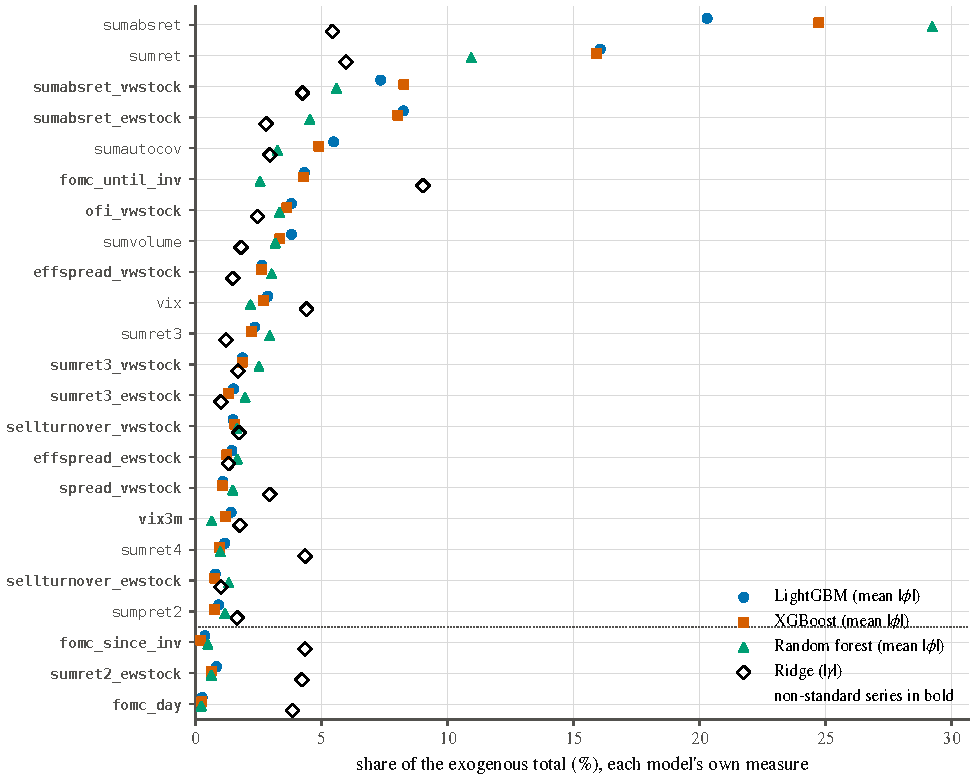
\includegraphics[width=\linewidth]{figures/fi_pooled/fip_rank.pdf}
\caption{Which exogenous series the models use. Each series' share of the exogenous attribution, pooled over the \rhfipNOrigins{} monthly origins: the tree ensembles' share of the mean absolute SHAP value (filled markers) and the ridge's share of the absolute standardized coefficients $|\gamma|$ (open diamonds). Rows: the 20 series with the largest mean share over the three tree ensembles, in that order, then (below the dotted line) the three series in the ridge's top ten that are not among them. Non-standard series are labeled in bold. The two measures differ; the figure compares rankings and shares, not magnitudes (Table~\ref{tab:rh_fip_shares}).}
\label{fig:rh_fip_rank}
\end{figure}

% Over time: non-standard share by year (trees, linear models) and the leading series by year (LightGBM, ridge)
% AUTO-GENERATED by writeup/make_rehaul_fi_pooled.py -- do not edit; re-run the script.
\providecommand{\ser}[2]{#2}\providecommand{\serx}[3]{#3}
\ifdefined\rhfipNOrigins\else% AUTO-GENERATED by writeup/make_rehaul_fi_pooled.py -- do not edit; re-run the script.
\providecommand{\ser}[2]{#2}\providecommand{\serx}[3]{#3}
% \rhfip... macros for writeup/rehaul/08_feature_importance.tex (results/tree_shap_w3000_2014start_fomcfix_2026-10-26, the
% FOMC-patched design, its linear reference inputs/fiw_gamma_fomcfix.npz; the window study's ...W... macros:
% results/fi_by_window_2014start_2026-10-22, pre-patch; the final pooled runs, W = 3,000 trading days).
\providecommand{\rhfipNOrigins}{}\renewcommand{\rhfipNOrigins}{126}  % monthly origins (re-estimations explained)
\providecommand{\rhfipNRows}{}\renewcommand{\rhfipNRows}{33{,}970}  % bars explained, every bar of the evaluation span
\providecommand{\rhfipOriginEvery}{}\renewcommand{\rhfipOriginEvery}{21}  % trading days between origins
\providecommand{\rhfipLastBlock}{}\renewcommand{\rhfipLastBlock}{18}  % trading days of the last origin's block
\providecommand{\rhfipFirstOrigin}{}\renewcommand{\rhfipFirstOrigin}{2~January~2014}  % first origin (10:00 bar)
\providecommand{\rhfipLastOrigin}{}\renewcommand{\rhfipLastOrigin}{5~April~2024}  % last origin
\providecommand{\rhfipLastDay}{}\renewcommand{\rhfipLastDay}{30~April~2024}  % day of the last bar explained
\providecommand{\rhfipWindowDays}{}\renewcommand{\rhfipWindowDays}{3{,}000}  % rolling window, trading days
\providecommand{\rhfipWindowBars}{}\renewcommand{\rhfipWindowBars}{39{,}000}  % rolling window, bars
\providecommand{\rhfipNCols}{}\renewcommand{\rhfipNCols}{564}  % predictors of the full set
\providecommand{\rhfipNGroups}{}\renewcommand{\rhfipNGroups}{48}  % predictor groups: 46 exogenous series + HAR components + calendar dummies
\providecommand{\rhfipNExog}{}\renewcommand{\rhfipNExog}{46}  % exogenous series
\providecommand{\rhfipNPerSeries}{}\renewcommand{\rhfipNPerSeries}{12}  % predictors per exogenous series: value and availability averages at six horizons
\providecommand{\rhfipNStd}{}\renewcommand{\rhfipNStd}{12}  % standard groups
\providecommand{\rhfipNNonStd}{}\renewcommand{\rhfipNNonStd}{36}  % non-standard series
\providecommand{\rhfipNStdExog}{}\renewcommand{\rhfipNStdExog}{10}  % standard exogenous series
\providecommand{\rhfipTuneLast}{}\renewcommand{\rhfipTuneLast}{31~December~2013}  % last day of the last tuning fold (fold 3)
\providecommand{\rhfipRidgePen}{}\renewcommand{\rhfipRidgePen}{\ensuremath{10^{3}}}
\providecommand{\rhfipLassoPen}{}\renewcommand{\rhfipLassoPen}{\ensuremath{10^{-4}}}
\providecommand{\rhfipEnetPen}{}\renewcommand{\rhfipEnetPen}{\ensuremath{10^{-3}}}
\providecommand{\rhfipHarPf}{}\renewcommand{\rhfipHarPf}{0.01}  % penalty factor, HAR block
\providecommand{\rhfipBootBlock}{}\renewcommand{\rhfipBootBlock}{12}  % bootstrap block, origins
\providecommand{\rhfipBootB}{}\renewcommand{\rhfipBootB}{2{,}000}
\providecommand{\rhfipCiLevel}{}\renewcommand{\rhfipCiLevel}{95}  % percentile intervals of both rules (RULE_shap.txt, RULE_fiw.txt)
\providecommand{\rhfipShapeMin}{}\renewcommand{\rhfipShapeMin}{0.5}  % M3 selection: share of at least this many percent
\providecommand{\rhfipTopN}{}\renewcommand{\rhfipTopN}{10}  % length of the top lists compared (m2_rank.csv top10_overlap)
\providecommand{\rhfipSlopeUnit}{}\renewcommand{\rhfipSlopeUnit}{1{,}000}  % trading days per unit of the window slope
\providecommand{\rhfipNMom}{}\renewcommand{\rhfipNMom}{seven}  % the futures' realized moments (standard)
\providecommand{\rhfipLgbmGateEq}{}\renewcommand{\rhfipLgbmGateEq}{126}  % origins bit-equal to the merged every-bar walk
\providecommand{\rhfipXgbGateEq}{}\renewcommand{\rhfipXgbGateEq}{126}  % origins bit-equal to the merged every-bar walk
\providecommand{\rhfipRfGateEq}{}\renewcommand{\rhfipRfGateEq}{126}  % origins bit-equal to the merged every-bar walk
\providecommand{\rhfipRfGateAtShap}{}\renewcommand{\rhfipRfGateAtShap}{126}  % forest origins the walk had written when the SHAP gate ran
\providecommand{\rhfipXgbAddMax}{}\renewcommand{\rhfipXgbAddMax}{\ensuremath{3.7\times 10^{-6}}}  % XGBoost additivity, float32
\providecommand{\rhfipXgbAddTol}{}\renewcommand{\rhfipXgbAddTol}{\ensuremath{10^{-5}}}
\providecommand{\rhfipAddMaxDouble}{}\renewcommand{\rhfipAddMaxDouble}{\ensuremath{5.1\times 10^{-14}}}
\providecommand{\rhfipLinGateMax}{}\renewcommand{\rhfipLinGateMax}{\ensuremath{4.4\times 10^{-16}}}  % linear replay vs walk forecasts, W = 3,000
\providecommand{\rhfipInterRows}{}\renewcommand{\rhfipInterRows}{1{,}008}  % M5 rows
\providecommand{\rhfipInterPerOrigin}{}\renewcommand{\rhfipInterPerOrigin}{8}  % M5 rows per origin
\providecommand{\rhfipFomcRows}{}\renewcommand{\rhfipFomcRows}{1{,}014}
\providecommand{\rhfipFomcDaysShap}{}\renewcommand{\rhfipFomcDaysShap}{78}  % FOMC statement days in the SHAP subset (M4; releases.parquet only)
\providecommand{\rhfipFomcDays}{}\renewcommand{\rhfipFomcDays}{81}  % scheduled FOMC statement days in the span (loader calendar)
\providecommand{\rhfipFomcDaysMissing}{}\renewcommand{\rhfipFomcDaysMissing}{3}  % statement days the SHAP subset leaves out (counted with the other days; the patched rerun's reducer keeps releases.parquet's days)
\providecommand{\rhfipNHolSessions}{}\renewcommand{\rhfipNHolSessions}{64}  % NYSE-holiday futures sessions among the explained bars (not scored in Table 1)
\providecommand{\rhfipNHolBars}{}\renewcommand{\rhfipNHolBars}{443}  % their regular-hours bars
\providecommand{\rhfipVixLo}{}\renewcommand{\rhfipVixLo}{13.96}
\providecommand{\rhfipVixHi}{}\renewcommand{\rhfipVixHi}{19.02}
\providecommand{\rhfipLgbmHar}{}\renewcommand{\rhfipLgbmHar}{51.7}
\providecommand{\rhfipLgbmHarLo}{}\renewcommand{\rhfipLgbmHarLo}{49.5}
\providecommand{\rhfipLgbmHarHi}{}\renewcommand{\rhfipLgbmHarHi}{53.7}
\providecommand{\rhfipLgbmMom}{}\renewcommand{\rhfipLgbmMom}{22.3}
\providecommand{\rhfipLgbmNs}{}\renewcommand{\rhfipLgbmNs}{21.8}
\providecommand{\rhfipLgbmNsLo}{}\renewcommand{\rhfipLgbmNsLo}{20.4}
\providecommand{\rhfipLgbmNsHi}{}\renewcommand{\rhfipLgbmNsHi}{23.4}
\providecommand{\rhfipLgbmNsEx}{}\renewcommand{\rhfipLgbmNsEx}{45.9}
\providecommand{\rhfipLgbmNsExLo}{}\renewcommand{\rhfipLgbmNsExLo}{44.2}
\providecommand{\rhfipLgbmNsExHi}{}\renewcommand{\rhfipLgbmNsExHi}{47.7}
\providecommand{\rhfipXgbHar}{}\renewcommand{\rhfipXgbHar}{52.0}
\providecommand{\rhfipXgbHarLo}{}\renewcommand{\rhfipXgbHarLo}{50.0}
\providecommand{\rhfipXgbHarHi}{}\renewcommand{\rhfipXgbHarHi}{53.8}
\providecommand{\rhfipXgbMom}{}\renewcommand{\rhfipXgbMom}{23.6}
\providecommand{\rhfipXgbNs}{}\renewcommand{\rhfipXgbNs}{20.6}
\providecommand{\rhfipXgbNsLo}{}\renewcommand{\rhfipXgbNsLo}{19.2}
\providecommand{\rhfipXgbNsHi}{}\renewcommand{\rhfipXgbNsHi}{22.2}
\providecommand{\rhfipXgbNsEx}{}\renewcommand{\rhfipXgbNsEx}{43.6}
\providecommand{\rhfipXgbNsExLo}{}\renewcommand{\rhfipXgbNsExLo}{41.8}
\providecommand{\rhfipXgbNsExHi}{}\renewcommand{\rhfipXgbNsExHi}{45.7}
\providecommand{\rhfipRfHar}{}\renewcommand{\rhfipRfHar}{57.6}
\providecommand{\rhfipRfHarLo}{}\renewcommand{\rhfipRfHarLo}{55.4}
\providecommand{\rhfipRfHarHi}{}\renewcommand{\rhfipRfHarHi}{59.6}
\providecommand{\rhfipRfMom}{}\renewcommand{\rhfipRfMom}{20.7}
\providecommand{\rhfipRfNs}{}\renewcommand{\rhfipRfNs}{18.6}
\providecommand{\rhfipRfNsLo}{}\renewcommand{\rhfipRfNsLo}{17.2}
\providecommand{\rhfipRfNsHi}{}\renewcommand{\rhfipRfNsHi}{20.3}
\providecommand{\rhfipRfNsEx}{}\renewcommand{\rhfipRfNsEx}{44.2}
\providecommand{\rhfipRfNsExLo}{}\renewcommand{\rhfipRfNsExLo}{42.1}
\providecommand{\rhfipRfNsExHi}{}\renewcommand{\rhfipRfNsExHi}{46.5}
\providecommand{\rhfipRidgeNsEx}{}\renewcommand{\rhfipRidgeNsEx}{68.8}
\providecommand{\rhfipRidgeNs}{}\renewcommand{\rhfipRidgeNs}{55.6}
\providecommand{\rhfipRidgeHar}{}\renewcommand{\rhfipRidgeHar}{17.5}
\providecommand{\rhfipLassoNsEx}{}\renewcommand{\rhfipLassoNsEx}{82.5}
\providecommand{\rhfipLassoNs}{}\renewcommand{\rhfipLassoNs}{76.5}
\providecommand{\rhfipLassoHar}{}\renewcommand{\rhfipLassoHar}{6.7}
\providecommand{\rhfipEnetNsEx}{}\renewcommand{\rhfipEnetNsEx}{60.0}
\providecommand{\rhfipEnetNs}{}\renewcommand{\rhfipEnetNs}{42.9}
\providecommand{\rhfipEnetHar}{}\renewcommand{\rhfipEnetHar}{26.4}
\providecommand{\rhfipHarMin}{}\renewcommand{\rhfipHarMin}{51.7}
\providecommand{\rhfipHarMax}{}\renewcommand{\rhfipHarMax}{57.6}
\providecommand{\rhfipMomMin}{}\renewcommand{\rhfipMomMin}{20.7}
\providecommand{\rhfipMomMax}{}\renewcommand{\rhfipMomMax}{23.6}
\providecommand{\rhfipNsExMin}{}\renewcommand{\rhfipNsExMin}{43.6}
\providecommand{\rhfipNsExMax}{}\renewcommand{\rhfipNsExMax}{45.9}
\providecommand{\rhfipSentMin}{}\renewcommand{\rhfipSentMin}{0.6}
\providecommand{\rhfipSentMax}{}\renewcommand{\rhfipSentMax}{0.8}
\providecommand{\rhfipVdMin}{}\renewcommand{\rhfipVdMin}{0.2}
\providecommand{\rhfipVdMax}{}\renewcommand{\rhfipVdMax}{0.3}
\providecommand{\rhfipFomcBucketMin}{}\renewcommand{\rhfipFomcBucketMin}{1.4}
\providecommand{\rhfipFomcBucketMax}{}\renewcommand{\rhfipFomcBucketMax}{2.3}
\providecommand{\rhfipVvixMin}{}\renewcommand{\rhfipVvixMin}{0.2}
\providecommand{\rhfipVvixMax}{}\renewcommand{\rhfipVvixMax}{0.3}
\providecommand{\rhfipVixThreeMMin}{}\renewcommand{\rhfipVixThreeMMin}{0.3}
\providecommand{\rhfipVixThreeMMax}{}\renewcommand{\rhfipVixThreeMMax}{0.7}
\providecommand{\rhfipFomcDayMin}{}\renewcommand{\rhfipFomcDayMin}{0.1}
\providecommand{\rhfipFomcDayMax}{}\renewcommand{\rhfipFomcDayMax}{0.1}
\providecommand{\rhfipNsOne}{}\renewcommand{\rhfipNsOne}{\ensuremath{\ser{sumabsret_vwstock}{\mathrm{RAV}^{\mathrm{VW}}}}}
\providecommand{\rhfipNsOneMin}{}\renewcommand{\rhfipNsOneMin}{2.4}
\providecommand{\rhfipNsOneMax}{}\renewcommand{\rhfipNsOneMax}{3.9}
\providecommand{\rhfipNsOneLgbm}{}\renewcommand{\rhfipNsOneLgbm}{3.5}
\providecommand{\rhfipNsOneXgb}{}\renewcommand{\rhfipNsOneXgb}{3.9}
\providecommand{\rhfipNsOneRf}{}\renewcommand{\rhfipNsOneRf}{2.4}
\providecommand{\rhfipNsTwo}{}\renewcommand{\rhfipNsTwo}{\ensuremath{\ser{sumabsret_ewstock}{\mathrm{RAV}^{\mathrm{EW}}}}}
\providecommand{\rhfipNsTwoMin}{}\renewcommand{\rhfipNsTwoMin}{1.9}
\providecommand{\rhfipNsTwoMax}{}\renewcommand{\rhfipNsTwoMax}{3.9}
\providecommand{\rhfipNsTwoLgbm}{}\renewcommand{\rhfipNsTwoLgbm}{3.9}
\providecommand{\rhfipNsTwoXgb}{}\renewcommand{\rhfipNsTwoXgb}{3.8}
\providecommand{\rhfipNsTwoRf}{}\renewcommand{\rhfipNsTwoRf}{1.9}
\providecommand{\rhfipNsThree}{}\renewcommand{\rhfipNsThree}{\ensuremath{\ser{fomc_until_inv}{\mathrm{FOMC}^{\mathrm{next}}}}}
\providecommand{\rhfipNsThreeMin}{}\renewcommand{\rhfipNsThreeMin}{1.1}
\providecommand{\rhfipNsThreeMax}{}\renewcommand{\rhfipNsThreeMax}{2.0}
\providecommand{\rhfipNsThreeLgbm}{}\renewcommand{\rhfipNsThreeLgbm}{2.0}
\providecommand{\rhfipNsThreeXgb}{}\renewcommand{\rhfipNsThreeXgb}{2.0}
\providecommand{\rhfipNsThreeRf}{}\renewcommand{\rhfipNsThreeRf}{1.1}
\providecommand{\rhfipNsFour}{}\renewcommand{\rhfipNsFour}{\ensuremath{\ser{ofi_vwstock}{\mathrm{OFI}^{\mathrm{VW}}}}}
\providecommand{\rhfipNsFourMin}{}\renewcommand{\rhfipNsFourMin}{1.4}
\providecommand{\rhfipNsFourMax}{}\renewcommand{\rhfipNsFourMax}{1.8}
\providecommand{\rhfipNsFourLgbm}{}\renewcommand{\rhfipNsFourLgbm}{1.8}
\providecommand{\rhfipNsFourXgb}{}\renewcommand{\rhfipNsFourXgb}{1.7}
\providecommand{\rhfipNsFourRf}{}\renewcommand{\rhfipNsFourRf}{1.4}
\providecommand{\rhfipNsFive}{}\renewcommand{\rhfipNsFive}{\ensuremath{\ser{effspread_vwstock}{\mathrm{EffSpread}^{\mathrm{VW}}}}}
\providecommand{\rhfipNsFiveMin}{}\renewcommand{\rhfipNsFiveMin}{1.2}
\providecommand{\rhfipNsFiveMax}{}\renewcommand{\rhfipNsFiveMax}{1.3}
\providecommand{\rhfipNsFiveLgbm}{}\renewcommand{\rhfipNsFiveLgbm}{1.2}
\providecommand{\rhfipNsFiveXgb}{}\renewcommand{\rhfipNsFiveXgb}{1.2}
\providecommand{\rhfipNsFiveRf}{}\renewcommand{\rhfipNsFiveRf}{1.3}
\providecommand{\rhfipTreeTopOne}{}\renewcommand{\rhfipTreeTopOne}{\ensuremath{\ser{sumabsret}{\mathrm{RAV}}}}
\providecommand{\rhfipTreeTopTwo}{}\renewcommand{\rhfipTreeTopTwo}{\ensuremath{\ser{sumret}{r}}}
\providecommand{\rhfipLgbmTopOneEx}{}\renewcommand{\rhfipLgbmTopOneEx}{20.3}
\providecommand{\rhfipXgbTopOneEx}{}\renewcommand{\rhfipXgbTopOneEx}{24.7}
\providecommand{\rhfipRfTopOneEx}{}\renewcommand{\rhfipRfTopOneEx}{29.2}
\providecommand{\rhfipRidgeTopOne}{}\renewcommand{\rhfipRidgeTopOne}{\ensuremath{\ser{fomc_until_inv}{\mathrm{FOMC}^{\mathrm{next}}}}}
\providecommand{\rhfipRidgeTopOneEx}{}\renewcommand{\rhfipRidgeTopOneEx}{9.0}
\providecommand{\rhfipLgbmNUsedAll}{}\renewcommand{\rhfipLgbmNUsedAll}{42}  % exogenous series split on at every origin
\providecommand{\rhfipLgbmUsedMin}{}\renewcommand{\rhfipLgbmUsedMin}{58}
\providecommand{\rhfipXgbNUsedAll}{}\renewcommand{\rhfipXgbNUsedAll}{43}  % exogenous series split on at every origin
\providecommand{\rhfipXgbUsedMin}{}\renewcommand{\rhfipXgbUsedMin}{72}
\providecommand{\rhfipRfNUsedAll}{}\renewcommand{\rhfipRfNUsedAll}{46}  % exogenous series split on at every origin
\providecommand{\rhfipRfUsedMin}{}\renewcommand{\rhfipRfUsedMin}{126}
\providecommand{\rhfipLgbmDRidge}{}\renewcommand{\rhfipLgbmDRidge}{\ensuremath{-}22.9}
\providecommand{\rhfipLgbmDRidgeLo}{}\renewcommand{\rhfipLgbmDRidgeLo}{\ensuremath{-}24.8}
\providecommand{\rhfipLgbmDRidgeHi}{}\renewcommand{\rhfipLgbmDRidgeHi}{\ensuremath{-}21.1}
\providecommand{\rhfipLgbmDLasso}{}\renewcommand{\rhfipLgbmDLasso}{\ensuremath{-}36.6}
\providecommand{\rhfipLgbmDLassoLo}{}\renewcommand{\rhfipLgbmDLassoLo}{\ensuremath{-}39.1}
\providecommand{\rhfipLgbmDLassoHi}{}\renewcommand{\rhfipLgbmDLassoHi}{\ensuremath{-}34.4}
\providecommand{\rhfipLgbmDEnet}{}\renewcommand{\rhfipLgbmDEnet}{\ensuremath{-}14.1}
\providecommand{\rhfipLgbmDEnetLo}{}\renewcommand{\rhfipLgbmDEnetLo}{\ensuremath{-}15.7}
\providecommand{\rhfipLgbmDEnetHi}{}\renewcommand{\rhfipLgbmDEnetHi}{\ensuremath{-}12.7}
\providecommand{\rhfipXgbDRidge}{}\renewcommand{\rhfipXgbDRidge}{\ensuremath{-}25.1}
\providecommand{\rhfipXgbDRidgeLo}{}\renewcommand{\rhfipXgbDRidgeLo}{\ensuremath{-}27.0}
\providecommand{\rhfipXgbDRidgeHi}{}\renewcommand{\rhfipXgbDRidgeHi}{\ensuremath{-}23.3}
\providecommand{\rhfipXgbDLasso}{}\renewcommand{\rhfipXgbDLasso}{\ensuremath{-}38.9}
\providecommand{\rhfipXgbDLassoLo}{}\renewcommand{\rhfipXgbDLassoLo}{\ensuremath{-}41.4}
\providecommand{\rhfipXgbDLassoHi}{}\renewcommand{\rhfipXgbDLassoHi}{\ensuremath{-}36.6}
\providecommand{\rhfipXgbDEnet}{}\renewcommand{\rhfipXgbDEnet}{\ensuremath{-}16.3}
\providecommand{\rhfipXgbDEnetLo}{}\renewcommand{\rhfipXgbDEnetLo}{\ensuremath{-}17.8}
\providecommand{\rhfipXgbDEnetHi}{}\renewcommand{\rhfipXgbDEnetHi}{\ensuremath{-}14.9}
\providecommand{\rhfipRfDRidge}{}\renewcommand{\rhfipRfDRidge}{\ensuremath{-}24.5}
\providecommand{\rhfipRfDRidgeLo}{}\renewcommand{\rhfipRfDRidgeLo}{\ensuremath{-}26.3}
\providecommand{\rhfipRfDRidgeHi}{}\renewcommand{\rhfipRfDRidgeHi}{\ensuremath{-}22.9}
\providecommand{\rhfipRfDLasso}{}\renewcommand{\rhfipRfDLasso}{\ensuremath{-}38.3}
\providecommand{\rhfipRfDLassoLo}{}\renewcommand{\rhfipRfDLassoLo}{\ensuremath{-}40.5}
\providecommand{\rhfipRfDLassoHi}{}\renewcommand{\rhfipRfDLassoHi}{\ensuremath{-}36.3}
\providecommand{\rhfipRfDEnet}{}\renewcommand{\rhfipRfDEnet}{\ensuremath{-}15.7}
\providecommand{\rhfipRfDEnetLo}{}\renewcommand{\rhfipRfDEnetLo}{\ensuremath{-}17.0}
\providecommand{\rhfipRfDEnetHi}{}\renewcommand{\rhfipRfDEnetHi}{\ensuremath{-}14.4}
\providecommand{\rhfipNDLess}{}\renewcommand{\rhfipNDLess}{27}  % tree-minus-linear D with the 95% interval below 0
\providecommand{\rhfipNDAll}{}\renewcommand{\rhfipNDAll}{27}  % D comparisons: 3 trees x 3 linear models x 3 denominators
\providecommand{\rhfipLgbmSpRidge}{}\renewcommand{\rhfipLgbmSpRidge}{0.57}
\providecommand{\rhfipLgbmTopRidge}{}\renewcommand{\rhfipLgbmTopRidge}{6}
\providecommand{\rhfipLgbmSpLasso}{}\renewcommand{\rhfipLgbmSpLasso}{0.49}
\providecommand{\rhfipLgbmTopLasso}{}\renewcommand{\rhfipLgbmTopLasso}{5}
\providecommand{\rhfipLgbmSpEnet}{}\renewcommand{\rhfipLgbmSpEnet}{0.66}
\providecommand{\rhfipLgbmTopEnet}{}\renewcommand{\rhfipLgbmTopEnet}{6}
\providecommand{\rhfipXgbSpRidge}{}\renewcommand{\rhfipXgbSpRidge}{0.55}
\providecommand{\rhfipXgbTopRidge}{}\renewcommand{\rhfipXgbTopRidge}{6}
\providecommand{\rhfipXgbSpLasso}{}\renewcommand{\rhfipXgbSpLasso}{0.47}
\providecommand{\rhfipXgbTopLasso}{}\renewcommand{\rhfipXgbTopLasso}{5}
\providecommand{\rhfipXgbSpEnet}{}\renewcommand{\rhfipXgbSpEnet}{0.63}
\providecommand{\rhfipXgbTopEnet}{}\renewcommand{\rhfipXgbTopEnet}{6}
\providecommand{\rhfipRfSpRidge}{}\renewcommand{\rhfipRfSpRidge}{0.53}
\providecommand{\rhfipRfTopRidge}{}\renewcommand{\rhfipRfTopRidge}{5}
\providecommand{\rhfipRfSpLasso}{}\renewcommand{\rhfipRfSpLasso}{0.43}
\providecommand{\rhfipRfTopLasso}{}\renewcommand{\rhfipRfTopLasso}{4}
\providecommand{\rhfipRfSpEnet}{}\renewcommand{\rhfipRfSpEnet}{0.60}
\providecommand{\rhfipRfTopEnet}{}\renewcommand{\rhfipRfTopEnet}{5}
\providecommand{\rhfipSpLgbmXgb}{}\renewcommand{\rhfipSpLgbmXgb}{0.99}
\providecommand{\rhfipSpLgbmRf}{}\renewcommand{\rhfipSpLgbmRf}{0.90}
\providecommand{\rhfipSpXgbRf}{}\renewcommand{\rhfipSpXgbRf}{0.89}
\providecommand{\rhfipRidgeRankFomcUntil}{}\renewcommand{\rhfipRidgeRankFomcUntil}{1}
\providecommand{\rhfipTreeRankFomcUntilMin}{}\renewcommand{\rhfipTreeRankFomcUntilMin}{6}
\providecommand{\rhfipTreeRankFomcUntilMax}{}\renewcommand{\rhfipTreeRankFomcUntilMax}{10}
\providecommand{\rhfipRidgeRankFomcDay}{}\renewcommand{\rhfipRidgeRankFomcDay}{9}
\providecommand{\rhfipTreeRankFomcDayMin}{}\renewcommand{\rhfipTreeRankFomcDayMin}{39}
\providecommand{\rhfipTreeRankFomcDayMax}{}\renewcommand{\rhfipTreeRankFomcDayMax}{43}
\providecommand{\rhfipFomcUntil}{}\renewcommand{\rhfipFomcUntil}{\ensuremath{\ser{fomc_until_inv}{\mathrm{FOMC}^{\mathrm{next}}}}}
\providecommand{\rhfipFomcDay}{}\renewcommand{\rhfipFomcDay}{\ensuremath{\ser{fomc_day}{\mathrm{FOMC}^{\mathrm{day}}}}}
\providecommand{\rhfipAbsVw}{}\renewcommand{\rhfipAbsVw}{\ensuremath{\ser{sumabsret_vwstock}{\mathrm{RAV}^{\mathrm{VW}}}}}
\providecommand{\rhfipOfi}{}\renewcommand{\rhfipOfi}{\ensuremath{\ser{ofi_vwstock}{\mathrm{OFI}^{\mathrm{VW}}}}}
\providecommand{\rhfipLgbmNeff}{}\renewcommand{\rhfipLgbmNeff}{11.0}
\providecommand{\rhfipLgbmNHalf}{}\renewcommand{\rhfipLgbmNHalf}{4}
\providecommand{\rhfipLgbmNEighty}{}\renewcommand{\rhfipLgbmNEighty}{13}
\providecommand{\rhfipXgbNeff}{}\renewcommand{\rhfipXgbNeff}{9.1}
\providecommand{\rhfipXgbNHalf}{}\renewcommand{\rhfipXgbNHalf}{4}
\providecommand{\rhfipXgbNEighty}{}\renewcommand{\rhfipXgbNEighty}{11}
\providecommand{\rhfipRfNeff}{}\renewcommand{\rhfipRfNeff}{8.9}
\providecommand{\rhfipRfNHalf}{}\renewcommand{\rhfipRfNHalf}{4}
\providecommand{\rhfipRfNEighty}{}\renewcommand{\rhfipRfNEighty}{16}
\providecommand{\rhfipRidgeNeff}{}\renewcommand{\rhfipRidgeNeff}{28.5}
\providecommand{\rhfipRidgeNHalf}{}\renewcommand{\rhfipRidgeNHalf}{11}
\providecommand{\rhfipRidgeNEighty}{}\renewcommand{\rhfipRidgeNEighty}{26}
\providecommand{\rhfipLassoNeff}{}\renewcommand{\rhfipLassoNeff}{5.1}
\providecommand{\rhfipLassoNHalf}{}\renewcommand{\rhfipLassoNHalf}{2}
\providecommand{\rhfipLassoNEighty}{}\renewcommand{\rhfipLassoNEighty}{11}
\providecommand{\rhfipEnetNeff}{}\renewcommand{\rhfipEnetNeff}{16.2}
\providecommand{\rhfipEnetNHalf}{}\renewcommand{\rhfipEnetNHalf}{6}
\providecommand{\rhfipEnetNEighty}{}\renewcommand{\rhfipEnetNEighty}{15}
\providecommand{\rhfipYearFirst}{}\renewcommand{\rhfipYearFirst}{2014}
\providecommand{\rhfipYearLast}{}\renewcommand{\rhfipYearLast}{2024}
\providecommand{\rhfipLgbmNsYearMin}{}\renewcommand{\rhfipLgbmNsYearMin}{18.1}
\providecommand{\rhfipLgbmNsYearMinYr}{}\renewcommand{\rhfipLgbmNsYearMinYr}{2021}
\providecommand{\rhfipLgbmNsYearMax}{}\renewcommand{\rhfipLgbmNsYearMax}{25.6}
\providecommand{\rhfipLgbmNsYearMaxYr}{}\renewcommand{\rhfipLgbmNsYearMaxYr}{2015}
\providecommand{\rhfipLgbmHarYearMax}{}\renewcommand{\rhfipLgbmHarYearMax}{57.4}
\providecommand{\rhfipLgbmHarYearMaxYr}{}\renewcommand{\rhfipLgbmHarYearMaxYr}{2021}
\providecommand{\rhfipLgbmHarYearMin}{}\renewcommand{\rhfipLgbmHarYearMin}{44.6}
\providecommand{\rhfipLgbmHarYearMinYr}{}\renewcommand{\rhfipLgbmHarYearMinYr}{2017}
\providecommand{\rhfipXgbNsYearMin}{}\renewcommand{\rhfipXgbNsYearMin}{17.2}
\providecommand{\rhfipXgbNsYearMinYr}{}\renewcommand{\rhfipXgbNsYearMinYr}{2021}
\providecommand{\rhfipXgbNsYearMax}{}\renewcommand{\rhfipXgbNsYearMax}{24.3}
\providecommand{\rhfipXgbNsYearMaxYr}{}\renewcommand{\rhfipXgbNsYearMaxYr}{2015}
\providecommand{\rhfipXgbHarYearMax}{}\renewcommand{\rhfipXgbHarYearMax}{57.0}
\providecommand{\rhfipXgbHarYearMaxYr}{}\renewcommand{\rhfipXgbHarYearMaxYr}{2021}
\providecommand{\rhfipXgbHarYearMin}{}\renewcommand{\rhfipXgbHarYearMin}{45.8}
\providecommand{\rhfipXgbHarYearMinYr}{}\renewcommand{\rhfipXgbHarYearMinYr}{2017}
\providecommand{\rhfipRfNsYearMin}{}\renewcommand{\rhfipRfNsYearMin}{15.2}
\providecommand{\rhfipRfNsYearMinYr}{}\renewcommand{\rhfipRfNsYearMinYr}{2021}
\providecommand{\rhfipRfNsYearMax}{}\renewcommand{\rhfipRfNsYearMax}{22.9}
\providecommand{\rhfipRfNsYearMaxYr}{}\renewcommand{\rhfipRfNsYearMaxYr}{2015}
\providecommand{\rhfipRfHarYearMax}{}\renewcommand{\rhfipRfHarYearMax}{62.3}
\providecommand{\rhfipRfHarYearMaxYr}{}\renewcommand{\rhfipRfHarYearMaxYr}{2019}
\providecommand{\rhfipRfHarYearMin}{}\renewcommand{\rhfipRfHarYearMin}{50.4}
\providecommand{\rhfipRfHarYearMinYr}{}\renewcommand{\rhfipRfHarYearMinYr}{2017}
\providecommand{\rhfipNsYearMinYr}{}\renewcommand{\rhfipNsYearMinYr}{2021}  % the year of every tree's lowest non-standard share
\providecommand{\rhfipDipFirst}{}\renewcommand{\rhfipDipFirst}{2018}  % first of the years in which every tree's non-standard share is below its pooled share
\providecommand{\rhfipDipLast}{}\renewcommand{\rhfipDipLast}{2022}
\providecommand{\rhfipRidgeNsExYearMin}{}\renewcommand{\rhfipRidgeNsExYearMin}{65.1}
\providecommand{\rhfipRidgeNsExYearMinYr}{}\renewcommand{\rhfipRidgeNsExYearMinYr}{2021}
\providecommand{\rhfipRidgeNsExYearMax}{}\renewcommand{\rhfipRidgeNsExYearMax}{72.4}
\providecommand{\rhfipRidgeNsExYearMaxYr}{}\renewcommand{\rhfipRidgeNsExYearMaxYr}{2017}
\providecommand{\rhfipLassoNsExYearMin}{}\renewcommand{\rhfipLassoNsExYearMin}{77.1}
\providecommand{\rhfipLassoNsExYearMinYr}{}\renewcommand{\rhfipLassoNsExYearMinYr}{2021}
\providecommand{\rhfipLassoNsExYearMax}{}\renewcommand{\rhfipLassoNsExYearMax}{87.1}
\providecommand{\rhfipLassoNsExYearMaxYr}{}\renewcommand{\rhfipLassoNsExYearMaxYr}{2017}
\providecommand{\rhfipEnetNsExYearMin}{}\renewcommand{\rhfipEnetNsExYearMin}{56.1}
\providecommand{\rhfipEnetNsExYearMinYr}{}\renewcommand{\rhfipEnetNsExYearMinYr}{2019}
\providecommand{\rhfipEnetNsExYearMax}{}\renewcommand{\rhfipEnetNsExYearMax}{65.2}
\providecommand{\rhfipEnetNsExYearMaxYr}{}\renewcommand{\rhfipEnetNsExYearMaxYr}{2014}
\providecommand{\rhfipLgbmNsExYearMin}{}\renewcommand{\rhfipLgbmNsExYearMin}{42.3}
\providecommand{\rhfipLgbmNsExYearMax}{}\renewcommand{\rhfipLgbmNsExYearMax}{50.1}
\providecommand{\rhfipXgbNsExYearMin}{}\renewcommand{\rhfipXgbNsExYearMin}{39.4}
\providecommand{\rhfipXgbNsExYearMax}{}\renewcommand{\rhfipXgbNsExYearMax}{48.9}
\providecommand{\rhfipRfNsExYearMin}{}\renewcommand{\rhfipRfNsExYearMin}{39.5}
\providecommand{\rhfipRfNsExYearMax}{}\renewcommand{\rhfipRfNsExYearMax}{50.9}
\providecommand{\rhfipLgbmNShape}{}\renewcommand{\rhfipLgbmNShape}{11}  % non-standard series at >= 0.5% (M3)
\providecommand{\rhfipLgbmNMono}{}\renewcommand{\rhfipLgbmNMono}{7}
\providecommand{\rhfipLgbmNIrr}{}\renewcommand{\rhfipLgbmNIrr}{3}
\providecommand{\rhfipLgbmNStep}{}\renewcommand{\rhfipLgbmNStep}{1}
\providecommand{\rhfipLgbmNFlat}{}\renewcommand{\rhfipLgbmNFlat}{0}
\providecommand{\rhfipLgbmNThresh}{}\renewcommand{\rhfipLgbmNThresh}{0}
\providecommand{\rhfipLgbmNU}{}\renewcommand{\rhfipLgbmNU}{0}
\providecommand{\rhfipLgbmNAsym}{}\renewcommand{\rhfipLgbmNAsym}{9}
\providecommand{\rhfipXgbNShape}{}\renewcommand{\rhfipXgbNShape}{10}  % non-standard series at >= 0.5% (M3)
\providecommand{\rhfipXgbNMono}{}\renewcommand{\rhfipXgbNMono}{5}
\providecommand{\rhfipXgbNIrr}{}\renewcommand{\rhfipXgbNIrr}{3}
\providecommand{\rhfipXgbNStep}{}\renewcommand{\rhfipXgbNStep}{0}
\providecommand{\rhfipXgbNFlat}{}\renewcommand{\rhfipXgbNFlat}{1}
\providecommand{\rhfipXgbNThresh}{}\renewcommand{\rhfipXgbNThresh}{1}
\providecommand{\rhfipXgbNU}{}\renewcommand{\rhfipXgbNU}{0}
\providecommand{\rhfipXgbNAsym}{}\renewcommand{\rhfipXgbNAsym}{8}
\providecommand{\rhfipRfNShape}{}\renewcommand{\rhfipRfNShape}{13}  % non-standard series at >= 0.5% (M3)
\providecommand{\rhfipRfNMono}{}\renewcommand{\rhfipRfNMono}{10}
\providecommand{\rhfipRfNIrr}{}\renewcommand{\rhfipRfNIrr}{3}
\providecommand{\rhfipRfNStep}{}\renewcommand{\rhfipRfNStep}{0}
\providecommand{\rhfipRfNFlat}{}\renewcommand{\rhfipRfNFlat}{0}
\providecommand{\rhfipRfNThresh}{}\renewcommand{\rhfipRfNThresh}{0}
\providecommand{\rhfipRfNU}{}\renewcommand{\rhfipRfNU}{0}
\providecommand{\rhfipRfNAsym}{}\renewcommand{\rhfipRfNAsym}{13}
\providecommand{\rhfipNUThreshAll}{}\renewcommand{\rhfipNUThreshAll}{1}  % U-shaped, inverted-U or threshold profiles in any tree
\providecommand{\rhfipAbsVwLgbmLo}{}\renewcommand{\rhfipAbsVwLgbmLo}{\ensuremath{-}1.4}
\providecommand{\rhfipAbsVwLgbmHi}{}\renewcommand{\rhfipAbsVwLgbmHi}{3.9}
\providecommand{\rhfipAbsVwXgbLo}{}\renewcommand{\rhfipAbsVwXgbLo}{\ensuremath{-}1.5}
\providecommand{\rhfipAbsVwXgbHi}{}\renewcommand{\rhfipAbsVwXgbHi}{4.3}
\providecommand{\rhfipAbsVwRfLo}{}\renewcommand{\rhfipAbsVwRfLo}{\ensuremath{-}0.9}
\providecommand{\rhfipAbsVwRfHi}{}\renewcommand{\rhfipAbsVwRfHi}{2.3}
\providecommand{\rhfipOfiLgbmLo}{}\renewcommand{\rhfipOfiLgbmLo}{0.8}
\providecommand{\rhfipOfiLgbmHi}{}\renewcommand{\rhfipOfiLgbmHi}{\ensuremath{-}1.1}
\providecommand{\rhfipOfiXgbLo}{}\renewcommand{\rhfipOfiXgbLo}{0.8}
\providecommand{\rhfipOfiXgbHi}{}\renewcommand{\rhfipOfiXgbHi}{\ensuremath{-}0.9}
\providecommand{\rhfipOfiRfLo}{}\renewcommand{\rhfipOfiRfLo}{0.8}
\providecommand{\rhfipOfiRfHi}{}\renewcommand{\rhfipOfiRfHi}{\ensuremath{-}0.7}
\providecommand{\rhfipUntilLgbmLo}{}\renewcommand{\rhfipUntilLgbmLo}{\ensuremath{-}0.3}
\providecommand{\rhfipUntilLgbmHi}{}\renewcommand{\rhfipUntilLgbmHi}{2.9}
\providecommand{\rhfipUntilXgbLo}{}\renewcommand{\rhfipUntilXgbLo}{0.2}
\providecommand{\rhfipUntilXgbHi}{}\renewcommand{\rhfipUntilXgbHi}{2.4}
\providecommand{\rhfipUntilRfLo}{}\renewcommand{\rhfipUntilRfLo}{\ensuremath{-}0.0}
\providecommand{\rhfipUntilRfHi}{}\renewcommand{\rhfipUntilRfHi}{1.5}
\providecommand{\rhfipUntilHorizon}{}\renewcommand{\rhfipUntilHorizon}{25}  % horizon of fomc_until_inv's dominant column
\providecommand{\rhfipUntilHorizonXgb}{}\renewcommand{\rhfipUntilHorizonXgb}{1}  % the same in XGBoost (differs from the other trees')
\providecommand{\rhfipBarFirst}{}\renewcommand{\rhfipBarFirst}{10:00}
\providecommand{\rhfipBarLast}{}\renewcommand{\rhfipBarLast}{16:00}
\providecommand{\rhfipBarPeakA}{}\renewcommand{\rhfipBarPeakA}{14:30}
\providecommand{\rhfipBarPeakB}{}\renewcommand{\rhfipBarPeakB}{15:00}
\providecommand{\rhfipNBars}{}\renewcommand{\rhfipNBars}{13}
\providecommand{\rhfipLgbmNsFomc}{}\renewcommand{\rhfipLgbmNsFomc}{42.6}
\providecommand{\rhfipLgbmNsOther}{}\renewcommand{\rhfipLgbmNsOther}{20.9}
\providecommand{\rhfipLgbmUntilFomc}{}\renewcommand{\rhfipLgbmUntilFomc}{25.4}
\providecommand{\rhfipLgbmUntilOther}{}\renewcommand{\rhfipLgbmUntilOther}{1.06}
\providecommand{\rhfipLgbmFomcBucketFomc}{}\renewcommand{\rhfipLgbmFomcBucketFomc}{27.3}
\providecommand{\rhfipLgbmFomcBucketOther}{}\renewcommand{\rhfipLgbmFomcBucketOther}{1.3}
\providecommand{\rhfipLgbmHarFomc}{}\renewcommand{\rhfipLgbmHarFomc}{39.2}
\providecommand{\rhfipLgbmHarOther}{}\renewcommand{\rhfipLgbmHarOther}{52.2}
\providecommand{\rhfipLgbmNsFirstBar}{}\renewcommand{\rhfipLgbmNsFirstBar}{23.9}
\providecommand{\rhfipLgbmNsLastBar}{}\renewcommand{\rhfipLgbmNsLastBar}{20.5}
\providecommand{\rhfipLgbmNsAftMin}{}\renewcommand{\rhfipLgbmNsAftMin}{24.3}
\providecommand{\rhfipLgbmNsAftMax}{}\renewcommand{\rhfipLgbmNsAftMax}{25.2}
\providecommand{\rhfipLgbmNsMidMin}{}\renewcommand{\rhfipLgbmNsMidMin}{20.1}
\providecommand{\rhfipLgbmNsMidMax}{}\renewcommand{\rhfipLgbmNsMidMax}{21.9}
\providecommand{\rhfipLgbmFomcBucketAft}{}\renewcommand{\rhfipLgbmFomcBucketAft}{5.5}
\providecommand{\rhfipLgbmFomcBucketOtherBars}{}\renewcommand{\rhfipLgbmFomcBucketOtherBars}{1.4}  % median FOMC-announcement share over the other 11 bars
\providecommand{\rhfipLgbmFomcDiff}{}\renewcommand{\rhfipLgbmFomcDiff}{\ensuremath{+}21.7}
\providecommand{\rhfipLgbmFomcDiffLo}{}\renewcommand{\rhfipLgbmFomcDiffLo}{\ensuremath{+}19.3}
\providecommand{\rhfipLgbmFomcDiffHi}{}\renewcommand{\rhfipLgbmFomcDiffHi}{\ensuremath{+}24.1}
\providecommand{\rhfipLgbmLateDiff}{}\renewcommand{\rhfipLgbmLateDiff}{\ensuremath{-}3.4}
\providecommand{\rhfipLgbmLateDiffLo}{}\renewcommand{\rhfipLgbmLateDiffLo}{\ensuremath{-}4.3}
\providecommand{\rhfipLgbmLateDiffHi}{}\renewcommand{\rhfipLgbmLateDiffHi}{\ensuremath{-}2.5}
\providecommand{\rhfipLgbmVixDiff}{}\renewcommand{\rhfipLgbmVixDiff}{\ensuremath{-}3.2}
\providecommand{\rhfipLgbmVixDiffLo}{}\renewcommand{\rhfipLgbmVixDiffLo}{\ensuremath{-}5.3}
\providecommand{\rhfipLgbmVixDiffHi}{}\renewcommand{\rhfipLgbmVixDiffHi}{\ensuremath{-}1.1}
\providecommand{\rhfipLgbmVixHar}{}\renewcommand{\rhfipLgbmVixHar}{\ensuremath{+}5.1}
\providecommand{\rhfipLgbmVixHarLo}{}\renewcommand{\rhfipLgbmVixHarLo}{\ensuremath{+}1.8}
\providecommand{\rhfipLgbmVixHarHi}{}\renewcommand{\rhfipLgbmVixHarHi}{\ensuremath{+}8.4}
\providecommand{\rhfipLgbmVixDiffEx}{}\renewcommand{\rhfipLgbmVixDiffEx}{\ensuremath{-}2.3}
\providecommand{\rhfipLgbmVixDiffExLo}{}\renewcommand{\rhfipLgbmVixDiffExLo}{\ensuremath{-}4.5}
\providecommand{\rhfipLgbmVixDiffExHi}{}\renewcommand{\rhfipLgbmVixDiffExHi}{\ensuremath{-}0.2}
\providecommand{\rhfipXgbNsFomc}{}\renewcommand{\rhfipXgbNsFomc}{41.1}
\providecommand{\rhfipXgbNsOther}{}\renewcommand{\rhfipXgbNsOther}{19.7}
\providecommand{\rhfipXgbUntilFomc}{}\renewcommand{\rhfipXgbUntilFomc}{23.9}
\providecommand{\rhfipXgbUntilOther}{}\renewcommand{\rhfipXgbUntilOther}{1.10}
\providecommand{\rhfipXgbFomcBucketFomc}{}\renewcommand{\rhfipXgbFomcBucketFomc}{25.6}
\providecommand{\rhfipXgbFomcBucketOther}{}\renewcommand{\rhfipXgbFomcBucketOther}{1.3}
\providecommand{\rhfipXgbHarFomc}{}\renewcommand{\rhfipXgbHarFomc}{39.1}
\providecommand{\rhfipXgbHarOther}{}\renewcommand{\rhfipXgbHarOther}{52.5}
\providecommand{\rhfipXgbNsFirstBar}{}\renewcommand{\rhfipXgbNsFirstBar}{22.5}
\providecommand{\rhfipXgbNsLastBar}{}\renewcommand{\rhfipXgbNsLastBar}{19.5}
\providecommand{\rhfipXgbNsAftMin}{}\renewcommand{\rhfipXgbNsAftMin}{23.5}
\providecommand{\rhfipXgbNsAftMax}{}\renewcommand{\rhfipXgbNsAftMax}{23.7}
\providecommand{\rhfipXgbNsMidMin}{}\renewcommand{\rhfipXgbNsMidMin}{19.1}
\providecommand{\rhfipXgbNsMidMax}{}\renewcommand{\rhfipXgbNsMidMax}{20.4}
\providecommand{\rhfipXgbFomcBucketAft}{}\renewcommand{\rhfipXgbFomcBucketAft}{5.8}
\providecommand{\rhfipXgbFomcBucketOtherBars}{}\renewcommand{\rhfipXgbFomcBucketOtherBars}{1.3}  % median FOMC-announcement share over the other 11 bars
\providecommand{\rhfipXgbFomcDiff}{}\renewcommand{\rhfipXgbFomcDiff}{\ensuremath{+}21.4}
\providecommand{\rhfipXgbFomcDiffLo}{}\renewcommand{\rhfipXgbFomcDiffLo}{\ensuremath{+}19.3}
\providecommand{\rhfipXgbFomcDiffHi}{}\renewcommand{\rhfipXgbFomcDiffHi}{\ensuremath{+}23.5}
\providecommand{\rhfipXgbLateDiff}{}\renewcommand{\rhfipXgbLateDiff}{\ensuremath{-}3.1}
\providecommand{\rhfipXgbLateDiffLo}{}\renewcommand{\rhfipXgbLateDiffLo}{\ensuremath{-}4.0}
\providecommand{\rhfipXgbLateDiffHi}{}\renewcommand{\rhfipXgbLateDiffHi}{\ensuremath{-}2.3}
\providecommand{\rhfipXgbVixDiff}{}\renewcommand{\rhfipXgbVixDiff}{\ensuremath{-}3.0}
\providecommand{\rhfipXgbVixDiffLo}{}\renewcommand{\rhfipXgbVixDiffLo}{\ensuremath{-}5.1}
\providecommand{\rhfipXgbVixDiffHi}{}\renewcommand{\rhfipXgbVixDiffHi}{\ensuremath{-}0.9}
\providecommand{\rhfipXgbVixHar}{}\renewcommand{\rhfipXgbVixHar}{\ensuremath{+}3.9}
\providecommand{\rhfipXgbVixHarLo}{}\renewcommand{\rhfipXgbVixHarLo}{\ensuremath{+}0.4}
\providecommand{\rhfipXgbVixHarHi}{}\renewcommand{\rhfipXgbVixHarHi}{\ensuremath{+}7.2}
\providecommand{\rhfipXgbVixDiffEx}{}\renewcommand{\rhfipXgbVixDiffEx}{\ensuremath{-}3.2}
\providecommand{\rhfipXgbVixDiffExLo}{}\renewcommand{\rhfipXgbVixDiffExLo}{\ensuremath{-}5.7}
\providecommand{\rhfipXgbVixDiffExHi}{}\renewcommand{\rhfipXgbVixDiffExHi}{\ensuremath{-}0.8}
\providecommand{\rhfipRfNsFomc}{}\renewcommand{\rhfipRfNsFomc}{28.9}
\providecommand{\rhfipRfNsOther}{}\renewcommand{\rhfipRfNsOther}{18.3}
\providecommand{\rhfipRfUntilFomc}{}\renewcommand{\rhfipRfUntilFomc}{12.4}
\providecommand{\rhfipRfFomcBucketFomc}{}\renewcommand{\rhfipRfFomcBucketFomc}{13.0}
\providecommand{\rhfipRfFomcBucketOther}{}\renewcommand{\rhfipRfFomcBucketOther}{1.0}
\providecommand{\rhfipRfHarFomc}{}\renewcommand{\rhfipRfHarFomc}{50.8}
\providecommand{\rhfipRfHarOther}{}\renewcommand{\rhfipRfHarOther}{57.9}
\providecommand{\rhfipRfNsFirstBar}{}\renewcommand{\rhfipRfNsFirstBar}{20.1}
\providecommand{\rhfipRfNsLastBar}{}\renewcommand{\rhfipRfNsLastBar}{17.8}
\providecommand{\rhfipRfNsAftMin}{}\renewcommand{\rhfipRfNsAftMin}{19.5}
\providecommand{\rhfipRfNsAftMax}{}\renewcommand{\rhfipRfNsAftMax}{19.9}
\providecommand{\rhfipRfNsMidMin}{}\renewcommand{\rhfipRfNsMidMin}{17.8}
\providecommand{\rhfipRfNsMidMax}{}\renewcommand{\rhfipRfNsMidMax}{18.6}
\providecommand{\rhfipRfFomcBucketAft}{}\renewcommand{\rhfipRfFomcBucketAft}{3.1}
\providecommand{\rhfipRfFomcBucketOtherBars}{}\renewcommand{\rhfipRfFomcBucketOtherBars}{1.0}  % median FOMC-announcement share over the other 11 bars
\providecommand{\rhfipRfFomcDiff}{}\renewcommand{\rhfipRfFomcDiff}{\ensuremath{+}10.6}
\providecommand{\rhfipRfFomcDiffLo}{}\renewcommand{\rhfipRfFomcDiffLo}{\ensuremath{+}8.3}
\providecommand{\rhfipRfFomcDiffHi}{}\renewcommand{\rhfipRfFomcDiffHi}{\ensuremath{+}13.1}
\providecommand{\rhfipRfLateDiff}{}\renewcommand{\rhfipRfLateDiff}{\ensuremath{-}2.3}
\providecommand{\rhfipRfLateDiffLo}{}\renewcommand{\rhfipRfLateDiffLo}{\ensuremath{-}3.1}
\providecommand{\rhfipRfLateDiffHi}{}\renewcommand{\rhfipRfLateDiffHi}{\ensuremath{-}1.6}
\providecommand{\rhfipRfVixDiff}{}\renewcommand{\rhfipRfVixDiff}{\ensuremath{-}3.3}
\providecommand{\rhfipRfVixDiffLo}{}\renewcommand{\rhfipRfVixDiffLo}{\ensuremath{-}5.1}
\providecommand{\rhfipRfVixDiffHi}{}\renewcommand{\rhfipRfVixDiffHi}{\ensuremath{-}1.4}
\providecommand{\rhfipRfVixHar}{}\renewcommand{\rhfipRfVixHar}{\ensuremath{+}4.2}
\providecommand{\rhfipRfVixHarLo}{}\renewcommand{\rhfipRfVixHarLo}{\ensuremath{+}1.0}
\providecommand{\rhfipRfVixHarHi}{}\renewcommand{\rhfipRfVixHarHi}{\ensuremath{+}7.3}
\providecommand{\rhfipRfVixDiffEx}{}\renewcommand{\rhfipRfVixDiffEx}{\ensuremath{-}3.7}
\providecommand{\rhfipRfVixDiffExLo}{}\renewcommand{\rhfipRfVixDiffExLo}{\ensuremath{-}6.3}
\providecommand{\rhfipRfVixDiffExHi}{}\renewcommand{\rhfipRfVixDiffExHi}{\ensuremath{-}1.2}
\providecommand{\rhfipLgbmInterVar}{}\renewcommand{\rhfipLgbmInterVar}{33.1}
\providecommand{\rhfipLgbmInterCol}{}\renewcommand{\rhfipLgbmInterCol}{45.3}
\providecommand{\rhfipLgbmInterNs}{}\renewcommand{\rhfipLgbmInterNs}{49.6}
\providecommand{\rhfipLgbmInterStd}{}\renewcommand{\rhfipLgbmInterStd}{26.8}
\providecommand{\rhfipLgbmInterStdEx}{}\renewcommand{\rhfipLgbmInterStdEx}{40.2}  % descriptive: standard exogenous series only (no HAR, no calendar)
\providecommand{\rhfipLgbmInterHar}{}\renewcommand{\rhfipLgbmInterHar}{17.1}
\providecommand{\rhfipLgbmInterWeakMin}{}\renewcommand{\rhfipLgbmInterWeakMin}{54}
\providecommand{\rhfipLgbmInterWeakMax}{}\renewcommand{\rhfipLgbmInterWeakMax}{66}
\providecommand{\rhfipLgbmPairOne}{}\renewcommand{\rhfipLgbmPairOne}{1.25}
\providecommand{\rhfipLgbmPairTwo}{}\renewcommand{\rhfipLgbmPairTwo}{0.86}
\providecommand{\rhfipLgbmCellHarHar}{}\renewcommand{\rhfipLgbmCellHarHar}{48.0}
\providecommand{\rhfipXgbInterVar}{}\renewcommand{\rhfipXgbInterVar}{30.9}
\providecommand{\rhfipXgbInterCol}{}\renewcommand{\rhfipXgbInterCol}{42.5}
\providecommand{\rhfipXgbInterNs}{}\renewcommand{\rhfipXgbInterNs}{45.7}
\providecommand{\rhfipXgbInterStd}{}\renewcommand{\rhfipXgbInterStd}{26.0}
\providecommand{\rhfipXgbInterStdEx}{}\renewcommand{\rhfipXgbInterStdEx}{37.8}  % descriptive: standard exogenous series only (no HAR, no calendar)
\providecommand{\rhfipXgbInterHar}{}\renewcommand{\rhfipXgbInterHar}{17.6}
\providecommand{\rhfipXgbInterWeakMin}{}\renewcommand{\rhfipXgbInterWeakMin}{54}
\providecommand{\rhfipXgbInterWeakMax}{}\renewcommand{\rhfipXgbInterWeakMax}{63}
\providecommand{\rhfipXgbPairOne}{}\renewcommand{\rhfipXgbPairOne}{1.23}
\providecommand{\rhfipXgbPairTwo}{}\renewcommand{\rhfipXgbPairTwo}{0.83}
\providecommand{\rhfipXgbCellHarHar}{}\renewcommand{\rhfipXgbCellHarHar}{47.4}
\providecommand{\rhfipPairOneA}{}\renewcommand{\rhfipPairOneA}{HAR components}
\providecommand{\rhfipPairOneB}{}\renewcommand{\rhfipPairOneB}{\ensuremath{\ser{sumabsret_vwstock}{\mathrm{RAV}^{\mathrm{VW}}}}}
\providecommand{\rhfipPairTwoA}{}\renewcommand{\rhfipPairTwoA}{HAR components}
\providecommand{\rhfipPairTwoB}{}\renewcommand{\rhfipPairTwoB}{\ensuremath{\ser{sumabsret_ewstock}{\mathrm{RAV}^{\mathrm{EW}}}}}
\providecommand{\rhfipLgbmPairsHar}{}\renewcommand{\rhfipLgbmPairsHar}{7}
\providecommand{\rhfipXgbPairsHar}{}\renewcommand{\rhfipXgbPairsHar}{7}
\providecommand{\rhfipWMin}{}\renewcommand{\rhfipWMin}{1{,}000}
\providecommand{\rhfipWMax}{}\renewcommand{\rhfipWMax}{3{,}500}
\providecommand{\rhfipNWindows}{}\renewcommand{\rhfipNWindows}{6}
\providecommand{\rhfipSOneMeasures}{}\renewcommand{\rhfipSOneMeasures}{105}  % measure x common-penalty fits of the window study (P1 and P2)
\providecommand{\rhfipSOneRises}{}\renewcommand{\rhfipSOneRises}{0}  % ... of which rise with W
\providecommand{\rhfipSOneFalls}{}\renewcommand{\rhfipSOneFalls}{102}
\providecommand{\rhfipSOneFlat}{}\renewcommand{\rhfipSOneFlat}{3}
\providecommand{\rhfipSOneNotSupported}{}\renewcommand{\rhfipSOneNotSupported}{14}  % common-penalty verdicts NOT SUPPORTED
\providecommand{\rhfipSOneVerdicts}{}\renewcommand{\rhfipSOneVerdicts}{14}
\providecommand{\rhfipRidgeNeffWMin}{}\renewcommand{\rhfipRidgeNeffWMin}{29.2}
\providecommand{\rhfipRidgeNeffWMain}{}\renewcommand{\rhfipRidgeNeffWMain}{29.2}
\providecommand{\rhfipRidgeNeffWMax}{}\renewcommand{\rhfipRidgeNeffWMax}{28.2}
\providecommand{\rhfipRidgeNeffSlope}{}\renewcommand{\rhfipRidgeNeffSlope}{\ensuremath{-}0.10}
\providecommand{\rhfipRidgeNeffSlopeLo}{}\renewcommand{\rhfipRidgeNeffSlopeLo}{\ensuremath{-}0.25}
\providecommand{\rhfipRidgeNeffSlopeHi}{}\renewcommand{\rhfipRidgeNeffSlopeHi}{0.12}
\providecommand{\rhfipRidgeSOneLoNeffWMin}{}\renewcommand{\rhfipRidgeSOneLoNeffWMin}{33.9}
\providecommand{\rhfipRidgeSOneLoNeffWMax}{}\renewcommand{\rhfipRidgeSOneLoNeffWMax}{28.2}
\providecommand{\rhfipRidgeSOneHiNeffWMin}{}\renewcommand{\rhfipRidgeSOneHiNeffWMin}{29.2}
\providecommand{\rhfipRidgeSOneHiNeffWMax}{}\renewcommand{\rhfipRidgeSOneHiNeffWMax}{23.5}
\providecommand{\rhfipLassoSOneVWMin}{}\renewcommand{\rhfipLassoSOneVWMin}{38.7}
\providecommand{\rhfipLassoSOneVWMax}{}\renewcommand{\rhfipLassoSOneVWMax}{31.9}
\providecommand{\rhfipLassoSOneCWMin}{}\renewcommand{\rhfipLassoSOneCWMin}{213.3}
\providecommand{\rhfipLassoSOneCWMax}{}\renewcommand{\rhfipLassoSOneCWMax}{177.5}
\providecommand{\rhfipLassoWalkVWMin}{}\renewcommand{\rhfipLassoWalkVWMin}{38.8}
\providecommand{\rhfipLassoWalkVWMax}{}\renewcommand{\rhfipLassoWalkVWMax}{41.9}
\providecommand{\rhfipLassoSOneLo}{}\renewcommand{\rhfipLassoSOneLo}{\ensuremath{10^{-3}}}
\providecommand{\rhfipRidgeSOneLo}{}\renewcommand{\rhfipRidgeSOneLo}{\ensuremath{10^{3}}}
\providecommand{\rhfipRidgeSOneHi}{}\renewcommand{\rhfipRidgeSOneHi}{\ensuremath{10^{4}}}
\providecommand{\rhfipEnetPenWMin}{}\renewcommand{\rhfipEnetPenWMin}{\ensuremath{10^{-2}}}
\providecommand{\rhfipEnetPenWNext}{}\renewcommand{\rhfipEnetPenWNext}{\ensuremath{10^{-3}}}
\providecommand{\rhfipWNext}{}\renewcommand{\rhfipWNext}{1{,}500}
\providecommand{\rhfipRidgePOneWalk}{}\renewcommand{\rhfipRidgePOneWalk}{not supported}
\providecommand{\rhfipRidgePTwoWalk}{}\renewcommand{\rhfipRidgePTwoWalk}{not supported}
\providecommand{\rhfipLassoPOneWalk}{}\renewcommand{\rhfipLassoPOneWalk}{partly}
\providecommand{\rhfipLassoPTwoWalk}{}\renewcommand{\rhfipLassoPTwoWalk}{not supported}
\providecommand{\rhfipEnetPOneWalk}{}\renewcommand{\rhfipEnetPOneWalk}{supported}
\providecommand{\rhfipEnetPTwoWalk}{}\renewcommand{\rhfipEnetPTwoWalk}{supported}
\fi
\begin{figure}[tbp]
\centering
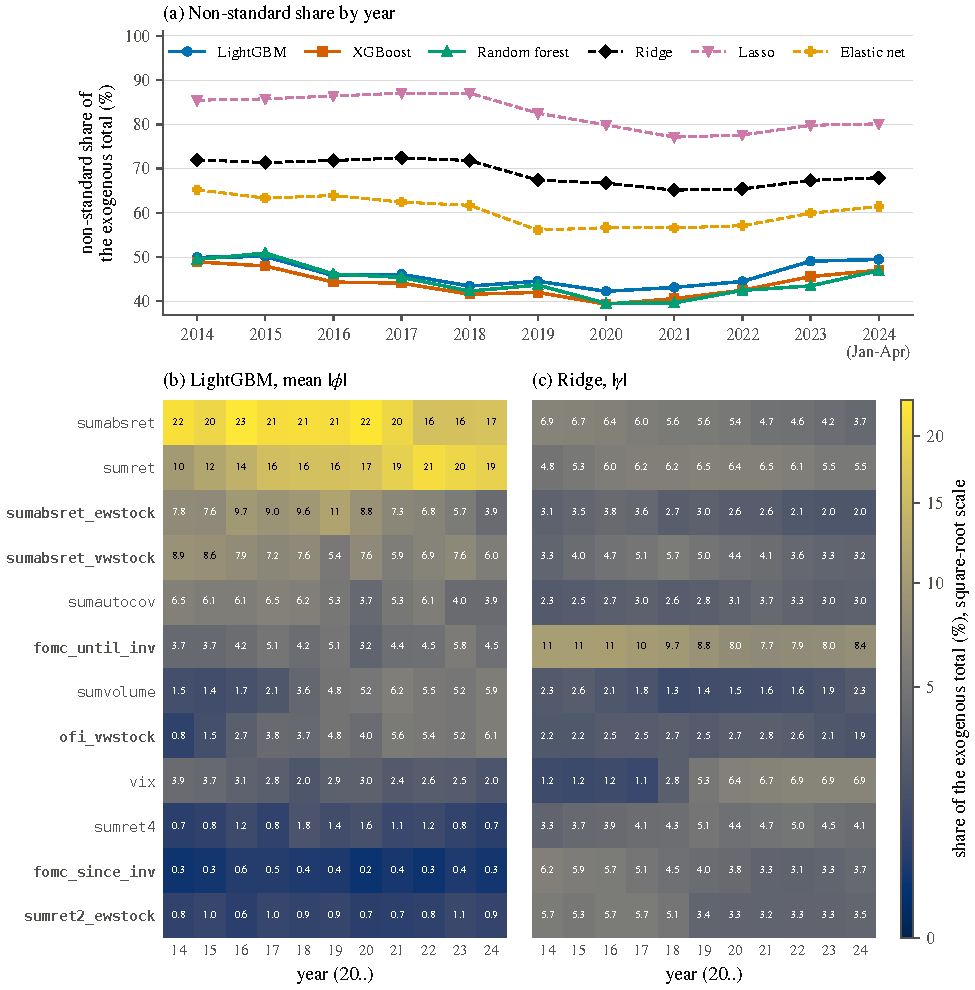
\includegraphics[width=\linewidth]{figures/fi_pooled/fip_time.pdf}
\caption{Variable importance over time. (a) The \rhfipNNonStd{} non-standard series' share of each model's exogenous attribution by calendar year: tree ensembles (solid) by the year of the forecast bar, linear models (dashed) by the year of the origin whose coefficients enter. (b), (c) The share of the exogenous total by year for the leading series of LightGBM and of the ridge (the union of each model's eight largest pooled shares; non-standard series in bold), on one square-root color scale. Shares of each model's own measure: mean absolute SHAP value for the trees, $|\gamma|$ for the linear models. The linear shares by year are computed here from the coefficients at the origins (descriptive). \rhfipYearLast{} covers January to April.}
\label{fig:rh_fip_time}
\end{figure}


% ---------------------------------------------------------------------------------------------------------------------
% 2026-10-26 (integration, JFEc): moved from 08_feature_importance.tex, "Only sometimes, or conditionally?".
% AUDIT results-9 (open, generator change flagged to NUMBERS): \rhfipFomcDays prints 78 FOMC statement days, but the
% span holds 81 scheduled statements. The SHAP reducer (results/tree_shap_w3000_2014start_2026-10-23/code/
% shap_reduce.py:662-670) builds the FOMC-day subset from data/releases.parquet ('fomc release' > 0), which lacks the
% three statements the loader adds (src/data/loading.py FOMC_MISSING_STATEMENTS: 2023-12-13, 2024-01-31, 2024-03-20;
% Data section), so their 39 bars count as other days. Fix: build the subset from the loader's calendar, recompute
% \rhfipFomcDays, \rhfipFomcRows and the ...NsFomc / ...NsOther / ...UntilFomc / ...UntilOther / ...FomcDiff macros
% (writeup/make_rehaul_fi_pooled.py). The tree SHAP study is to be rerun on the FOMC-patched design anyway (D13).
\subsection{Variable importance: conditional shares}
\label{app:rh_fi_cond}
\begin{itemize}
\item \textbf{Only sometimes, or conditionally?} (Figure~\ref{fig:rh_fip_cond}). The trees split on most series at
  every origin (\rhfipLgbmNUsedAll, \rhfipXgbNUsedAll{} and \rhfipRfNUsedAll{} of the \rhfipNExog); what changes with
  the conditions is how much the series move the forecast.
  \begin{itemize}
  \item FOMC statement days (\rhfipFomcDays{} days in the span): the non-standard share is \rhfipLgbmNsFomc,
    \rhfipXgbNsFomc{} and \rhfipRfNsFomc\% of the total, against \rhfipLgbmNsOther, \rhfipXgbNsOther{} and
    \rhfipRfNsOther\% on other days (differences \rhfipLgbmFomcDiff{} [\rhfipLgbmFomcDiffLo, \rhfipLgbmFomcDiffHi],
    \rhfipXgbFomcDiff{} [\rhfipXgbFomcDiffLo, \rhfipXgbFomcDiffHi] and \rhfipRfFomcDiff{} [\rhfipRfFomcDiffLo,
    \rhfipRfFomcDiffHi] percentage points). Almost all of it is \rhfipFomcUntil: \rhfipLgbmUntilFomc,
    \rhfipXgbUntilFomc{} and \rhfipRfUntilFomc\% of the total on statement days, against \rhfipLgbmUntilOther{} and
    \rhfipXgbUntilOther\% on other days (LightGBM, XGBoost).
  \item Bar of the day: the non-standard share is highest at the first bar, \rhfipBarFirst{} (\rhfipLgbmNsFirstBar,
    \rhfipXgbNsFirstBar, \rhfipRfNsFirstBar\%), and at \rhfipBarPeakA{} and \rhfipBarPeakB{} (LightGBM
    \rhfipLgbmNsAftMin--\rhfipLgbmNsAftMax\%), the bars where the FOMC calendar's share peaks (LightGBM
    \rhfipLgbmFomcBucketAft\%, against a median of \rhfipLgbmFomcBucketOtherBars\% over the other bars). It is lower
    at the last bar: \rhfipBarLast{} minus \rhfipBarFirst{} \rhfipLgbmLateDiff{} [\rhfipLgbmLateDiffLo,
    \rhfipLgbmLateDiffHi], \rhfipXgbLateDiff{} [\rhfipXgbLateDiffLo, \rhfipXgbLateDiffHi] and \rhfipRfLateDiff{}
    [\rhfipRfLateDiffLo, \rhfipRfLateDiffHi] percentage points.
  \item Volatility regime (tercile of the VIX close before the origin): the non-standard share is lower in the
    high-VIX tercile than in the low one, \rhfipLgbmVixDiff{} [\rhfipLgbmVixDiffLo, \rhfipLgbmVixDiffHi],
    \rhfipXgbVixDiff{} [\rhfipXgbVixDiffLo, \rhfipXgbVixDiffHi] and \rhfipRfVixDiff{} [\rhfipRfVixDiffLo,
    \rhfipRfVixDiffHi] percentage points of the total, and the HAR components gain instead (\rhfipLgbmVixHar,
    \rhfipXgbVixHar, \rhfipRfVixHar). As a share of the exogenous total the drop is clear for XGBoost and the forest
    and not for LightGBM (\rhfipLgbmVixDiffEx{} [\rhfipLgbmVixDiffExLo, \rhfipLgbmVixDiffExHi]).
  \end{itemize}
\end{itemize}
% Conditional: by bar of the day, FOMC statement days, VIX tercile
% AUTO-GENERATED by writeup/make_rehaul_fi_pooled.py -- do not edit; re-run the script.
\providecommand{\ser}[2]{#2}\providecommand{\serx}[3]{#3}
\ifdefined\rhfipNOrigins\else% AUTO-GENERATED by writeup/make_rehaul_fi_pooled.py -- do not edit; re-run the script.
\providecommand{\ser}[2]{#2}\providecommand{\serx}[3]{#3}
% \rhfip... macros for writeup/rehaul/08_feature_importance.tex (results/tree_shap_w3000_2014start_fomcfix_2026-10-26, the
% FOMC-patched design, its linear reference inputs/fiw_gamma_fomcfix.npz; the window study's ...W... macros:
% results/fi_by_window_2014start_2026-10-22, pre-patch; the final pooled runs, W = 3,000 trading days).
\providecommand{\rhfipNOrigins}{}\renewcommand{\rhfipNOrigins}{126}  % monthly origins (re-estimations explained)
\providecommand{\rhfipNRows}{}\renewcommand{\rhfipNRows}{33{,}970}  % bars explained, every bar of the evaluation span
\providecommand{\rhfipOriginEvery}{}\renewcommand{\rhfipOriginEvery}{21}  % trading days between origins
\providecommand{\rhfipLastBlock}{}\renewcommand{\rhfipLastBlock}{18}  % trading days of the last origin's block
\providecommand{\rhfipFirstOrigin}{}\renewcommand{\rhfipFirstOrigin}{2~January~2014}  % first origin (10:00 bar)
\providecommand{\rhfipLastOrigin}{}\renewcommand{\rhfipLastOrigin}{5~April~2024}  % last origin
\providecommand{\rhfipLastDay}{}\renewcommand{\rhfipLastDay}{30~April~2024}  % day of the last bar explained
\providecommand{\rhfipWindowDays}{}\renewcommand{\rhfipWindowDays}{3{,}000}  % rolling window, trading days
\providecommand{\rhfipWindowBars}{}\renewcommand{\rhfipWindowBars}{39{,}000}  % rolling window, bars
\providecommand{\rhfipNCols}{}\renewcommand{\rhfipNCols}{564}  % predictors of the full set
\providecommand{\rhfipNGroups}{}\renewcommand{\rhfipNGroups}{48}  % predictor groups: 46 exogenous series + HAR components + calendar dummies
\providecommand{\rhfipNExog}{}\renewcommand{\rhfipNExog}{46}  % exogenous series
\providecommand{\rhfipNPerSeries}{}\renewcommand{\rhfipNPerSeries}{12}  % predictors per exogenous series: value and availability averages at six horizons
\providecommand{\rhfipNStd}{}\renewcommand{\rhfipNStd}{12}  % standard groups
\providecommand{\rhfipNNonStd}{}\renewcommand{\rhfipNNonStd}{36}  % non-standard series
\providecommand{\rhfipNStdExog}{}\renewcommand{\rhfipNStdExog}{10}  % standard exogenous series
\providecommand{\rhfipTuneLast}{}\renewcommand{\rhfipTuneLast}{31~December~2013}  % last day of the last tuning fold (fold 3)
\providecommand{\rhfipRidgePen}{}\renewcommand{\rhfipRidgePen}{\ensuremath{10^{3}}}
\providecommand{\rhfipLassoPen}{}\renewcommand{\rhfipLassoPen}{\ensuremath{10^{-4}}}
\providecommand{\rhfipEnetPen}{}\renewcommand{\rhfipEnetPen}{\ensuremath{10^{-3}}}
\providecommand{\rhfipHarPf}{}\renewcommand{\rhfipHarPf}{0.01}  % penalty factor, HAR block
\providecommand{\rhfipBootBlock}{}\renewcommand{\rhfipBootBlock}{12}  % bootstrap block, origins
\providecommand{\rhfipBootB}{}\renewcommand{\rhfipBootB}{2{,}000}
\providecommand{\rhfipCiLevel}{}\renewcommand{\rhfipCiLevel}{95}  % percentile intervals of both rules (RULE_shap.txt, RULE_fiw.txt)
\providecommand{\rhfipShapeMin}{}\renewcommand{\rhfipShapeMin}{0.5}  % M3 selection: share of at least this many percent
\providecommand{\rhfipTopN}{}\renewcommand{\rhfipTopN}{10}  % length of the top lists compared (m2_rank.csv top10_overlap)
\providecommand{\rhfipSlopeUnit}{}\renewcommand{\rhfipSlopeUnit}{1{,}000}  % trading days per unit of the window slope
\providecommand{\rhfipNMom}{}\renewcommand{\rhfipNMom}{seven}  % the futures' realized moments (standard)
\providecommand{\rhfipLgbmGateEq}{}\renewcommand{\rhfipLgbmGateEq}{126}  % origins bit-equal to the merged every-bar walk
\providecommand{\rhfipXgbGateEq}{}\renewcommand{\rhfipXgbGateEq}{126}  % origins bit-equal to the merged every-bar walk
\providecommand{\rhfipRfGateEq}{}\renewcommand{\rhfipRfGateEq}{126}  % origins bit-equal to the merged every-bar walk
\providecommand{\rhfipRfGateAtShap}{}\renewcommand{\rhfipRfGateAtShap}{126}  % forest origins the walk had written when the SHAP gate ran
\providecommand{\rhfipXgbAddMax}{}\renewcommand{\rhfipXgbAddMax}{\ensuremath{3.7\times 10^{-6}}}  % XGBoost additivity, float32
\providecommand{\rhfipXgbAddTol}{}\renewcommand{\rhfipXgbAddTol}{\ensuremath{10^{-5}}}
\providecommand{\rhfipAddMaxDouble}{}\renewcommand{\rhfipAddMaxDouble}{\ensuremath{5.1\times 10^{-14}}}
\providecommand{\rhfipLinGateMax}{}\renewcommand{\rhfipLinGateMax}{\ensuremath{4.4\times 10^{-16}}}  % linear replay vs walk forecasts, W = 3,000
\providecommand{\rhfipInterRows}{}\renewcommand{\rhfipInterRows}{1{,}008}  % M5 rows
\providecommand{\rhfipInterPerOrigin}{}\renewcommand{\rhfipInterPerOrigin}{8}  % M5 rows per origin
\providecommand{\rhfipFomcRows}{}\renewcommand{\rhfipFomcRows}{1{,}014}
\providecommand{\rhfipFomcDaysShap}{}\renewcommand{\rhfipFomcDaysShap}{78}  % FOMC statement days in the SHAP subset (M4; releases.parquet only)
\providecommand{\rhfipFomcDays}{}\renewcommand{\rhfipFomcDays}{81}  % scheduled FOMC statement days in the span (loader calendar)
\providecommand{\rhfipFomcDaysMissing}{}\renewcommand{\rhfipFomcDaysMissing}{3}  % statement days the SHAP subset leaves out (counted with the other days; the patched rerun's reducer keeps releases.parquet's days)
\providecommand{\rhfipNHolSessions}{}\renewcommand{\rhfipNHolSessions}{64}  % NYSE-holiday futures sessions among the explained bars (not scored in Table 1)
\providecommand{\rhfipNHolBars}{}\renewcommand{\rhfipNHolBars}{443}  % their regular-hours bars
\providecommand{\rhfipVixLo}{}\renewcommand{\rhfipVixLo}{13.96}
\providecommand{\rhfipVixHi}{}\renewcommand{\rhfipVixHi}{19.02}
\providecommand{\rhfipLgbmHar}{}\renewcommand{\rhfipLgbmHar}{51.7}
\providecommand{\rhfipLgbmHarLo}{}\renewcommand{\rhfipLgbmHarLo}{49.5}
\providecommand{\rhfipLgbmHarHi}{}\renewcommand{\rhfipLgbmHarHi}{53.7}
\providecommand{\rhfipLgbmMom}{}\renewcommand{\rhfipLgbmMom}{22.3}
\providecommand{\rhfipLgbmNs}{}\renewcommand{\rhfipLgbmNs}{21.8}
\providecommand{\rhfipLgbmNsLo}{}\renewcommand{\rhfipLgbmNsLo}{20.4}
\providecommand{\rhfipLgbmNsHi}{}\renewcommand{\rhfipLgbmNsHi}{23.4}
\providecommand{\rhfipLgbmNsEx}{}\renewcommand{\rhfipLgbmNsEx}{45.9}
\providecommand{\rhfipLgbmNsExLo}{}\renewcommand{\rhfipLgbmNsExLo}{44.2}
\providecommand{\rhfipLgbmNsExHi}{}\renewcommand{\rhfipLgbmNsExHi}{47.7}
\providecommand{\rhfipXgbHar}{}\renewcommand{\rhfipXgbHar}{52.0}
\providecommand{\rhfipXgbHarLo}{}\renewcommand{\rhfipXgbHarLo}{50.0}
\providecommand{\rhfipXgbHarHi}{}\renewcommand{\rhfipXgbHarHi}{53.8}
\providecommand{\rhfipXgbMom}{}\renewcommand{\rhfipXgbMom}{23.6}
\providecommand{\rhfipXgbNs}{}\renewcommand{\rhfipXgbNs}{20.6}
\providecommand{\rhfipXgbNsLo}{}\renewcommand{\rhfipXgbNsLo}{19.2}
\providecommand{\rhfipXgbNsHi}{}\renewcommand{\rhfipXgbNsHi}{22.2}
\providecommand{\rhfipXgbNsEx}{}\renewcommand{\rhfipXgbNsEx}{43.6}
\providecommand{\rhfipXgbNsExLo}{}\renewcommand{\rhfipXgbNsExLo}{41.8}
\providecommand{\rhfipXgbNsExHi}{}\renewcommand{\rhfipXgbNsExHi}{45.7}
\providecommand{\rhfipRfHar}{}\renewcommand{\rhfipRfHar}{57.6}
\providecommand{\rhfipRfHarLo}{}\renewcommand{\rhfipRfHarLo}{55.4}
\providecommand{\rhfipRfHarHi}{}\renewcommand{\rhfipRfHarHi}{59.6}
\providecommand{\rhfipRfMom}{}\renewcommand{\rhfipRfMom}{20.7}
\providecommand{\rhfipRfNs}{}\renewcommand{\rhfipRfNs}{18.6}
\providecommand{\rhfipRfNsLo}{}\renewcommand{\rhfipRfNsLo}{17.2}
\providecommand{\rhfipRfNsHi}{}\renewcommand{\rhfipRfNsHi}{20.3}
\providecommand{\rhfipRfNsEx}{}\renewcommand{\rhfipRfNsEx}{44.2}
\providecommand{\rhfipRfNsExLo}{}\renewcommand{\rhfipRfNsExLo}{42.1}
\providecommand{\rhfipRfNsExHi}{}\renewcommand{\rhfipRfNsExHi}{46.5}
\providecommand{\rhfipRidgeNsEx}{}\renewcommand{\rhfipRidgeNsEx}{68.8}
\providecommand{\rhfipRidgeNs}{}\renewcommand{\rhfipRidgeNs}{55.6}
\providecommand{\rhfipRidgeHar}{}\renewcommand{\rhfipRidgeHar}{17.5}
\providecommand{\rhfipLassoNsEx}{}\renewcommand{\rhfipLassoNsEx}{82.5}
\providecommand{\rhfipLassoNs}{}\renewcommand{\rhfipLassoNs}{76.5}
\providecommand{\rhfipLassoHar}{}\renewcommand{\rhfipLassoHar}{6.7}
\providecommand{\rhfipEnetNsEx}{}\renewcommand{\rhfipEnetNsEx}{60.0}
\providecommand{\rhfipEnetNs}{}\renewcommand{\rhfipEnetNs}{42.9}
\providecommand{\rhfipEnetHar}{}\renewcommand{\rhfipEnetHar}{26.4}
\providecommand{\rhfipHarMin}{}\renewcommand{\rhfipHarMin}{51.7}
\providecommand{\rhfipHarMax}{}\renewcommand{\rhfipHarMax}{57.6}
\providecommand{\rhfipMomMin}{}\renewcommand{\rhfipMomMin}{20.7}
\providecommand{\rhfipMomMax}{}\renewcommand{\rhfipMomMax}{23.6}
\providecommand{\rhfipNsExMin}{}\renewcommand{\rhfipNsExMin}{43.6}
\providecommand{\rhfipNsExMax}{}\renewcommand{\rhfipNsExMax}{45.9}
\providecommand{\rhfipSentMin}{}\renewcommand{\rhfipSentMin}{0.6}
\providecommand{\rhfipSentMax}{}\renewcommand{\rhfipSentMax}{0.8}
\providecommand{\rhfipVdMin}{}\renewcommand{\rhfipVdMin}{0.2}
\providecommand{\rhfipVdMax}{}\renewcommand{\rhfipVdMax}{0.3}
\providecommand{\rhfipFomcBucketMin}{}\renewcommand{\rhfipFomcBucketMin}{1.4}
\providecommand{\rhfipFomcBucketMax}{}\renewcommand{\rhfipFomcBucketMax}{2.3}
\providecommand{\rhfipVvixMin}{}\renewcommand{\rhfipVvixMin}{0.2}
\providecommand{\rhfipVvixMax}{}\renewcommand{\rhfipVvixMax}{0.3}
\providecommand{\rhfipVixThreeMMin}{}\renewcommand{\rhfipVixThreeMMin}{0.3}
\providecommand{\rhfipVixThreeMMax}{}\renewcommand{\rhfipVixThreeMMax}{0.7}
\providecommand{\rhfipFomcDayMin}{}\renewcommand{\rhfipFomcDayMin}{0.1}
\providecommand{\rhfipFomcDayMax}{}\renewcommand{\rhfipFomcDayMax}{0.1}
\providecommand{\rhfipNsOne}{}\renewcommand{\rhfipNsOne}{\ensuremath{\ser{sumabsret_vwstock}{\mathrm{RAV}^{\mathrm{VW}}}}}
\providecommand{\rhfipNsOneMin}{}\renewcommand{\rhfipNsOneMin}{2.4}
\providecommand{\rhfipNsOneMax}{}\renewcommand{\rhfipNsOneMax}{3.9}
\providecommand{\rhfipNsOneLgbm}{}\renewcommand{\rhfipNsOneLgbm}{3.5}
\providecommand{\rhfipNsOneXgb}{}\renewcommand{\rhfipNsOneXgb}{3.9}
\providecommand{\rhfipNsOneRf}{}\renewcommand{\rhfipNsOneRf}{2.4}
\providecommand{\rhfipNsTwo}{}\renewcommand{\rhfipNsTwo}{\ensuremath{\ser{sumabsret_ewstock}{\mathrm{RAV}^{\mathrm{EW}}}}}
\providecommand{\rhfipNsTwoMin}{}\renewcommand{\rhfipNsTwoMin}{1.9}
\providecommand{\rhfipNsTwoMax}{}\renewcommand{\rhfipNsTwoMax}{3.9}
\providecommand{\rhfipNsTwoLgbm}{}\renewcommand{\rhfipNsTwoLgbm}{3.9}
\providecommand{\rhfipNsTwoXgb}{}\renewcommand{\rhfipNsTwoXgb}{3.8}
\providecommand{\rhfipNsTwoRf}{}\renewcommand{\rhfipNsTwoRf}{1.9}
\providecommand{\rhfipNsThree}{}\renewcommand{\rhfipNsThree}{\ensuremath{\ser{fomc_until_inv}{\mathrm{FOMC}^{\mathrm{next}}}}}
\providecommand{\rhfipNsThreeMin}{}\renewcommand{\rhfipNsThreeMin}{1.1}
\providecommand{\rhfipNsThreeMax}{}\renewcommand{\rhfipNsThreeMax}{2.0}
\providecommand{\rhfipNsThreeLgbm}{}\renewcommand{\rhfipNsThreeLgbm}{2.0}
\providecommand{\rhfipNsThreeXgb}{}\renewcommand{\rhfipNsThreeXgb}{2.0}
\providecommand{\rhfipNsThreeRf}{}\renewcommand{\rhfipNsThreeRf}{1.1}
\providecommand{\rhfipNsFour}{}\renewcommand{\rhfipNsFour}{\ensuremath{\ser{ofi_vwstock}{\mathrm{OFI}^{\mathrm{VW}}}}}
\providecommand{\rhfipNsFourMin}{}\renewcommand{\rhfipNsFourMin}{1.4}
\providecommand{\rhfipNsFourMax}{}\renewcommand{\rhfipNsFourMax}{1.8}
\providecommand{\rhfipNsFourLgbm}{}\renewcommand{\rhfipNsFourLgbm}{1.8}
\providecommand{\rhfipNsFourXgb}{}\renewcommand{\rhfipNsFourXgb}{1.7}
\providecommand{\rhfipNsFourRf}{}\renewcommand{\rhfipNsFourRf}{1.4}
\providecommand{\rhfipNsFive}{}\renewcommand{\rhfipNsFive}{\ensuremath{\ser{effspread_vwstock}{\mathrm{EffSpread}^{\mathrm{VW}}}}}
\providecommand{\rhfipNsFiveMin}{}\renewcommand{\rhfipNsFiveMin}{1.2}
\providecommand{\rhfipNsFiveMax}{}\renewcommand{\rhfipNsFiveMax}{1.3}
\providecommand{\rhfipNsFiveLgbm}{}\renewcommand{\rhfipNsFiveLgbm}{1.2}
\providecommand{\rhfipNsFiveXgb}{}\renewcommand{\rhfipNsFiveXgb}{1.2}
\providecommand{\rhfipNsFiveRf}{}\renewcommand{\rhfipNsFiveRf}{1.3}
\providecommand{\rhfipTreeTopOne}{}\renewcommand{\rhfipTreeTopOne}{\ensuremath{\ser{sumabsret}{\mathrm{RAV}}}}
\providecommand{\rhfipTreeTopTwo}{}\renewcommand{\rhfipTreeTopTwo}{\ensuremath{\ser{sumret}{r}}}
\providecommand{\rhfipLgbmTopOneEx}{}\renewcommand{\rhfipLgbmTopOneEx}{20.3}
\providecommand{\rhfipXgbTopOneEx}{}\renewcommand{\rhfipXgbTopOneEx}{24.7}
\providecommand{\rhfipRfTopOneEx}{}\renewcommand{\rhfipRfTopOneEx}{29.2}
\providecommand{\rhfipRidgeTopOne}{}\renewcommand{\rhfipRidgeTopOne}{\ensuremath{\ser{fomc_until_inv}{\mathrm{FOMC}^{\mathrm{next}}}}}
\providecommand{\rhfipRidgeTopOneEx}{}\renewcommand{\rhfipRidgeTopOneEx}{9.0}
\providecommand{\rhfipLgbmNUsedAll}{}\renewcommand{\rhfipLgbmNUsedAll}{42}  % exogenous series split on at every origin
\providecommand{\rhfipLgbmUsedMin}{}\renewcommand{\rhfipLgbmUsedMin}{58}
\providecommand{\rhfipXgbNUsedAll}{}\renewcommand{\rhfipXgbNUsedAll}{43}  % exogenous series split on at every origin
\providecommand{\rhfipXgbUsedMin}{}\renewcommand{\rhfipXgbUsedMin}{72}
\providecommand{\rhfipRfNUsedAll}{}\renewcommand{\rhfipRfNUsedAll}{46}  % exogenous series split on at every origin
\providecommand{\rhfipRfUsedMin}{}\renewcommand{\rhfipRfUsedMin}{126}
\providecommand{\rhfipLgbmDRidge}{}\renewcommand{\rhfipLgbmDRidge}{\ensuremath{-}22.9}
\providecommand{\rhfipLgbmDRidgeLo}{}\renewcommand{\rhfipLgbmDRidgeLo}{\ensuremath{-}24.8}
\providecommand{\rhfipLgbmDRidgeHi}{}\renewcommand{\rhfipLgbmDRidgeHi}{\ensuremath{-}21.1}
\providecommand{\rhfipLgbmDLasso}{}\renewcommand{\rhfipLgbmDLasso}{\ensuremath{-}36.6}
\providecommand{\rhfipLgbmDLassoLo}{}\renewcommand{\rhfipLgbmDLassoLo}{\ensuremath{-}39.1}
\providecommand{\rhfipLgbmDLassoHi}{}\renewcommand{\rhfipLgbmDLassoHi}{\ensuremath{-}34.4}
\providecommand{\rhfipLgbmDEnet}{}\renewcommand{\rhfipLgbmDEnet}{\ensuremath{-}14.1}
\providecommand{\rhfipLgbmDEnetLo}{}\renewcommand{\rhfipLgbmDEnetLo}{\ensuremath{-}15.7}
\providecommand{\rhfipLgbmDEnetHi}{}\renewcommand{\rhfipLgbmDEnetHi}{\ensuremath{-}12.7}
\providecommand{\rhfipXgbDRidge}{}\renewcommand{\rhfipXgbDRidge}{\ensuremath{-}25.1}
\providecommand{\rhfipXgbDRidgeLo}{}\renewcommand{\rhfipXgbDRidgeLo}{\ensuremath{-}27.0}
\providecommand{\rhfipXgbDRidgeHi}{}\renewcommand{\rhfipXgbDRidgeHi}{\ensuremath{-}23.3}
\providecommand{\rhfipXgbDLasso}{}\renewcommand{\rhfipXgbDLasso}{\ensuremath{-}38.9}
\providecommand{\rhfipXgbDLassoLo}{}\renewcommand{\rhfipXgbDLassoLo}{\ensuremath{-}41.4}
\providecommand{\rhfipXgbDLassoHi}{}\renewcommand{\rhfipXgbDLassoHi}{\ensuremath{-}36.6}
\providecommand{\rhfipXgbDEnet}{}\renewcommand{\rhfipXgbDEnet}{\ensuremath{-}16.3}
\providecommand{\rhfipXgbDEnetLo}{}\renewcommand{\rhfipXgbDEnetLo}{\ensuremath{-}17.8}
\providecommand{\rhfipXgbDEnetHi}{}\renewcommand{\rhfipXgbDEnetHi}{\ensuremath{-}14.9}
\providecommand{\rhfipRfDRidge}{}\renewcommand{\rhfipRfDRidge}{\ensuremath{-}24.5}
\providecommand{\rhfipRfDRidgeLo}{}\renewcommand{\rhfipRfDRidgeLo}{\ensuremath{-}26.3}
\providecommand{\rhfipRfDRidgeHi}{}\renewcommand{\rhfipRfDRidgeHi}{\ensuremath{-}22.9}
\providecommand{\rhfipRfDLasso}{}\renewcommand{\rhfipRfDLasso}{\ensuremath{-}38.3}
\providecommand{\rhfipRfDLassoLo}{}\renewcommand{\rhfipRfDLassoLo}{\ensuremath{-}40.5}
\providecommand{\rhfipRfDLassoHi}{}\renewcommand{\rhfipRfDLassoHi}{\ensuremath{-}36.3}
\providecommand{\rhfipRfDEnet}{}\renewcommand{\rhfipRfDEnet}{\ensuremath{-}15.7}
\providecommand{\rhfipRfDEnetLo}{}\renewcommand{\rhfipRfDEnetLo}{\ensuremath{-}17.0}
\providecommand{\rhfipRfDEnetHi}{}\renewcommand{\rhfipRfDEnetHi}{\ensuremath{-}14.4}
\providecommand{\rhfipNDLess}{}\renewcommand{\rhfipNDLess}{27}  % tree-minus-linear D with the 95% interval below 0
\providecommand{\rhfipNDAll}{}\renewcommand{\rhfipNDAll}{27}  % D comparisons: 3 trees x 3 linear models x 3 denominators
\providecommand{\rhfipLgbmSpRidge}{}\renewcommand{\rhfipLgbmSpRidge}{0.57}
\providecommand{\rhfipLgbmTopRidge}{}\renewcommand{\rhfipLgbmTopRidge}{6}
\providecommand{\rhfipLgbmSpLasso}{}\renewcommand{\rhfipLgbmSpLasso}{0.49}
\providecommand{\rhfipLgbmTopLasso}{}\renewcommand{\rhfipLgbmTopLasso}{5}
\providecommand{\rhfipLgbmSpEnet}{}\renewcommand{\rhfipLgbmSpEnet}{0.66}
\providecommand{\rhfipLgbmTopEnet}{}\renewcommand{\rhfipLgbmTopEnet}{6}
\providecommand{\rhfipXgbSpRidge}{}\renewcommand{\rhfipXgbSpRidge}{0.55}
\providecommand{\rhfipXgbTopRidge}{}\renewcommand{\rhfipXgbTopRidge}{6}
\providecommand{\rhfipXgbSpLasso}{}\renewcommand{\rhfipXgbSpLasso}{0.47}
\providecommand{\rhfipXgbTopLasso}{}\renewcommand{\rhfipXgbTopLasso}{5}
\providecommand{\rhfipXgbSpEnet}{}\renewcommand{\rhfipXgbSpEnet}{0.63}
\providecommand{\rhfipXgbTopEnet}{}\renewcommand{\rhfipXgbTopEnet}{6}
\providecommand{\rhfipRfSpRidge}{}\renewcommand{\rhfipRfSpRidge}{0.53}
\providecommand{\rhfipRfTopRidge}{}\renewcommand{\rhfipRfTopRidge}{5}
\providecommand{\rhfipRfSpLasso}{}\renewcommand{\rhfipRfSpLasso}{0.43}
\providecommand{\rhfipRfTopLasso}{}\renewcommand{\rhfipRfTopLasso}{4}
\providecommand{\rhfipRfSpEnet}{}\renewcommand{\rhfipRfSpEnet}{0.60}
\providecommand{\rhfipRfTopEnet}{}\renewcommand{\rhfipRfTopEnet}{5}
\providecommand{\rhfipSpLgbmXgb}{}\renewcommand{\rhfipSpLgbmXgb}{0.99}
\providecommand{\rhfipSpLgbmRf}{}\renewcommand{\rhfipSpLgbmRf}{0.90}
\providecommand{\rhfipSpXgbRf}{}\renewcommand{\rhfipSpXgbRf}{0.89}
\providecommand{\rhfipRidgeRankFomcUntil}{}\renewcommand{\rhfipRidgeRankFomcUntil}{1}
\providecommand{\rhfipTreeRankFomcUntilMin}{}\renewcommand{\rhfipTreeRankFomcUntilMin}{6}
\providecommand{\rhfipTreeRankFomcUntilMax}{}\renewcommand{\rhfipTreeRankFomcUntilMax}{10}
\providecommand{\rhfipRidgeRankFomcDay}{}\renewcommand{\rhfipRidgeRankFomcDay}{9}
\providecommand{\rhfipTreeRankFomcDayMin}{}\renewcommand{\rhfipTreeRankFomcDayMin}{39}
\providecommand{\rhfipTreeRankFomcDayMax}{}\renewcommand{\rhfipTreeRankFomcDayMax}{43}
\providecommand{\rhfipFomcUntil}{}\renewcommand{\rhfipFomcUntil}{\ensuremath{\ser{fomc_until_inv}{\mathrm{FOMC}^{\mathrm{next}}}}}
\providecommand{\rhfipFomcDay}{}\renewcommand{\rhfipFomcDay}{\ensuremath{\ser{fomc_day}{\mathrm{FOMC}^{\mathrm{day}}}}}
\providecommand{\rhfipAbsVw}{}\renewcommand{\rhfipAbsVw}{\ensuremath{\ser{sumabsret_vwstock}{\mathrm{RAV}^{\mathrm{VW}}}}}
\providecommand{\rhfipOfi}{}\renewcommand{\rhfipOfi}{\ensuremath{\ser{ofi_vwstock}{\mathrm{OFI}^{\mathrm{VW}}}}}
\providecommand{\rhfipLgbmNeff}{}\renewcommand{\rhfipLgbmNeff}{11.0}
\providecommand{\rhfipLgbmNHalf}{}\renewcommand{\rhfipLgbmNHalf}{4}
\providecommand{\rhfipLgbmNEighty}{}\renewcommand{\rhfipLgbmNEighty}{13}
\providecommand{\rhfipXgbNeff}{}\renewcommand{\rhfipXgbNeff}{9.1}
\providecommand{\rhfipXgbNHalf}{}\renewcommand{\rhfipXgbNHalf}{4}
\providecommand{\rhfipXgbNEighty}{}\renewcommand{\rhfipXgbNEighty}{11}
\providecommand{\rhfipRfNeff}{}\renewcommand{\rhfipRfNeff}{8.9}
\providecommand{\rhfipRfNHalf}{}\renewcommand{\rhfipRfNHalf}{4}
\providecommand{\rhfipRfNEighty}{}\renewcommand{\rhfipRfNEighty}{16}
\providecommand{\rhfipRidgeNeff}{}\renewcommand{\rhfipRidgeNeff}{28.5}
\providecommand{\rhfipRidgeNHalf}{}\renewcommand{\rhfipRidgeNHalf}{11}
\providecommand{\rhfipRidgeNEighty}{}\renewcommand{\rhfipRidgeNEighty}{26}
\providecommand{\rhfipLassoNeff}{}\renewcommand{\rhfipLassoNeff}{5.1}
\providecommand{\rhfipLassoNHalf}{}\renewcommand{\rhfipLassoNHalf}{2}
\providecommand{\rhfipLassoNEighty}{}\renewcommand{\rhfipLassoNEighty}{11}
\providecommand{\rhfipEnetNeff}{}\renewcommand{\rhfipEnetNeff}{16.2}
\providecommand{\rhfipEnetNHalf}{}\renewcommand{\rhfipEnetNHalf}{6}
\providecommand{\rhfipEnetNEighty}{}\renewcommand{\rhfipEnetNEighty}{15}
\providecommand{\rhfipYearFirst}{}\renewcommand{\rhfipYearFirst}{2014}
\providecommand{\rhfipYearLast}{}\renewcommand{\rhfipYearLast}{2024}
\providecommand{\rhfipLgbmNsYearMin}{}\renewcommand{\rhfipLgbmNsYearMin}{18.1}
\providecommand{\rhfipLgbmNsYearMinYr}{}\renewcommand{\rhfipLgbmNsYearMinYr}{2021}
\providecommand{\rhfipLgbmNsYearMax}{}\renewcommand{\rhfipLgbmNsYearMax}{25.6}
\providecommand{\rhfipLgbmNsYearMaxYr}{}\renewcommand{\rhfipLgbmNsYearMaxYr}{2015}
\providecommand{\rhfipLgbmHarYearMax}{}\renewcommand{\rhfipLgbmHarYearMax}{57.4}
\providecommand{\rhfipLgbmHarYearMaxYr}{}\renewcommand{\rhfipLgbmHarYearMaxYr}{2021}
\providecommand{\rhfipLgbmHarYearMin}{}\renewcommand{\rhfipLgbmHarYearMin}{44.6}
\providecommand{\rhfipLgbmHarYearMinYr}{}\renewcommand{\rhfipLgbmHarYearMinYr}{2017}
\providecommand{\rhfipXgbNsYearMin}{}\renewcommand{\rhfipXgbNsYearMin}{17.2}
\providecommand{\rhfipXgbNsYearMinYr}{}\renewcommand{\rhfipXgbNsYearMinYr}{2021}
\providecommand{\rhfipXgbNsYearMax}{}\renewcommand{\rhfipXgbNsYearMax}{24.3}
\providecommand{\rhfipXgbNsYearMaxYr}{}\renewcommand{\rhfipXgbNsYearMaxYr}{2015}
\providecommand{\rhfipXgbHarYearMax}{}\renewcommand{\rhfipXgbHarYearMax}{57.0}
\providecommand{\rhfipXgbHarYearMaxYr}{}\renewcommand{\rhfipXgbHarYearMaxYr}{2021}
\providecommand{\rhfipXgbHarYearMin}{}\renewcommand{\rhfipXgbHarYearMin}{45.8}
\providecommand{\rhfipXgbHarYearMinYr}{}\renewcommand{\rhfipXgbHarYearMinYr}{2017}
\providecommand{\rhfipRfNsYearMin}{}\renewcommand{\rhfipRfNsYearMin}{15.2}
\providecommand{\rhfipRfNsYearMinYr}{}\renewcommand{\rhfipRfNsYearMinYr}{2021}
\providecommand{\rhfipRfNsYearMax}{}\renewcommand{\rhfipRfNsYearMax}{22.9}
\providecommand{\rhfipRfNsYearMaxYr}{}\renewcommand{\rhfipRfNsYearMaxYr}{2015}
\providecommand{\rhfipRfHarYearMax}{}\renewcommand{\rhfipRfHarYearMax}{62.3}
\providecommand{\rhfipRfHarYearMaxYr}{}\renewcommand{\rhfipRfHarYearMaxYr}{2019}
\providecommand{\rhfipRfHarYearMin}{}\renewcommand{\rhfipRfHarYearMin}{50.4}
\providecommand{\rhfipRfHarYearMinYr}{}\renewcommand{\rhfipRfHarYearMinYr}{2017}
\providecommand{\rhfipNsYearMinYr}{}\renewcommand{\rhfipNsYearMinYr}{2021}  % the year of every tree's lowest non-standard share
\providecommand{\rhfipDipFirst}{}\renewcommand{\rhfipDipFirst}{2018}  % first of the years in which every tree's non-standard share is below its pooled share
\providecommand{\rhfipDipLast}{}\renewcommand{\rhfipDipLast}{2022}
\providecommand{\rhfipRidgeNsExYearMin}{}\renewcommand{\rhfipRidgeNsExYearMin}{65.1}
\providecommand{\rhfipRidgeNsExYearMinYr}{}\renewcommand{\rhfipRidgeNsExYearMinYr}{2021}
\providecommand{\rhfipRidgeNsExYearMax}{}\renewcommand{\rhfipRidgeNsExYearMax}{72.4}
\providecommand{\rhfipRidgeNsExYearMaxYr}{}\renewcommand{\rhfipRidgeNsExYearMaxYr}{2017}
\providecommand{\rhfipLassoNsExYearMin}{}\renewcommand{\rhfipLassoNsExYearMin}{77.1}
\providecommand{\rhfipLassoNsExYearMinYr}{}\renewcommand{\rhfipLassoNsExYearMinYr}{2021}
\providecommand{\rhfipLassoNsExYearMax}{}\renewcommand{\rhfipLassoNsExYearMax}{87.1}
\providecommand{\rhfipLassoNsExYearMaxYr}{}\renewcommand{\rhfipLassoNsExYearMaxYr}{2017}
\providecommand{\rhfipEnetNsExYearMin}{}\renewcommand{\rhfipEnetNsExYearMin}{56.1}
\providecommand{\rhfipEnetNsExYearMinYr}{}\renewcommand{\rhfipEnetNsExYearMinYr}{2019}
\providecommand{\rhfipEnetNsExYearMax}{}\renewcommand{\rhfipEnetNsExYearMax}{65.2}
\providecommand{\rhfipEnetNsExYearMaxYr}{}\renewcommand{\rhfipEnetNsExYearMaxYr}{2014}
\providecommand{\rhfipLgbmNsExYearMin}{}\renewcommand{\rhfipLgbmNsExYearMin}{42.3}
\providecommand{\rhfipLgbmNsExYearMax}{}\renewcommand{\rhfipLgbmNsExYearMax}{50.1}
\providecommand{\rhfipXgbNsExYearMin}{}\renewcommand{\rhfipXgbNsExYearMin}{39.4}
\providecommand{\rhfipXgbNsExYearMax}{}\renewcommand{\rhfipXgbNsExYearMax}{48.9}
\providecommand{\rhfipRfNsExYearMin}{}\renewcommand{\rhfipRfNsExYearMin}{39.5}
\providecommand{\rhfipRfNsExYearMax}{}\renewcommand{\rhfipRfNsExYearMax}{50.9}
\providecommand{\rhfipLgbmNShape}{}\renewcommand{\rhfipLgbmNShape}{11}  % non-standard series at >= 0.5% (M3)
\providecommand{\rhfipLgbmNMono}{}\renewcommand{\rhfipLgbmNMono}{7}
\providecommand{\rhfipLgbmNIrr}{}\renewcommand{\rhfipLgbmNIrr}{3}
\providecommand{\rhfipLgbmNStep}{}\renewcommand{\rhfipLgbmNStep}{1}
\providecommand{\rhfipLgbmNFlat}{}\renewcommand{\rhfipLgbmNFlat}{0}
\providecommand{\rhfipLgbmNThresh}{}\renewcommand{\rhfipLgbmNThresh}{0}
\providecommand{\rhfipLgbmNU}{}\renewcommand{\rhfipLgbmNU}{0}
\providecommand{\rhfipLgbmNAsym}{}\renewcommand{\rhfipLgbmNAsym}{9}
\providecommand{\rhfipXgbNShape}{}\renewcommand{\rhfipXgbNShape}{10}  % non-standard series at >= 0.5% (M3)
\providecommand{\rhfipXgbNMono}{}\renewcommand{\rhfipXgbNMono}{5}
\providecommand{\rhfipXgbNIrr}{}\renewcommand{\rhfipXgbNIrr}{3}
\providecommand{\rhfipXgbNStep}{}\renewcommand{\rhfipXgbNStep}{0}
\providecommand{\rhfipXgbNFlat}{}\renewcommand{\rhfipXgbNFlat}{1}
\providecommand{\rhfipXgbNThresh}{}\renewcommand{\rhfipXgbNThresh}{1}
\providecommand{\rhfipXgbNU}{}\renewcommand{\rhfipXgbNU}{0}
\providecommand{\rhfipXgbNAsym}{}\renewcommand{\rhfipXgbNAsym}{8}
\providecommand{\rhfipRfNShape}{}\renewcommand{\rhfipRfNShape}{13}  % non-standard series at >= 0.5% (M3)
\providecommand{\rhfipRfNMono}{}\renewcommand{\rhfipRfNMono}{10}
\providecommand{\rhfipRfNIrr}{}\renewcommand{\rhfipRfNIrr}{3}
\providecommand{\rhfipRfNStep}{}\renewcommand{\rhfipRfNStep}{0}
\providecommand{\rhfipRfNFlat}{}\renewcommand{\rhfipRfNFlat}{0}
\providecommand{\rhfipRfNThresh}{}\renewcommand{\rhfipRfNThresh}{0}
\providecommand{\rhfipRfNU}{}\renewcommand{\rhfipRfNU}{0}
\providecommand{\rhfipRfNAsym}{}\renewcommand{\rhfipRfNAsym}{13}
\providecommand{\rhfipNUThreshAll}{}\renewcommand{\rhfipNUThreshAll}{1}  % U-shaped, inverted-U or threshold profiles in any tree
\providecommand{\rhfipAbsVwLgbmLo}{}\renewcommand{\rhfipAbsVwLgbmLo}{\ensuremath{-}1.4}
\providecommand{\rhfipAbsVwLgbmHi}{}\renewcommand{\rhfipAbsVwLgbmHi}{3.9}
\providecommand{\rhfipAbsVwXgbLo}{}\renewcommand{\rhfipAbsVwXgbLo}{\ensuremath{-}1.5}
\providecommand{\rhfipAbsVwXgbHi}{}\renewcommand{\rhfipAbsVwXgbHi}{4.3}
\providecommand{\rhfipAbsVwRfLo}{}\renewcommand{\rhfipAbsVwRfLo}{\ensuremath{-}0.9}
\providecommand{\rhfipAbsVwRfHi}{}\renewcommand{\rhfipAbsVwRfHi}{2.3}
\providecommand{\rhfipOfiLgbmLo}{}\renewcommand{\rhfipOfiLgbmLo}{0.8}
\providecommand{\rhfipOfiLgbmHi}{}\renewcommand{\rhfipOfiLgbmHi}{\ensuremath{-}1.1}
\providecommand{\rhfipOfiXgbLo}{}\renewcommand{\rhfipOfiXgbLo}{0.8}
\providecommand{\rhfipOfiXgbHi}{}\renewcommand{\rhfipOfiXgbHi}{\ensuremath{-}0.9}
\providecommand{\rhfipOfiRfLo}{}\renewcommand{\rhfipOfiRfLo}{0.8}
\providecommand{\rhfipOfiRfHi}{}\renewcommand{\rhfipOfiRfHi}{\ensuremath{-}0.7}
\providecommand{\rhfipUntilLgbmLo}{}\renewcommand{\rhfipUntilLgbmLo}{\ensuremath{-}0.3}
\providecommand{\rhfipUntilLgbmHi}{}\renewcommand{\rhfipUntilLgbmHi}{2.9}
\providecommand{\rhfipUntilXgbLo}{}\renewcommand{\rhfipUntilXgbLo}{0.2}
\providecommand{\rhfipUntilXgbHi}{}\renewcommand{\rhfipUntilXgbHi}{2.4}
\providecommand{\rhfipUntilRfLo}{}\renewcommand{\rhfipUntilRfLo}{\ensuremath{-}0.0}
\providecommand{\rhfipUntilRfHi}{}\renewcommand{\rhfipUntilRfHi}{1.5}
\providecommand{\rhfipUntilHorizon}{}\renewcommand{\rhfipUntilHorizon}{25}  % horizon of fomc_until_inv's dominant column
\providecommand{\rhfipUntilHorizonXgb}{}\renewcommand{\rhfipUntilHorizonXgb}{1}  % the same in XGBoost (differs from the other trees')
\providecommand{\rhfipBarFirst}{}\renewcommand{\rhfipBarFirst}{10:00}
\providecommand{\rhfipBarLast}{}\renewcommand{\rhfipBarLast}{16:00}
\providecommand{\rhfipBarPeakA}{}\renewcommand{\rhfipBarPeakA}{14:30}
\providecommand{\rhfipBarPeakB}{}\renewcommand{\rhfipBarPeakB}{15:00}
\providecommand{\rhfipNBars}{}\renewcommand{\rhfipNBars}{13}
\providecommand{\rhfipLgbmNsFomc}{}\renewcommand{\rhfipLgbmNsFomc}{42.6}
\providecommand{\rhfipLgbmNsOther}{}\renewcommand{\rhfipLgbmNsOther}{20.9}
\providecommand{\rhfipLgbmUntilFomc}{}\renewcommand{\rhfipLgbmUntilFomc}{25.4}
\providecommand{\rhfipLgbmUntilOther}{}\renewcommand{\rhfipLgbmUntilOther}{1.06}
\providecommand{\rhfipLgbmFomcBucketFomc}{}\renewcommand{\rhfipLgbmFomcBucketFomc}{27.3}
\providecommand{\rhfipLgbmFomcBucketOther}{}\renewcommand{\rhfipLgbmFomcBucketOther}{1.3}
\providecommand{\rhfipLgbmHarFomc}{}\renewcommand{\rhfipLgbmHarFomc}{39.2}
\providecommand{\rhfipLgbmHarOther}{}\renewcommand{\rhfipLgbmHarOther}{52.2}
\providecommand{\rhfipLgbmNsFirstBar}{}\renewcommand{\rhfipLgbmNsFirstBar}{23.9}
\providecommand{\rhfipLgbmNsLastBar}{}\renewcommand{\rhfipLgbmNsLastBar}{20.5}
\providecommand{\rhfipLgbmNsAftMin}{}\renewcommand{\rhfipLgbmNsAftMin}{24.3}
\providecommand{\rhfipLgbmNsAftMax}{}\renewcommand{\rhfipLgbmNsAftMax}{25.2}
\providecommand{\rhfipLgbmNsMidMin}{}\renewcommand{\rhfipLgbmNsMidMin}{20.1}
\providecommand{\rhfipLgbmNsMidMax}{}\renewcommand{\rhfipLgbmNsMidMax}{21.9}
\providecommand{\rhfipLgbmFomcBucketAft}{}\renewcommand{\rhfipLgbmFomcBucketAft}{5.5}
\providecommand{\rhfipLgbmFomcBucketOtherBars}{}\renewcommand{\rhfipLgbmFomcBucketOtherBars}{1.4}  % median FOMC-announcement share over the other 11 bars
\providecommand{\rhfipLgbmFomcDiff}{}\renewcommand{\rhfipLgbmFomcDiff}{\ensuremath{+}21.7}
\providecommand{\rhfipLgbmFomcDiffLo}{}\renewcommand{\rhfipLgbmFomcDiffLo}{\ensuremath{+}19.3}
\providecommand{\rhfipLgbmFomcDiffHi}{}\renewcommand{\rhfipLgbmFomcDiffHi}{\ensuremath{+}24.1}
\providecommand{\rhfipLgbmLateDiff}{}\renewcommand{\rhfipLgbmLateDiff}{\ensuremath{-}3.4}
\providecommand{\rhfipLgbmLateDiffLo}{}\renewcommand{\rhfipLgbmLateDiffLo}{\ensuremath{-}4.3}
\providecommand{\rhfipLgbmLateDiffHi}{}\renewcommand{\rhfipLgbmLateDiffHi}{\ensuremath{-}2.5}
\providecommand{\rhfipLgbmVixDiff}{}\renewcommand{\rhfipLgbmVixDiff}{\ensuremath{-}3.2}
\providecommand{\rhfipLgbmVixDiffLo}{}\renewcommand{\rhfipLgbmVixDiffLo}{\ensuremath{-}5.3}
\providecommand{\rhfipLgbmVixDiffHi}{}\renewcommand{\rhfipLgbmVixDiffHi}{\ensuremath{-}1.1}
\providecommand{\rhfipLgbmVixHar}{}\renewcommand{\rhfipLgbmVixHar}{\ensuremath{+}5.1}
\providecommand{\rhfipLgbmVixHarLo}{}\renewcommand{\rhfipLgbmVixHarLo}{\ensuremath{+}1.8}
\providecommand{\rhfipLgbmVixHarHi}{}\renewcommand{\rhfipLgbmVixHarHi}{\ensuremath{+}8.4}
\providecommand{\rhfipLgbmVixDiffEx}{}\renewcommand{\rhfipLgbmVixDiffEx}{\ensuremath{-}2.3}
\providecommand{\rhfipLgbmVixDiffExLo}{}\renewcommand{\rhfipLgbmVixDiffExLo}{\ensuremath{-}4.5}
\providecommand{\rhfipLgbmVixDiffExHi}{}\renewcommand{\rhfipLgbmVixDiffExHi}{\ensuremath{-}0.2}
\providecommand{\rhfipXgbNsFomc}{}\renewcommand{\rhfipXgbNsFomc}{41.1}
\providecommand{\rhfipXgbNsOther}{}\renewcommand{\rhfipXgbNsOther}{19.7}
\providecommand{\rhfipXgbUntilFomc}{}\renewcommand{\rhfipXgbUntilFomc}{23.9}
\providecommand{\rhfipXgbUntilOther}{}\renewcommand{\rhfipXgbUntilOther}{1.10}
\providecommand{\rhfipXgbFomcBucketFomc}{}\renewcommand{\rhfipXgbFomcBucketFomc}{25.6}
\providecommand{\rhfipXgbFomcBucketOther}{}\renewcommand{\rhfipXgbFomcBucketOther}{1.3}
\providecommand{\rhfipXgbHarFomc}{}\renewcommand{\rhfipXgbHarFomc}{39.1}
\providecommand{\rhfipXgbHarOther}{}\renewcommand{\rhfipXgbHarOther}{52.5}
\providecommand{\rhfipXgbNsFirstBar}{}\renewcommand{\rhfipXgbNsFirstBar}{22.5}
\providecommand{\rhfipXgbNsLastBar}{}\renewcommand{\rhfipXgbNsLastBar}{19.5}
\providecommand{\rhfipXgbNsAftMin}{}\renewcommand{\rhfipXgbNsAftMin}{23.5}
\providecommand{\rhfipXgbNsAftMax}{}\renewcommand{\rhfipXgbNsAftMax}{23.7}
\providecommand{\rhfipXgbNsMidMin}{}\renewcommand{\rhfipXgbNsMidMin}{19.1}
\providecommand{\rhfipXgbNsMidMax}{}\renewcommand{\rhfipXgbNsMidMax}{20.4}
\providecommand{\rhfipXgbFomcBucketAft}{}\renewcommand{\rhfipXgbFomcBucketAft}{5.8}
\providecommand{\rhfipXgbFomcBucketOtherBars}{}\renewcommand{\rhfipXgbFomcBucketOtherBars}{1.3}  % median FOMC-announcement share over the other 11 bars
\providecommand{\rhfipXgbFomcDiff}{}\renewcommand{\rhfipXgbFomcDiff}{\ensuremath{+}21.4}
\providecommand{\rhfipXgbFomcDiffLo}{}\renewcommand{\rhfipXgbFomcDiffLo}{\ensuremath{+}19.3}
\providecommand{\rhfipXgbFomcDiffHi}{}\renewcommand{\rhfipXgbFomcDiffHi}{\ensuremath{+}23.5}
\providecommand{\rhfipXgbLateDiff}{}\renewcommand{\rhfipXgbLateDiff}{\ensuremath{-}3.1}
\providecommand{\rhfipXgbLateDiffLo}{}\renewcommand{\rhfipXgbLateDiffLo}{\ensuremath{-}4.0}
\providecommand{\rhfipXgbLateDiffHi}{}\renewcommand{\rhfipXgbLateDiffHi}{\ensuremath{-}2.3}
\providecommand{\rhfipXgbVixDiff}{}\renewcommand{\rhfipXgbVixDiff}{\ensuremath{-}3.0}
\providecommand{\rhfipXgbVixDiffLo}{}\renewcommand{\rhfipXgbVixDiffLo}{\ensuremath{-}5.1}
\providecommand{\rhfipXgbVixDiffHi}{}\renewcommand{\rhfipXgbVixDiffHi}{\ensuremath{-}0.9}
\providecommand{\rhfipXgbVixHar}{}\renewcommand{\rhfipXgbVixHar}{\ensuremath{+}3.9}
\providecommand{\rhfipXgbVixHarLo}{}\renewcommand{\rhfipXgbVixHarLo}{\ensuremath{+}0.4}
\providecommand{\rhfipXgbVixHarHi}{}\renewcommand{\rhfipXgbVixHarHi}{\ensuremath{+}7.2}
\providecommand{\rhfipXgbVixDiffEx}{}\renewcommand{\rhfipXgbVixDiffEx}{\ensuremath{-}3.2}
\providecommand{\rhfipXgbVixDiffExLo}{}\renewcommand{\rhfipXgbVixDiffExLo}{\ensuremath{-}5.7}
\providecommand{\rhfipXgbVixDiffExHi}{}\renewcommand{\rhfipXgbVixDiffExHi}{\ensuremath{-}0.8}
\providecommand{\rhfipRfNsFomc}{}\renewcommand{\rhfipRfNsFomc}{28.9}
\providecommand{\rhfipRfNsOther}{}\renewcommand{\rhfipRfNsOther}{18.3}
\providecommand{\rhfipRfUntilFomc}{}\renewcommand{\rhfipRfUntilFomc}{12.4}
\providecommand{\rhfipRfFomcBucketFomc}{}\renewcommand{\rhfipRfFomcBucketFomc}{13.0}
\providecommand{\rhfipRfFomcBucketOther}{}\renewcommand{\rhfipRfFomcBucketOther}{1.0}
\providecommand{\rhfipRfHarFomc}{}\renewcommand{\rhfipRfHarFomc}{50.8}
\providecommand{\rhfipRfHarOther}{}\renewcommand{\rhfipRfHarOther}{57.9}
\providecommand{\rhfipRfNsFirstBar}{}\renewcommand{\rhfipRfNsFirstBar}{20.1}
\providecommand{\rhfipRfNsLastBar}{}\renewcommand{\rhfipRfNsLastBar}{17.8}
\providecommand{\rhfipRfNsAftMin}{}\renewcommand{\rhfipRfNsAftMin}{19.5}
\providecommand{\rhfipRfNsAftMax}{}\renewcommand{\rhfipRfNsAftMax}{19.9}
\providecommand{\rhfipRfNsMidMin}{}\renewcommand{\rhfipRfNsMidMin}{17.8}
\providecommand{\rhfipRfNsMidMax}{}\renewcommand{\rhfipRfNsMidMax}{18.6}
\providecommand{\rhfipRfFomcBucketAft}{}\renewcommand{\rhfipRfFomcBucketAft}{3.1}
\providecommand{\rhfipRfFomcBucketOtherBars}{}\renewcommand{\rhfipRfFomcBucketOtherBars}{1.0}  % median FOMC-announcement share over the other 11 bars
\providecommand{\rhfipRfFomcDiff}{}\renewcommand{\rhfipRfFomcDiff}{\ensuremath{+}10.6}
\providecommand{\rhfipRfFomcDiffLo}{}\renewcommand{\rhfipRfFomcDiffLo}{\ensuremath{+}8.3}
\providecommand{\rhfipRfFomcDiffHi}{}\renewcommand{\rhfipRfFomcDiffHi}{\ensuremath{+}13.1}
\providecommand{\rhfipRfLateDiff}{}\renewcommand{\rhfipRfLateDiff}{\ensuremath{-}2.3}
\providecommand{\rhfipRfLateDiffLo}{}\renewcommand{\rhfipRfLateDiffLo}{\ensuremath{-}3.1}
\providecommand{\rhfipRfLateDiffHi}{}\renewcommand{\rhfipRfLateDiffHi}{\ensuremath{-}1.6}
\providecommand{\rhfipRfVixDiff}{}\renewcommand{\rhfipRfVixDiff}{\ensuremath{-}3.3}
\providecommand{\rhfipRfVixDiffLo}{}\renewcommand{\rhfipRfVixDiffLo}{\ensuremath{-}5.1}
\providecommand{\rhfipRfVixDiffHi}{}\renewcommand{\rhfipRfVixDiffHi}{\ensuremath{-}1.4}
\providecommand{\rhfipRfVixHar}{}\renewcommand{\rhfipRfVixHar}{\ensuremath{+}4.2}
\providecommand{\rhfipRfVixHarLo}{}\renewcommand{\rhfipRfVixHarLo}{\ensuremath{+}1.0}
\providecommand{\rhfipRfVixHarHi}{}\renewcommand{\rhfipRfVixHarHi}{\ensuremath{+}7.3}
\providecommand{\rhfipRfVixDiffEx}{}\renewcommand{\rhfipRfVixDiffEx}{\ensuremath{-}3.7}
\providecommand{\rhfipRfVixDiffExLo}{}\renewcommand{\rhfipRfVixDiffExLo}{\ensuremath{-}6.3}
\providecommand{\rhfipRfVixDiffExHi}{}\renewcommand{\rhfipRfVixDiffExHi}{\ensuremath{-}1.2}
\providecommand{\rhfipLgbmInterVar}{}\renewcommand{\rhfipLgbmInterVar}{33.1}
\providecommand{\rhfipLgbmInterCol}{}\renewcommand{\rhfipLgbmInterCol}{45.3}
\providecommand{\rhfipLgbmInterNs}{}\renewcommand{\rhfipLgbmInterNs}{49.6}
\providecommand{\rhfipLgbmInterStd}{}\renewcommand{\rhfipLgbmInterStd}{26.8}
\providecommand{\rhfipLgbmInterStdEx}{}\renewcommand{\rhfipLgbmInterStdEx}{40.2}  % descriptive: standard exogenous series only (no HAR, no calendar)
\providecommand{\rhfipLgbmInterHar}{}\renewcommand{\rhfipLgbmInterHar}{17.1}
\providecommand{\rhfipLgbmInterWeakMin}{}\renewcommand{\rhfipLgbmInterWeakMin}{54}
\providecommand{\rhfipLgbmInterWeakMax}{}\renewcommand{\rhfipLgbmInterWeakMax}{66}
\providecommand{\rhfipLgbmPairOne}{}\renewcommand{\rhfipLgbmPairOne}{1.25}
\providecommand{\rhfipLgbmPairTwo}{}\renewcommand{\rhfipLgbmPairTwo}{0.86}
\providecommand{\rhfipLgbmCellHarHar}{}\renewcommand{\rhfipLgbmCellHarHar}{48.0}
\providecommand{\rhfipXgbInterVar}{}\renewcommand{\rhfipXgbInterVar}{30.9}
\providecommand{\rhfipXgbInterCol}{}\renewcommand{\rhfipXgbInterCol}{42.5}
\providecommand{\rhfipXgbInterNs}{}\renewcommand{\rhfipXgbInterNs}{45.7}
\providecommand{\rhfipXgbInterStd}{}\renewcommand{\rhfipXgbInterStd}{26.0}
\providecommand{\rhfipXgbInterStdEx}{}\renewcommand{\rhfipXgbInterStdEx}{37.8}  % descriptive: standard exogenous series only (no HAR, no calendar)
\providecommand{\rhfipXgbInterHar}{}\renewcommand{\rhfipXgbInterHar}{17.6}
\providecommand{\rhfipXgbInterWeakMin}{}\renewcommand{\rhfipXgbInterWeakMin}{54}
\providecommand{\rhfipXgbInterWeakMax}{}\renewcommand{\rhfipXgbInterWeakMax}{63}
\providecommand{\rhfipXgbPairOne}{}\renewcommand{\rhfipXgbPairOne}{1.23}
\providecommand{\rhfipXgbPairTwo}{}\renewcommand{\rhfipXgbPairTwo}{0.83}
\providecommand{\rhfipXgbCellHarHar}{}\renewcommand{\rhfipXgbCellHarHar}{47.4}
\providecommand{\rhfipPairOneA}{}\renewcommand{\rhfipPairOneA}{HAR components}
\providecommand{\rhfipPairOneB}{}\renewcommand{\rhfipPairOneB}{\ensuremath{\ser{sumabsret_vwstock}{\mathrm{RAV}^{\mathrm{VW}}}}}
\providecommand{\rhfipPairTwoA}{}\renewcommand{\rhfipPairTwoA}{HAR components}
\providecommand{\rhfipPairTwoB}{}\renewcommand{\rhfipPairTwoB}{\ensuremath{\ser{sumabsret_ewstock}{\mathrm{RAV}^{\mathrm{EW}}}}}
\providecommand{\rhfipLgbmPairsHar}{}\renewcommand{\rhfipLgbmPairsHar}{7}
\providecommand{\rhfipXgbPairsHar}{}\renewcommand{\rhfipXgbPairsHar}{7}
\providecommand{\rhfipWMin}{}\renewcommand{\rhfipWMin}{1{,}000}
\providecommand{\rhfipWMax}{}\renewcommand{\rhfipWMax}{3{,}500}
\providecommand{\rhfipNWindows}{}\renewcommand{\rhfipNWindows}{6}
\providecommand{\rhfipSOneMeasures}{}\renewcommand{\rhfipSOneMeasures}{105}  % measure x common-penalty fits of the window study (P1 and P2)
\providecommand{\rhfipSOneRises}{}\renewcommand{\rhfipSOneRises}{0}  % ... of which rise with W
\providecommand{\rhfipSOneFalls}{}\renewcommand{\rhfipSOneFalls}{102}
\providecommand{\rhfipSOneFlat}{}\renewcommand{\rhfipSOneFlat}{3}
\providecommand{\rhfipSOneNotSupported}{}\renewcommand{\rhfipSOneNotSupported}{14}  % common-penalty verdicts NOT SUPPORTED
\providecommand{\rhfipSOneVerdicts}{}\renewcommand{\rhfipSOneVerdicts}{14}
\providecommand{\rhfipRidgeNeffWMin}{}\renewcommand{\rhfipRidgeNeffWMin}{29.2}
\providecommand{\rhfipRidgeNeffWMain}{}\renewcommand{\rhfipRidgeNeffWMain}{29.2}
\providecommand{\rhfipRidgeNeffWMax}{}\renewcommand{\rhfipRidgeNeffWMax}{28.2}
\providecommand{\rhfipRidgeNeffSlope}{}\renewcommand{\rhfipRidgeNeffSlope}{\ensuremath{-}0.10}
\providecommand{\rhfipRidgeNeffSlopeLo}{}\renewcommand{\rhfipRidgeNeffSlopeLo}{\ensuremath{-}0.25}
\providecommand{\rhfipRidgeNeffSlopeHi}{}\renewcommand{\rhfipRidgeNeffSlopeHi}{0.12}
\providecommand{\rhfipRidgeSOneLoNeffWMin}{}\renewcommand{\rhfipRidgeSOneLoNeffWMin}{33.9}
\providecommand{\rhfipRidgeSOneLoNeffWMax}{}\renewcommand{\rhfipRidgeSOneLoNeffWMax}{28.2}
\providecommand{\rhfipRidgeSOneHiNeffWMin}{}\renewcommand{\rhfipRidgeSOneHiNeffWMin}{29.2}
\providecommand{\rhfipRidgeSOneHiNeffWMax}{}\renewcommand{\rhfipRidgeSOneHiNeffWMax}{23.5}
\providecommand{\rhfipLassoSOneVWMin}{}\renewcommand{\rhfipLassoSOneVWMin}{38.7}
\providecommand{\rhfipLassoSOneVWMax}{}\renewcommand{\rhfipLassoSOneVWMax}{31.9}
\providecommand{\rhfipLassoSOneCWMin}{}\renewcommand{\rhfipLassoSOneCWMin}{213.3}
\providecommand{\rhfipLassoSOneCWMax}{}\renewcommand{\rhfipLassoSOneCWMax}{177.5}
\providecommand{\rhfipLassoWalkVWMin}{}\renewcommand{\rhfipLassoWalkVWMin}{38.8}
\providecommand{\rhfipLassoWalkVWMax}{}\renewcommand{\rhfipLassoWalkVWMax}{41.9}
\providecommand{\rhfipLassoSOneLo}{}\renewcommand{\rhfipLassoSOneLo}{\ensuremath{10^{-3}}}
\providecommand{\rhfipRidgeSOneLo}{}\renewcommand{\rhfipRidgeSOneLo}{\ensuremath{10^{3}}}
\providecommand{\rhfipRidgeSOneHi}{}\renewcommand{\rhfipRidgeSOneHi}{\ensuremath{10^{4}}}
\providecommand{\rhfipEnetPenWMin}{}\renewcommand{\rhfipEnetPenWMin}{\ensuremath{10^{-2}}}
\providecommand{\rhfipEnetPenWNext}{}\renewcommand{\rhfipEnetPenWNext}{\ensuremath{10^{-3}}}
\providecommand{\rhfipWNext}{}\renewcommand{\rhfipWNext}{1{,}500}
\providecommand{\rhfipRidgePOneWalk}{}\renewcommand{\rhfipRidgePOneWalk}{not supported}
\providecommand{\rhfipRidgePTwoWalk}{}\renewcommand{\rhfipRidgePTwoWalk}{not supported}
\providecommand{\rhfipLassoPOneWalk}{}\renewcommand{\rhfipLassoPOneWalk}{partly}
\providecommand{\rhfipLassoPTwoWalk}{}\renewcommand{\rhfipLassoPTwoWalk}{not supported}
\providecommand{\rhfipEnetPOneWalk}{}\renewcommand{\rhfipEnetPOneWalk}{supported}
\providecommand{\rhfipEnetPTwoWalk}{}\renewcommand{\rhfipEnetPTwoWalk}{supported}
\fi
\begin{figure}[tbp]
\centering
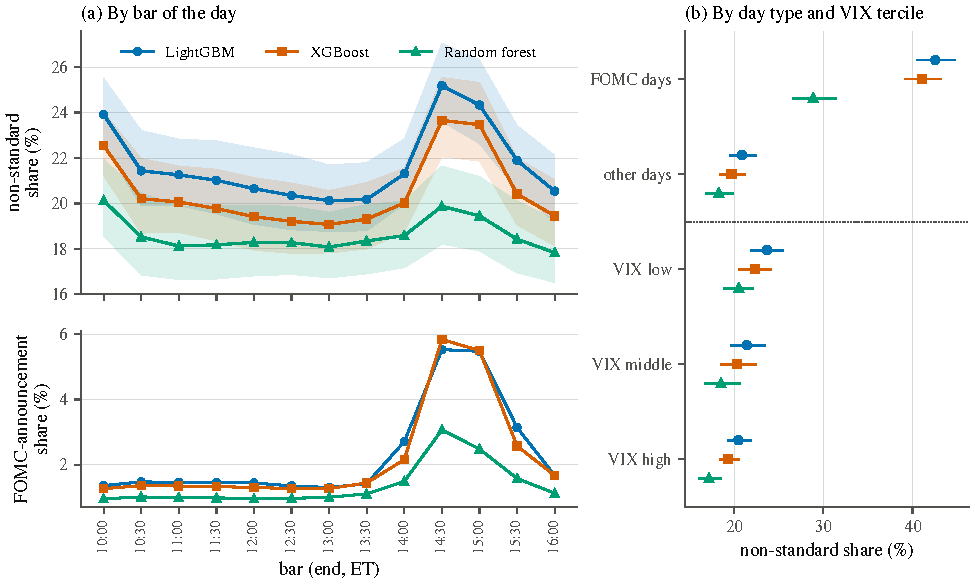
\includegraphics[width=\linewidth]{figures/fi_pooled/fip_cond.pdf}
\caption{When the tree ensembles use the non-standard series. Share of the non-standard series in the total mean absolute SHAP value on subsets of the \rhfipNRows{} bars, with \rhfipCiLevel\% block-bootstrap intervals over the origins. (a) By bar of the day (top; bands: intervals) and the FOMC-announcement category's share (bottom). (b) On the \rhfipFomcDays{} scheduled FOMC statement days and on all other days, and by the tercile of the VIX close before the origin (cut points \rhfipVixLo{} and \rhfipVixHi; every bar of an origin's block takes that origin's tercile).}
\label{fig:rh_fip_cond}
\end{figure}


% ---------------------------------------------------------------------------------------------------------------------
% 2026-10-26 (integration, JFEc): moved from 08_feature_importance.tex, "Shape of the response" and "Interactions".
\subsection{Variable importance: response shapes and interactions}
\label{app:rh_fi_shapes}
\begin{itemize}
\item \textbf{Shape of the response} (Table~\ref{tab:rh_fip_nonstd}, Figure~\ref{fig:rh_fip_shapes}). For each
  non-standard series with a share of at least \rhfipShapeMin\% in a tree (\rhfipLgbmNShape, \rhfipXgbNShape{} and
  \rhfipRfNShape{} series), the mean SHAP value by decile of its dominant predictor is classified by a rule fixed in
  advance: monotone \rhfipLgbmNMono, \rhfipXgbNMono{} and \rhfipRfNMono; irregular \rhfipLgbmNIrr, \rhfipXgbNIrr{} and
  \rhfipRfNIrr; a step \rhfipLgbmNStep, \rhfipXgbNStep{} and \rhfipRfNStep; flat \rhfipLgbmNFlat, \rhfipXgbNFlat{} and
  \rhfipRfNFlat; none U-shaped, inverted-U or a threshold. Most responses are one-sided (asymmetric: \rhfipLgbmNAsym,
  \rhfipXgbNAsym{} and \rhfipRfNAsym).
  \begin{itemize}
  \item The market's cross-sectional absolute returns and the spreads rise monotonically and are asymmetric toward
    the top tail: \rhfipAbsVw{} moves the forecast from \rhfipAbsVwLgbmLo\% of the mean forecast in its bottom
    decile to \rhfipAbsVwLgbmHi\% in its top decile (LightGBM; XGBoost \rhfipAbsVwXgbHi\%, forest \rhfipAbsVwRfHi\%).
  \item \rhfipOfi{} falls monotonically: a larger order-flow imbalance lowers the forecast, from \rhfipOfiLgbmLo\% to
    \rhfipOfiLgbmHi\% (LightGBM).
  \item \rhfipFomcUntil{} (dominant predictor: its average over $k = \rhfipUntilHorizon$ samples) is labeled irregular
    by the rule; read from the figure (post hoc), it is flat through the lower deciles and jumps in the top decile,
    the approach of a statement, to \rhfipUntilLgbmHi, \rhfipUntilXgbHi{} and \rhfipUntilRfHi\% of the mean forecast.
  \end{itemize}
\item \textbf{Interactions} (Table~\ref{tab:rh_fip_inter}; boosted trees, \rhfipInterRows{} bars, descriptive).
  Interactions carry \rhfipLgbmInterVar{} and \rhfipXgbInterVar\% of the attribution at the group level
  (\rhfipLgbmInterCol{} and \rhfipXgbInterCol\% at the predictor level). They carry \rhfipLgbmInterNs{} and
  \rhfipXgbInterNs\% of a non-standard series' attribution against \rhfipLgbmInterStd{} and \rhfipXgbInterStd\% for
  the standard groups; more than half of that gap comes from the HAR components, which act mostly on their own
  (\rhfipLgbmInterHar\% through interactions in LightGBM), and the calendar dummies: the standard exogenous series
  alone reach \rhfipLgbmInterStdEx{} and \rhfipXgbInterStdEx\% (descriptive). The largest pairs with a non-standard
  series pair it with the HAR components, \rhfipPairOneA{} $\times$ \rhfipPairOneB{} (\rhfipLgbmPairOne{} and
  \rhfipXgbPairOne\% of the pair total) and \rhfipPairTwoA{} $\times$ \rhfipPairTwoB{} (\rhfipLgbmPairTwo{} and
  \rhfipXgbPairTwo\%), and the HAR components are in \rhfipLgbmPairsHar{} and \rhfipXgbPairsHar{} of the ten largest.
  The weakest series act mostly through interactions: \rhfipLgbmInterWeakMin--\rhfipLgbmInterWeakMax\% of the
  attribution of the StockTwits series, VVIX, VIX3M and \rhfipFomcDay{} (LightGBM).
\end{itemize}
% Response shapes of the leading non-standard series (mean SHAP by decile of the dominant predictor)
% AUTO-GENERATED by writeup/make_rehaul_fi_pooled.py -- do not edit; re-run the script.
\providecommand{\ser}[2]{#2}\providecommand{\serx}[3]{#3}
\ifdefined\rhfipNOrigins\else% AUTO-GENERATED by writeup/make_rehaul_fi_pooled.py -- do not edit; re-run the script.
\providecommand{\ser}[2]{#2}\providecommand{\serx}[3]{#3}
% \rhfip... macros for writeup/rehaul/08_feature_importance.tex (results/tree_shap_w3000_2014start_fomcfix_2026-10-26, the
% FOMC-patched design, its linear reference inputs/fiw_gamma_fomcfix.npz; the window study's ...W... macros:
% results/fi_by_window_2014start_2026-10-22, pre-patch; the final pooled runs, W = 3,000 trading days).
\providecommand{\rhfipNOrigins}{}\renewcommand{\rhfipNOrigins}{126}  % monthly origins (re-estimations explained)
\providecommand{\rhfipNRows}{}\renewcommand{\rhfipNRows}{33{,}970}  % bars explained, every bar of the evaluation span
\providecommand{\rhfipOriginEvery}{}\renewcommand{\rhfipOriginEvery}{21}  % trading days between origins
\providecommand{\rhfipLastBlock}{}\renewcommand{\rhfipLastBlock}{18}  % trading days of the last origin's block
\providecommand{\rhfipFirstOrigin}{}\renewcommand{\rhfipFirstOrigin}{2~January~2014}  % first origin (10:00 bar)
\providecommand{\rhfipLastOrigin}{}\renewcommand{\rhfipLastOrigin}{5~April~2024}  % last origin
\providecommand{\rhfipLastDay}{}\renewcommand{\rhfipLastDay}{30~April~2024}  % day of the last bar explained
\providecommand{\rhfipWindowDays}{}\renewcommand{\rhfipWindowDays}{3{,}000}  % rolling window, trading days
\providecommand{\rhfipWindowBars}{}\renewcommand{\rhfipWindowBars}{39{,}000}  % rolling window, bars
\providecommand{\rhfipNCols}{}\renewcommand{\rhfipNCols}{564}  % predictors of the full set
\providecommand{\rhfipNGroups}{}\renewcommand{\rhfipNGroups}{48}  % predictor groups: 46 exogenous series + HAR components + calendar dummies
\providecommand{\rhfipNExog}{}\renewcommand{\rhfipNExog}{46}  % exogenous series
\providecommand{\rhfipNPerSeries}{}\renewcommand{\rhfipNPerSeries}{12}  % predictors per exogenous series: value and availability averages at six horizons
\providecommand{\rhfipNStd}{}\renewcommand{\rhfipNStd}{12}  % standard groups
\providecommand{\rhfipNNonStd}{}\renewcommand{\rhfipNNonStd}{36}  % non-standard series
\providecommand{\rhfipNStdExog}{}\renewcommand{\rhfipNStdExog}{10}  % standard exogenous series
\providecommand{\rhfipTuneLast}{}\renewcommand{\rhfipTuneLast}{31~December~2013}  % last day of the last tuning fold (fold 3)
\providecommand{\rhfipRidgePen}{}\renewcommand{\rhfipRidgePen}{\ensuremath{10^{3}}}
\providecommand{\rhfipLassoPen}{}\renewcommand{\rhfipLassoPen}{\ensuremath{10^{-4}}}
\providecommand{\rhfipEnetPen}{}\renewcommand{\rhfipEnetPen}{\ensuremath{10^{-3}}}
\providecommand{\rhfipHarPf}{}\renewcommand{\rhfipHarPf}{0.01}  % penalty factor, HAR block
\providecommand{\rhfipBootBlock}{}\renewcommand{\rhfipBootBlock}{12}  % bootstrap block, origins
\providecommand{\rhfipBootB}{}\renewcommand{\rhfipBootB}{2{,}000}
\providecommand{\rhfipCiLevel}{}\renewcommand{\rhfipCiLevel}{95}  % percentile intervals of both rules (RULE_shap.txt, RULE_fiw.txt)
\providecommand{\rhfipShapeMin}{}\renewcommand{\rhfipShapeMin}{0.5}  % M3 selection: share of at least this many percent
\providecommand{\rhfipTopN}{}\renewcommand{\rhfipTopN}{10}  % length of the top lists compared (m2_rank.csv top10_overlap)
\providecommand{\rhfipSlopeUnit}{}\renewcommand{\rhfipSlopeUnit}{1{,}000}  % trading days per unit of the window slope
\providecommand{\rhfipNMom}{}\renewcommand{\rhfipNMom}{seven}  % the futures' realized moments (standard)
\providecommand{\rhfipLgbmGateEq}{}\renewcommand{\rhfipLgbmGateEq}{126}  % origins bit-equal to the merged every-bar walk
\providecommand{\rhfipXgbGateEq}{}\renewcommand{\rhfipXgbGateEq}{126}  % origins bit-equal to the merged every-bar walk
\providecommand{\rhfipRfGateEq}{}\renewcommand{\rhfipRfGateEq}{126}  % origins bit-equal to the merged every-bar walk
\providecommand{\rhfipRfGateAtShap}{}\renewcommand{\rhfipRfGateAtShap}{126}  % forest origins the walk had written when the SHAP gate ran
\providecommand{\rhfipXgbAddMax}{}\renewcommand{\rhfipXgbAddMax}{\ensuremath{3.7\times 10^{-6}}}  % XGBoost additivity, float32
\providecommand{\rhfipXgbAddTol}{}\renewcommand{\rhfipXgbAddTol}{\ensuremath{10^{-5}}}
\providecommand{\rhfipAddMaxDouble}{}\renewcommand{\rhfipAddMaxDouble}{\ensuremath{5.1\times 10^{-14}}}
\providecommand{\rhfipLinGateMax}{}\renewcommand{\rhfipLinGateMax}{\ensuremath{4.4\times 10^{-16}}}  % linear replay vs walk forecasts, W = 3,000
\providecommand{\rhfipInterRows}{}\renewcommand{\rhfipInterRows}{1{,}008}  % M5 rows
\providecommand{\rhfipInterPerOrigin}{}\renewcommand{\rhfipInterPerOrigin}{8}  % M5 rows per origin
\providecommand{\rhfipFomcRows}{}\renewcommand{\rhfipFomcRows}{1{,}014}
\providecommand{\rhfipFomcDaysShap}{}\renewcommand{\rhfipFomcDaysShap}{78}  % FOMC statement days in the SHAP subset (M4; releases.parquet only)
\providecommand{\rhfipFomcDays}{}\renewcommand{\rhfipFomcDays}{81}  % scheduled FOMC statement days in the span (loader calendar)
\providecommand{\rhfipFomcDaysMissing}{}\renewcommand{\rhfipFomcDaysMissing}{3}  % statement days the SHAP subset leaves out (counted with the other days; the patched rerun's reducer keeps releases.parquet's days)
\providecommand{\rhfipNHolSessions}{}\renewcommand{\rhfipNHolSessions}{64}  % NYSE-holiday futures sessions among the explained bars (not scored in Table 1)
\providecommand{\rhfipNHolBars}{}\renewcommand{\rhfipNHolBars}{443}  % their regular-hours bars
\providecommand{\rhfipVixLo}{}\renewcommand{\rhfipVixLo}{13.96}
\providecommand{\rhfipVixHi}{}\renewcommand{\rhfipVixHi}{19.02}
\providecommand{\rhfipLgbmHar}{}\renewcommand{\rhfipLgbmHar}{51.7}
\providecommand{\rhfipLgbmHarLo}{}\renewcommand{\rhfipLgbmHarLo}{49.5}
\providecommand{\rhfipLgbmHarHi}{}\renewcommand{\rhfipLgbmHarHi}{53.7}
\providecommand{\rhfipLgbmMom}{}\renewcommand{\rhfipLgbmMom}{22.3}
\providecommand{\rhfipLgbmNs}{}\renewcommand{\rhfipLgbmNs}{21.8}
\providecommand{\rhfipLgbmNsLo}{}\renewcommand{\rhfipLgbmNsLo}{20.4}
\providecommand{\rhfipLgbmNsHi}{}\renewcommand{\rhfipLgbmNsHi}{23.4}
\providecommand{\rhfipLgbmNsEx}{}\renewcommand{\rhfipLgbmNsEx}{45.9}
\providecommand{\rhfipLgbmNsExLo}{}\renewcommand{\rhfipLgbmNsExLo}{44.2}
\providecommand{\rhfipLgbmNsExHi}{}\renewcommand{\rhfipLgbmNsExHi}{47.7}
\providecommand{\rhfipXgbHar}{}\renewcommand{\rhfipXgbHar}{52.0}
\providecommand{\rhfipXgbHarLo}{}\renewcommand{\rhfipXgbHarLo}{50.0}
\providecommand{\rhfipXgbHarHi}{}\renewcommand{\rhfipXgbHarHi}{53.8}
\providecommand{\rhfipXgbMom}{}\renewcommand{\rhfipXgbMom}{23.6}
\providecommand{\rhfipXgbNs}{}\renewcommand{\rhfipXgbNs}{20.6}
\providecommand{\rhfipXgbNsLo}{}\renewcommand{\rhfipXgbNsLo}{19.2}
\providecommand{\rhfipXgbNsHi}{}\renewcommand{\rhfipXgbNsHi}{22.2}
\providecommand{\rhfipXgbNsEx}{}\renewcommand{\rhfipXgbNsEx}{43.6}
\providecommand{\rhfipXgbNsExLo}{}\renewcommand{\rhfipXgbNsExLo}{41.8}
\providecommand{\rhfipXgbNsExHi}{}\renewcommand{\rhfipXgbNsExHi}{45.7}
\providecommand{\rhfipRfHar}{}\renewcommand{\rhfipRfHar}{57.6}
\providecommand{\rhfipRfHarLo}{}\renewcommand{\rhfipRfHarLo}{55.4}
\providecommand{\rhfipRfHarHi}{}\renewcommand{\rhfipRfHarHi}{59.6}
\providecommand{\rhfipRfMom}{}\renewcommand{\rhfipRfMom}{20.7}
\providecommand{\rhfipRfNs}{}\renewcommand{\rhfipRfNs}{18.6}
\providecommand{\rhfipRfNsLo}{}\renewcommand{\rhfipRfNsLo}{17.2}
\providecommand{\rhfipRfNsHi}{}\renewcommand{\rhfipRfNsHi}{20.3}
\providecommand{\rhfipRfNsEx}{}\renewcommand{\rhfipRfNsEx}{44.2}
\providecommand{\rhfipRfNsExLo}{}\renewcommand{\rhfipRfNsExLo}{42.1}
\providecommand{\rhfipRfNsExHi}{}\renewcommand{\rhfipRfNsExHi}{46.5}
\providecommand{\rhfipRidgeNsEx}{}\renewcommand{\rhfipRidgeNsEx}{68.8}
\providecommand{\rhfipRidgeNs}{}\renewcommand{\rhfipRidgeNs}{55.6}
\providecommand{\rhfipRidgeHar}{}\renewcommand{\rhfipRidgeHar}{17.5}
\providecommand{\rhfipLassoNsEx}{}\renewcommand{\rhfipLassoNsEx}{82.5}
\providecommand{\rhfipLassoNs}{}\renewcommand{\rhfipLassoNs}{76.5}
\providecommand{\rhfipLassoHar}{}\renewcommand{\rhfipLassoHar}{6.7}
\providecommand{\rhfipEnetNsEx}{}\renewcommand{\rhfipEnetNsEx}{60.0}
\providecommand{\rhfipEnetNs}{}\renewcommand{\rhfipEnetNs}{42.9}
\providecommand{\rhfipEnetHar}{}\renewcommand{\rhfipEnetHar}{26.4}
\providecommand{\rhfipHarMin}{}\renewcommand{\rhfipHarMin}{51.7}
\providecommand{\rhfipHarMax}{}\renewcommand{\rhfipHarMax}{57.6}
\providecommand{\rhfipMomMin}{}\renewcommand{\rhfipMomMin}{20.7}
\providecommand{\rhfipMomMax}{}\renewcommand{\rhfipMomMax}{23.6}
\providecommand{\rhfipNsExMin}{}\renewcommand{\rhfipNsExMin}{43.6}
\providecommand{\rhfipNsExMax}{}\renewcommand{\rhfipNsExMax}{45.9}
\providecommand{\rhfipSentMin}{}\renewcommand{\rhfipSentMin}{0.6}
\providecommand{\rhfipSentMax}{}\renewcommand{\rhfipSentMax}{0.8}
\providecommand{\rhfipVdMin}{}\renewcommand{\rhfipVdMin}{0.2}
\providecommand{\rhfipVdMax}{}\renewcommand{\rhfipVdMax}{0.3}
\providecommand{\rhfipFomcBucketMin}{}\renewcommand{\rhfipFomcBucketMin}{1.4}
\providecommand{\rhfipFomcBucketMax}{}\renewcommand{\rhfipFomcBucketMax}{2.3}
\providecommand{\rhfipVvixMin}{}\renewcommand{\rhfipVvixMin}{0.2}
\providecommand{\rhfipVvixMax}{}\renewcommand{\rhfipVvixMax}{0.3}
\providecommand{\rhfipVixThreeMMin}{}\renewcommand{\rhfipVixThreeMMin}{0.3}
\providecommand{\rhfipVixThreeMMax}{}\renewcommand{\rhfipVixThreeMMax}{0.7}
\providecommand{\rhfipFomcDayMin}{}\renewcommand{\rhfipFomcDayMin}{0.1}
\providecommand{\rhfipFomcDayMax}{}\renewcommand{\rhfipFomcDayMax}{0.1}
\providecommand{\rhfipNsOne}{}\renewcommand{\rhfipNsOne}{\ensuremath{\ser{sumabsret_vwstock}{\mathrm{RAV}^{\mathrm{VW}}}}}
\providecommand{\rhfipNsOneMin}{}\renewcommand{\rhfipNsOneMin}{2.4}
\providecommand{\rhfipNsOneMax}{}\renewcommand{\rhfipNsOneMax}{3.9}
\providecommand{\rhfipNsOneLgbm}{}\renewcommand{\rhfipNsOneLgbm}{3.5}
\providecommand{\rhfipNsOneXgb}{}\renewcommand{\rhfipNsOneXgb}{3.9}
\providecommand{\rhfipNsOneRf}{}\renewcommand{\rhfipNsOneRf}{2.4}
\providecommand{\rhfipNsTwo}{}\renewcommand{\rhfipNsTwo}{\ensuremath{\ser{sumabsret_ewstock}{\mathrm{RAV}^{\mathrm{EW}}}}}
\providecommand{\rhfipNsTwoMin}{}\renewcommand{\rhfipNsTwoMin}{1.9}
\providecommand{\rhfipNsTwoMax}{}\renewcommand{\rhfipNsTwoMax}{3.9}
\providecommand{\rhfipNsTwoLgbm}{}\renewcommand{\rhfipNsTwoLgbm}{3.9}
\providecommand{\rhfipNsTwoXgb}{}\renewcommand{\rhfipNsTwoXgb}{3.8}
\providecommand{\rhfipNsTwoRf}{}\renewcommand{\rhfipNsTwoRf}{1.9}
\providecommand{\rhfipNsThree}{}\renewcommand{\rhfipNsThree}{\ensuremath{\ser{fomc_until_inv}{\mathrm{FOMC}^{\mathrm{next}}}}}
\providecommand{\rhfipNsThreeMin}{}\renewcommand{\rhfipNsThreeMin}{1.1}
\providecommand{\rhfipNsThreeMax}{}\renewcommand{\rhfipNsThreeMax}{2.0}
\providecommand{\rhfipNsThreeLgbm}{}\renewcommand{\rhfipNsThreeLgbm}{2.0}
\providecommand{\rhfipNsThreeXgb}{}\renewcommand{\rhfipNsThreeXgb}{2.0}
\providecommand{\rhfipNsThreeRf}{}\renewcommand{\rhfipNsThreeRf}{1.1}
\providecommand{\rhfipNsFour}{}\renewcommand{\rhfipNsFour}{\ensuremath{\ser{ofi_vwstock}{\mathrm{OFI}^{\mathrm{VW}}}}}
\providecommand{\rhfipNsFourMin}{}\renewcommand{\rhfipNsFourMin}{1.4}
\providecommand{\rhfipNsFourMax}{}\renewcommand{\rhfipNsFourMax}{1.8}
\providecommand{\rhfipNsFourLgbm}{}\renewcommand{\rhfipNsFourLgbm}{1.8}
\providecommand{\rhfipNsFourXgb}{}\renewcommand{\rhfipNsFourXgb}{1.7}
\providecommand{\rhfipNsFourRf}{}\renewcommand{\rhfipNsFourRf}{1.4}
\providecommand{\rhfipNsFive}{}\renewcommand{\rhfipNsFive}{\ensuremath{\ser{effspread_vwstock}{\mathrm{EffSpread}^{\mathrm{VW}}}}}
\providecommand{\rhfipNsFiveMin}{}\renewcommand{\rhfipNsFiveMin}{1.2}
\providecommand{\rhfipNsFiveMax}{}\renewcommand{\rhfipNsFiveMax}{1.3}
\providecommand{\rhfipNsFiveLgbm}{}\renewcommand{\rhfipNsFiveLgbm}{1.2}
\providecommand{\rhfipNsFiveXgb}{}\renewcommand{\rhfipNsFiveXgb}{1.2}
\providecommand{\rhfipNsFiveRf}{}\renewcommand{\rhfipNsFiveRf}{1.3}
\providecommand{\rhfipTreeTopOne}{}\renewcommand{\rhfipTreeTopOne}{\ensuremath{\ser{sumabsret}{\mathrm{RAV}}}}
\providecommand{\rhfipTreeTopTwo}{}\renewcommand{\rhfipTreeTopTwo}{\ensuremath{\ser{sumret}{r}}}
\providecommand{\rhfipLgbmTopOneEx}{}\renewcommand{\rhfipLgbmTopOneEx}{20.3}
\providecommand{\rhfipXgbTopOneEx}{}\renewcommand{\rhfipXgbTopOneEx}{24.7}
\providecommand{\rhfipRfTopOneEx}{}\renewcommand{\rhfipRfTopOneEx}{29.2}
\providecommand{\rhfipRidgeTopOne}{}\renewcommand{\rhfipRidgeTopOne}{\ensuremath{\ser{fomc_until_inv}{\mathrm{FOMC}^{\mathrm{next}}}}}
\providecommand{\rhfipRidgeTopOneEx}{}\renewcommand{\rhfipRidgeTopOneEx}{9.0}
\providecommand{\rhfipLgbmNUsedAll}{}\renewcommand{\rhfipLgbmNUsedAll}{42}  % exogenous series split on at every origin
\providecommand{\rhfipLgbmUsedMin}{}\renewcommand{\rhfipLgbmUsedMin}{58}
\providecommand{\rhfipXgbNUsedAll}{}\renewcommand{\rhfipXgbNUsedAll}{43}  % exogenous series split on at every origin
\providecommand{\rhfipXgbUsedMin}{}\renewcommand{\rhfipXgbUsedMin}{72}
\providecommand{\rhfipRfNUsedAll}{}\renewcommand{\rhfipRfNUsedAll}{46}  % exogenous series split on at every origin
\providecommand{\rhfipRfUsedMin}{}\renewcommand{\rhfipRfUsedMin}{126}
\providecommand{\rhfipLgbmDRidge}{}\renewcommand{\rhfipLgbmDRidge}{\ensuremath{-}22.9}
\providecommand{\rhfipLgbmDRidgeLo}{}\renewcommand{\rhfipLgbmDRidgeLo}{\ensuremath{-}24.8}
\providecommand{\rhfipLgbmDRidgeHi}{}\renewcommand{\rhfipLgbmDRidgeHi}{\ensuremath{-}21.1}
\providecommand{\rhfipLgbmDLasso}{}\renewcommand{\rhfipLgbmDLasso}{\ensuremath{-}36.6}
\providecommand{\rhfipLgbmDLassoLo}{}\renewcommand{\rhfipLgbmDLassoLo}{\ensuremath{-}39.1}
\providecommand{\rhfipLgbmDLassoHi}{}\renewcommand{\rhfipLgbmDLassoHi}{\ensuremath{-}34.4}
\providecommand{\rhfipLgbmDEnet}{}\renewcommand{\rhfipLgbmDEnet}{\ensuremath{-}14.1}
\providecommand{\rhfipLgbmDEnetLo}{}\renewcommand{\rhfipLgbmDEnetLo}{\ensuremath{-}15.7}
\providecommand{\rhfipLgbmDEnetHi}{}\renewcommand{\rhfipLgbmDEnetHi}{\ensuremath{-}12.7}
\providecommand{\rhfipXgbDRidge}{}\renewcommand{\rhfipXgbDRidge}{\ensuremath{-}25.1}
\providecommand{\rhfipXgbDRidgeLo}{}\renewcommand{\rhfipXgbDRidgeLo}{\ensuremath{-}27.0}
\providecommand{\rhfipXgbDRidgeHi}{}\renewcommand{\rhfipXgbDRidgeHi}{\ensuremath{-}23.3}
\providecommand{\rhfipXgbDLasso}{}\renewcommand{\rhfipXgbDLasso}{\ensuremath{-}38.9}
\providecommand{\rhfipXgbDLassoLo}{}\renewcommand{\rhfipXgbDLassoLo}{\ensuremath{-}41.4}
\providecommand{\rhfipXgbDLassoHi}{}\renewcommand{\rhfipXgbDLassoHi}{\ensuremath{-}36.6}
\providecommand{\rhfipXgbDEnet}{}\renewcommand{\rhfipXgbDEnet}{\ensuremath{-}16.3}
\providecommand{\rhfipXgbDEnetLo}{}\renewcommand{\rhfipXgbDEnetLo}{\ensuremath{-}17.8}
\providecommand{\rhfipXgbDEnetHi}{}\renewcommand{\rhfipXgbDEnetHi}{\ensuremath{-}14.9}
\providecommand{\rhfipRfDRidge}{}\renewcommand{\rhfipRfDRidge}{\ensuremath{-}24.5}
\providecommand{\rhfipRfDRidgeLo}{}\renewcommand{\rhfipRfDRidgeLo}{\ensuremath{-}26.3}
\providecommand{\rhfipRfDRidgeHi}{}\renewcommand{\rhfipRfDRidgeHi}{\ensuremath{-}22.9}
\providecommand{\rhfipRfDLasso}{}\renewcommand{\rhfipRfDLasso}{\ensuremath{-}38.3}
\providecommand{\rhfipRfDLassoLo}{}\renewcommand{\rhfipRfDLassoLo}{\ensuremath{-}40.5}
\providecommand{\rhfipRfDLassoHi}{}\renewcommand{\rhfipRfDLassoHi}{\ensuremath{-}36.3}
\providecommand{\rhfipRfDEnet}{}\renewcommand{\rhfipRfDEnet}{\ensuremath{-}15.7}
\providecommand{\rhfipRfDEnetLo}{}\renewcommand{\rhfipRfDEnetLo}{\ensuremath{-}17.0}
\providecommand{\rhfipRfDEnetHi}{}\renewcommand{\rhfipRfDEnetHi}{\ensuremath{-}14.4}
\providecommand{\rhfipNDLess}{}\renewcommand{\rhfipNDLess}{27}  % tree-minus-linear D with the 95% interval below 0
\providecommand{\rhfipNDAll}{}\renewcommand{\rhfipNDAll}{27}  % D comparisons: 3 trees x 3 linear models x 3 denominators
\providecommand{\rhfipLgbmSpRidge}{}\renewcommand{\rhfipLgbmSpRidge}{0.57}
\providecommand{\rhfipLgbmTopRidge}{}\renewcommand{\rhfipLgbmTopRidge}{6}
\providecommand{\rhfipLgbmSpLasso}{}\renewcommand{\rhfipLgbmSpLasso}{0.49}
\providecommand{\rhfipLgbmTopLasso}{}\renewcommand{\rhfipLgbmTopLasso}{5}
\providecommand{\rhfipLgbmSpEnet}{}\renewcommand{\rhfipLgbmSpEnet}{0.66}
\providecommand{\rhfipLgbmTopEnet}{}\renewcommand{\rhfipLgbmTopEnet}{6}
\providecommand{\rhfipXgbSpRidge}{}\renewcommand{\rhfipXgbSpRidge}{0.55}
\providecommand{\rhfipXgbTopRidge}{}\renewcommand{\rhfipXgbTopRidge}{6}
\providecommand{\rhfipXgbSpLasso}{}\renewcommand{\rhfipXgbSpLasso}{0.47}
\providecommand{\rhfipXgbTopLasso}{}\renewcommand{\rhfipXgbTopLasso}{5}
\providecommand{\rhfipXgbSpEnet}{}\renewcommand{\rhfipXgbSpEnet}{0.63}
\providecommand{\rhfipXgbTopEnet}{}\renewcommand{\rhfipXgbTopEnet}{6}
\providecommand{\rhfipRfSpRidge}{}\renewcommand{\rhfipRfSpRidge}{0.53}
\providecommand{\rhfipRfTopRidge}{}\renewcommand{\rhfipRfTopRidge}{5}
\providecommand{\rhfipRfSpLasso}{}\renewcommand{\rhfipRfSpLasso}{0.43}
\providecommand{\rhfipRfTopLasso}{}\renewcommand{\rhfipRfTopLasso}{4}
\providecommand{\rhfipRfSpEnet}{}\renewcommand{\rhfipRfSpEnet}{0.60}
\providecommand{\rhfipRfTopEnet}{}\renewcommand{\rhfipRfTopEnet}{5}
\providecommand{\rhfipSpLgbmXgb}{}\renewcommand{\rhfipSpLgbmXgb}{0.99}
\providecommand{\rhfipSpLgbmRf}{}\renewcommand{\rhfipSpLgbmRf}{0.90}
\providecommand{\rhfipSpXgbRf}{}\renewcommand{\rhfipSpXgbRf}{0.89}
\providecommand{\rhfipRidgeRankFomcUntil}{}\renewcommand{\rhfipRidgeRankFomcUntil}{1}
\providecommand{\rhfipTreeRankFomcUntilMin}{}\renewcommand{\rhfipTreeRankFomcUntilMin}{6}
\providecommand{\rhfipTreeRankFomcUntilMax}{}\renewcommand{\rhfipTreeRankFomcUntilMax}{10}
\providecommand{\rhfipRidgeRankFomcDay}{}\renewcommand{\rhfipRidgeRankFomcDay}{9}
\providecommand{\rhfipTreeRankFomcDayMin}{}\renewcommand{\rhfipTreeRankFomcDayMin}{39}
\providecommand{\rhfipTreeRankFomcDayMax}{}\renewcommand{\rhfipTreeRankFomcDayMax}{43}
\providecommand{\rhfipFomcUntil}{}\renewcommand{\rhfipFomcUntil}{\ensuremath{\ser{fomc_until_inv}{\mathrm{FOMC}^{\mathrm{next}}}}}
\providecommand{\rhfipFomcDay}{}\renewcommand{\rhfipFomcDay}{\ensuremath{\ser{fomc_day}{\mathrm{FOMC}^{\mathrm{day}}}}}
\providecommand{\rhfipAbsVw}{}\renewcommand{\rhfipAbsVw}{\ensuremath{\ser{sumabsret_vwstock}{\mathrm{RAV}^{\mathrm{VW}}}}}
\providecommand{\rhfipOfi}{}\renewcommand{\rhfipOfi}{\ensuremath{\ser{ofi_vwstock}{\mathrm{OFI}^{\mathrm{VW}}}}}
\providecommand{\rhfipLgbmNeff}{}\renewcommand{\rhfipLgbmNeff}{11.0}
\providecommand{\rhfipLgbmNHalf}{}\renewcommand{\rhfipLgbmNHalf}{4}
\providecommand{\rhfipLgbmNEighty}{}\renewcommand{\rhfipLgbmNEighty}{13}
\providecommand{\rhfipXgbNeff}{}\renewcommand{\rhfipXgbNeff}{9.1}
\providecommand{\rhfipXgbNHalf}{}\renewcommand{\rhfipXgbNHalf}{4}
\providecommand{\rhfipXgbNEighty}{}\renewcommand{\rhfipXgbNEighty}{11}
\providecommand{\rhfipRfNeff}{}\renewcommand{\rhfipRfNeff}{8.9}
\providecommand{\rhfipRfNHalf}{}\renewcommand{\rhfipRfNHalf}{4}
\providecommand{\rhfipRfNEighty}{}\renewcommand{\rhfipRfNEighty}{16}
\providecommand{\rhfipRidgeNeff}{}\renewcommand{\rhfipRidgeNeff}{28.5}
\providecommand{\rhfipRidgeNHalf}{}\renewcommand{\rhfipRidgeNHalf}{11}
\providecommand{\rhfipRidgeNEighty}{}\renewcommand{\rhfipRidgeNEighty}{26}
\providecommand{\rhfipLassoNeff}{}\renewcommand{\rhfipLassoNeff}{5.1}
\providecommand{\rhfipLassoNHalf}{}\renewcommand{\rhfipLassoNHalf}{2}
\providecommand{\rhfipLassoNEighty}{}\renewcommand{\rhfipLassoNEighty}{11}
\providecommand{\rhfipEnetNeff}{}\renewcommand{\rhfipEnetNeff}{16.2}
\providecommand{\rhfipEnetNHalf}{}\renewcommand{\rhfipEnetNHalf}{6}
\providecommand{\rhfipEnetNEighty}{}\renewcommand{\rhfipEnetNEighty}{15}
\providecommand{\rhfipYearFirst}{}\renewcommand{\rhfipYearFirst}{2014}
\providecommand{\rhfipYearLast}{}\renewcommand{\rhfipYearLast}{2024}
\providecommand{\rhfipLgbmNsYearMin}{}\renewcommand{\rhfipLgbmNsYearMin}{18.1}
\providecommand{\rhfipLgbmNsYearMinYr}{}\renewcommand{\rhfipLgbmNsYearMinYr}{2021}
\providecommand{\rhfipLgbmNsYearMax}{}\renewcommand{\rhfipLgbmNsYearMax}{25.6}
\providecommand{\rhfipLgbmNsYearMaxYr}{}\renewcommand{\rhfipLgbmNsYearMaxYr}{2015}
\providecommand{\rhfipLgbmHarYearMax}{}\renewcommand{\rhfipLgbmHarYearMax}{57.4}
\providecommand{\rhfipLgbmHarYearMaxYr}{}\renewcommand{\rhfipLgbmHarYearMaxYr}{2021}
\providecommand{\rhfipLgbmHarYearMin}{}\renewcommand{\rhfipLgbmHarYearMin}{44.6}
\providecommand{\rhfipLgbmHarYearMinYr}{}\renewcommand{\rhfipLgbmHarYearMinYr}{2017}
\providecommand{\rhfipXgbNsYearMin}{}\renewcommand{\rhfipXgbNsYearMin}{17.2}
\providecommand{\rhfipXgbNsYearMinYr}{}\renewcommand{\rhfipXgbNsYearMinYr}{2021}
\providecommand{\rhfipXgbNsYearMax}{}\renewcommand{\rhfipXgbNsYearMax}{24.3}
\providecommand{\rhfipXgbNsYearMaxYr}{}\renewcommand{\rhfipXgbNsYearMaxYr}{2015}
\providecommand{\rhfipXgbHarYearMax}{}\renewcommand{\rhfipXgbHarYearMax}{57.0}
\providecommand{\rhfipXgbHarYearMaxYr}{}\renewcommand{\rhfipXgbHarYearMaxYr}{2021}
\providecommand{\rhfipXgbHarYearMin}{}\renewcommand{\rhfipXgbHarYearMin}{45.8}
\providecommand{\rhfipXgbHarYearMinYr}{}\renewcommand{\rhfipXgbHarYearMinYr}{2017}
\providecommand{\rhfipRfNsYearMin}{}\renewcommand{\rhfipRfNsYearMin}{15.2}
\providecommand{\rhfipRfNsYearMinYr}{}\renewcommand{\rhfipRfNsYearMinYr}{2021}
\providecommand{\rhfipRfNsYearMax}{}\renewcommand{\rhfipRfNsYearMax}{22.9}
\providecommand{\rhfipRfNsYearMaxYr}{}\renewcommand{\rhfipRfNsYearMaxYr}{2015}
\providecommand{\rhfipRfHarYearMax}{}\renewcommand{\rhfipRfHarYearMax}{62.3}
\providecommand{\rhfipRfHarYearMaxYr}{}\renewcommand{\rhfipRfHarYearMaxYr}{2019}
\providecommand{\rhfipRfHarYearMin}{}\renewcommand{\rhfipRfHarYearMin}{50.4}
\providecommand{\rhfipRfHarYearMinYr}{}\renewcommand{\rhfipRfHarYearMinYr}{2017}
\providecommand{\rhfipNsYearMinYr}{}\renewcommand{\rhfipNsYearMinYr}{2021}  % the year of every tree's lowest non-standard share
\providecommand{\rhfipDipFirst}{}\renewcommand{\rhfipDipFirst}{2018}  % first of the years in which every tree's non-standard share is below its pooled share
\providecommand{\rhfipDipLast}{}\renewcommand{\rhfipDipLast}{2022}
\providecommand{\rhfipRidgeNsExYearMin}{}\renewcommand{\rhfipRidgeNsExYearMin}{65.1}
\providecommand{\rhfipRidgeNsExYearMinYr}{}\renewcommand{\rhfipRidgeNsExYearMinYr}{2021}
\providecommand{\rhfipRidgeNsExYearMax}{}\renewcommand{\rhfipRidgeNsExYearMax}{72.4}
\providecommand{\rhfipRidgeNsExYearMaxYr}{}\renewcommand{\rhfipRidgeNsExYearMaxYr}{2017}
\providecommand{\rhfipLassoNsExYearMin}{}\renewcommand{\rhfipLassoNsExYearMin}{77.1}
\providecommand{\rhfipLassoNsExYearMinYr}{}\renewcommand{\rhfipLassoNsExYearMinYr}{2021}
\providecommand{\rhfipLassoNsExYearMax}{}\renewcommand{\rhfipLassoNsExYearMax}{87.1}
\providecommand{\rhfipLassoNsExYearMaxYr}{}\renewcommand{\rhfipLassoNsExYearMaxYr}{2017}
\providecommand{\rhfipEnetNsExYearMin}{}\renewcommand{\rhfipEnetNsExYearMin}{56.1}
\providecommand{\rhfipEnetNsExYearMinYr}{}\renewcommand{\rhfipEnetNsExYearMinYr}{2019}
\providecommand{\rhfipEnetNsExYearMax}{}\renewcommand{\rhfipEnetNsExYearMax}{65.2}
\providecommand{\rhfipEnetNsExYearMaxYr}{}\renewcommand{\rhfipEnetNsExYearMaxYr}{2014}
\providecommand{\rhfipLgbmNsExYearMin}{}\renewcommand{\rhfipLgbmNsExYearMin}{42.3}
\providecommand{\rhfipLgbmNsExYearMax}{}\renewcommand{\rhfipLgbmNsExYearMax}{50.1}
\providecommand{\rhfipXgbNsExYearMin}{}\renewcommand{\rhfipXgbNsExYearMin}{39.4}
\providecommand{\rhfipXgbNsExYearMax}{}\renewcommand{\rhfipXgbNsExYearMax}{48.9}
\providecommand{\rhfipRfNsExYearMin}{}\renewcommand{\rhfipRfNsExYearMin}{39.5}
\providecommand{\rhfipRfNsExYearMax}{}\renewcommand{\rhfipRfNsExYearMax}{50.9}
\providecommand{\rhfipLgbmNShape}{}\renewcommand{\rhfipLgbmNShape}{11}  % non-standard series at >= 0.5% (M3)
\providecommand{\rhfipLgbmNMono}{}\renewcommand{\rhfipLgbmNMono}{7}
\providecommand{\rhfipLgbmNIrr}{}\renewcommand{\rhfipLgbmNIrr}{3}
\providecommand{\rhfipLgbmNStep}{}\renewcommand{\rhfipLgbmNStep}{1}
\providecommand{\rhfipLgbmNFlat}{}\renewcommand{\rhfipLgbmNFlat}{0}
\providecommand{\rhfipLgbmNThresh}{}\renewcommand{\rhfipLgbmNThresh}{0}
\providecommand{\rhfipLgbmNU}{}\renewcommand{\rhfipLgbmNU}{0}
\providecommand{\rhfipLgbmNAsym}{}\renewcommand{\rhfipLgbmNAsym}{9}
\providecommand{\rhfipXgbNShape}{}\renewcommand{\rhfipXgbNShape}{10}  % non-standard series at >= 0.5% (M3)
\providecommand{\rhfipXgbNMono}{}\renewcommand{\rhfipXgbNMono}{5}
\providecommand{\rhfipXgbNIrr}{}\renewcommand{\rhfipXgbNIrr}{3}
\providecommand{\rhfipXgbNStep}{}\renewcommand{\rhfipXgbNStep}{0}
\providecommand{\rhfipXgbNFlat}{}\renewcommand{\rhfipXgbNFlat}{1}
\providecommand{\rhfipXgbNThresh}{}\renewcommand{\rhfipXgbNThresh}{1}
\providecommand{\rhfipXgbNU}{}\renewcommand{\rhfipXgbNU}{0}
\providecommand{\rhfipXgbNAsym}{}\renewcommand{\rhfipXgbNAsym}{8}
\providecommand{\rhfipRfNShape}{}\renewcommand{\rhfipRfNShape}{13}  % non-standard series at >= 0.5% (M3)
\providecommand{\rhfipRfNMono}{}\renewcommand{\rhfipRfNMono}{10}
\providecommand{\rhfipRfNIrr}{}\renewcommand{\rhfipRfNIrr}{3}
\providecommand{\rhfipRfNStep}{}\renewcommand{\rhfipRfNStep}{0}
\providecommand{\rhfipRfNFlat}{}\renewcommand{\rhfipRfNFlat}{0}
\providecommand{\rhfipRfNThresh}{}\renewcommand{\rhfipRfNThresh}{0}
\providecommand{\rhfipRfNU}{}\renewcommand{\rhfipRfNU}{0}
\providecommand{\rhfipRfNAsym}{}\renewcommand{\rhfipRfNAsym}{13}
\providecommand{\rhfipNUThreshAll}{}\renewcommand{\rhfipNUThreshAll}{1}  % U-shaped, inverted-U or threshold profiles in any tree
\providecommand{\rhfipAbsVwLgbmLo}{}\renewcommand{\rhfipAbsVwLgbmLo}{\ensuremath{-}1.4}
\providecommand{\rhfipAbsVwLgbmHi}{}\renewcommand{\rhfipAbsVwLgbmHi}{3.9}
\providecommand{\rhfipAbsVwXgbLo}{}\renewcommand{\rhfipAbsVwXgbLo}{\ensuremath{-}1.5}
\providecommand{\rhfipAbsVwXgbHi}{}\renewcommand{\rhfipAbsVwXgbHi}{4.3}
\providecommand{\rhfipAbsVwRfLo}{}\renewcommand{\rhfipAbsVwRfLo}{\ensuremath{-}0.9}
\providecommand{\rhfipAbsVwRfHi}{}\renewcommand{\rhfipAbsVwRfHi}{2.3}
\providecommand{\rhfipOfiLgbmLo}{}\renewcommand{\rhfipOfiLgbmLo}{0.8}
\providecommand{\rhfipOfiLgbmHi}{}\renewcommand{\rhfipOfiLgbmHi}{\ensuremath{-}1.1}
\providecommand{\rhfipOfiXgbLo}{}\renewcommand{\rhfipOfiXgbLo}{0.8}
\providecommand{\rhfipOfiXgbHi}{}\renewcommand{\rhfipOfiXgbHi}{\ensuremath{-}0.9}
\providecommand{\rhfipOfiRfLo}{}\renewcommand{\rhfipOfiRfLo}{0.8}
\providecommand{\rhfipOfiRfHi}{}\renewcommand{\rhfipOfiRfHi}{\ensuremath{-}0.7}
\providecommand{\rhfipUntilLgbmLo}{}\renewcommand{\rhfipUntilLgbmLo}{\ensuremath{-}0.3}
\providecommand{\rhfipUntilLgbmHi}{}\renewcommand{\rhfipUntilLgbmHi}{2.9}
\providecommand{\rhfipUntilXgbLo}{}\renewcommand{\rhfipUntilXgbLo}{0.2}
\providecommand{\rhfipUntilXgbHi}{}\renewcommand{\rhfipUntilXgbHi}{2.4}
\providecommand{\rhfipUntilRfLo}{}\renewcommand{\rhfipUntilRfLo}{\ensuremath{-}0.0}
\providecommand{\rhfipUntilRfHi}{}\renewcommand{\rhfipUntilRfHi}{1.5}
\providecommand{\rhfipUntilHorizon}{}\renewcommand{\rhfipUntilHorizon}{25}  % horizon of fomc_until_inv's dominant column
\providecommand{\rhfipUntilHorizonXgb}{}\renewcommand{\rhfipUntilHorizonXgb}{1}  % the same in XGBoost (differs from the other trees')
\providecommand{\rhfipBarFirst}{}\renewcommand{\rhfipBarFirst}{10:00}
\providecommand{\rhfipBarLast}{}\renewcommand{\rhfipBarLast}{16:00}
\providecommand{\rhfipBarPeakA}{}\renewcommand{\rhfipBarPeakA}{14:30}
\providecommand{\rhfipBarPeakB}{}\renewcommand{\rhfipBarPeakB}{15:00}
\providecommand{\rhfipNBars}{}\renewcommand{\rhfipNBars}{13}
\providecommand{\rhfipLgbmNsFomc}{}\renewcommand{\rhfipLgbmNsFomc}{42.6}
\providecommand{\rhfipLgbmNsOther}{}\renewcommand{\rhfipLgbmNsOther}{20.9}
\providecommand{\rhfipLgbmUntilFomc}{}\renewcommand{\rhfipLgbmUntilFomc}{25.4}
\providecommand{\rhfipLgbmUntilOther}{}\renewcommand{\rhfipLgbmUntilOther}{1.06}
\providecommand{\rhfipLgbmFomcBucketFomc}{}\renewcommand{\rhfipLgbmFomcBucketFomc}{27.3}
\providecommand{\rhfipLgbmFomcBucketOther}{}\renewcommand{\rhfipLgbmFomcBucketOther}{1.3}
\providecommand{\rhfipLgbmHarFomc}{}\renewcommand{\rhfipLgbmHarFomc}{39.2}
\providecommand{\rhfipLgbmHarOther}{}\renewcommand{\rhfipLgbmHarOther}{52.2}
\providecommand{\rhfipLgbmNsFirstBar}{}\renewcommand{\rhfipLgbmNsFirstBar}{23.9}
\providecommand{\rhfipLgbmNsLastBar}{}\renewcommand{\rhfipLgbmNsLastBar}{20.5}
\providecommand{\rhfipLgbmNsAftMin}{}\renewcommand{\rhfipLgbmNsAftMin}{24.3}
\providecommand{\rhfipLgbmNsAftMax}{}\renewcommand{\rhfipLgbmNsAftMax}{25.2}
\providecommand{\rhfipLgbmNsMidMin}{}\renewcommand{\rhfipLgbmNsMidMin}{20.1}
\providecommand{\rhfipLgbmNsMidMax}{}\renewcommand{\rhfipLgbmNsMidMax}{21.9}
\providecommand{\rhfipLgbmFomcBucketAft}{}\renewcommand{\rhfipLgbmFomcBucketAft}{5.5}
\providecommand{\rhfipLgbmFomcBucketOtherBars}{}\renewcommand{\rhfipLgbmFomcBucketOtherBars}{1.4}  % median FOMC-announcement share over the other 11 bars
\providecommand{\rhfipLgbmFomcDiff}{}\renewcommand{\rhfipLgbmFomcDiff}{\ensuremath{+}21.7}
\providecommand{\rhfipLgbmFomcDiffLo}{}\renewcommand{\rhfipLgbmFomcDiffLo}{\ensuremath{+}19.3}
\providecommand{\rhfipLgbmFomcDiffHi}{}\renewcommand{\rhfipLgbmFomcDiffHi}{\ensuremath{+}24.1}
\providecommand{\rhfipLgbmLateDiff}{}\renewcommand{\rhfipLgbmLateDiff}{\ensuremath{-}3.4}
\providecommand{\rhfipLgbmLateDiffLo}{}\renewcommand{\rhfipLgbmLateDiffLo}{\ensuremath{-}4.3}
\providecommand{\rhfipLgbmLateDiffHi}{}\renewcommand{\rhfipLgbmLateDiffHi}{\ensuremath{-}2.5}
\providecommand{\rhfipLgbmVixDiff}{}\renewcommand{\rhfipLgbmVixDiff}{\ensuremath{-}3.2}
\providecommand{\rhfipLgbmVixDiffLo}{}\renewcommand{\rhfipLgbmVixDiffLo}{\ensuremath{-}5.3}
\providecommand{\rhfipLgbmVixDiffHi}{}\renewcommand{\rhfipLgbmVixDiffHi}{\ensuremath{-}1.1}
\providecommand{\rhfipLgbmVixHar}{}\renewcommand{\rhfipLgbmVixHar}{\ensuremath{+}5.1}
\providecommand{\rhfipLgbmVixHarLo}{}\renewcommand{\rhfipLgbmVixHarLo}{\ensuremath{+}1.8}
\providecommand{\rhfipLgbmVixHarHi}{}\renewcommand{\rhfipLgbmVixHarHi}{\ensuremath{+}8.4}
\providecommand{\rhfipLgbmVixDiffEx}{}\renewcommand{\rhfipLgbmVixDiffEx}{\ensuremath{-}2.3}
\providecommand{\rhfipLgbmVixDiffExLo}{}\renewcommand{\rhfipLgbmVixDiffExLo}{\ensuremath{-}4.5}
\providecommand{\rhfipLgbmVixDiffExHi}{}\renewcommand{\rhfipLgbmVixDiffExHi}{\ensuremath{-}0.2}
\providecommand{\rhfipXgbNsFomc}{}\renewcommand{\rhfipXgbNsFomc}{41.1}
\providecommand{\rhfipXgbNsOther}{}\renewcommand{\rhfipXgbNsOther}{19.7}
\providecommand{\rhfipXgbUntilFomc}{}\renewcommand{\rhfipXgbUntilFomc}{23.9}
\providecommand{\rhfipXgbUntilOther}{}\renewcommand{\rhfipXgbUntilOther}{1.10}
\providecommand{\rhfipXgbFomcBucketFomc}{}\renewcommand{\rhfipXgbFomcBucketFomc}{25.6}
\providecommand{\rhfipXgbFomcBucketOther}{}\renewcommand{\rhfipXgbFomcBucketOther}{1.3}
\providecommand{\rhfipXgbHarFomc}{}\renewcommand{\rhfipXgbHarFomc}{39.1}
\providecommand{\rhfipXgbHarOther}{}\renewcommand{\rhfipXgbHarOther}{52.5}
\providecommand{\rhfipXgbNsFirstBar}{}\renewcommand{\rhfipXgbNsFirstBar}{22.5}
\providecommand{\rhfipXgbNsLastBar}{}\renewcommand{\rhfipXgbNsLastBar}{19.5}
\providecommand{\rhfipXgbNsAftMin}{}\renewcommand{\rhfipXgbNsAftMin}{23.5}
\providecommand{\rhfipXgbNsAftMax}{}\renewcommand{\rhfipXgbNsAftMax}{23.7}
\providecommand{\rhfipXgbNsMidMin}{}\renewcommand{\rhfipXgbNsMidMin}{19.1}
\providecommand{\rhfipXgbNsMidMax}{}\renewcommand{\rhfipXgbNsMidMax}{20.4}
\providecommand{\rhfipXgbFomcBucketAft}{}\renewcommand{\rhfipXgbFomcBucketAft}{5.8}
\providecommand{\rhfipXgbFomcBucketOtherBars}{}\renewcommand{\rhfipXgbFomcBucketOtherBars}{1.3}  % median FOMC-announcement share over the other 11 bars
\providecommand{\rhfipXgbFomcDiff}{}\renewcommand{\rhfipXgbFomcDiff}{\ensuremath{+}21.4}
\providecommand{\rhfipXgbFomcDiffLo}{}\renewcommand{\rhfipXgbFomcDiffLo}{\ensuremath{+}19.3}
\providecommand{\rhfipXgbFomcDiffHi}{}\renewcommand{\rhfipXgbFomcDiffHi}{\ensuremath{+}23.5}
\providecommand{\rhfipXgbLateDiff}{}\renewcommand{\rhfipXgbLateDiff}{\ensuremath{-}3.1}
\providecommand{\rhfipXgbLateDiffLo}{}\renewcommand{\rhfipXgbLateDiffLo}{\ensuremath{-}4.0}
\providecommand{\rhfipXgbLateDiffHi}{}\renewcommand{\rhfipXgbLateDiffHi}{\ensuremath{-}2.3}
\providecommand{\rhfipXgbVixDiff}{}\renewcommand{\rhfipXgbVixDiff}{\ensuremath{-}3.0}
\providecommand{\rhfipXgbVixDiffLo}{}\renewcommand{\rhfipXgbVixDiffLo}{\ensuremath{-}5.1}
\providecommand{\rhfipXgbVixDiffHi}{}\renewcommand{\rhfipXgbVixDiffHi}{\ensuremath{-}0.9}
\providecommand{\rhfipXgbVixHar}{}\renewcommand{\rhfipXgbVixHar}{\ensuremath{+}3.9}
\providecommand{\rhfipXgbVixHarLo}{}\renewcommand{\rhfipXgbVixHarLo}{\ensuremath{+}0.4}
\providecommand{\rhfipXgbVixHarHi}{}\renewcommand{\rhfipXgbVixHarHi}{\ensuremath{+}7.2}
\providecommand{\rhfipXgbVixDiffEx}{}\renewcommand{\rhfipXgbVixDiffEx}{\ensuremath{-}3.2}
\providecommand{\rhfipXgbVixDiffExLo}{}\renewcommand{\rhfipXgbVixDiffExLo}{\ensuremath{-}5.7}
\providecommand{\rhfipXgbVixDiffExHi}{}\renewcommand{\rhfipXgbVixDiffExHi}{\ensuremath{-}0.8}
\providecommand{\rhfipRfNsFomc}{}\renewcommand{\rhfipRfNsFomc}{28.9}
\providecommand{\rhfipRfNsOther}{}\renewcommand{\rhfipRfNsOther}{18.3}
\providecommand{\rhfipRfUntilFomc}{}\renewcommand{\rhfipRfUntilFomc}{12.4}
\providecommand{\rhfipRfFomcBucketFomc}{}\renewcommand{\rhfipRfFomcBucketFomc}{13.0}
\providecommand{\rhfipRfFomcBucketOther}{}\renewcommand{\rhfipRfFomcBucketOther}{1.0}
\providecommand{\rhfipRfHarFomc}{}\renewcommand{\rhfipRfHarFomc}{50.8}
\providecommand{\rhfipRfHarOther}{}\renewcommand{\rhfipRfHarOther}{57.9}
\providecommand{\rhfipRfNsFirstBar}{}\renewcommand{\rhfipRfNsFirstBar}{20.1}
\providecommand{\rhfipRfNsLastBar}{}\renewcommand{\rhfipRfNsLastBar}{17.8}
\providecommand{\rhfipRfNsAftMin}{}\renewcommand{\rhfipRfNsAftMin}{19.5}
\providecommand{\rhfipRfNsAftMax}{}\renewcommand{\rhfipRfNsAftMax}{19.9}
\providecommand{\rhfipRfNsMidMin}{}\renewcommand{\rhfipRfNsMidMin}{17.8}
\providecommand{\rhfipRfNsMidMax}{}\renewcommand{\rhfipRfNsMidMax}{18.6}
\providecommand{\rhfipRfFomcBucketAft}{}\renewcommand{\rhfipRfFomcBucketAft}{3.1}
\providecommand{\rhfipRfFomcBucketOtherBars}{}\renewcommand{\rhfipRfFomcBucketOtherBars}{1.0}  % median FOMC-announcement share over the other 11 bars
\providecommand{\rhfipRfFomcDiff}{}\renewcommand{\rhfipRfFomcDiff}{\ensuremath{+}10.6}
\providecommand{\rhfipRfFomcDiffLo}{}\renewcommand{\rhfipRfFomcDiffLo}{\ensuremath{+}8.3}
\providecommand{\rhfipRfFomcDiffHi}{}\renewcommand{\rhfipRfFomcDiffHi}{\ensuremath{+}13.1}
\providecommand{\rhfipRfLateDiff}{}\renewcommand{\rhfipRfLateDiff}{\ensuremath{-}2.3}
\providecommand{\rhfipRfLateDiffLo}{}\renewcommand{\rhfipRfLateDiffLo}{\ensuremath{-}3.1}
\providecommand{\rhfipRfLateDiffHi}{}\renewcommand{\rhfipRfLateDiffHi}{\ensuremath{-}1.6}
\providecommand{\rhfipRfVixDiff}{}\renewcommand{\rhfipRfVixDiff}{\ensuremath{-}3.3}
\providecommand{\rhfipRfVixDiffLo}{}\renewcommand{\rhfipRfVixDiffLo}{\ensuremath{-}5.1}
\providecommand{\rhfipRfVixDiffHi}{}\renewcommand{\rhfipRfVixDiffHi}{\ensuremath{-}1.4}
\providecommand{\rhfipRfVixHar}{}\renewcommand{\rhfipRfVixHar}{\ensuremath{+}4.2}
\providecommand{\rhfipRfVixHarLo}{}\renewcommand{\rhfipRfVixHarLo}{\ensuremath{+}1.0}
\providecommand{\rhfipRfVixHarHi}{}\renewcommand{\rhfipRfVixHarHi}{\ensuremath{+}7.3}
\providecommand{\rhfipRfVixDiffEx}{}\renewcommand{\rhfipRfVixDiffEx}{\ensuremath{-}3.7}
\providecommand{\rhfipRfVixDiffExLo}{}\renewcommand{\rhfipRfVixDiffExLo}{\ensuremath{-}6.3}
\providecommand{\rhfipRfVixDiffExHi}{}\renewcommand{\rhfipRfVixDiffExHi}{\ensuremath{-}1.2}
\providecommand{\rhfipLgbmInterVar}{}\renewcommand{\rhfipLgbmInterVar}{33.1}
\providecommand{\rhfipLgbmInterCol}{}\renewcommand{\rhfipLgbmInterCol}{45.3}
\providecommand{\rhfipLgbmInterNs}{}\renewcommand{\rhfipLgbmInterNs}{49.6}
\providecommand{\rhfipLgbmInterStd}{}\renewcommand{\rhfipLgbmInterStd}{26.8}
\providecommand{\rhfipLgbmInterStdEx}{}\renewcommand{\rhfipLgbmInterStdEx}{40.2}  % descriptive: standard exogenous series only (no HAR, no calendar)
\providecommand{\rhfipLgbmInterHar}{}\renewcommand{\rhfipLgbmInterHar}{17.1}
\providecommand{\rhfipLgbmInterWeakMin}{}\renewcommand{\rhfipLgbmInterWeakMin}{54}
\providecommand{\rhfipLgbmInterWeakMax}{}\renewcommand{\rhfipLgbmInterWeakMax}{66}
\providecommand{\rhfipLgbmPairOne}{}\renewcommand{\rhfipLgbmPairOne}{1.25}
\providecommand{\rhfipLgbmPairTwo}{}\renewcommand{\rhfipLgbmPairTwo}{0.86}
\providecommand{\rhfipLgbmCellHarHar}{}\renewcommand{\rhfipLgbmCellHarHar}{48.0}
\providecommand{\rhfipXgbInterVar}{}\renewcommand{\rhfipXgbInterVar}{30.9}
\providecommand{\rhfipXgbInterCol}{}\renewcommand{\rhfipXgbInterCol}{42.5}
\providecommand{\rhfipXgbInterNs}{}\renewcommand{\rhfipXgbInterNs}{45.7}
\providecommand{\rhfipXgbInterStd}{}\renewcommand{\rhfipXgbInterStd}{26.0}
\providecommand{\rhfipXgbInterStdEx}{}\renewcommand{\rhfipXgbInterStdEx}{37.8}  % descriptive: standard exogenous series only (no HAR, no calendar)
\providecommand{\rhfipXgbInterHar}{}\renewcommand{\rhfipXgbInterHar}{17.6}
\providecommand{\rhfipXgbInterWeakMin}{}\renewcommand{\rhfipXgbInterWeakMin}{54}
\providecommand{\rhfipXgbInterWeakMax}{}\renewcommand{\rhfipXgbInterWeakMax}{63}
\providecommand{\rhfipXgbPairOne}{}\renewcommand{\rhfipXgbPairOne}{1.23}
\providecommand{\rhfipXgbPairTwo}{}\renewcommand{\rhfipXgbPairTwo}{0.83}
\providecommand{\rhfipXgbCellHarHar}{}\renewcommand{\rhfipXgbCellHarHar}{47.4}
\providecommand{\rhfipPairOneA}{}\renewcommand{\rhfipPairOneA}{HAR components}
\providecommand{\rhfipPairOneB}{}\renewcommand{\rhfipPairOneB}{\ensuremath{\ser{sumabsret_vwstock}{\mathrm{RAV}^{\mathrm{VW}}}}}
\providecommand{\rhfipPairTwoA}{}\renewcommand{\rhfipPairTwoA}{HAR components}
\providecommand{\rhfipPairTwoB}{}\renewcommand{\rhfipPairTwoB}{\ensuremath{\ser{sumabsret_ewstock}{\mathrm{RAV}^{\mathrm{EW}}}}}
\providecommand{\rhfipLgbmPairsHar}{}\renewcommand{\rhfipLgbmPairsHar}{7}
\providecommand{\rhfipXgbPairsHar}{}\renewcommand{\rhfipXgbPairsHar}{7}
\providecommand{\rhfipWMin}{}\renewcommand{\rhfipWMin}{1{,}000}
\providecommand{\rhfipWMax}{}\renewcommand{\rhfipWMax}{3{,}500}
\providecommand{\rhfipNWindows}{}\renewcommand{\rhfipNWindows}{6}
\providecommand{\rhfipSOneMeasures}{}\renewcommand{\rhfipSOneMeasures}{105}  % measure x common-penalty fits of the window study (P1 and P2)
\providecommand{\rhfipSOneRises}{}\renewcommand{\rhfipSOneRises}{0}  % ... of which rise with W
\providecommand{\rhfipSOneFalls}{}\renewcommand{\rhfipSOneFalls}{102}
\providecommand{\rhfipSOneFlat}{}\renewcommand{\rhfipSOneFlat}{3}
\providecommand{\rhfipSOneNotSupported}{}\renewcommand{\rhfipSOneNotSupported}{14}  % common-penalty verdicts NOT SUPPORTED
\providecommand{\rhfipSOneVerdicts}{}\renewcommand{\rhfipSOneVerdicts}{14}
\providecommand{\rhfipRidgeNeffWMin}{}\renewcommand{\rhfipRidgeNeffWMin}{29.2}
\providecommand{\rhfipRidgeNeffWMain}{}\renewcommand{\rhfipRidgeNeffWMain}{29.2}
\providecommand{\rhfipRidgeNeffWMax}{}\renewcommand{\rhfipRidgeNeffWMax}{28.2}
\providecommand{\rhfipRidgeNeffSlope}{}\renewcommand{\rhfipRidgeNeffSlope}{\ensuremath{-}0.10}
\providecommand{\rhfipRidgeNeffSlopeLo}{}\renewcommand{\rhfipRidgeNeffSlopeLo}{\ensuremath{-}0.25}
\providecommand{\rhfipRidgeNeffSlopeHi}{}\renewcommand{\rhfipRidgeNeffSlopeHi}{0.12}
\providecommand{\rhfipRidgeSOneLoNeffWMin}{}\renewcommand{\rhfipRidgeSOneLoNeffWMin}{33.9}
\providecommand{\rhfipRidgeSOneLoNeffWMax}{}\renewcommand{\rhfipRidgeSOneLoNeffWMax}{28.2}
\providecommand{\rhfipRidgeSOneHiNeffWMin}{}\renewcommand{\rhfipRidgeSOneHiNeffWMin}{29.2}
\providecommand{\rhfipRidgeSOneHiNeffWMax}{}\renewcommand{\rhfipRidgeSOneHiNeffWMax}{23.5}
\providecommand{\rhfipLassoSOneVWMin}{}\renewcommand{\rhfipLassoSOneVWMin}{38.7}
\providecommand{\rhfipLassoSOneVWMax}{}\renewcommand{\rhfipLassoSOneVWMax}{31.9}
\providecommand{\rhfipLassoSOneCWMin}{}\renewcommand{\rhfipLassoSOneCWMin}{213.3}
\providecommand{\rhfipLassoSOneCWMax}{}\renewcommand{\rhfipLassoSOneCWMax}{177.5}
\providecommand{\rhfipLassoWalkVWMin}{}\renewcommand{\rhfipLassoWalkVWMin}{38.8}
\providecommand{\rhfipLassoWalkVWMax}{}\renewcommand{\rhfipLassoWalkVWMax}{41.9}
\providecommand{\rhfipLassoSOneLo}{}\renewcommand{\rhfipLassoSOneLo}{\ensuremath{10^{-3}}}
\providecommand{\rhfipRidgeSOneLo}{}\renewcommand{\rhfipRidgeSOneLo}{\ensuremath{10^{3}}}
\providecommand{\rhfipRidgeSOneHi}{}\renewcommand{\rhfipRidgeSOneHi}{\ensuremath{10^{4}}}
\providecommand{\rhfipEnetPenWMin}{}\renewcommand{\rhfipEnetPenWMin}{\ensuremath{10^{-2}}}
\providecommand{\rhfipEnetPenWNext}{}\renewcommand{\rhfipEnetPenWNext}{\ensuremath{10^{-3}}}
\providecommand{\rhfipWNext}{}\renewcommand{\rhfipWNext}{1{,}500}
\providecommand{\rhfipRidgePOneWalk}{}\renewcommand{\rhfipRidgePOneWalk}{not supported}
\providecommand{\rhfipRidgePTwoWalk}{}\renewcommand{\rhfipRidgePTwoWalk}{not supported}
\providecommand{\rhfipLassoPOneWalk}{}\renewcommand{\rhfipLassoPOneWalk}{partly}
\providecommand{\rhfipLassoPTwoWalk}{}\renewcommand{\rhfipLassoPTwoWalk}{not supported}
\providecommand{\rhfipEnetPOneWalk}{}\renewcommand{\rhfipEnetPOneWalk}{supported}
\providecommand{\rhfipEnetPTwoWalk}{}\renewcommand{\rhfipEnetPTwoWalk}{supported}
\fi
\begin{figure}[tbp]
\centering
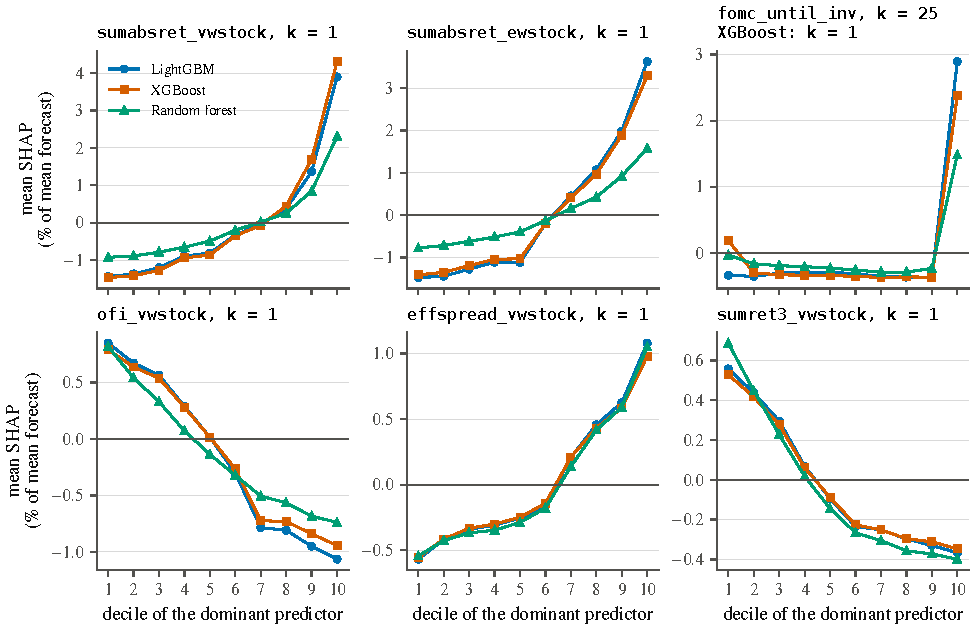
\includegraphics[width=\linewidth]{figures/fi_pooled/fip_shapes.pdf}
\caption{Response shapes of the leading non-standard series. For each series, the mean SHAP value of the series (all its predictors) in each decile of its dominant predictor, the value average at horizon $k$ with the largest mean absolute SHAP value, as a percentage of the mean forecast; over all \rhfipNRows{} bars. The predictor values are the robust-scaled inputs the trees see. A model's line is drawn where the series' share is at least \rhfipShapeMin\% (the classification in Table~\ref{tab:rh_fip_nonstd}); the five series with the largest mean share over the three tree ensembles and the next row of that table.}
\label{fig:rh_fip_shapes}
\end{figure}

% SHAP interactions in LightGBM and XGBoost: shares by class, the largest pairs with a non-standard series
% AUTO-GENERATED by writeup/make_rehaul_fi_pooled.py -- do not edit; re-run the script.
\providecommand{\ser}[2]{#2}\providecommand{\serx}[3]{#3}

\ifdefined\rhfipNOrigins\else% AUTO-GENERATED by writeup/make_rehaul_fi_pooled.py -- do not edit; re-run the script.
\providecommand{\ser}[2]{#2}\providecommand{\serx}[3]{#3}
% \rhfip... macros for writeup/rehaul/08_feature_importance.tex (results/tree_shap_w3000_2014start_fomcfix_2026-10-26, the
% FOMC-patched design, its linear reference inputs/fiw_gamma_fomcfix.npz; the window study's ...W... macros:
% results/fi_by_window_2014start_2026-10-22, pre-patch; the final pooled runs, W = 3,000 trading days).
\providecommand{\rhfipNOrigins}{}\renewcommand{\rhfipNOrigins}{126}  % monthly origins (re-estimations explained)
\providecommand{\rhfipNRows}{}\renewcommand{\rhfipNRows}{33{,}970}  % bars explained, every bar of the evaluation span
\providecommand{\rhfipOriginEvery}{}\renewcommand{\rhfipOriginEvery}{21}  % trading days between origins
\providecommand{\rhfipLastBlock}{}\renewcommand{\rhfipLastBlock}{18}  % trading days of the last origin's block
\providecommand{\rhfipFirstOrigin}{}\renewcommand{\rhfipFirstOrigin}{2~January~2014}  % first origin (10:00 bar)
\providecommand{\rhfipLastOrigin}{}\renewcommand{\rhfipLastOrigin}{5~April~2024}  % last origin
\providecommand{\rhfipLastDay}{}\renewcommand{\rhfipLastDay}{30~April~2024}  % day of the last bar explained
\providecommand{\rhfipWindowDays}{}\renewcommand{\rhfipWindowDays}{3{,}000}  % rolling window, trading days
\providecommand{\rhfipWindowBars}{}\renewcommand{\rhfipWindowBars}{39{,}000}  % rolling window, bars
\providecommand{\rhfipNCols}{}\renewcommand{\rhfipNCols}{564}  % predictors of the full set
\providecommand{\rhfipNGroups}{}\renewcommand{\rhfipNGroups}{48}  % predictor groups: 46 exogenous series + HAR components + calendar dummies
\providecommand{\rhfipNExog}{}\renewcommand{\rhfipNExog}{46}  % exogenous series
\providecommand{\rhfipNPerSeries}{}\renewcommand{\rhfipNPerSeries}{12}  % predictors per exogenous series: value and availability averages at six horizons
\providecommand{\rhfipNStd}{}\renewcommand{\rhfipNStd}{12}  % standard groups
\providecommand{\rhfipNNonStd}{}\renewcommand{\rhfipNNonStd}{36}  % non-standard series
\providecommand{\rhfipNStdExog}{}\renewcommand{\rhfipNStdExog}{10}  % standard exogenous series
\providecommand{\rhfipTuneLast}{}\renewcommand{\rhfipTuneLast}{31~December~2013}  % last day of the last tuning fold (fold 3)
\providecommand{\rhfipRidgePen}{}\renewcommand{\rhfipRidgePen}{\ensuremath{10^{3}}}
\providecommand{\rhfipLassoPen}{}\renewcommand{\rhfipLassoPen}{\ensuremath{10^{-4}}}
\providecommand{\rhfipEnetPen}{}\renewcommand{\rhfipEnetPen}{\ensuremath{10^{-3}}}
\providecommand{\rhfipHarPf}{}\renewcommand{\rhfipHarPf}{0.01}  % penalty factor, HAR block
\providecommand{\rhfipBootBlock}{}\renewcommand{\rhfipBootBlock}{12}  % bootstrap block, origins
\providecommand{\rhfipBootB}{}\renewcommand{\rhfipBootB}{2{,}000}
\providecommand{\rhfipCiLevel}{}\renewcommand{\rhfipCiLevel}{95}  % percentile intervals of both rules (RULE_shap.txt, RULE_fiw.txt)
\providecommand{\rhfipShapeMin}{}\renewcommand{\rhfipShapeMin}{0.5}  % M3 selection: share of at least this many percent
\providecommand{\rhfipTopN}{}\renewcommand{\rhfipTopN}{10}  % length of the top lists compared (m2_rank.csv top10_overlap)
\providecommand{\rhfipSlopeUnit}{}\renewcommand{\rhfipSlopeUnit}{1{,}000}  % trading days per unit of the window slope
\providecommand{\rhfipNMom}{}\renewcommand{\rhfipNMom}{seven}  % the futures' realized moments (standard)
\providecommand{\rhfipLgbmGateEq}{}\renewcommand{\rhfipLgbmGateEq}{126}  % origins bit-equal to the merged every-bar walk
\providecommand{\rhfipXgbGateEq}{}\renewcommand{\rhfipXgbGateEq}{126}  % origins bit-equal to the merged every-bar walk
\providecommand{\rhfipRfGateEq}{}\renewcommand{\rhfipRfGateEq}{126}  % origins bit-equal to the merged every-bar walk
\providecommand{\rhfipRfGateAtShap}{}\renewcommand{\rhfipRfGateAtShap}{126}  % forest origins the walk had written when the SHAP gate ran
\providecommand{\rhfipXgbAddMax}{}\renewcommand{\rhfipXgbAddMax}{\ensuremath{3.7\times 10^{-6}}}  % XGBoost additivity, float32
\providecommand{\rhfipXgbAddTol}{}\renewcommand{\rhfipXgbAddTol}{\ensuremath{10^{-5}}}
\providecommand{\rhfipAddMaxDouble}{}\renewcommand{\rhfipAddMaxDouble}{\ensuremath{5.1\times 10^{-14}}}
\providecommand{\rhfipLinGateMax}{}\renewcommand{\rhfipLinGateMax}{\ensuremath{4.4\times 10^{-16}}}  % linear replay vs walk forecasts, W = 3,000
\providecommand{\rhfipInterRows}{}\renewcommand{\rhfipInterRows}{1{,}008}  % M5 rows
\providecommand{\rhfipInterPerOrigin}{}\renewcommand{\rhfipInterPerOrigin}{8}  % M5 rows per origin
\providecommand{\rhfipFomcRows}{}\renewcommand{\rhfipFomcRows}{1{,}014}
\providecommand{\rhfipFomcDaysShap}{}\renewcommand{\rhfipFomcDaysShap}{78}  % FOMC statement days in the SHAP subset (M4; releases.parquet only)
\providecommand{\rhfipFomcDays}{}\renewcommand{\rhfipFomcDays}{81}  % scheduled FOMC statement days in the span (loader calendar)
\providecommand{\rhfipFomcDaysMissing}{}\renewcommand{\rhfipFomcDaysMissing}{3}  % statement days the SHAP subset leaves out (counted with the other days; the patched rerun's reducer keeps releases.parquet's days)
\providecommand{\rhfipNHolSessions}{}\renewcommand{\rhfipNHolSessions}{64}  % NYSE-holiday futures sessions among the explained bars (not scored in Table 1)
\providecommand{\rhfipNHolBars}{}\renewcommand{\rhfipNHolBars}{443}  % their regular-hours bars
\providecommand{\rhfipVixLo}{}\renewcommand{\rhfipVixLo}{13.96}
\providecommand{\rhfipVixHi}{}\renewcommand{\rhfipVixHi}{19.02}
\providecommand{\rhfipLgbmHar}{}\renewcommand{\rhfipLgbmHar}{51.7}
\providecommand{\rhfipLgbmHarLo}{}\renewcommand{\rhfipLgbmHarLo}{49.5}
\providecommand{\rhfipLgbmHarHi}{}\renewcommand{\rhfipLgbmHarHi}{53.7}
\providecommand{\rhfipLgbmMom}{}\renewcommand{\rhfipLgbmMom}{22.3}
\providecommand{\rhfipLgbmNs}{}\renewcommand{\rhfipLgbmNs}{21.8}
\providecommand{\rhfipLgbmNsLo}{}\renewcommand{\rhfipLgbmNsLo}{20.4}
\providecommand{\rhfipLgbmNsHi}{}\renewcommand{\rhfipLgbmNsHi}{23.4}
\providecommand{\rhfipLgbmNsEx}{}\renewcommand{\rhfipLgbmNsEx}{45.9}
\providecommand{\rhfipLgbmNsExLo}{}\renewcommand{\rhfipLgbmNsExLo}{44.2}
\providecommand{\rhfipLgbmNsExHi}{}\renewcommand{\rhfipLgbmNsExHi}{47.7}
\providecommand{\rhfipXgbHar}{}\renewcommand{\rhfipXgbHar}{52.0}
\providecommand{\rhfipXgbHarLo}{}\renewcommand{\rhfipXgbHarLo}{50.0}
\providecommand{\rhfipXgbHarHi}{}\renewcommand{\rhfipXgbHarHi}{53.8}
\providecommand{\rhfipXgbMom}{}\renewcommand{\rhfipXgbMom}{23.6}
\providecommand{\rhfipXgbNs}{}\renewcommand{\rhfipXgbNs}{20.6}
\providecommand{\rhfipXgbNsLo}{}\renewcommand{\rhfipXgbNsLo}{19.2}
\providecommand{\rhfipXgbNsHi}{}\renewcommand{\rhfipXgbNsHi}{22.2}
\providecommand{\rhfipXgbNsEx}{}\renewcommand{\rhfipXgbNsEx}{43.6}
\providecommand{\rhfipXgbNsExLo}{}\renewcommand{\rhfipXgbNsExLo}{41.8}
\providecommand{\rhfipXgbNsExHi}{}\renewcommand{\rhfipXgbNsExHi}{45.7}
\providecommand{\rhfipRfHar}{}\renewcommand{\rhfipRfHar}{57.6}
\providecommand{\rhfipRfHarLo}{}\renewcommand{\rhfipRfHarLo}{55.4}
\providecommand{\rhfipRfHarHi}{}\renewcommand{\rhfipRfHarHi}{59.6}
\providecommand{\rhfipRfMom}{}\renewcommand{\rhfipRfMom}{20.7}
\providecommand{\rhfipRfNs}{}\renewcommand{\rhfipRfNs}{18.6}
\providecommand{\rhfipRfNsLo}{}\renewcommand{\rhfipRfNsLo}{17.2}
\providecommand{\rhfipRfNsHi}{}\renewcommand{\rhfipRfNsHi}{20.3}
\providecommand{\rhfipRfNsEx}{}\renewcommand{\rhfipRfNsEx}{44.2}
\providecommand{\rhfipRfNsExLo}{}\renewcommand{\rhfipRfNsExLo}{42.1}
\providecommand{\rhfipRfNsExHi}{}\renewcommand{\rhfipRfNsExHi}{46.5}
\providecommand{\rhfipRidgeNsEx}{}\renewcommand{\rhfipRidgeNsEx}{68.8}
\providecommand{\rhfipRidgeNs}{}\renewcommand{\rhfipRidgeNs}{55.6}
\providecommand{\rhfipRidgeHar}{}\renewcommand{\rhfipRidgeHar}{17.5}
\providecommand{\rhfipLassoNsEx}{}\renewcommand{\rhfipLassoNsEx}{82.5}
\providecommand{\rhfipLassoNs}{}\renewcommand{\rhfipLassoNs}{76.5}
\providecommand{\rhfipLassoHar}{}\renewcommand{\rhfipLassoHar}{6.7}
\providecommand{\rhfipEnetNsEx}{}\renewcommand{\rhfipEnetNsEx}{60.0}
\providecommand{\rhfipEnetNs}{}\renewcommand{\rhfipEnetNs}{42.9}
\providecommand{\rhfipEnetHar}{}\renewcommand{\rhfipEnetHar}{26.4}
\providecommand{\rhfipHarMin}{}\renewcommand{\rhfipHarMin}{51.7}
\providecommand{\rhfipHarMax}{}\renewcommand{\rhfipHarMax}{57.6}
\providecommand{\rhfipMomMin}{}\renewcommand{\rhfipMomMin}{20.7}
\providecommand{\rhfipMomMax}{}\renewcommand{\rhfipMomMax}{23.6}
\providecommand{\rhfipNsExMin}{}\renewcommand{\rhfipNsExMin}{43.6}
\providecommand{\rhfipNsExMax}{}\renewcommand{\rhfipNsExMax}{45.9}
\providecommand{\rhfipSentMin}{}\renewcommand{\rhfipSentMin}{0.6}
\providecommand{\rhfipSentMax}{}\renewcommand{\rhfipSentMax}{0.8}
\providecommand{\rhfipVdMin}{}\renewcommand{\rhfipVdMin}{0.2}
\providecommand{\rhfipVdMax}{}\renewcommand{\rhfipVdMax}{0.3}
\providecommand{\rhfipFomcBucketMin}{}\renewcommand{\rhfipFomcBucketMin}{1.4}
\providecommand{\rhfipFomcBucketMax}{}\renewcommand{\rhfipFomcBucketMax}{2.3}
\providecommand{\rhfipVvixMin}{}\renewcommand{\rhfipVvixMin}{0.2}
\providecommand{\rhfipVvixMax}{}\renewcommand{\rhfipVvixMax}{0.3}
\providecommand{\rhfipVixThreeMMin}{}\renewcommand{\rhfipVixThreeMMin}{0.3}
\providecommand{\rhfipVixThreeMMax}{}\renewcommand{\rhfipVixThreeMMax}{0.7}
\providecommand{\rhfipFomcDayMin}{}\renewcommand{\rhfipFomcDayMin}{0.1}
\providecommand{\rhfipFomcDayMax}{}\renewcommand{\rhfipFomcDayMax}{0.1}
\providecommand{\rhfipNsOne}{}\renewcommand{\rhfipNsOne}{\ensuremath{\ser{sumabsret_vwstock}{\mathrm{RAV}^{\mathrm{VW}}}}}
\providecommand{\rhfipNsOneMin}{}\renewcommand{\rhfipNsOneMin}{2.4}
\providecommand{\rhfipNsOneMax}{}\renewcommand{\rhfipNsOneMax}{3.9}
\providecommand{\rhfipNsOneLgbm}{}\renewcommand{\rhfipNsOneLgbm}{3.5}
\providecommand{\rhfipNsOneXgb}{}\renewcommand{\rhfipNsOneXgb}{3.9}
\providecommand{\rhfipNsOneRf}{}\renewcommand{\rhfipNsOneRf}{2.4}
\providecommand{\rhfipNsTwo}{}\renewcommand{\rhfipNsTwo}{\ensuremath{\ser{sumabsret_ewstock}{\mathrm{RAV}^{\mathrm{EW}}}}}
\providecommand{\rhfipNsTwoMin}{}\renewcommand{\rhfipNsTwoMin}{1.9}
\providecommand{\rhfipNsTwoMax}{}\renewcommand{\rhfipNsTwoMax}{3.9}
\providecommand{\rhfipNsTwoLgbm}{}\renewcommand{\rhfipNsTwoLgbm}{3.9}
\providecommand{\rhfipNsTwoXgb}{}\renewcommand{\rhfipNsTwoXgb}{3.8}
\providecommand{\rhfipNsTwoRf}{}\renewcommand{\rhfipNsTwoRf}{1.9}
\providecommand{\rhfipNsThree}{}\renewcommand{\rhfipNsThree}{\ensuremath{\ser{fomc_until_inv}{\mathrm{FOMC}^{\mathrm{next}}}}}
\providecommand{\rhfipNsThreeMin}{}\renewcommand{\rhfipNsThreeMin}{1.1}
\providecommand{\rhfipNsThreeMax}{}\renewcommand{\rhfipNsThreeMax}{2.0}
\providecommand{\rhfipNsThreeLgbm}{}\renewcommand{\rhfipNsThreeLgbm}{2.0}
\providecommand{\rhfipNsThreeXgb}{}\renewcommand{\rhfipNsThreeXgb}{2.0}
\providecommand{\rhfipNsThreeRf}{}\renewcommand{\rhfipNsThreeRf}{1.1}
\providecommand{\rhfipNsFour}{}\renewcommand{\rhfipNsFour}{\ensuremath{\ser{ofi_vwstock}{\mathrm{OFI}^{\mathrm{VW}}}}}
\providecommand{\rhfipNsFourMin}{}\renewcommand{\rhfipNsFourMin}{1.4}
\providecommand{\rhfipNsFourMax}{}\renewcommand{\rhfipNsFourMax}{1.8}
\providecommand{\rhfipNsFourLgbm}{}\renewcommand{\rhfipNsFourLgbm}{1.8}
\providecommand{\rhfipNsFourXgb}{}\renewcommand{\rhfipNsFourXgb}{1.7}
\providecommand{\rhfipNsFourRf}{}\renewcommand{\rhfipNsFourRf}{1.4}
\providecommand{\rhfipNsFive}{}\renewcommand{\rhfipNsFive}{\ensuremath{\ser{effspread_vwstock}{\mathrm{EffSpread}^{\mathrm{VW}}}}}
\providecommand{\rhfipNsFiveMin}{}\renewcommand{\rhfipNsFiveMin}{1.2}
\providecommand{\rhfipNsFiveMax}{}\renewcommand{\rhfipNsFiveMax}{1.3}
\providecommand{\rhfipNsFiveLgbm}{}\renewcommand{\rhfipNsFiveLgbm}{1.2}
\providecommand{\rhfipNsFiveXgb}{}\renewcommand{\rhfipNsFiveXgb}{1.2}
\providecommand{\rhfipNsFiveRf}{}\renewcommand{\rhfipNsFiveRf}{1.3}
\providecommand{\rhfipTreeTopOne}{}\renewcommand{\rhfipTreeTopOne}{\ensuremath{\ser{sumabsret}{\mathrm{RAV}}}}
\providecommand{\rhfipTreeTopTwo}{}\renewcommand{\rhfipTreeTopTwo}{\ensuremath{\ser{sumret}{r}}}
\providecommand{\rhfipLgbmTopOneEx}{}\renewcommand{\rhfipLgbmTopOneEx}{20.3}
\providecommand{\rhfipXgbTopOneEx}{}\renewcommand{\rhfipXgbTopOneEx}{24.7}
\providecommand{\rhfipRfTopOneEx}{}\renewcommand{\rhfipRfTopOneEx}{29.2}
\providecommand{\rhfipRidgeTopOne}{}\renewcommand{\rhfipRidgeTopOne}{\ensuremath{\ser{fomc_until_inv}{\mathrm{FOMC}^{\mathrm{next}}}}}
\providecommand{\rhfipRidgeTopOneEx}{}\renewcommand{\rhfipRidgeTopOneEx}{9.0}
\providecommand{\rhfipLgbmNUsedAll}{}\renewcommand{\rhfipLgbmNUsedAll}{42}  % exogenous series split on at every origin
\providecommand{\rhfipLgbmUsedMin}{}\renewcommand{\rhfipLgbmUsedMin}{58}
\providecommand{\rhfipXgbNUsedAll}{}\renewcommand{\rhfipXgbNUsedAll}{43}  % exogenous series split on at every origin
\providecommand{\rhfipXgbUsedMin}{}\renewcommand{\rhfipXgbUsedMin}{72}
\providecommand{\rhfipRfNUsedAll}{}\renewcommand{\rhfipRfNUsedAll}{46}  % exogenous series split on at every origin
\providecommand{\rhfipRfUsedMin}{}\renewcommand{\rhfipRfUsedMin}{126}
\providecommand{\rhfipLgbmDRidge}{}\renewcommand{\rhfipLgbmDRidge}{\ensuremath{-}22.9}
\providecommand{\rhfipLgbmDRidgeLo}{}\renewcommand{\rhfipLgbmDRidgeLo}{\ensuremath{-}24.8}
\providecommand{\rhfipLgbmDRidgeHi}{}\renewcommand{\rhfipLgbmDRidgeHi}{\ensuremath{-}21.1}
\providecommand{\rhfipLgbmDLasso}{}\renewcommand{\rhfipLgbmDLasso}{\ensuremath{-}36.6}
\providecommand{\rhfipLgbmDLassoLo}{}\renewcommand{\rhfipLgbmDLassoLo}{\ensuremath{-}39.1}
\providecommand{\rhfipLgbmDLassoHi}{}\renewcommand{\rhfipLgbmDLassoHi}{\ensuremath{-}34.4}
\providecommand{\rhfipLgbmDEnet}{}\renewcommand{\rhfipLgbmDEnet}{\ensuremath{-}14.1}
\providecommand{\rhfipLgbmDEnetLo}{}\renewcommand{\rhfipLgbmDEnetLo}{\ensuremath{-}15.7}
\providecommand{\rhfipLgbmDEnetHi}{}\renewcommand{\rhfipLgbmDEnetHi}{\ensuremath{-}12.7}
\providecommand{\rhfipXgbDRidge}{}\renewcommand{\rhfipXgbDRidge}{\ensuremath{-}25.1}
\providecommand{\rhfipXgbDRidgeLo}{}\renewcommand{\rhfipXgbDRidgeLo}{\ensuremath{-}27.0}
\providecommand{\rhfipXgbDRidgeHi}{}\renewcommand{\rhfipXgbDRidgeHi}{\ensuremath{-}23.3}
\providecommand{\rhfipXgbDLasso}{}\renewcommand{\rhfipXgbDLasso}{\ensuremath{-}38.9}
\providecommand{\rhfipXgbDLassoLo}{}\renewcommand{\rhfipXgbDLassoLo}{\ensuremath{-}41.4}
\providecommand{\rhfipXgbDLassoHi}{}\renewcommand{\rhfipXgbDLassoHi}{\ensuremath{-}36.6}
\providecommand{\rhfipXgbDEnet}{}\renewcommand{\rhfipXgbDEnet}{\ensuremath{-}16.3}
\providecommand{\rhfipXgbDEnetLo}{}\renewcommand{\rhfipXgbDEnetLo}{\ensuremath{-}17.8}
\providecommand{\rhfipXgbDEnetHi}{}\renewcommand{\rhfipXgbDEnetHi}{\ensuremath{-}14.9}
\providecommand{\rhfipRfDRidge}{}\renewcommand{\rhfipRfDRidge}{\ensuremath{-}24.5}
\providecommand{\rhfipRfDRidgeLo}{}\renewcommand{\rhfipRfDRidgeLo}{\ensuremath{-}26.3}
\providecommand{\rhfipRfDRidgeHi}{}\renewcommand{\rhfipRfDRidgeHi}{\ensuremath{-}22.9}
\providecommand{\rhfipRfDLasso}{}\renewcommand{\rhfipRfDLasso}{\ensuremath{-}38.3}
\providecommand{\rhfipRfDLassoLo}{}\renewcommand{\rhfipRfDLassoLo}{\ensuremath{-}40.5}
\providecommand{\rhfipRfDLassoHi}{}\renewcommand{\rhfipRfDLassoHi}{\ensuremath{-}36.3}
\providecommand{\rhfipRfDEnet}{}\renewcommand{\rhfipRfDEnet}{\ensuremath{-}15.7}
\providecommand{\rhfipRfDEnetLo}{}\renewcommand{\rhfipRfDEnetLo}{\ensuremath{-}17.0}
\providecommand{\rhfipRfDEnetHi}{}\renewcommand{\rhfipRfDEnetHi}{\ensuremath{-}14.4}
\providecommand{\rhfipNDLess}{}\renewcommand{\rhfipNDLess}{27}  % tree-minus-linear D with the 95% interval below 0
\providecommand{\rhfipNDAll}{}\renewcommand{\rhfipNDAll}{27}  % D comparisons: 3 trees x 3 linear models x 3 denominators
\providecommand{\rhfipLgbmSpRidge}{}\renewcommand{\rhfipLgbmSpRidge}{0.57}
\providecommand{\rhfipLgbmTopRidge}{}\renewcommand{\rhfipLgbmTopRidge}{6}
\providecommand{\rhfipLgbmSpLasso}{}\renewcommand{\rhfipLgbmSpLasso}{0.49}
\providecommand{\rhfipLgbmTopLasso}{}\renewcommand{\rhfipLgbmTopLasso}{5}
\providecommand{\rhfipLgbmSpEnet}{}\renewcommand{\rhfipLgbmSpEnet}{0.66}
\providecommand{\rhfipLgbmTopEnet}{}\renewcommand{\rhfipLgbmTopEnet}{6}
\providecommand{\rhfipXgbSpRidge}{}\renewcommand{\rhfipXgbSpRidge}{0.55}
\providecommand{\rhfipXgbTopRidge}{}\renewcommand{\rhfipXgbTopRidge}{6}
\providecommand{\rhfipXgbSpLasso}{}\renewcommand{\rhfipXgbSpLasso}{0.47}
\providecommand{\rhfipXgbTopLasso}{}\renewcommand{\rhfipXgbTopLasso}{5}
\providecommand{\rhfipXgbSpEnet}{}\renewcommand{\rhfipXgbSpEnet}{0.63}
\providecommand{\rhfipXgbTopEnet}{}\renewcommand{\rhfipXgbTopEnet}{6}
\providecommand{\rhfipRfSpRidge}{}\renewcommand{\rhfipRfSpRidge}{0.53}
\providecommand{\rhfipRfTopRidge}{}\renewcommand{\rhfipRfTopRidge}{5}
\providecommand{\rhfipRfSpLasso}{}\renewcommand{\rhfipRfSpLasso}{0.43}
\providecommand{\rhfipRfTopLasso}{}\renewcommand{\rhfipRfTopLasso}{4}
\providecommand{\rhfipRfSpEnet}{}\renewcommand{\rhfipRfSpEnet}{0.60}
\providecommand{\rhfipRfTopEnet}{}\renewcommand{\rhfipRfTopEnet}{5}
\providecommand{\rhfipSpLgbmXgb}{}\renewcommand{\rhfipSpLgbmXgb}{0.99}
\providecommand{\rhfipSpLgbmRf}{}\renewcommand{\rhfipSpLgbmRf}{0.90}
\providecommand{\rhfipSpXgbRf}{}\renewcommand{\rhfipSpXgbRf}{0.89}
\providecommand{\rhfipRidgeRankFomcUntil}{}\renewcommand{\rhfipRidgeRankFomcUntil}{1}
\providecommand{\rhfipTreeRankFomcUntilMin}{}\renewcommand{\rhfipTreeRankFomcUntilMin}{6}
\providecommand{\rhfipTreeRankFomcUntilMax}{}\renewcommand{\rhfipTreeRankFomcUntilMax}{10}
\providecommand{\rhfipRidgeRankFomcDay}{}\renewcommand{\rhfipRidgeRankFomcDay}{9}
\providecommand{\rhfipTreeRankFomcDayMin}{}\renewcommand{\rhfipTreeRankFomcDayMin}{39}
\providecommand{\rhfipTreeRankFomcDayMax}{}\renewcommand{\rhfipTreeRankFomcDayMax}{43}
\providecommand{\rhfipFomcUntil}{}\renewcommand{\rhfipFomcUntil}{\ensuremath{\ser{fomc_until_inv}{\mathrm{FOMC}^{\mathrm{next}}}}}
\providecommand{\rhfipFomcDay}{}\renewcommand{\rhfipFomcDay}{\ensuremath{\ser{fomc_day}{\mathrm{FOMC}^{\mathrm{day}}}}}
\providecommand{\rhfipAbsVw}{}\renewcommand{\rhfipAbsVw}{\ensuremath{\ser{sumabsret_vwstock}{\mathrm{RAV}^{\mathrm{VW}}}}}
\providecommand{\rhfipOfi}{}\renewcommand{\rhfipOfi}{\ensuremath{\ser{ofi_vwstock}{\mathrm{OFI}^{\mathrm{VW}}}}}
\providecommand{\rhfipLgbmNeff}{}\renewcommand{\rhfipLgbmNeff}{11.0}
\providecommand{\rhfipLgbmNHalf}{}\renewcommand{\rhfipLgbmNHalf}{4}
\providecommand{\rhfipLgbmNEighty}{}\renewcommand{\rhfipLgbmNEighty}{13}
\providecommand{\rhfipXgbNeff}{}\renewcommand{\rhfipXgbNeff}{9.1}
\providecommand{\rhfipXgbNHalf}{}\renewcommand{\rhfipXgbNHalf}{4}
\providecommand{\rhfipXgbNEighty}{}\renewcommand{\rhfipXgbNEighty}{11}
\providecommand{\rhfipRfNeff}{}\renewcommand{\rhfipRfNeff}{8.9}
\providecommand{\rhfipRfNHalf}{}\renewcommand{\rhfipRfNHalf}{4}
\providecommand{\rhfipRfNEighty}{}\renewcommand{\rhfipRfNEighty}{16}
\providecommand{\rhfipRidgeNeff}{}\renewcommand{\rhfipRidgeNeff}{28.5}
\providecommand{\rhfipRidgeNHalf}{}\renewcommand{\rhfipRidgeNHalf}{11}
\providecommand{\rhfipRidgeNEighty}{}\renewcommand{\rhfipRidgeNEighty}{26}
\providecommand{\rhfipLassoNeff}{}\renewcommand{\rhfipLassoNeff}{5.1}
\providecommand{\rhfipLassoNHalf}{}\renewcommand{\rhfipLassoNHalf}{2}
\providecommand{\rhfipLassoNEighty}{}\renewcommand{\rhfipLassoNEighty}{11}
\providecommand{\rhfipEnetNeff}{}\renewcommand{\rhfipEnetNeff}{16.2}
\providecommand{\rhfipEnetNHalf}{}\renewcommand{\rhfipEnetNHalf}{6}
\providecommand{\rhfipEnetNEighty}{}\renewcommand{\rhfipEnetNEighty}{15}
\providecommand{\rhfipYearFirst}{}\renewcommand{\rhfipYearFirst}{2014}
\providecommand{\rhfipYearLast}{}\renewcommand{\rhfipYearLast}{2024}
\providecommand{\rhfipLgbmNsYearMin}{}\renewcommand{\rhfipLgbmNsYearMin}{18.1}
\providecommand{\rhfipLgbmNsYearMinYr}{}\renewcommand{\rhfipLgbmNsYearMinYr}{2021}
\providecommand{\rhfipLgbmNsYearMax}{}\renewcommand{\rhfipLgbmNsYearMax}{25.6}
\providecommand{\rhfipLgbmNsYearMaxYr}{}\renewcommand{\rhfipLgbmNsYearMaxYr}{2015}
\providecommand{\rhfipLgbmHarYearMax}{}\renewcommand{\rhfipLgbmHarYearMax}{57.4}
\providecommand{\rhfipLgbmHarYearMaxYr}{}\renewcommand{\rhfipLgbmHarYearMaxYr}{2021}
\providecommand{\rhfipLgbmHarYearMin}{}\renewcommand{\rhfipLgbmHarYearMin}{44.6}
\providecommand{\rhfipLgbmHarYearMinYr}{}\renewcommand{\rhfipLgbmHarYearMinYr}{2017}
\providecommand{\rhfipXgbNsYearMin}{}\renewcommand{\rhfipXgbNsYearMin}{17.2}
\providecommand{\rhfipXgbNsYearMinYr}{}\renewcommand{\rhfipXgbNsYearMinYr}{2021}
\providecommand{\rhfipXgbNsYearMax}{}\renewcommand{\rhfipXgbNsYearMax}{24.3}
\providecommand{\rhfipXgbNsYearMaxYr}{}\renewcommand{\rhfipXgbNsYearMaxYr}{2015}
\providecommand{\rhfipXgbHarYearMax}{}\renewcommand{\rhfipXgbHarYearMax}{57.0}
\providecommand{\rhfipXgbHarYearMaxYr}{}\renewcommand{\rhfipXgbHarYearMaxYr}{2021}
\providecommand{\rhfipXgbHarYearMin}{}\renewcommand{\rhfipXgbHarYearMin}{45.8}
\providecommand{\rhfipXgbHarYearMinYr}{}\renewcommand{\rhfipXgbHarYearMinYr}{2017}
\providecommand{\rhfipRfNsYearMin}{}\renewcommand{\rhfipRfNsYearMin}{15.2}
\providecommand{\rhfipRfNsYearMinYr}{}\renewcommand{\rhfipRfNsYearMinYr}{2021}
\providecommand{\rhfipRfNsYearMax}{}\renewcommand{\rhfipRfNsYearMax}{22.9}
\providecommand{\rhfipRfNsYearMaxYr}{}\renewcommand{\rhfipRfNsYearMaxYr}{2015}
\providecommand{\rhfipRfHarYearMax}{}\renewcommand{\rhfipRfHarYearMax}{62.3}
\providecommand{\rhfipRfHarYearMaxYr}{}\renewcommand{\rhfipRfHarYearMaxYr}{2019}
\providecommand{\rhfipRfHarYearMin}{}\renewcommand{\rhfipRfHarYearMin}{50.4}
\providecommand{\rhfipRfHarYearMinYr}{}\renewcommand{\rhfipRfHarYearMinYr}{2017}
\providecommand{\rhfipNsYearMinYr}{}\renewcommand{\rhfipNsYearMinYr}{2021}  % the year of every tree's lowest non-standard share
\providecommand{\rhfipDipFirst}{}\renewcommand{\rhfipDipFirst}{2018}  % first of the years in which every tree's non-standard share is below its pooled share
\providecommand{\rhfipDipLast}{}\renewcommand{\rhfipDipLast}{2022}
\providecommand{\rhfipRidgeNsExYearMin}{}\renewcommand{\rhfipRidgeNsExYearMin}{65.1}
\providecommand{\rhfipRidgeNsExYearMinYr}{}\renewcommand{\rhfipRidgeNsExYearMinYr}{2021}
\providecommand{\rhfipRidgeNsExYearMax}{}\renewcommand{\rhfipRidgeNsExYearMax}{72.4}
\providecommand{\rhfipRidgeNsExYearMaxYr}{}\renewcommand{\rhfipRidgeNsExYearMaxYr}{2017}
\providecommand{\rhfipLassoNsExYearMin}{}\renewcommand{\rhfipLassoNsExYearMin}{77.1}
\providecommand{\rhfipLassoNsExYearMinYr}{}\renewcommand{\rhfipLassoNsExYearMinYr}{2021}
\providecommand{\rhfipLassoNsExYearMax}{}\renewcommand{\rhfipLassoNsExYearMax}{87.1}
\providecommand{\rhfipLassoNsExYearMaxYr}{}\renewcommand{\rhfipLassoNsExYearMaxYr}{2017}
\providecommand{\rhfipEnetNsExYearMin}{}\renewcommand{\rhfipEnetNsExYearMin}{56.1}
\providecommand{\rhfipEnetNsExYearMinYr}{}\renewcommand{\rhfipEnetNsExYearMinYr}{2019}
\providecommand{\rhfipEnetNsExYearMax}{}\renewcommand{\rhfipEnetNsExYearMax}{65.2}
\providecommand{\rhfipEnetNsExYearMaxYr}{}\renewcommand{\rhfipEnetNsExYearMaxYr}{2014}
\providecommand{\rhfipLgbmNsExYearMin}{}\renewcommand{\rhfipLgbmNsExYearMin}{42.3}
\providecommand{\rhfipLgbmNsExYearMax}{}\renewcommand{\rhfipLgbmNsExYearMax}{50.1}
\providecommand{\rhfipXgbNsExYearMin}{}\renewcommand{\rhfipXgbNsExYearMin}{39.4}
\providecommand{\rhfipXgbNsExYearMax}{}\renewcommand{\rhfipXgbNsExYearMax}{48.9}
\providecommand{\rhfipRfNsExYearMin}{}\renewcommand{\rhfipRfNsExYearMin}{39.5}
\providecommand{\rhfipRfNsExYearMax}{}\renewcommand{\rhfipRfNsExYearMax}{50.9}
\providecommand{\rhfipLgbmNShape}{}\renewcommand{\rhfipLgbmNShape}{11}  % non-standard series at >= 0.5% (M3)
\providecommand{\rhfipLgbmNMono}{}\renewcommand{\rhfipLgbmNMono}{7}
\providecommand{\rhfipLgbmNIrr}{}\renewcommand{\rhfipLgbmNIrr}{3}
\providecommand{\rhfipLgbmNStep}{}\renewcommand{\rhfipLgbmNStep}{1}
\providecommand{\rhfipLgbmNFlat}{}\renewcommand{\rhfipLgbmNFlat}{0}
\providecommand{\rhfipLgbmNThresh}{}\renewcommand{\rhfipLgbmNThresh}{0}
\providecommand{\rhfipLgbmNU}{}\renewcommand{\rhfipLgbmNU}{0}
\providecommand{\rhfipLgbmNAsym}{}\renewcommand{\rhfipLgbmNAsym}{9}
\providecommand{\rhfipXgbNShape}{}\renewcommand{\rhfipXgbNShape}{10}  % non-standard series at >= 0.5% (M3)
\providecommand{\rhfipXgbNMono}{}\renewcommand{\rhfipXgbNMono}{5}
\providecommand{\rhfipXgbNIrr}{}\renewcommand{\rhfipXgbNIrr}{3}
\providecommand{\rhfipXgbNStep}{}\renewcommand{\rhfipXgbNStep}{0}
\providecommand{\rhfipXgbNFlat}{}\renewcommand{\rhfipXgbNFlat}{1}
\providecommand{\rhfipXgbNThresh}{}\renewcommand{\rhfipXgbNThresh}{1}
\providecommand{\rhfipXgbNU}{}\renewcommand{\rhfipXgbNU}{0}
\providecommand{\rhfipXgbNAsym}{}\renewcommand{\rhfipXgbNAsym}{8}
\providecommand{\rhfipRfNShape}{}\renewcommand{\rhfipRfNShape}{13}  % non-standard series at >= 0.5% (M3)
\providecommand{\rhfipRfNMono}{}\renewcommand{\rhfipRfNMono}{10}
\providecommand{\rhfipRfNIrr}{}\renewcommand{\rhfipRfNIrr}{3}
\providecommand{\rhfipRfNStep}{}\renewcommand{\rhfipRfNStep}{0}
\providecommand{\rhfipRfNFlat}{}\renewcommand{\rhfipRfNFlat}{0}
\providecommand{\rhfipRfNThresh}{}\renewcommand{\rhfipRfNThresh}{0}
\providecommand{\rhfipRfNU}{}\renewcommand{\rhfipRfNU}{0}
\providecommand{\rhfipRfNAsym}{}\renewcommand{\rhfipRfNAsym}{13}
\providecommand{\rhfipNUThreshAll}{}\renewcommand{\rhfipNUThreshAll}{1}  % U-shaped, inverted-U or threshold profiles in any tree
\providecommand{\rhfipAbsVwLgbmLo}{}\renewcommand{\rhfipAbsVwLgbmLo}{\ensuremath{-}1.4}
\providecommand{\rhfipAbsVwLgbmHi}{}\renewcommand{\rhfipAbsVwLgbmHi}{3.9}
\providecommand{\rhfipAbsVwXgbLo}{}\renewcommand{\rhfipAbsVwXgbLo}{\ensuremath{-}1.5}
\providecommand{\rhfipAbsVwXgbHi}{}\renewcommand{\rhfipAbsVwXgbHi}{4.3}
\providecommand{\rhfipAbsVwRfLo}{}\renewcommand{\rhfipAbsVwRfLo}{\ensuremath{-}0.9}
\providecommand{\rhfipAbsVwRfHi}{}\renewcommand{\rhfipAbsVwRfHi}{2.3}
\providecommand{\rhfipOfiLgbmLo}{}\renewcommand{\rhfipOfiLgbmLo}{0.8}
\providecommand{\rhfipOfiLgbmHi}{}\renewcommand{\rhfipOfiLgbmHi}{\ensuremath{-}1.1}
\providecommand{\rhfipOfiXgbLo}{}\renewcommand{\rhfipOfiXgbLo}{0.8}
\providecommand{\rhfipOfiXgbHi}{}\renewcommand{\rhfipOfiXgbHi}{\ensuremath{-}0.9}
\providecommand{\rhfipOfiRfLo}{}\renewcommand{\rhfipOfiRfLo}{0.8}
\providecommand{\rhfipOfiRfHi}{}\renewcommand{\rhfipOfiRfHi}{\ensuremath{-}0.7}
\providecommand{\rhfipUntilLgbmLo}{}\renewcommand{\rhfipUntilLgbmLo}{\ensuremath{-}0.3}
\providecommand{\rhfipUntilLgbmHi}{}\renewcommand{\rhfipUntilLgbmHi}{2.9}
\providecommand{\rhfipUntilXgbLo}{}\renewcommand{\rhfipUntilXgbLo}{0.2}
\providecommand{\rhfipUntilXgbHi}{}\renewcommand{\rhfipUntilXgbHi}{2.4}
\providecommand{\rhfipUntilRfLo}{}\renewcommand{\rhfipUntilRfLo}{\ensuremath{-}0.0}
\providecommand{\rhfipUntilRfHi}{}\renewcommand{\rhfipUntilRfHi}{1.5}
\providecommand{\rhfipUntilHorizon}{}\renewcommand{\rhfipUntilHorizon}{25}  % horizon of fomc_until_inv's dominant column
\providecommand{\rhfipUntilHorizonXgb}{}\renewcommand{\rhfipUntilHorizonXgb}{1}  % the same in XGBoost (differs from the other trees')
\providecommand{\rhfipBarFirst}{}\renewcommand{\rhfipBarFirst}{10:00}
\providecommand{\rhfipBarLast}{}\renewcommand{\rhfipBarLast}{16:00}
\providecommand{\rhfipBarPeakA}{}\renewcommand{\rhfipBarPeakA}{14:30}
\providecommand{\rhfipBarPeakB}{}\renewcommand{\rhfipBarPeakB}{15:00}
\providecommand{\rhfipNBars}{}\renewcommand{\rhfipNBars}{13}
\providecommand{\rhfipLgbmNsFomc}{}\renewcommand{\rhfipLgbmNsFomc}{42.6}
\providecommand{\rhfipLgbmNsOther}{}\renewcommand{\rhfipLgbmNsOther}{20.9}
\providecommand{\rhfipLgbmUntilFomc}{}\renewcommand{\rhfipLgbmUntilFomc}{25.4}
\providecommand{\rhfipLgbmUntilOther}{}\renewcommand{\rhfipLgbmUntilOther}{1.06}
\providecommand{\rhfipLgbmFomcBucketFomc}{}\renewcommand{\rhfipLgbmFomcBucketFomc}{27.3}
\providecommand{\rhfipLgbmFomcBucketOther}{}\renewcommand{\rhfipLgbmFomcBucketOther}{1.3}
\providecommand{\rhfipLgbmHarFomc}{}\renewcommand{\rhfipLgbmHarFomc}{39.2}
\providecommand{\rhfipLgbmHarOther}{}\renewcommand{\rhfipLgbmHarOther}{52.2}
\providecommand{\rhfipLgbmNsFirstBar}{}\renewcommand{\rhfipLgbmNsFirstBar}{23.9}
\providecommand{\rhfipLgbmNsLastBar}{}\renewcommand{\rhfipLgbmNsLastBar}{20.5}
\providecommand{\rhfipLgbmNsAftMin}{}\renewcommand{\rhfipLgbmNsAftMin}{24.3}
\providecommand{\rhfipLgbmNsAftMax}{}\renewcommand{\rhfipLgbmNsAftMax}{25.2}
\providecommand{\rhfipLgbmNsMidMin}{}\renewcommand{\rhfipLgbmNsMidMin}{20.1}
\providecommand{\rhfipLgbmNsMidMax}{}\renewcommand{\rhfipLgbmNsMidMax}{21.9}
\providecommand{\rhfipLgbmFomcBucketAft}{}\renewcommand{\rhfipLgbmFomcBucketAft}{5.5}
\providecommand{\rhfipLgbmFomcBucketOtherBars}{}\renewcommand{\rhfipLgbmFomcBucketOtherBars}{1.4}  % median FOMC-announcement share over the other 11 bars
\providecommand{\rhfipLgbmFomcDiff}{}\renewcommand{\rhfipLgbmFomcDiff}{\ensuremath{+}21.7}
\providecommand{\rhfipLgbmFomcDiffLo}{}\renewcommand{\rhfipLgbmFomcDiffLo}{\ensuremath{+}19.3}
\providecommand{\rhfipLgbmFomcDiffHi}{}\renewcommand{\rhfipLgbmFomcDiffHi}{\ensuremath{+}24.1}
\providecommand{\rhfipLgbmLateDiff}{}\renewcommand{\rhfipLgbmLateDiff}{\ensuremath{-}3.4}
\providecommand{\rhfipLgbmLateDiffLo}{}\renewcommand{\rhfipLgbmLateDiffLo}{\ensuremath{-}4.3}
\providecommand{\rhfipLgbmLateDiffHi}{}\renewcommand{\rhfipLgbmLateDiffHi}{\ensuremath{-}2.5}
\providecommand{\rhfipLgbmVixDiff}{}\renewcommand{\rhfipLgbmVixDiff}{\ensuremath{-}3.2}
\providecommand{\rhfipLgbmVixDiffLo}{}\renewcommand{\rhfipLgbmVixDiffLo}{\ensuremath{-}5.3}
\providecommand{\rhfipLgbmVixDiffHi}{}\renewcommand{\rhfipLgbmVixDiffHi}{\ensuremath{-}1.1}
\providecommand{\rhfipLgbmVixHar}{}\renewcommand{\rhfipLgbmVixHar}{\ensuremath{+}5.1}
\providecommand{\rhfipLgbmVixHarLo}{}\renewcommand{\rhfipLgbmVixHarLo}{\ensuremath{+}1.8}
\providecommand{\rhfipLgbmVixHarHi}{}\renewcommand{\rhfipLgbmVixHarHi}{\ensuremath{+}8.4}
\providecommand{\rhfipLgbmVixDiffEx}{}\renewcommand{\rhfipLgbmVixDiffEx}{\ensuremath{-}2.3}
\providecommand{\rhfipLgbmVixDiffExLo}{}\renewcommand{\rhfipLgbmVixDiffExLo}{\ensuremath{-}4.5}
\providecommand{\rhfipLgbmVixDiffExHi}{}\renewcommand{\rhfipLgbmVixDiffExHi}{\ensuremath{-}0.2}
\providecommand{\rhfipXgbNsFomc}{}\renewcommand{\rhfipXgbNsFomc}{41.1}
\providecommand{\rhfipXgbNsOther}{}\renewcommand{\rhfipXgbNsOther}{19.7}
\providecommand{\rhfipXgbUntilFomc}{}\renewcommand{\rhfipXgbUntilFomc}{23.9}
\providecommand{\rhfipXgbUntilOther}{}\renewcommand{\rhfipXgbUntilOther}{1.10}
\providecommand{\rhfipXgbFomcBucketFomc}{}\renewcommand{\rhfipXgbFomcBucketFomc}{25.6}
\providecommand{\rhfipXgbFomcBucketOther}{}\renewcommand{\rhfipXgbFomcBucketOther}{1.3}
\providecommand{\rhfipXgbHarFomc}{}\renewcommand{\rhfipXgbHarFomc}{39.1}
\providecommand{\rhfipXgbHarOther}{}\renewcommand{\rhfipXgbHarOther}{52.5}
\providecommand{\rhfipXgbNsFirstBar}{}\renewcommand{\rhfipXgbNsFirstBar}{22.5}
\providecommand{\rhfipXgbNsLastBar}{}\renewcommand{\rhfipXgbNsLastBar}{19.5}
\providecommand{\rhfipXgbNsAftMin}{}\renewcommand{\rhfipXgbNsAftMin}{23.5}
\providecommand{\rhfipXgbNsAftMax}{}\renewcommand{\rhfipXgbNsAftMax}{23.7}
\providecommand{\rhfipXgbNsMidMin}{}\renewcommand{\rhfipXgbNsMidMin}{19.1}
\providecommand{\rhfipXgbNsMidMax}{}\renewcommand{\rhfipXgbNsMidMax}{20.4}
\providecommand{\rhfipXgbFomcBucketAft}{}\renewcommand{\rhfipXgbFomcBucketAft}{5.8}
\providecommand{\rhfipXgbFomcBucketOtherBars}{}\renewcommand{\rhfipXgbFomcBucketOtherBars}{1.3}  % median FOMC-announcement share over the other 11 bars
\providecommand{\rhfipXgbFomcDiff}{}\renewcommand{\rhfipXgbFomcDiff}{\ensuremath{+}21.4}
\providecommand{\rhfipXgbFomcDiffLo}{}\renewcommand{\rhfipXgbFomcDiffLo}{\ensuremath{+}19.3}
\providecommand{\rhfipXgbFomcDiffHi}{}\renewcommand{\rhfipXgbFomcDiffHi}{\ensuremath{+}23.5}
\providecommand{\rhfipXgbLateDiff}{}\renewcommand{\rhfipXgbLateDiff}{\ensuremath{-}3.1}
\providecommand{\rhfipXgbLateDiffLo}{}\renewcommand{\rhfipXgbLateDiffLo}{\ensuremath{-}4.0}
\providecommand{\rhfipXgbLateDiffHi}{}\renewcommand{\rhfipXgbLateDiffHi}{\ensuremath{-}2.3}
\providecommand{\rhfipXgbVixDiff}{}\renewcommand{\rhfipXgbVixDiff}{\ensuremath{-}3.0}
\providecommand{\rhfipXgbVixDiffLo}{}\renewcommand{\rhfipXgbVixDiffLo}{\ensuremath{-}5.1}
\providecommand{\rhfipXgbVixDiffHi}{}\renewcommand{\rhfipXgbVixDiffHi}{\ensuremath{-}0.9}
\providecommand{\rhfipXgbVixHar}{}\renewcommand{\rhfipXgbVixHar}{\ensuremath{+}3.9}
\providecommand{\rhfipXgbVixHarLo}{}\renewcommand{\rhfipXgbVixHarLo}{\ensuremath{+}0.4}
\providecommand{\rhfipXgbVixHarHi}{}\renewcommand{\rhfipXgbVixHarHi}{\ensuremath{+}7.2}
\providecommand{\rhfipXgbVixDiffEx}{}\renewcommand{\rhfipXgbVixDiffEx}{\ensuremath{-}3.2}
\providecommand{\rhfipXgbVixDiffExLo}{}\renewcommand{\rhfipXgbVixDiffExLo}{\ensuremath{-}5.7}
\providecommand{\rhfipXgbVixDiffExHi}{}\renewcommand{\rhfipXgbVixDiffExHi}{\ensuremath{-}0.8}
\providecommand{\rhfipRfNsFomc}{}\renewcommand{\rhfipRfNsFomc}{28.9}
\providecommand{\rhfipRfNsOther}{}\renewcommand{\rhfipRfNsOther}{18.3}
\providecommand{\rhfipRfUntilFomc}{}\renewcommand{\rhfipRfUntilFomc}{12.4}
\providecommand{\rhfipRfFomcBucketFomc}{}\renewcommand{\rhfipRfFomcBucketFomc}{13.0}
\providecommand{\rhfipRfFomcBucketOther}{}\renewcommand{\rhfipRfFomcBucketOther}{1.0}
\providecommand{\rhfipRfHarFomc}{}\renewcommand{\rhfipRfHarFomc}{50.8}
\providecommand{\rhfipRfHarOther}{}\renewcommand{\rhfipRfHarOther}{57.9}
\providecommand{\rhfipRfNsFirstBar}{}\renewcommand{\rhfipRfNsFirstBar}{20.1}
\providecommand{\rhfipRfNsLastBar}{}\renewcommand{\rhfipRfNsLastBar}{17.8}
\providecommand{\rhfipRfNsAftMin}{}\renewcommand{\rhfipRfNsAftMin}{19.5}
\providecommand{\rhfipRfNsAftMax}{}\renewcommand{\rhfipRfNsAftMax}{19.9}
\providecommand{\rhfipRfNsMidMin}{}\renewcommand{\rhfipRfNsMidMin}{17.8}
\providecommand{\rhfipRfNsMidMax}{}\renewcommand{\rhfipRfNsMidMax}{18.6}
\providecommand{\rhfipRfFomcBucketAft}{}\renewcommand{\rhfipRfFomcBucketAft}{3.1}
\providecommand{\rhfipRfFomcBucketOtherBars}{}\renewcommand{\rhfipRfFomcBucketOtherBars}{1.0}  % median FOMC-announcement share over the other 11 bars
\providecommand{\rhfipRfFomcDiff}{}\renewcommand{\rhfipRfFomcDiff}{\ensuremath{+}10.6}
\providecommand{\rhfipRfFomcDiffLo}{}\renewcommand{\rhfipRfFomcDiffLo}{\ensuremath{+}8.3}
\providecommand{\rhfipRfFomcDiffHi}{}\renewcommand{\rhfipRfFomcDiffHi}{\ensuremath{+}13.1}
\providecommand{\rhfipRfLateDiff}{}\renewcommand{\rhfipRfLateDiff}{\ensuremath{-}2.3}
\providecommand{\rhfipRfLateDiffLo}{}\renewcommand{\rhfipRfLateDiffLo}{\ensuremath{-}3.1}
\providecommand{\rhfipRfLateDiffHi}{}\renewcommand{\rhfipRfLateDiffHi}{\ensuremath{-}1.6}
\providecommand{\rhfipRfVixDiff}{}\renewcommand{\rhfipRfVixDiff}{\ensuremath{-}3.3}
\providecommand{\rhfipRfVixDiffLo}{}\renewcommand{\rhfipRfVixDiffLo}{\ensuremath{-}5.1}
\providecommand{\rhfipRfVixDiffHi}{}\renewcommand{\rhfipRfVixDiffHi}{\ensuremath{-}1.4}
\providecommand{\rhfipRfVixHar}{}\renewcommand{\rhfipRfVixHar}{\ensuremath{+}4.2}
\providecommand{\rhfipRfVixHarLo}{}\renewcommand{\rhfipRfVixHarLo}{\ensuremath{+}1.0}
\providecommand{\rhfipRfVixHarHi}{}\renewcommand{\rhfipRfVixHarHi}{\ensuremath{+}7.3}
\providecommand{\rhfipRfVixDiffEx}{}\renewcommand{\rhfipRfVixDiffEx}{\ensuremath{-}3.7}
\providecommand{\rhfipRfVixDiffExLo}{}\renewcommand{\rhfipRfVixDiffExLo}{\ensuremath{-}6.3}
\providecommand{\rhfipRfVixDiffExHi}{}\renewcommand{\rhfipRfVixDiffExHi}{\ensuremath{-}1.2}
\providecommand{\rhfipLgbmInterVar}{}\renewcommand{\rhfipLgbmInterVar}{33.1}
\providecommand{\rhfipLgbmInterCol}{}\renewcommand{\rhfipLgbmInterCol}{45.3}
\providecommand{\rhfipLgbmInterNs}{}\renewcommand{\rhfipLgbmInterNs}{49.6}
\providecommand{\rhfipLgbmInterStd}{}\renewcommand{\rhfipLgbmInterStd}{26.8}
\providecommand{\rhfipLgbmInterStdEx}{}\renewcommand{\rhfipLgbmInterStdEx}{40.2}  % descriptive: standard exogenous series only (no HAR, no calendar)
\providecommand{\rhfipLgbmInterHar}{}\renewcommand{\rhfipLgbmInterHar}{17.1}
\providecommand{\rhfipLgbmInterWeakMin}{}\renewcommand{\rhfipLgbmInterWeakMin}{54}
\providecommand{\rhfipLgbmInterWeakMax}{}\renewcommand{\rhfipLgbmInterWeakMax}{66}
\providecommand{\rhfipLgbmPairOne}{}\renewcommand{\rhfipLgbmPairOne}{1.25}
\providecommand{\rhfipLgbmPairTwo}{}\renewcommand{\rhfipLgbmPairTwo}{0.86}
\providecommand{\rhfipLgbmCellHarHar}{}\renewcommand{\rhfipLgbmCellHarHar}{48.0}
\providecommand{\rhfipXgbInterVar}{}\renewcommand{\rhfipXgbInterVar}{30.9}
\providecommand{\rhfipXgbInterCol}{}\renewcommand{\rhfipXgbInterCol}{42.5}
\providecommand{\rhfipXgbInterNs}{}\renewcommand{\rhfipXgbInterNs}{45.7}
\providecommand{\rhfipXgbInterStd}{}\renewcommand{\rhfipXgbInterStd}{26.0}
\providecommand{\rhfipXgbInterStdEx}{}\renewcommand{\rhfipXgbInterStdEx}{37.8}  % descriptive: standard exogenous series only (no HAR, no calendar)
\providecommand{\rhfipXgbInterHar}{}\renewcommand{\rhfipXgbInterHar}{17.6}
\providecommand{\rhfipXgbInterWeakMin}{}\renewcommand{\rhfipXgbInterWeakMin}{54}
\providecommand{\rhfipXgbInterWeakMax}{}\renewcommand{\rhfipXgbInterWeakMax}{63}
\providecommand{\rhfipXgbPairOne}{}\renewcommand{\rhfipXgbPairOne}{1.23}
\providecommand{\rhfipXgbPairTwo}{}\renewcommand{\rhfipXgbPairTwo}{0.83}
\providecommand{\rhfipXgbCellHarHar}{}\renewcommand{\rhfipXgbCellHarHar}{47.4}
\providecommand{\rhfipPairOneA}{}\renewcommand{\rhfipPairOneA}{HAR components}
\providecommand{\rhfipPairOneB}{}\renewcommand{\rhfipPairOneB}{\ensuremath{\ser{sumabsret_vwstock}{\mathrm{RAV}^{\mathrm{VW}}}}}
\providecommand{\rhfipPairTwoA}{}\renewcommand{\rhfipPairTwoA}{HAR components}
\providecommand{\rhfipPairTwoB}{}\renewcommand{\rhfipPairTwoB}{\ensuremath{\ser{sumabsret_ewstock}{\mathrm{RAV}^{\mathrm{EW}}}}}
\providecommand{\rhfipLgbmPairsHar}{}\renewcommand{\rhfipLgbmPairsHar}{7}
\providecommand{\rhfipXgbPairsHar}{}\renewcommand{\rhfipXgbPairsHar}{7}
\providecommand{\rhfipWMin}{}\renewcommand{\rhfipWMin}{1{,}000}
\providecommand{\rhfipWMax}{}\renewcommand{\rhfipWMax}{3{,}500}
\providecommand{\rhfipNWindows}{}\renewcommand{\rhfipNWindows}{6}
\providecommand{\rhfipSOneMeasures}{}\renewcommand{\rhfipSOneMeasures}{105}  % measure x common-penalty fits of the window study (P1 and P2)
\providecommand{\rhfipSOneRises}{}\renewcommand{\rhfipSOneRises}{0}  % ... of which rise with W
\providecommand{\rhfipSOneFalls}{}\renewcommand{\rhfipSOneFalls}{102}
\providecommand{\rhfipSOneFlat}{}\renewcommand{\rhfipSOneFlat}{3}
\providecommand{\rhfipSOneNotSupported}{}\renewcommand{\rhfipSOneNotSupported}{14}  % common-penalty verdicts NOT SUPPORTED
\providecommand{\rhfipSOneVerdicts}{}\renewcommand{\rhfipSOneVerdicts}{14}
\providecommand{\rhfipRidgeNeffWMin}{}\renewcommand{\rhfipRidgeNeffWMin}{29.2}
\providecommand{\rhfipRidgeNeffWMain}{}\renewcommand{\rhfipRidgeNeffWMain}{29.2}
\providecommand{\rhfipRidgeNeffWMax}{}\renewcommand{\rhfipRidgeNeffWMax}{28.2}
\providecommand{\rhfipRidgeNeffSlope}{}\renewcommand{\rhfipRidgeNeffSlope}{\ensuremath{-}0.10}
\providecommand{\rhfipRidgeNeffSlopeLo}{}\renewcommand{\rhfipRidgeNeffSlopeLo}{\ensuremath{-}0.25}
\providecommand{\rhfipRidgeNeffSlopeHi}{}\renewcommand{\rhfipRidgeNeffSlopeHi}{0.12}
\providecommand{\rhfipRidgeSOneLoNeffWMin}{}\renewcommand{\rhfipRidgeSOneLoNeffWMin}{33.9}
\providecommand{\rhfipRidgeSOneLoNeffWMax}{}\renewcommand{\rhfipRidgeSOneLoNeffWMax}{28.2}
\providecommand{\rhfipRidgeSOneHiNeffWMin}{}\renewcommand{\rhfipRidgeSOneHiNeffWMin}{29.2}
\providecommand{\rhfipRidgeSOneHiNeffWMax}{}\renewcommand{\rhfipRidgeSOneHiNeffWMax}{23.5}
\providecommand{\rhfipLassoSOneVWMin}{}\renewcommand{\rhfipLassoSOneVWMin}{38.7}
\providecommand{\rhfipLassoSOneVWMax}{}\renewcommand{\rhfipLassoSOneVWMax}{31.9}
\providecommand{\rhfipLassoSOneCWMin}{}\renewcommand{\rhfipLassoSOneCWMin}{213.3}
\providecommand{\rhfipLassoSOneCWMax}{}\renewcommand{\rhfipLassoSOneCWMax}{177.5}
\providecommand{\rhfipLassoWalkVWMin}{}\renewcommand{\rhfipLassoWalkVWMin}{38.8}
\providecommand{\rhfipLassoWalkVWMax}{}\renewcommand{\rhfipLassoWalkVWMax}{41.9}
\providecommand{\rhfipLassoSOneLo}{}\renewcommand{\rhfipLassoSOneLo}{\ensuremath{10^{-3}}}
\providecommand{\rhfipRidgeSOneLo}{}\renewcommand{\rhfipRidgeSOneLo}{\ensuremath{10^{3}}}
\providecommand{\rhfipRidgeSOneHi}{}\renewcommand{\rhfipRidgeSOneHi}{\ensuremath{10^{4}}}
\providecommand{\rhfipEnetPenWMin}{}\renewcommand{\rhfipEnetPenWMin}{\ensuremath{10^{-2}}}
\providecommand{\rhfipEnetPenWNext}{}\renewcommand{\rhfipEnetPenWNext}{\ensuremath{10^{-3}}}
\providecommand{\rhfipWNext}{}\renewcommand{\rhfipWNext}{1{,}500}
\providecommand{\rhfipRidgePOneWalk}{}\renewcommand{\rhfipRidgePOneWalk}{not supported}
\providecommand{\rhfipRidgePTwoWalk}{}\renewcommand{\rhfipRidgePTwoWalk}{not supported}
\providecommand{\rhfipLassoPOneWalk}{}\renewcommand{\rhfipLassoPOneWalk}{partly}
\providecommand{\rhfipLassoPTwoWalk}{}\renewcommand{\rhfipLassoPTwoWalk}{not supported}
\providecommand{\rhfipEnetPOneWalk}{}\renewcommand{\rhfipEnetPOneWalk}{supported}
\providecommand{\rhfipEnetPTwoWalk}{}\renewcommand{\rhfipEnetPTwoWalk}{supported}
\fi
\begin{table}[tbp]
\centering
\small
\setlength{\tabcolsep}{4pt}
\begin{threeparttable}
\caption{SHAP interactions in the boosted trees}
\label{tab:rh_fip_inter}
\begin{tabular}{@{}lrr@{}}
\toprule
 & LightGBM & XGBoost \\
\midrule
\multicolumn{3}{@{}l}{\textit{Panel A: Interaction share of the attribution (\%)}} \\
All groups, group level & 33.1 & 31.0 \\
All predictors, predictor level & 45.4 & 42.6 \\
Non-standard series & 49.7 & 45.7 \\
Standard groups & 26.8 & 26.0 \\
\quad standard exogenous series only$^{a}$ & 40.1 & 37.8 \\
\quad HAR components & 17.0 & 17.7 \\
\addlinespace
\multicolumn{3}{@{}l}{\textit{Panel B: Largest pairs with a non-standard series, share of the pair total (\%)}} \\
HAR components $\times$ \ensuremath{\ser{sumabsret_vwstock}{\mathrm{RAV}^{\mathrm{VW}}}} & 1.26 & 1.23 \\
HAR components $\times$ \ensuremath{\ser{sumabsret_ewstock}{\mathrm{RAV}^{\mathrm{EW}}}} & 0.86 & 0.83 \\
HAR components $\times$ \ensuremath{\ser{sellturnover_vwstock}{\mathrm{TO}^{\mathrm{VW}}_{\mathrm{sell}}}} & 0.31 & 0.36 \\
HAR components $\times$ \ensuremath{\ser{effspread_vwstock}{\mathrm{EffSpread}^{\mathrm{VW}}}} & 0.30 & 0.31 \\
HAR components $\times$ \ensuremath{\ser{stocktwits_sentiment}{\mathrm{Sent}}} & 0.28 & 0.31 \\
\ensuremath{\ser{sumret}{r}} $\times$ \ensuremath{\ser{sumabsret_ewstock}{\mathrm{RAV}^{\mathrm{EW}}}} & 0.26 & 0.22 \\
HAR components $\times$ \ensuremath{\ser{fomc_until_inv}{\mathrm{FOMC}^{\mathrm{next}}}} & 0.25 & 0.40 \\
\ensuremath{\ser{sumabsret}{\mathrm{RAV}}} $\times$ \ensuremath{\ser{sumabsret_vwstock}{\mathrm{RAV}^{\mathrm{VW}}}} & 0.25 & 0.29 \\
HAR components $\times$ \ensuremath{\ser{ofi_vwstock}{\mathrm{OFI}^{\mathrm{VW}}}} & 0.23 & 0.30 \\
\ensuremath{\ser{sumret}{r}} $\times$ \ensuremath{\ser{sumabsret_vwstock}{\mathrm{RAV}^{\mathrm{VW}}}} & 0.20 & 0.21 \\
\bottomrule
\end{tabular}
\begin{tablenotes}[flushleft]
\footnotesize
\item \textit{Notes:} LightGBM and XGBoost of Table~\ref{tab:rh_fip_shares}; SHAP interaction values $\phi_{jl}$ on \rhfipInterRows{} bars, \rhfipInterPerOrigin{} drawn at random from each origin's block and explained by that origin's model; summed over the predictors of each group, $G_{AB} = \sum_{j \in A}\sum_{l \in B} \phi_{jl}$. Panel A: the share of $\sum |G_{AB}|$ off the diagonal ($A \ne B$), for all groups and at the predictor level, and pooled over the members of each class. $^{a}$Computed here from the per-series file (descriptive): the standard class without the HAR components and the calendar dummies. Panel B: the ten largest pairs by LightGBM, mean $|2G_{AB}|$ as a share of the total over all pairs $A \le B$ (diagonal included). No intervals: the interaction values are descriptive.
\end{tablenotes}
\end{threeparttable}
\end{table}


% ---------------------------------------------------------------------------------------------------------------------
% 2026-10-26 (integration, JFEc): moved from 08_feature_importance.tex, "Dense and weak, or concentrated?" (the linear
% models across windows and the tree ensembles across windows). In the main text the feature-count ladder and the
% ridge--lasso comparison replace this test (coordinator, 2026-10-26).
% AUDIT results-7 (fixed here): the conclusion is qualified as "at a penalty held fixed across windows"; at the tuned
% penalties the elastic net supports P1 and P2, and the rise coincides with the tenfold penalty drop; the count of
% fixed-penalty statistics is said to include the ridge's P1 statistics, which the table prints as "--" (NUMBERS may
% instead print them or count only the printed cells). Was (linear bullet, 08_feature_importance.tex of 2026-10-26):
% "... At a penalty held fixed across windows, none of the \rhfipSOneMeasures{} statistics rises with $W$
% (\rhfipSOneFalls{} fall, \rhfipSOneFlat{} stay flat); ... At the penalties tuned for each window, P1 is
% ``\rhfipEnetPOneWalk'' for the elastic net and ``\rhfipLassoPOneWalk'' for the lasso, but the counts rise only where
% the tuned penalty falls tenfold (elastic net: from \rhfipEnetPenWMin{} at $W = \rhfipWMin$ to \rhfipEnetPenWNext{}
% at \rhfipWNext); the ridge's weight does not spread (...). The dense-and-weak reading is not supported for the linear
% models. A falling count is also what a signal that changes over time would produce, since a longer window averages
% over more regimes; the study does not test that, so it does not show a sparse and strong signal either."
\subsection{Variable importance: the window test}
\label{app:rh_fi_window}
\begin{itemize}
\item \textbf{Linear models across windows} (Table~\ref{tab:rh_fip_window}). If the exogenous signal were dense and
  weak, more observations per coefficient would bring more series in: a longer window would select more exogenous
  series (P1) and spread the weight over more of them (P2). The test refits nothing new: the walks at $W$ from
  \rhfipWMin{} to \rhfipWMax{} trading days, at the same \rhfipNOrigins{} origins, with the predictions and the rule
  fixed before computing.
  \begin{itemize}
  \item At a penalty held fixed across windows, none of the \rhfipSOneMeasures{} statistics rises with $W$
    (\rhfipSOneFalls{} fall, \rhfipSOneFlat{} stay flat; the count includes the ridge's P1 statistics, which the
    table does not print); for example the lasso at \rhfipLassoSOneLo{} selects \rhfipLassoSOneVWMin{} exogenous
    series on average at $W = \rhfipWMin$ and \rhfipLassoSOneVWMax{} at \rhfipWMax.
  \item At the penalties tuned for each window, the walks behind the paper's forecasts, the elastic net supports
    both predictions (P1 ``\rhfipEnetPOneWalk'', P2 ``\rhfipEnetPTwoWalk''), the lasso P1 partly
    (``\rhfipLassoPOneWalk''; P2 ``\rhfipLassoPTwoWalk''), and the ridge's weight does not spread ($N_{\mathrm{eff}}$
    \rhfipRidgeNeffWMin{} at \rhfipWMin{} and \rhfipRidgeNeffWMax{} at \rhfipWMax{} days, slope \rhfipRidgeNeffSlope{}
    per \rhfipSlopeUnit{} days [\rhfipRidgeNeffSlopeLo, \rhfipRidgeNeffSlopeHi]). The elastic net's rise coincides
    with a tenfold drop of its tuned penalty, from \rhfipEnetPenWMin{} at $W = \rhfipWMin$ to \rhfipEnetPenWNext{} at
    \rhfipWNext, so window and penalty move together.
  \item So at a penalty held fixed across windows a longer window does not bring more series into the linear
    models, and at the tuned penalties it does for the elastic net, together with a smaller penalty. A falling count
    is also what a signal that changes over time would produce, since a longer window averages over more regimes.
    The test does not separate these readings; Section~\ref{sec:rh_fi} relies instead on the feature-count ladder
    and the ridge--lasso comparison.
  \end{itemize}
  % 2026-10-23 (coordinator, tree learning curve): added -- the tree ensembles across windows. Macros \rhlc...:
  % generated/rehaul_fip_lc_numbers.tex, written by writeup/make_rehaul_fip_lc.py, which recomputes every value from the
  % merged every-bar walks at W = 1,000 / 2,000 / 3,000 / 3,500 (LightGBM and XGBoost: results/pooled_trees_lc_2014start_w1000,
  % _w2000 and results/pooled_trees_final_2014start_w3000, _w3500; the forest: results/pooled_rf_skx_2014start_w<W>) and
  % checks it against results/pooled_trees_lc_2014start_cross_window and results/pooled_rf_skx_2014start_cross_window
  % (selfcheck.csv in results/rehaul_fip_lc_final). Its claims() checks the words below. An extra gain averaged over
  % the three trees is in neither file and is not printed.
\item \textbf{Tree ensembles across windows} (Table~\ref{tab:rh_fip_lc}; descriptive: no rule fixed this comparison
  before the walks). The trees' SHAP values are computed at the main window only, so for them the test is on
  accuracy: if the exogenous signal were dense and weak, the full predictor set would gain more from a longer window
  than the HAR benchmark does. The walks share the design of Table~\ref{tab:rh_oos}, at $W = \rhlcWOne$, \rhlcWTwo,
  \rhlcWMain{} and \rhlcWLong{} trading days (refit at every bar, frozen configurations, the same \rhlcNBars{} scored
  bars). The extra gain from $W_1$ to $W_2$ is the change of the full set's daily QLIKE minus the HAR benchmark's
  (negative: the full set gains more), with a Newey--West $t$ over the \rhlcNDays{} days. On every bar the full set is
  more accurate than the benchmark at every window ($t$ from \rhlcGapTMinBar{} to \rhlcGapTMaxBar), its lead widens up
  to \rhlcWMain{} days in all three trees, and the extra gain is negative and significant at the 5\% level for
  \rhlcSigNegOneTwoBarWho{} from \rhlcWOne{} to \rhlcWTwo{} days ($t = \rhlcTLgbmOneTwoBar$, \rhlcTXgbOneTwoBar{} and
  \rhlcTRfOneTwoBar{} for LightGBM, XGBoost and the forest), for \rhlcSigNegTwoMainBarWho{} from \rhlcWTwo{} to
  \rhlcWMain{} ($t = \rhlcTLgbmTwoMainBar$ and \rhlcTRfTwoMainBar; XGBoost \rhlcTXgbTwoMainBar) and for
  \rhlcSigNegMainLongBarWho{} from \rhlcWMain{} to \rhlcWLong{} days. The full set's own loss falls significantly
  from \rhlcWOne{} to \rhlcWTwo{} days in \rhlcFullFallOneTwoBarWho{} (DM \rhlcDmFullLgbmOneTwoBar,
  \rhlcDmFullXgbOneTwoBar, \rhlcDmFullRfOneTwoBar) and from \rhlcWTwo{} to \rhlcWMain{} in
  \rhlcFullFallTwoMainBarWho{} (DM \rhlcDmFullRfTwoMainBar); LightGBM's extra gain at that step comes mostly from
  the benchmark's loss rising (DM \rhlcDmHarLgbmTwoMainBar). At the 16:00 bar the full set's lead is significant at
  the 5\% level in \rhlcNGapSigClose{} of the \rhlcNGapCellsClose{} model--window cells, and the extra gain has no
  consistent sign: it is significant toward the full set in \rhlcNSigNegClose{} of the \rhlcNStepsClose{}
  tree--window steps (\rhlcSigNegTwoMainCloseWho{} from \rhlcWTwo{} to \rhlcWMain{} days, $t =
  \rhlcTLgbmTwoMainClose$ and \rhlcTXgbTwoMainClose), toward the benchmark in \rhlcNSigPosClose{} (LightGBM from
  \rhlcWOne{} to \rhlcWTwo{} days, $t = \rhlcTLgbmOneTwoClose$), and never for the forest. On every bar, then, the
  full set's advantage grows with the window until \rhlcWMain{} days and then stops, as a dense and weak signal
  would predict; a signal that needs more data to be fitted nonlinearly would do the same, and accuracy alone does
  not say which series the longer window brings in. The feature-count ladder of Section~\ref{sec:rh_fi} and the grid
  of Appendix~\ref{app:rh_fi_scaling} address that question.
\end{itemize}
% The linear models across training windows: the dense-and-weak test (P1, P2) of results/fi_by_window_2014start_2026-10-22
% AUTO-GENERATED by writeup/make_rehaul_fi_pooled.py -- do not edit; re-run the script.
\providecommand{\ser}[2]{#2}\providecommand{\serx}[3]{#3}

\ifdefined\rhfipNOrigins\else% AUTO-GENERATED by writeup/make_rehaul_fi_pooled.py -- do not edit; re-run the script.
\providecommand{\ser}[2]{#2}\providecommand{\serx}[3]{#3}
% \rhfip... macros for writeup/rehaul/08_feature_importance.tex (results/tree_shap_w3000_2014start_fomcfix_2026-10-26, the
% FOMC-patched design, its linear reference inputs/fiw_gamma_fomcfix.npz; the window study's ...W... macros:
% results/fi_by_window_2014start_2026-10-22, pre-patch; the final pooled runs, W = 3,000 trading days).
\providecommand{\rhfipNOrigins}{}\renewcommand{\rhfipNOrigins}{126}  % monthly origins (re-estimations explained)
\providecommand{\rhfipNRows}{}\renewcommand{\rhfipNRows}{33{,}970}  % bars explained, every bar of the evaluation span
\providecommand{\rhfipOriginEvery}{}\renewcommand{\rhfipOriginEvery}{21}  % trading days between origins
\providecommand{\rhfipLastBlock}{}\renewcommand{\rhfipLastBlock}{18}  % trading days of the last origin's block
\providecommand{\rhfipFirstOrigin}{}\renewcommand{\rhfipFirstOrigin}{2~January~2014}  % first origin (10:00 bar)
\providecommand{\rhfipLastOrigin}{}\renewcommand{\rhfipLastOrigin}{5~April~2024}  % last origin
\providecommand{\rhfipLastDay}{}\renewcommand{\rhfipLastDay}{30~April~2024}  % day of the last bar explained
\providecommand{\rhfipWindowDays}{}\renewcommand{\rhfipWindowDays}{3{,}000}  % rolling window, trading days
\providecommand{\rhfipWindowBars}{}\renewcommand{\rhfipWindowBars}{39{,}000}  % rolling window, bars
\providecommand{\rhfipNCols}{}\renewcommand{\rhfipNCols}{564}  % predictors of the full set
\providecommand{\rhfipNGroups}{}\renewcommand{\rhfipNGroups}{48}  % predictor groups: 46 exogenous series + HAR components + calendar dummies
\providecommand{\rhfipNExog}{}\renewcommand{\rhfipNExog}{46}  % exogenous series
\providecommand{\rhfipNPerSeries}{}\renewcommand{\rhfipNPerSeries}{12}  % predictors per exogenous series: value and availability averages at six horizons
\providecommand{\rhfipNStd}{}\renewcommand{\rhfipNStd}{12}  % standard groups
\providecommand{\rhfipNNonStd}{}\renewcommand{\rhfipNNonStd}{36}  % non-standard series
\providecommand{\rhfipNStdExog}{}\renewcommand{\rhfipNStdExog}{10}  % standard exogenous series
\providecommand{\rhfipTuneLast}{}\renewcommand{\rhfipTuneLast}{31~December~2013}  % last day of the last tuning fold (fold 3)
\providecommand{\rhfipRidgePen}{}\renewcommand{\rhfipRidgePen}{\ensuremath{10^{3}}}
\providecommand{\rhfipLassoPen}{}\renewcommand{\rhfipLassoPen}{\ensuremath{10^{-4}}}
\providecommand{\rhfipEnetPen}{}\renewcommand{\rhfipEnetPen}{\ensuremath{10^{-3}}}
\providecommand{\rhfipHarPf}{}\renewcommand{\rhfipHarPf}{0.01}  % penalty factor, HAR block
\providecommand{\rhfipBootBlock}{}\renewcommand{\rhfipBootBlock}{12}  % bootstrap block, origins
\providecommand{\rhfipBootB}{}\renewcommand{\rhfipBootB}{2{,}000}
\providecommand{\rhfipCiLevel}{}\renewcommand{\rhfipCiLevel}{95}  % percentile intervals of both rules (RULE_shap.txt, RULE_fiw.txt)
\providecommand{\rhfipShapeMin}{}\renewcommand{\rhfipShapeMin}{0.5}  % M3 selection: share of at least this many percent
\providecommand{\rhfipTopN}{}\renewcommand{\rhfipTopN}{10}  % length of the top lists compared (m2_rank.csv top10_overlap)
\providecommand{\rhfipSlopeUnit}{}\renewcommand{\rhfipSlopeUnit}{1{,}000}  % trading days per unit of the window slope
\providecommand{\rhfipNMom}{}\renewcommand{\rhfipNMom}{seven}  % the futures' realized moments (standard)
\providecommand{\rhfipLgbmGateEq}{}\renewcommand{\rhfipLgbmGateEq}{126}  % origins bit-equal to the merged every-bar walk
\providecommand{\rhfipXgbGateEq}{}\renewcommand{\rhfipXgbGateEq}{126}  % origins bit-equal to the merged every-bar walk
\providecommand{\rhfipRfGateEq}{}\renewcommand{\rhfipRfGateEq}{126}  % origins bit-equal to the merged every-bar walk
\providecommand{\rhfipRfGateAtShap}{}\renewcommand{\rhfipRfGateAtShap}{126}  % forest origins the walk had written when the SHAP gate ran
\providecommand{\rhfipXgbAddMax}{}\renewcommand{\rhfipXgbAddMax}{\ensuremath{3.7\times 10^{-6}}}  % XGBoost additivity, float32
\providecommand{\rhfipXgbAddTol}{}\renewcommand{\rhfipXgbAddTol}{\ensuremath{10^{-5}}}
\providecommand{\rhfipAddMaxDouble}{}\renewcommand{\rhfipAddMaxDouble}{\ensuremath{5.1\times 10^{-14}}}
\providecommand{\rhfipLinGateMax}{}\renewcommand{\rhfipLinGateMax}{\ensuremath{4.4\times 10^{-16}}}  % linear replay vs walk forecasts, W = 3,000
\providecommand{\rhfipInterRows}{}\renewcommand{\rhfipInterRows}{1{,}008}  % M5 rows
\providecommand{\rhfipInterPerOrigin}{}\renewcommand{\rhfipInterPerOrigin}{8}  % M5 rows per origin
\providecommand{\rhfipFomcRows}{}\renewcommand{\rhfipFomcRows}{1{,}014}
\providecommand{\rhfipFomcDaysShap}{}\renewcommand{\rhfipFomcDaysShap}{78}  % FOMC statement days in the SHAP subset (M4; releases.parquet only)
\providecommand{\rhfipFomcDays}{}\renewcommand{\rhfipFomcDays}{81}  % scheduled FOMC statement days in the span (loader calendar)
\providecommand{\rhfipFomcDaysMissing}{}\renewcommand{\rhfipFomcDaysMissing}{3}  % statement days the SHAP subset leaves out (counted with the other days; the patched rerun's reducer keeps releases.parquet's days)
\providecommand{\rhfipNHolSessions}{}\renewcommand{\rhfipNHolSessions}{64}  % NYSE-holiday futures sessions among the explained bars (not scored in Table 1)
\providecommand{\rhfipNHolBars}{}\renewcommand{\rhfipNHolBars}{443}  % their regular-hours bars
\providecommand{\rhfipVixLo}{}\renewcommand{\rhfipVixLo}{13.96}
\providecommand{\rhfipVixHi}{}\renewcommand{\rhfipVixHi}{19.02}
\providecommand{\rhfipLgbmHar}{}\renewcommand{\rhfipLgbmHar}{51.7}
\providecommand{\rhfipLgbmHarLo}{}\renewcommand{\rhfipLgbmHarLo}{49.5}
\providecommand{\rhfipLgbmHarHi}{}\renewcommand{\rhfipLgbmHarHi}{53.7}
\providecommand{\rhfipLgbmMom}{}\renewcommand{\rhfipLgbmMom}{22.3}
\providecommand{\rhfipLgbmNs}{}\renewcommand{\rhfipLgbmNs}{21.8}
\providecommand{\rhfipLgbmNsLo}{}\renewcommand{\rhfipLgbmNsLo}{20.4}
\providecommand{\rhfipLgbmNsHi}{}\renewcommand{\rhfipLgbmNsHi}{23.4}
\providecommand{\rhfipLgbmNsEx}{}\renewcommand{\rhfipLgbmNsEx}{45.9}
\providecommand{\rhfipLgbmNsExLo}{}\renewcommand{\rhfipLgbmNsExLo}{44.2}
\providecommand{\rhfipLgbmNsExHi}{}\renewcommand{\rhfipLgbmNsExHi}{47.7}
\providecommand{\rhfipXgbHar}{}\renewcommand{\rhfipXgbHar}{52.0}
\providecommand{\rhfipXgbHarLo}{}\renewcommand{\rhfipXgbHarLo}{50.0}
\providecommand{\rhfipXgbHarHi}{}\renewcommand{\rhfipXgbHarHi}{53.8}
\providecommand{\rhfipXgbMom}{}\renewcommand{\rhfipXgbMom}{23.6}
\providecommand{\rhfipXgbNs}{}\renewcommand{\rhfipXgbNs}{20.6}
\providecommand{\rhfipXgbNsLo}{}\renewcommand{\rhfipXgbNsLo}{19.2}
\providecommand{\rhfipXgbNsHi}{}\renewcommand{\rhfipXgbNsHi}{22.2}
\providecommand{\rhfipXgbNsEx}{}\renewcommand{\rhfipXgbNsEx}{43.6}
\providecommand{\rhfipXgbNsExLo}{}\renewcommand{\rhfipXgbNsExLo}{41.8}
\providecommand{\rhfipXgbNsExHi}{}\renewcommand{\rhfipXgbNsExHi}{45.7}
\providecommand{\rhfipRfHar}{}\renewcommand{\rhfipRfHar}{57.6}
\providecommand{\rhfipRfHarLo}{}\renewcommand{\rhfipRfHarLo}{55.4}
\providecommand{\rhfipRfHarHi}{}\renewcommand{\rhfipRfHarHi}{59.6}
\providecommand{\rhfipRfMom}{}\renewcommand{\rhfipRfMom}{20.7}
\providecommand{\rhfipRfNs}{}\renewcommand{\rhfipRfNs}{18.6}
\providecommand{\rhfipRfNsLo}{}\renewcommand{\rhfipRfNsLo}{17.2}
\providecommand{\rhfipRfNsHi}{}\renewcommand{\rhfipRfNsHi}{20.3}
\providecommand{\rhfipRfNsEx}{}\renewcommand{\rhfipRfNsEx}{44.2}
\providecommand{\rhfipRfNsExLo}{}\renewcommand{\rhfipRfNsExLo}{42.1}
\providecommand{\rhfipRfNsExHi}{}\renewcommand{\rhfipRfNsExHi}{46.5}
\providecommand{\rhfipRidgeNsEx}{}\renewcommand{\rhfipRidgeNsEx}{68.8}
\providecommand{\rhfipRidgeNs}{}\renewcommand{\rhfipRidgeNs}{55.6}
\providecommand{\rhfipRidgeHar}{}\renewcommand{\rhfipRidgeHar}{17.5}
\providecommand{\rhfipLassoNsEx}{}\renewcommand{\rhfipLassoNsEx}{82.5}
\providecommand{\rhfipLassoNs}{}\renewcommand{\rhfipLassoNs}{76.5}
\providecommand{\rhfipLassoHar}{}\renewcommand{\rhfipLassoHar}{6.7}
\providecommand{\rhfipEnetNsEx}{}\renewcommand{\rhfipEnetNsEx}{60.0}
\providecommand{\rhfipEnetNs}{}\renewcommand{\rhfipEnetNs}{42.9}
\providecommand{\rhfipEnetHar}{}\renewcommand{\rhfipEnetHar}{26.4}
\providecommand{\rhfipHarMin}{}\renewcommand{\rhfipHarMin}{51.7}
\providecommand{\rhfipHarMax}{}\renewcommand{\rhfipHarMax}{57.6}
\providecommand{\rhfipMomMin}{}\renewcommand{\rhfipMomMin}{20.7}
\providecommand{\rhfipMomMax}{}\renewcommand{\rhfipMomMax}{23.6}
\providecommand{\rhfipNsExMin}{}\renewcommand{\rhfipNsExMin}{43.6}
\providecommand{\rhfipNsExMax}{}\renewcommand{\rhfipNsExMax}{45.9}
\providecommand{\rhfipSentMin}{}\renewcommand{\rhfipSentMin}{0.6}
\providecommand{\rhfipSentMax}{}\renewcommand{\rhfipSentMax}{0.8}
\providecommand{\rhfipVdMin}{}\renewcommand{\rhfipVdMin}{0.2}
\providecommand{\rhfipVdMax}{}\renewcommand{\rhfipVdMax}{0.3}
\providecommand{\rhfipFomcBucketMin}{}\renewcommand{\rhfipFomcBucketMin}{1.4}
\providecommand{\rhfipFomcBucketMax}{}\renewcommand{\rhfipFomcBucketMax}{2.3}
\providecommand{\rhfipVvixMin}{}\renewcommand{\rhfipVvixMin}{0.2}
\providecommand{\rhfipVvixMax}{}\renewcommand{\rhfipVvixMax}{0.3}
\providecommand{\rhfipVixThreeMMin}{}\renewcommand{\rhfipVixThreeMMin}{0.3}
\providecommand{\rhfipVixThreeMMax}{}\renewcommand{\rhfipVixThreeMMax}{0.7}
\providecommand{\rhfipFomcDayMin}{}\renewcommand{\rhfipFomcDayMin}{0.1}
\providecommand{\rhfipFomcDayMax}{}\renewcommand{\rhfipFomcDayMax}{0.1}
\providecommand{\rhfipNsOne}{}\renewcommand{\rhfipNsOne}{\ensuremath{\ser{sumabsret_vwstock}{\mathrm{RAV}^{\mathrm{VW}}}}}
\providecommand{\rhfipNsOneMin}{}\renewcommand{\rhfipNsOneMin}{2.4}
\providecommand{\rhfipNsOneMax}{}\renewcommand{\rhfipNsOneMax}{3.9}
\providecommand{\rhfipNsOneLgbm}{}\renewcommand{\rhfipNsOneLgbm}{3.5}
\providecommand{\rhfipNsOneXgb}{}\renewcommand{\rhfipNsOneXgb}{3.9}
\providecommand{\rhfipNsOneRf}{}\renewcommand{\rhfipNsOneRf}{2.4}
\providecommand{\rhfipNsTwo}{}\renewcommand{\rhfipNsTwo}{\ensuremath{\ser{sumabsret_ewstock}{\mathrm{RAV}^{\mathrm{EW}}}}}
\providecommand{\rhfipNsTwoMin}{}\renewcommand{\rhfipNsTwoMin}{1.9}
\providecommand{\rhfipNsTwoMax}{}\renewcommand{\rhfipNsTwoMax}{3.9}
\providecommand{\rhfipNsTwoLgbm}{}\renewcommand{\rhfipNsTwoLgbm}{3.9}
\providecommand{\rhfipNsTwoXgb}{}\renewcommand{\rhfipNsTwoXgb}{3.8}
\providecommand{\rhfipNsTwoRf}{}\renewcommand{\rhfipNsTwoRf}{1.9}
\providecommand{\rhfipNsThree}{}\renewcommand{\rhfipNsThree}{\ensuremath{\ser{fomc_until_inv}{\mathrm{FOMC}^{\mathrm{next}}}}}
\providecommand{\rhfipNsThreeMin}{}\renewcommand{\rhfipNsThreeMin}{1.1}
\providecommand{\rhfipNsThreeMax}{}\renewcommand{\rhfipNsThreeMax}{2.0}
\providecommand{\rhfipNsThreeLgbm}{}\renewcommand{\rhfipNsThreeLgbm}{2.0}
\providecommand{\rhfipNsThreeXgb}{}\renewcommand{\rhfipNsThreeXgb}{2.0}
\providecommand{\rhfipNsThreeRf}{}\renewcommand{\rhfipNsThreeRf}{1.1}
\providecommand{\rhfipNsFour}{}\renewcommand{\rhfipNsFour}{\ensuremath{\ser{ofi_vwstock}{\mathrm{OFI}^{\mathrm{VW}}}}}
\providecommand{\rhfipNsFourMin}{}\renewcommand{\rhfipNsFourMin}{1.4}
\providecommand{\rhfipNsFourMax}{}\renewcommand{\rhfipNsFourMax}{1.8}
\providecommand{\rhfipNsFourLgbm}{}\renewcommand{\rhfipNsFourLgbm}{1.8}
\providecommand{\rhfipNsFourXgb}{}\renewcommand{\rhfipNsFourXgb}{1.7}
\providecommand{\rhfipNsFourRf}{}\renewcommand{\rhfipNsFourRf}{1.4}
\providecommand{\rhfipNsFive}{}\renewcommand{\rhfipNsFive}{\ensuremath{\ser{effspread_vwstock}{\mathrm{EffSpread}^{\mathrm{VW}}}}}
\providecommand{\rhfipNsFiveMin}{}\renewcommand{\rhfipNsFiveMin}{1.2}
\providecommand{\rhfipNsFiveMax}{}\renewcommand{\rhfipNsFiveMax}{1.3}
\providecommand{\rhfipNsFiveLgbm}{}\renewcommand{\rhfipNsFiveLgbm}{1.2}
\providecommand{\rhfipNsFiveXgb}{}\renewcommand{\rhfipNsFiveXgb}{1.2}
\providecommand{\rhfipNsFiveRf}{}\renewcommand{\rhfipNsFiveRf}{1.3}
\providecommand{\rhfipTreeTopOne}{}\renewcommand{\rhfipTreeTopOne}{\ensuremath{\ser{sumabsret}{\mathrm{RAV}}}}
\providecommand{\rhfipTreeTopTwo}{}\renewcommand{\rhfipTreeTopTwo}{\ensuremath{\ser{sumret}{r}}}
\providecommand{\rhfipLgbmTopOneEx}{}\renewcommand{\rhfipLgbmTopOneEx}{20.3}
\providecommand{\rhfipXgbTopOneEx}{}\renewcommand{\rhfipXgbTopOneEx}{24.7}
\providecommand{\rhfipRfTopOneEx}{}\renewcommand{\rhfipRfTopOneEx}{29.2}
\providecommand{\rhfipRidgeTopOne}{}\renewcommand{\rhfipRidgeTopOne}{\ensuremath{\ser{fomc_until_inv}{\mathrm{FOMC}^{\mathrm{next}}}}}
\providecommand{\rhfipRidgeTopOneEx}{}\renewcommand{\rhfipRidgeTopOneEx}{9.0}
\providecommand{\rhfipLgbmNUsedAll}{}\renewcommand{\rhfipLgbmNUsedAll}{42}  % exogenous series split on at every origin
\providecommand{\rhfipLgbmUsedMin}{}\renewcommand{\rhfipLgbmUsedMin}{58}
\providecommand{\rhfipXgbNUsedAll}{}\renewcommand{\rhfipXgbNUsedAll}{43}  % exogenous series split on at every origin
\providecommand{\rhfipXgbUsedMin}{}\renewcommand{\rhfipXgbUsedMin}{72}
\providecommand{\rhfipRfNUsedAll}{}\renewcommand{\rhfipRfNUsedAll}{46}  % exogenous series split on at every origin
\providecommand{\rhfipRfUsedMin}{}\renewcommand{\rhfipRfUsedMin}{126}
\providecommand{\rhfipLgbmDRidge}{}\renewcommand{\rhfipLgbmDRidge}{\ensuremath{-}22.9}
\providecommand{\rhfipLgbmDRidgeLo}{}\renewcommand{\rhfipLgbmDRidgeLo}{\ensuremath{-}24.8}
\providecommand{\rhfipLgbmDRidgeHi}{}\renewcommand{\rhfipLgbmDRidgeHi}{\ensuremath{-}21.1}
\providecommand{\rhfipLgbmDLasso}{}\renewcommand{\rhfipLgbmDLasso}{\ensuremath{-}36.6}
\providecommand{\rhfipLgbmDLassoLo}{}\renewcommand{\rhfipLgbmDLassoLo}{\ensuremath{-}39.1}
\providecommand{\rhfipLgbmDLassoHi}{}\renewcommand{\rhfipLgbmDLassoHi}{\ensuremath{-}34.4}
\providecommand{\rhfipLgbmDEnet}{}\renewcommand{\rhfipLgbmDEnet}{\ensuremath{-}14.1}
\providecommand{\rhfipLgbmDEnetLo}{}\renewcommand{\rhfipLgbmDEnetLo}{\ensuremath{-}15.7}
\providecommand{\rhfipLgbmDEnetHi}{}\renewcommand{\rhfipLgbmDEnetHi}{\ensuremath{-}12.7}
\providecommand{\rhfipXgbDRidge}{}\renewcommand{\rhfipXgbDRidge}{\ensuremath{-}25.1}
\providecommand{\rhfipXgbDRidgeLo}{}\renewcommand{\rhfipXgbDRidgeLo}{\ensuremath{-}27.0}
\providecommand{\rhfipXgbDRidgeHi}{}\renewcommand{\rhfipXgbDRidgeHi}{\ensuremath{-}23.3}
\providecommand{\rhfipXgbDLasso}{}\renewcommand{\rhfipXgbDLasso}{\ensuremath{-}38.9}
\providecommand{\rhfipXgbDLassoLo}{}\renewcommand{\rhfipXgbDLassoLo}{\ensuremath{-}41.4}
\providecommand{\rhfipXgbDLassoHi}{}\renewcommand{\rhfipXgbDLassoHi}{\ensuremath{-}36.6}
\providecommand{\rhfipXgbDEnet}{}\renewcommand{\rhfipXgbDEnet}{\ensuremath{-}16.3}
\providecommand{\rhfipXgbDEnetLo}{}\renewcommand{\rhfipXgbDEnetLo}{\ensuremath{-}17.8}
\providecommand{\rhfipXgbDEnetHi}{}\renewcommand{\rhfipXgbDEnetHi}{\ensuremath{-}14.9}
\providecommand{\rhfipRfDRidge}{}\renewcommand{\rhfipRfDRidge}{\ensuremath{-}24.5}
\providecommand{\rhfipRfDRidgeLo}{}\renewcommand{\rhfipRfDRidgeLo}{\ensuremath{-}26.3}
\providecommand{\rhfipRfDRidgeHi}{}\renewcommand{\rhfipRfDRidgeHi}{\ensuremath{-}22.9}
\providecommand{\rhfipRfDLasso}{}\renewcommand{\rhfipRfDLasso}{\ensuremath{-}38.3}
\providecommand{\rhfipRfDLassoLo}{}\renewcommand{\rhfipRfDLassoLo}{\ensuremath{-}40.5}
\providecommand{\rhfipRfDLassoHi}{}\renewcommand{\rhfipRfDLassoHi}{\ensuremath{-}36.3}
\providecommand{\rhfipRfDEnet}{}\renewcommand{\rhfipRfDEnet}{\ensuremath{-}15.7}
\providecommand{\rhfipRfDEnetLo}{}\renewcommand{\rhfipRfDEnetLo}{\ensuremath{-}17.0}
\providecommand{\rhfipRfDEnetHi}{}\renewcommand{\rhfipRfDEnetHi}{\ensuremath{-}14.4}
\providecommand{\rhfipNDLess}{}\renewcommand{\rhfipNDLess}{27}  % tree-minus-linear D with the 95% interval below 0
\providecommand{\rhfipNDAll}{}\renewcommand{\rhfipNDAll}{27}  % D comparisons: 3 trees x 3 linear models x 3 denominators
\providecommand{\rhfipLgbmSpRidge}{}\renewcommand{\rhfipLgbmSpRidge}{0.57}
\providecommand{\rhfipLgbmTopRidge}{}\renewcommand{\rhfipLgbmTopRidge}{6}
\providecommand{\rhfipLgbmSpLasso}{}\renewcommand{\rhfipLgbmSpLasso}{0.49}
\providecommand{\rhfipLgbmTopLasso}{}\renewcommand{\rhfipLgbmTopLasso}{5}
\providecommand{\rhfipLgbmSpEnet}{}\renewcommand{\rhfipLgbmSpEnet}{0.66}
\providecommand{\rhfipLgbmTopEnet}{}\renewcommand{\rhfipLgbmTopEnet}{6}
\providecommand{\rhfipXgbSpRidge}{}\renewcommand{\rhfipXgbSpRidge}{0.55}
\providecommand{\rhfipXgbTopRidge}{}\renewcommand{\rhfipXgbTopRidge}{6}
\providecommand{\rhfipXgbSpLasso}{}\renewcommand{\rhfipXgbSpLasso}{0.47}
\providecommand{\rhfipXgbTopLasso}{}\renewcommand{\rhfipXgbTopLasso}{5}
\providecommand{\rhfipXgbSpEnet}{}\renewcommand{\rhfipXgbSpEnet}{0.63}
\providecommand{\rhfipXgbTopEnet}{}\renewcommand{\rhfipXgbTopEnet}{6}
\providecommand{\rhfipRfSpRidge}{}\renewcommand{\rhfipRfSpRidge}{0.53}
\providecommand{\rhfipRfTopRidge}{}\renewcommand{\rhfipRfTopRidge}{5}
\providecommand{\rhfipRfSpLasso}{}\renewcommand{\rhfipRfSpLasso}{0.43}
\providecommand{\rhfipRfTopLasso}{}\renewcommand{\rhfipRfTopLasso}{4}
\providecommand{\rhfipRfSpEnet}{}\renewcommand{\rhfipRfSpEnet}{0.60}
\providecommand{\rhfipRfTopEnet}{}\renewcommand{\rhfipRfTopEnet}{5}
\providecommand{\rhfipSpLgbmXgb}{}\renewcommand{\rhfipSpLgbmXgb}{0.99}
\providecommand{\rhfipSpLgbmRf}{}\renewcommand{\rhfipSpLgbmRf}{0.90}
\providecommand{\rhfipSpXgbRf}{}\renewcommand{\rhfipSpXgbRf}{0.89}
\providecommand{\rhfipRidgeRankFomcUntil}{}\renewcommand{\rhfipRidgeRankFomcUntil}{1}
\providecommand{\rhfipTreeRankFomcUntilMin}{}\renewcommand{\rhfipTreeRankFomcUntilMin}{6}
\providecommand{\rhfipTreeRankFomcUntilMax}{}\renewcommand{\rhfipTreeRankFomcUntilMax}{10}
\providecommand{\rhfipRidgeRankFomcDay}{}\renewcommand{\rhfipRidgeRankFomcDay}{9}
\providecommand{\rhfipTreeRankFomcDayMin}{}\renewcommand{\rhfipTreeRankFomcDayMin}{39}
\providecommand{\rhfipTreeRankFomcDayMax}{}\renewcommand{\rhfipTreeRankFomcDayMax}{43}
\providecommand{\rhfipFomcUntil}{}\renewcommand{\rhfipFomcUntil}{\ensuremath{\ser{fomc_until_inv}{\mathrm{FOMC}^{\mathrm{next}}}}}
\providecommand{\rhfipFomcDay}{}\renewcommand{\rhfipFomcDay}{\ensuremath{\ser{fomc_day}{\mathrm{FOMC}^{\mathrm{day}}}}}
\providecommand{\rhfipAbsVw}{}\renewcommand{\rhfipAbsVw}{\ensuremath{\ser{sumabsret_vwstock}{\mathrm{RAV}^{\mathrm{VW}}}}}
\providecommand{\rhfipOfi}{}\renewcommand{\rhfipOfi}{\ensuremath{\ser{ofi_vwstock}{\mathrm{OFI}^{\mathrm{VW}}}}}
\providecommand{\rhfipLgbmNeff}{}\renewcommand{\rhfipLgbmNeff}{11.0}
\providecommand{\rhfipLgbmNHalf}{}\renewcommand{\rhfipLgbmNHalf}{4}
\providecommand{\rhfipLgbmNEighty}{}\renewcommand{\rhfipLgbmNEighty}{13}
\providecommand{\rhfipXgbNeff}{}\renewcommand{\rhfipXgbNeff}{9.1}
\providecommand{\rhfipXgbNHalf}{}\renewcommand{\rhfipXgbNHalf}{4}
\providecommand{\rhfipXgbNEighty}{}\renewcommand{\rhfipXgbNEighty}{11}
\providecommand{\rhfipRfNeff}{}\renewcommand{\rhfipRfNeff}{8.9}
\providecommand{\rhfipRfNHalf}{}\renewcommand{\rhfipRfNHalf}{4}
\providecommand{\rhfipRfNEighty}{}\renewcommand{\rhfipRfNEighty}{16}
\providecommand{\rhfipRidgeNeff}{}\renewcommand{\rhfipRidgeNeff}{28.5}
\providecommand{\rhfipRidgeNHalf}{}\renewcommand{\rhfipRidgeNHalf}{11}
\providecommand{\rhfipRidgeNEighty}{}\renewcommand{\rhfipRidgeNEighty}{26}
\providecommand{\rhfipLassoNeff}{}\renewcommand{\rhfipLassoNeff}{5.1}
\providecommand{\rhfipLassoNHalf}{}\renewcommand{\rhfipLassoNHalf}{2}
\providecommand{\rhfipLassoNEighty}{}\renewcommand{\rhfipLassoNEighty}{11}
\providecommand{\rhfipEnetNeff}{}\renewcommand{\rhfipEnetNeff}{16.2}
\providecommand{\rhfipEnetNHalf}{}\renewcommand{\rhfipEnetNHalf}{6}
\providecommand{\rhfipEnetNEighty}{}\renewcommand{\rhfipEnetNEighty}{15}
\providecommand{\rhfipYearFirst}{}\renewcommand{\rhfipYearFirst}{2014}
\providecommand{\rhfipYearLast}{}\renewcommand{\rhfipYearLast}{2024}
\providecommand{\rhfipLgbmNsYearMin}{}\renewcommand{\rhfipLgbmNsYearMin}{18.1}
\providecommand{\rhfipLgbmNsYearMinYr}{}\renewcommand{\rhfipLgbmNsYearMinYr}{2021}
\providecommand{\rhfipLgbmNsYearMax}{}\renewcommand{\rhfipLgbmNsYearMax}{25.6}
\providecommand{\rhfipLgbmNsYearMaxYr}{}\renewcommand{\rhfipLgbmNsYearMaxYr}{2015}
\providecommand{\rhfipLgbmHarYearMax}{}\renewcommand{\rhfipLgbmHarYearMax}{57.4}
\providecommand{\rhfipLgbmHarYearMaxYr}{}\renewcommand{\rhfipLgbmHarYearMaxYr}{2021}
\providecommand{\rhfipLgbmHarYearMin}{}\renewcommand{\rhfipLgbmHarYearMin}{44.6}
\providecommand{\rhfipLgbmHarYearMinYr}{}\renewcommand{\rhfipLgbmHarYearMinYr}{2017}
\providecommand{\rhfipXgbNsYearMin}{}\renewcommand{\rhfipXgbNsYearMin}{17.2}
\providecommand{\rhfipXgbNsYearMinYr}{}\renewcommand{\rhfipXgbNsYearMinYr}{2021}
\providecommand{\rhfipXgbNsYearMax}{}\renewcommand{\rhfipXgbNsYearMax}{24.3}
\providecommand{\rhfipXgbNsYearMaxYr}{}\renewcommand{\rhfipXgbNsYearMaxYr}{2015}
\providecommand{\rhfipXgbHarYearMax}{}\renewcommand{\rhfipXgbHarYearMax}{57.0}
\providecommand{\rhfipXgbHarYearMaxYr}{}\renewcommand{\rhfipXgbHarYearMaxYr}{2021}
\providecommand{\rhfipXgbHarYearMin}{}\renewcommand{\rhfipXgbHarYearMin}{45.8}
\providecommand{\rhfipXgbHarYearMinYr}{}\renewcommand{\rhfipXgbHarYearMinYr}{2017}
\providecommand{\rhfipRfNsYearMin}{}\renewcommand{\rhfipRfNsYearMin}{15.2}
\providecommand{\rhfipRfNsYearMinYr}{}\renewcommand{\rhfipRfNsYearMinYr}{2021}
\providecommand{\rhfipRfNsYearMax}{}\renewcommand{\rhfipRfNsYearMax}{22.9}
\providecommand{\rhfipRfNsYearMaxYr}{}\renewcommand{\rhfipRfNsYearMaxYr}{2015}
\providecommand{\rhfipRfHarYearMax}{}\renewcommand{\rhfipRfHarYearMax}{62.3}
\providecommand{\rhfipRfHarYearMaxYr}{}\renewcommand{\rhfipRfHarYearMaxYr}{2019}
\providecommand{\rhfipRfHarYearMin}{}\renewcommand{\rhfipRfHarYearMin}{50.4}
\providecommand{\rhfipRfHarYearMinYr}{}\renewcommand{\rhfipRfHarYearMinYr}{2017}
\providecommand{\rhfipNsYearMinYr}{}\renewcommand{\rhfipNsYearMinYr}{2021}  % the year of every tree's lowest non-standard share
\providecommand{\rhfipDipFirst}{}\renewcommand{\rhfipDipFirst}{2018}  % first of the years in which every tree's non-standard share is below its pooled share
\providecommand{\rhfipDipLast}{}\renewcommand{\rhfipDipLast}{2022}
\providecommand{\rhfipRidgeNsExYearMin}{}\renewcommand{\rhfipRidgeNsExYearMin}{65.1}
\providecommand{\rhfipRidgeNsExYearMinYr}{}\renewcommand{\rhfipRidgeNsExYearMinYr}{2021}
\providecommand{\rhfipRidgeNsExYearMax}{}\renewcommand{\rhfipRidgeNsExYearMax}{72.4}
\providecommand{\rhfipRidgeNsExYearMaxYr}{}\renewcommand{\rhfipRidgeNsExYearMaxYr}{2017}
\providecommand{\rhfipLassoNsExYearMin}{}\renewcommand{\rhfipLassoNsExYearMin}{77.1}
\providecommand{\rhfipLassoNsExYearMinYr}{}\renewcommand{\rhfipLassoNsExYearMinYr}{2021}
\providecommand{\rhfipLassoNsExYearMax}{}\renewcommand{\rhfipLassoNsExYearMax}{87.1}
\providecommand{\rhfipLassoNsExYearMaxYr}{}\renewcommand{\rhfipLassoNsExYearMaxYr}{2017}
\providecommand{\rhfipEnetNsExYearMin}{}\renewcommand{\rhfipEnetNsExYearMin}{56.1}
\providecommand{\rhfipEnetNsExYearMinYr}{}\renewcommand{\rhfipEnetNsExYearMinYr}{2019}
\providecommand{\rhfipEnetNsExYearMax}{}\renewcommand{\rhfipEnetNsExYearMax}{65.2}
\providecommand{\rhfipEnetNsExYearMaxYr}{}\renewcommand{\rhfipEnetNsExYearMaxYr}{2014}
\providecommand{\rhfipLgbmNsExYearMin}{}\renewcommand{\rhfipLgbmNsExYearMin}{42.3}
\providecommand{\rhfipLgbmNsExYearMax}{}\renewcommand{\rhfipLgbmNsExYearMax}{50.1}
\providecommand{\rhfipXgbNsExYearMin}{}\renewcommand{\rhfipXgbNsExYearMin}{39.4}
\providecommand{\rhfipXgbNsExYearMax}{}\renewcommand{\rhfipXgbNsExYearMax}{48.9}
\providecommand{\rhfipRfNsExYearMin}{}\renewcommand{\rhfipRfNsExYearMin}{39.5}
\providecommand{\rhfipRfNsExYearMax}{}\renewcommand{\rhfipRfNsExYearMax}{50.9}
\providecommand{\rhfipLgbmNShape}{}\renewcommand{\rhfipLgbmNShape}{11}  % non-standard series at >= 0.5% (M3)
\providecommand{\rhfipLgbmNMono}{}\renewcommand{\rhfipLgbmNMono}{7}
\providecommand{\rhfipLgbmNIrr}{}\renewcommand{\rhfipLgbmNIrr}{3}
\providecommand{\rhfipLgbmNStep}{}\renewcommand{\rhfipLgbmNStep}{1}
\providecommand{\rhfipLgbmNFlat}{}\renewcommand{\rhfipLgbmNFlat}{0}
\providecommand{\rhfipLgbmNThresh}{}\renewcommand{\rhfipLgbmNThresh}{0}
\providecommand{\rhfipLgbmNU}{}\renewcommand{\rhfipLgbmNU}{0}
\providecommand{\rhfipLgbmNAsym}{}\renewcommand{\rhfipLgbmNAsym}{9}
\providecommand{\rhfipXgbNShape}{}\renewcommand{\rhfipXgbNShape}{10}  % non-standard series at >= 0.5% (M3)
\providecommand{\rhfipXgbNMono}{}\renewcommand{\rhfipXgbNMono}{5}
\providecommand{\rhfipXgbNIrr}{}\renewcommand{\rhfipXgbNIrr}{3}
\providecommand{\rhfipXgbNStep}{}\renewcommand{\rhfipXgbNStep}{0}
\providecommand{\rhfipXgbNFlat}{}\renewcommand{\rhfipXgbNFlat}{1}
\providecommand{\rhfipXgbNThresh}{}\renewcommand{\rhfipXgbNThresh}{1}
\providecommand{\rhfipXgbNU}{}\renewcommand{\rhfipXgbNU}{0}
\providecommand{\rhfipXgbNAsym}{}\renewcommand{\rhfipXgbNAsym}{8}
\providecommand{\rhfipRfNShape}{}\renewcommand{\rhfipRfNShape}{13}  % non-standard series at >= 0.5% (M3)
\providecommand{\rhfipRfNMono}{}\renewcommand{\rhfipRfNMono}{10}
\providecommand{\rhfipRfNIrr}{}\renewcommand{\rhfipRfNIrr}{3}
\providecommand{\rhfipRfNStep}{}\renewcommand{\rhfipRfNStep}{0}
\providecommand{\rhfipRfNFlat}{}\renewcommand{\rhfipRfNFlat}{0}
\providecommand{\rhfipRfNThresh}{}\renewcommand{\rhfipRfNThresh}{0}
\providecommand{\rhfipRfNU}{}\renewcommand{\rhfipRfNU}{0}
\providecommand{\rhfipRfNAsym}{}\renewcommand{\rhfipRfNAsym}{13}
\providecommand{\rhfipNUThreshAll}{}\renewcommand{\rhfipNUThreshAll}{1}  % U-shaped, inverted-U or threshold profiles in any tree
\providecommand{\rhfipAbsVwLgbmLo}{}\renewcommand{\rhfipAbsVwLgbmLo}{\ensuremath{-}1.4}
\providecommand{\rhfipAbsVwLgbmHi}{}\renewcommand{\rhfipAbsVwLgbmHi}{3.9}
\providecommand{\rhfipAbsVwXgbLo}{}\renewcommand{\rhfipAbsVwXgbLo}{\ensuremath{-}1.5}
\providecommand{\rhfipAbsVwXgbHi}{}\renewcommand{\rhfipAbsVwXgbHi}{4.3}
\providecommand{\rhfipAbsVwRfLo}{}\renewcommand{\rhfipAbsVwRfLo}{\ensuremath{-}0.9}
\providecommand{\rhfipAbsVwRfHi}{}\renewcommand{\rhfipAbsVwRfHi}{2.3}
\providecommand{\rhfipOfiLgbmLo}{}\renewcommand{\rhfipOfiLgbmLo}{0.8}
\providecommand{\rhfipOfiLgbmHi}{}\renewcommand{\rhfipOfiLgbmHi}{\ensuremath{-}1.1}
\providecommand{\rhfipOfiXgbLo}{}\renewcommand{\rhfipOfiXgbLo}{0.8}
\providecommand{\rhfipOfiXgbHi}{}\renewcommand{\rhfipOfiXgbHi}{\ensuremath{-}0.9}
\providecommand{\rhfipOfiRfLo}{}\renewcommand{\rhfipOfiRfLo}{0.8}
\providecommand{\rhfipOfiRfHi}{}\renewcommand{\rhfipOfiRfHi}{\ensuremath{-}0.7}
\providecommand{\rhfipUntilLgbmLo}{}\renewcommand{\rhfipUntilLgbmLo}{\ensuremath{-}0.3}
\providecommand{\rhfipUntilLgbmHi}{}\renewcommand{\rhfipUntilLgbmHi}{2.9}
\providecommand{\rhfipUntilXgbLo}{}\renewcommand{\rhfipUntilXgbLo}{0.2}
\providecommand{\rhfipUntilXgbHi}{}\renewcommand{\rhfipUntilXgbHi}{2.4}
\providecommand{\rhfipUntilRfLo}{}\renewcommand{\rhfipUntilRfLo}{\ensuremath{-}0.0}
\providecommand{\rhfipUntilRfHi}{}\renewcommand{\rhfipUntilRfHi}{1.5}
\providecommand{\rhfipUntilHorizon}{}\renewcommand{\rhfipUntilHorizon}{25}  % horizon of fomc_until_inv's dominant column
\providecommand{\rhfipUntilHorizonXgb}{}\renewcommand{\rhfipUntilHorizonXgb}{1}  % the same in XGBoost (differs from the other trees')
\providecommand{\rhfipBarFirst}{}\renewcommand{\rhfipBarFirst}{10:00}
\providecommand{\rhfipBarLast}{}\renewcommand{\rhfipBarLast}{16:00}
\providecommand{\rhfipBarPeakA}{}\renewcommand{\rhfipBarPeakA}{14:30}
\providecommand{\rhfipBarPeakB}{}\renewcommand{\rhfipBarPeakB}{15:00}
\providecommand{\rhfipNBars}{}\renewcommand{\rhfipNBars}{13}
\providecommand{\rhfipLgbmNsFomc}{}\renewcommand{\rhfipLgbmNsFomc}{42.6}
\providecommand{\rhfipLgbmNsOther}{}\renewcommand{\rhfipLgbmNsOther}{20.9}
\providecommand{\rhfipLgbmUntilFomc}{}\renewcommand{\rhfipLgbmUntilFomc}{25.4}
\providecommand{\rhfipLgbmUntilOther}{}\renewcommand{\rhfipLgbmUntilOther}{1.06}
\providecommand{\rhfipLgbmFomcBucketFomc}{}\renewcommand{\rhfipLgbmFomcBucketFomc}{27.3}
\providecommand{\rhfipLgbmFomcBucketOther}{}\renewcommand{\rhfipLgbmFomcBucketOther}{1.3}
\providecommand{\rhfipLgbmHarFomc}{}\renewcommand{\rhfipLgbmHarFomc}{39.2}
\providecommand{\rhfipLgbmHarOther}{}\renewcommand{\rhfipLgbmHarOther}{52.2}
\providecommand{\rhfipLgbmNsFirstBar}{}\renewcommand{\rhfipLgbmNsFirstBar}{23.9}
\providecommand{\rhfipLgbmNsLastBar}{}\renewcommand{\rhfipLgbmNsLastBar}{20.5}
\providecommand{\rhfipLgbmNsAftMin}{}\renewcommand{\rhfipLgbmNsAftMin}{24.3}
\providecommand{\rhfipLgbmNsAftMax}{}\renewcommand{\rhfipLgbmNsAftMax}{25.2}
\providecommand{\rhfipLgbmNsMidMin}{}\renewcommand{\rhfipLgbmNsMidMin}{20.1}
\providecommand{\rhfipLgbmNsMidMax}{}\renewcommand{\rhfipLgbmNsMidMax}{21.9}
\providecommand{\rhfipLgbmFomcBucketAft}{}\renewcommand{\rhfipLgbmFomcBucketAft}{5.5}
\providecommand{\rhfipLgbmFomcBucketOtherBars}{}\renewcommand{\rhfipLgbmFomcBucketOtherBars}{1.4}  % median FOMC-announcement share over the other 11 bars
\providecommand{\rhfipLgbmFomcDiff}{}\renewcommand{\rhfipLgbmFomcDiff}{\ensuremath{+}21.7}
\providecommand{\rhfipLgbmFomcDiffLo}{}\renewcommand{\rhfipLgbmFomcDiffLo}{\ensuremath{+}19.3}
\providecommand{\rhfipLgbmFomcDiffHi}{}\renewcommand{\rhfipLgbmFomcDiffHi}{\ensuremath{+}24.1}
\providecommand{\rhfipLgbmLateDiff}{}\renewcommand{\rhfipLgbmLateDiff}{\ensuremath{-}3.4}
\providecommand{\rhfipLgbmLateDiffLo}{}\renewcommand{\rhfipLgbmLateDiffLo}{\ensuremath{-}4.3}
\providecommand{\rhfipLgbmLateDiffHi}{}\renewcommand{\rhfipLgbmLateDiffHi}{\ensuremath{-}2.5}
\providecommand{\rhfipLgbmVixDiff}{}\renewcommand{\rhfipLgbmVixDiff}{\ensuremath{-}3.2}
\providecommand{\rhfipLgbmVixDiffLo}{}\renewcommand{\rhfipLgbmVixDiffLo}{\ensuremath{-}5.3}
\providecommand{\rhfipLgbmVixDiffHi}{}\renewcommand{\rhfipLgbmVixDiffHi}{\ensuremath{-}1.1}
\providecommand{\rhfipLgbmVixHar}{}\renewcommand{\rhfipLgbmVixHar}{\ensuremath{+}5.1}
\providecommand{\rhfipLgbmVixHarLo}{}\renewcommand{\rhfipLgbmVixHarLo}{\ensuremath{+}1.8}
\providecommand{\rhfipLgbmVixHarHi}{}\renewcommand{\rhfipLgbmVixHarHi}{\ensuremath{+}8.4}
\providecommand{\rhfipLgbmVixDiffEx}{}\renewcommand{\rhfipLgbmVixDiffEx}{\ensuremath{-}2.3}
\providecommand{\rhfipLgbmVixDiffExLo}{}\renewcommand{\rhfipLgbmVixDiffExLo}{\ensuremath{-}4.5}
\providecommand{\rhfipLgbmVixDiffExHi}{}\renewcommand{\rhfipLgbmVixDiffExHi}{\ensuremath{-}0.2}
\providecommand{\rhfipXgbNsFomc}{}\renewcommand{\rhfipXgbNsFomc}{41.1}
\providecommand{\rhfipXgbNsOther}{}\renewcommand{\rhfipXgbNsOther}{19.7}
\providecommand{\rhfipXgbUntilFomc}{}\renewcommand{\rhfipXgbUntilFomc}{23.9}
\providecommand{\rhfipXgbUntilOther}{}\renewcommand{\rhfipXgbUntilOther}{1.10}
\providecommand{\rhfipXgbFomcBucketFomc}{}\renewcommand{\rhfipXgbFomcBucketFomc}{25.6}
\providecommand{\rhfipXgbFomcBucketOther}{}\renewcommand{\rhfipXgbFomcBucketOther}{1.3}
\providecommand{\rhfipXgbHarFomc}{}\renewcommand{\rhfipXgbHarFomc}{39.1}
\providecommand{\rhfipXgbHarOther}{}\renewcommand{\rhfipXgbHarOther}{52.5}
\providecommand{\rhfipXgbNsFirstBar}{}\renewcommand{\rhfipXgbNsFirstBar}{22.5}
\providecommand{\rhfipXgbNsLastBar}{}\renewcommand{\rhfipXgbNsLastBar}{19.5}
\providecommand{\rhfipXgbNsAftMin}{}\renewcommand{\rhfipXgbNsAftMin}{23.5}
\providecommand{\rhfipXgbNsAftMax}{}\renewcommand{\rhfipXgbNsAftMax}{23.7}
\providecommand{\rhfipXgbNsMidMin}{}\renewcommand{\rhfipXgbNsMidMin}{19.1}
\providecommand{\rhfipXgbNsMidMax}{}\renewcommand{\rhfipXgbNsMidMax}{20.4}
\providecommand{\rhfipXgbFomcBucketAft}{}\renewcommand{\rhfipXgbFomcBucketAft}{5.8}
\providecommand{\rhfipXgbFomcBucketOtherBars}{}\renewcommand{\rhfipXgbFomcBucketOtherBars}{1.3}  % median FOMC-announcement share over the other 11 bars
\providecommand{\rhfipXgbFomcDiff}{}\renewcommand{\rhfipXgbFomcDiff}{\ensuremath{+}21.4}
\providecommand{\rhfipXgbFomcDiffLo}{}\renewcommand{\rhfipXgbFomcDiffLo}{\ensuremath{+}19.3}
\providecommand{\rhfipXgbFomcDiffHi}{}\renewcommand{\rhfipXgbFomcDiffHi}{\ensuremath{+}23.5}
\providecommand{\rhfipXgbLateDiff}{}\renewcommand{\rhfipXgbLateDiff}{\ensuremath{-}3.1}
\providecommand{\rhfipXgbLateDiffLo}{}\renewcommand{\rhfipXgbLateDiffLo}{\ensuremath{-}4.0}
\providecommand{\rhfipXgbLateDiffHi}{}\renewcommand{\rhfipXgbLateDiffHi}{\ensuremath{-}2.3}
\providecommand{\rhfipXgbVixDiff}{}\renewcommand{\rhfipXgbVixDiff}{\ensuremath{-}3.0}
\providecommand{\rhfipXgbVixDiffLo}{}\renewcommand{\rhfipXgbVixDiffLo}{\ensuremath{-}5.1}
\providecommand{\rhfipXgbVixDiffHi}{}\renewcommand{\rhfipXgbVixDiffHi}{\ensuremath{-}0.9}
\providecommand{\rhfipXgbVixHar}{}\renewcommand{\rhfipXgbVixHar}{\ensuremath{+}3.9}
\providecommand{\rhfipXgbVixHarLo}{}\renewcommand{\rhfipXgbVixHarLo}{\ensuremath{+}0.4}
\providecommand{\rhfipXgbVixHarHi}{}\renewcommand{\rhfipXgbVixHarHi}{\ensuremath{+}7.2}
\providecommand{\rhfipXgbVixDiffEx}{}\renewcommand{\rhfipXgbVixDiffEx}{\ensuremath{-}3.2}
\providecommand{\rhfipXgbVixDiffExLo}{}\renewcommand{\rhfipXgbVixDiffExLo}{\ensuremath{-}5.7}
\providecommand{\rhfipXgbVixDiffExHi}{}\renewcommand{\rhfipXgbVixDiffExHi}{\ensuremath{-}0.8}
\providecommand{\rhfipRfNsFomc}{}\renewcommand{\rhfipRfNsFomc}{28.9}
\providecommand{\rhfipRfNsOther}{}\renewcommand{\rhfipRfNsOther}{18.3}
\providecommand{\rhfipRfUntilFomc}{}\renewcommand{\rhfipRfUntilFomc}{12.4}
\providecommand{\rhfipRfFomcBucketFomc}{}\renewcommand{\rhfipRfFomcBucketFomc}{13.0}
\providecommand{\rhfipRfFomcBucketOther}{}\renewcommand{\rhfipRfFomcBucketOther}{1.0}
\providecommand{\rhfipRfHarFomc}{}\renewcommand{\rhfipRfHarFomc}{50.8}
\providecommand{\rhfipRfHarOther}{}\renewcommand{\rhfipRfHarOther}{57.9}
\providecommand{\rhfipRfNsFirstBar}{}\renewcommand{\rhfipRfNsFirstBar}{20.1}
\providecommand{\rhfipRfNsLastBar}{}\renewcommand{\rhfipRfNsLastBar}{17.8}
\providecommand{\rhfipRfNsAftMin}{}\renewcommand{\rhfipRfNsAftMin}{19.5}
\providecommand{\rhfipRfNsAftMax}{}\renewcommand{\rhfipRfNsAftMax}{19.9}
\providecommand{\rhfipRfNsMidMin}{}\renewcommand{\rhfipRfNsMidMin}{17.8}
\providecommand{\rhfipRfNsMidMax}{}\renewcommand{\rhfipRfNsMidMax}{18.6}
\providecommand{\rhfipRfFomcBucketAft}{}\renewcommand{\rhfipRfFomcBucketAft}{3.1}
\providecommand{\rhfipRfFomcBucketOtherBars}{}\renewcommand{\rhfipRfFomcBucketOtherBars}{1.0}  % median FOMC-announcement share over the other 11 bars
\providecommand{\rhfipRfFomcDiff}{}\renewcommand{\rhfipRfFomcDiff}{\ensuremath{+}10.6}
\providecommand{\rhfipRfFomcDiffLo}{}\renewcommand{\rhfipRfFomcDiffLo}{\ensuremath{+}8.3}
\providecommand{\rhfipRfFomcDiffHi}{}\renewcommand{\rhfipRfFomcDiffHi}{\ensuremath{+}13.1}
\providecommand{\rhfipRfLateDiff}{}\renewcommand{\rhfipRfLateDiff}{\ensuremath{-}2.3}
\providecommand{\rhfipRfLateDiffLo}{}\renewcommand{\rhfipRfLateDiffLo}{\ensuremath{-}3.1}
\providecommand{\rhfipRfLateDiffHi}{}\renewcommand{\rhfipRfLateDiffHi}{\ensuremath{-}1.6}
\providecommand{\rhfipRfVixDiff}{}\renewcommand{\rhfipRfVixDiff}{\ensuremath{-}3.3}
\providecommand{\rhfipRfVixDiffLo}{}\renewcommand{\rhfipRfVixDiffLo}{\ensuremath{-}5.1}
\providecommand{\rhfipRfVixDiffHi}{}\renewcommand{\rhfipRfVixDiffHi}{\ensuremath{-}1.4}
\providecommand{\rhfipRfVixHar}{}\renewcommand{\rhfipRfVixHar}{\ensuremath{+}4.2}
\providecommand{\rhfipRfVixHarLo}{}\renewcommand{\rhfipRfVixHarLo}{\ensuremath{+}1.0}
\providecommand{\rhfipRfVixHarHi}{}\renewcommand{\rhfipRfVixHarHi}{\ensuremath{+}7.3}
\providecommand{\rhfipRfVixDiffEx}{}\renewcommand{\rhfipRfVixDiffEx}{\ensuremath{-}3.7}
\providecommand{\rhfipRfVixDiffExLo}{}\renewcommand{\rhfipRfVixDiffExLo}{\ensuremath{-}6.3}
\providecommand{\rhfipRfVixDiffExHi}{}\renewcommand{\rhfipRfVixDiffExHi}{\ensuremath{-}1.2}
\providecommand{\rhfipLgbmInterVar}{}\renewcommand{\rhfipLgbmInterVar}{33.1}
\providecommand{\rhfipLgbmInterCol}{}\renewcommand{\rhfipLgbmInterCol}{45.3}
\providecommand{\rhfipLgbmInterNs}{}\renewcommand{\rhfipLgbmInterNs}{49.6}
\providecommand{\rhfipLgbmInterStd}{}\renewcommand{\rhfipLgbmInterStd}{26.8}
\providecommand{\rhfipLgbmInterStdEx}{}\renewcommand{\rhfipLgbmInterStdEx}{40.2}  % descriptive: standard exogenous series only (no HAR, no calendar)
\providecommand{\rhfipLgbmInterHar}{}\renewcommand{\rhfipLgbmInterHar}{17.1}
\providecommand{\rhfipLgbmInterWeakMin}{}\renewcommand{\rhfipLgbmInterWeakMin}{54}
\providecommand{\rhfipLgbmInterWeakMax}{}\renewcommand{\rhfipLgbmInterWeakMax}{66}
\providecommand{\rhfipLgbmPairOne}{}\renewcommand{\rhfipLgbmPairOne}{1.25}
\providecommand{\rhfipLgbmPairTwo}{}\renewcommand{\rhfipLgbmPairTwo}{0.86}
\providecommand{\rhfipLgbmCellHarHar}{}\renewcommand{\rhfipLgbmCellHarHar}{48.0}
\providecommand{\rhfipXgbInterVar}{}\renewcommand{\rhfipXgbInterVar}{30.9}
\providecommand{\rhfipXgbInterCol}{}\renewcommand{\rhfipXgbInterCol}{42.5}
\providecommand{\rhfipXgbInterNs}{}\renewcommand{\rhfipXgbInterNs}{45.7}
\providecommand{\rhfipXgbInterStd}{}\renewcommand{\rhfipXgbInterStd}{26.0}
\providecommand{\rhfipXgbInterStdEx}{}\renewcommand{\rhfipXgbInterStdEx}{37.8}  % descriptive: standard exogenous series only (no HAR, no calendar)
\providecommand{\rhfipXgbInterHar}{}\renewcommand{\rhfipXgbInterHar}{17.6}
\providecommand{\rhfipXgbInterWeakMin}{}\renewcommand{\rhfipXgbInterWeakMin}{54}
\providecommand{\rhfipXgbInterWeakMax}{}\renewcommand{\rhfipXgbInterWeakMax}{63}
\providecommand{\rhfipXgbPairOne}{}\renewcommand{\rhfipXgbPairOne}{1.23}
\providecommand{\rhfipXgbPairTwo}{}\renewcommand{\rhfipXgbPairTwo}{0.83}
\providecommand{\rhfipXgbCellHarHar}{}\renewcommand{\rhfipXgbCellHarHar}{47.4}
\providecommand{\rhfipPairOneA}{}\renewcommand{\rhfipPairOneA}{HAR components}
\providecommand{\rhfipPairOneB}{}\renewcommand{\rhfipPairOneB}{\ensuremath{\ser{sumabsret_vwstock}{\mathrm{RAV}^{\mathrm{VW}}}}}
\providecommand{\rhfipPairTwoA}{}\renewcommand{\rhfipPairTwoA}{HAR components}
\providecommand{\rhfipPairTwoB}{}\renewcommand{\rhfipPairTwoB}{\ensuremath{\ser{sumabsret_ewstock}{\mathrm{RAV}^{\mathrm{EW}}}}}
\providecommand{\rhfipLgbmPairsHar}{}\renewcommand{\rhfipLgbmPairsHar}{7}
\providecommand{\rhfipXgbPairsHar}{}\renewcommand{\rhfipXgbPairsHar}{7}
\providecommand{\rhfipWMin}{}\renewcommand{\rhfipWMin}{1{,}000}
\providecommand{\rhfipWMax}{}\renewcommand{\rhfipWMax}{3{,}500}
\providecommand{\rhfipNWindows}{}\renewcommand{\rhfipNWindows}{6}
\providecommand{\rhfipSOneMeasures}{}\renewcommand{\rhfipSOneMeasures}{105}  % measure x common-penalty fits of the window study (P1 and P2)
\providecommand{\rhfipSOneRises}{}\renewcommand{\rhfipSOneRises}{0}  % ... of which rise with W
\providecommand{\rhfipSOneFalls}{}\renewcommand{\rhfipSOneFalls}{102}
\providecommand{\rhfipSOneFlat}{}\renewcommand{\rhfipSOneFlat}{3}
\providecommand{\rhfipSOneNotSupported}{}\renewcommand{\rhfipSOneNotSupported}{14}  % common-penalty verdicts NOT SUPPORTED
\providecommand{\rhfipSOneVerdicts}{}\renewcommand{\rhfipSOneVerdicts}{14}
\providecommand{\rhfipRidgeNeffWMin}{}\renewcommand{\rhfipRidgeNeffWMin}{29.2}
\providecommand{\rhfipRidgeNeffWMain}{}\renewcommand{\rhfipRidgeNeffWMain}{29.2}
\providecommand{\rhfipRidgeNeffWMax}{}\renewcommand{\rhfipRidgeNeffWMax}{28.2}
\providecommand{\rhfipRidgeNeffSlope}{}\renewcommand{\rhfipRidgeNeffSlope}{\ensuremath{-}0.10}
\providecommand{\rhfipRidgeNeffSlopeLo}{}\renewcommand{\rhfipRidgeNeffSlopeLo}{\ensuremath{-}0.25}
\providecommand{\rhfipRidgeNeffSlopeHi}{}\renewcommand{\rhfipRidgeNeffSlopeHi}{0.12}
\providecommand{\rhfipRidgeSOneLoNeffWMin}{}\renewcommand{\rhfipRidgeSOneLoNeffWMin}{33.9}
\providecommand{\rhfipRidgeSOneLoNeffWMax}{}\renewcommand{\rhfipRidgeSOneLoNeffWMax}{28.2}
\providecommand{\rhfipRidgeSOneHiNeffWMin}{}\renewcommand{\rhfipRidgeSOneHiNeffWMin}{29.2}
\providecommand{\rhfipRidgeSOneHiNeffWMax}{}\renewcommand{\rhfipRidgeSOneHiNeffWMax}{23.5}
\providecommand{\rhfipLassoSOneVWMin}{}\renewcommand{\rhfipLassoSOneVWMin}{38.7}
\providecommand{\rhfipLassoSOneVWMax}{}\renewcommand{\rhfipLassoSOneVWMax}{31.9}
\providecommand{\rhfipLassoSOneCWMin}{}\renewcommand{\rhfipLassoSOneCWMin}{213.3}
\providecommand{\rhfipLassoSOneCWMax}{}\renewcommand{\rhfipLassoSOneCWMax}{177.5}
\providecommand{\rhfipLassoWalkVWMin}{}\renewcommand{\rhfipLassoWalkVWMin}{38.8}
\providecommand{\rhfipLassoWalkVWMax}{}\renewcommand{\rhfipLassoWalkVWMax}{41.9}
\providecommand{\rhfipLassoSOneLo}{}\renewcommand{\rhfipLassoSOneLo}{\ensuremath{10^{-3}}}
\providecommand{\rhfipRidgeSOneLo}{}\renewcommand{\rhfipRidgeSOneLo}{\ensuremath{10^{3}}}
\providecommand{\rhfipRidgeSOneHi}{}\renewcommand{\rhfipRidgeSOneHi}{\ensuremath{10^{4}}}
\providecommand{\rhfipEnetPenWMin}{}\renewcommand{\rhfipEnetPenWMin}{\ensuremath{10^{-2}}}
\providecommand{\rhfipEnetPenWNext}{}\renewcommand{\rhfipEnetPenWNext}{\ensuremath{10^{-3}}}
\providecommand{\rhfipWNext}{}\renewcommand{\rhfipWNext}{1{,}500}
\providecommand{\rhfipRidgePOneWalk}{}\renewcommand{\rhfipRidgePOneWalk}{not supported}
\providecommand{\rhfipRidgePTwoWalk}{}\renewcommand{\rhfipRidgePTwoWalk}{not supported}
\providecommand{\rhfipLassoPOneWalk}{}\renewcommand{\rhfipLassoPOneWalk}{partly}
\providecommand{\rhfipLassoPTwoWalk}{}\renewcommand{\rhfipLassoPTwoWalk}{not supported}
\providecommand{\rhfipEnetPOneWalk}{}\renewcommand{\rhfipEnetPOneWalk}{supported}
\providecommand{\rhfipEnetPTwoWalk}{}\renewcommand{\rhfipEnetPTwoWalk}{supported}
\fi
\begin{table}[tbp]
\centering
\footnotesize
\setlength{\tabcolsep}{2.4pt}
\begin{threeparttable}
\caption{Does a longer window bring in more exogenous series? The linear models across training windows}
\label{tab:rh_fip_window}
\begin{tabular}{@{}ll rr rr r ll@{}}
\toprule
 & & \multicolumn{2}{c}{Series selected} & \multicolumn{3}{c}{$N_{\mathrm{eff}}$, mean over origins} & \multicolumn{2}{c}{Prediction supported} \\
\cmidrule(lr){3-4}\cmidrule(lr){5-7}\cmidrule(l){8-9}
Model & Penalty & $W=1{,}000$ & $3{,}500$ & $W=1{,}000$ & $3{,}500$ & Slope$^{a}$ & P1 & P2 \\
\midrule
Ridge & tuned: $10^{4}, 10^{3}$ & -- & -- & 29.2 & 28.2 & \ensuremath{-}0.10 {\scriptsize[\ensuremath{-}0.25, 0.12]} & -- & no (0/3/6) \\
 & fixed: \ensuremath{10^{3}} & -- & -- & 33.9 & 28.2 & \ensuremath{-}2.33 {\scriptsize[\ensuremath{-}2.56, \ensuremath{-}2.11]} & -- & no (0/0/9) \\
 & fixed: \ensuremath{10^{4}} & -- & -- & 29.2 & 23.5 & \ensuremath{-}2.37 {\scriptsize[\ensuremath{-}2.68, \ensuremath{-}2.03]} & -- & no (0/0/9) \\
 & fixed: $10^{4}\,W/1{,}000$ & -- & -- & 29.2 & 22.4 & \ensuremath{-}2.79 {\scriptsize[\ensuremath{-}3.08, \ensuremath{-}2.43]} & -- & no (0/0/9) \\
\addlinespace
Lasso & tuned: $10^{-3}, 10^{-4}$ & 38.8 & 41.9 & 16.7 & 10.9 & \ensuremath{-}2.28 {\scriptsize[\ensuremath{-}2.52, \ensuremath{-}1.89]} & partly (5/1/0) & no (0/0/9) \\
 & fixed: \ensuremath{10^{-4}} & 45.6 & 41.9 & 18.3 & 10.9 & \ensuremath{-}2.89 {\scriptsize[\ensuremath{-}3.46, \ensuremath{-}2.49]} & no (0/0/6) & no (0/0/9) \\
 & fixed: \ensuremath{10^{-3}} & 38.7 & 31.9 & 16.7 & 11.2 & \ensuremath{-}2.15 {\scriptsize[\ensuremath{-}2.38, \ensuremath{-}1.85]} & no (0/1/5) & no (0/0/9) \\
\addlinespace
Elastic net & tuned: $10^{-2}, 10^{-3}$ & 19.1 & 37.1 & 6.3 & 14.7 & 1.89 {\scriptsize[1.51, 2.22]} & yes (6/0/0) & yes (9/0/0) \\
 & fixed: \ensuremath{10^{-3}} & 43.2 & 37.1 & 20.5 & 14.7 & \ensuremath{-}2.17 {\scriptsize[\ensuremath{-}2.74, \ensuremath{-}1.74]} & no (0/0/6) & no (0/0/9) \\
 & fixed: \ensuremath{10^{-2}} & 19.2 & 11.7 & 6.3 & 4.6 & \ensuremath{-}0.55 {\scriptsize[\ensuremath{-}0.73, \ensuremath{-}0.37]} & no (0/1/5) & no (0/1/8) \\
\bottomrule
\end{tabular}
\begin{tablenotes}[flushleft]
\footnotesize
\item \textit{Notes:} The pooled ridge, lasso and elastic net on the full predictor set, rolling windows $W = 1{,}000, 1{,}500, 2{,}000, 2{,}500, 3{,}000, 3{,}500$ trading days, each walk's coefficients at the same \rhfipNOrigins{} monthly origins; tuned: each $W$'s walk at the penalty its pre-sample tuning chose (listed from the shortest to the longest window where it changes); fixed: the fit at the origin at one penalty for every $W$ (ridge also at a penalty proportional to $W$). Series selected: mean number of exogenous series with a nonzero coefficient (the ridge keeps every series that has data). $N_{\mathrm{eff}}$: effective number of exogenous series, $1/\sum_A w_A^2$ with $w_A$ the series' share of $\sum_j |\gamma_j|$ over the exogenous predictors at an origin; $^{a}$slope of the per-$W$ value on $W$, per \rhfipSlopeUnit{} days, with its \rhfipCiLevel\% paired moving-block bootstrap interval. If the exogenous signal were dense and weak, a longer window would select more series (P1, lasso and elastic net: series and predictors selected, mean, median and in half the origins; six measures) and spread the weight over more series (P2: $N_{\mathrm{eff}}$ and the fewest series holding half and 80\% of the weight, per origin and pooled; nine measures). Supported: every measure rises; partly: some rise; no: none rises; in parentheses the numbers of measures that rise, stay flat and fall. Predictions, measures and rule were fixed before computing.
\end{tablenotes}
\end{threeparttable}
\end{table}

% The tree ensembles across training windows, the full set's gap over the HAR benchmark and its extra gain between
% windows (writeup/make_rehaul_fip_lc.py, \rhlc... macros)
% AUTO-GENERATED by writeup/make_rehaul_fip_lc.py -- do not edit; re-run the script.
% tab:rh_fip_lc (Section 8, rehaul/08b_fi_measures_floats.tex): the pooled LightGBM, XGBoost and random forest
% across rolling windows of 1,000 / 2,000 / 3,000 / 3,500 trading days (every-bar walks, final design): the gap
% full - HAR by window and the extra gain between windows, with Newey-West t.  Runs:
%   W 1,000: results/pooled_trees_lc_2014start_w1000, results/pooled_rf_skx_2014start_w1000
%   W 2,000: results/pooled_trees_lc_2014start_w2000, results/pooled_rf_skx_2014start_w2000
%   W 3,000: results/pooled_trees_final_2014start_w3000, results/pooled_rf_skx_2014start_w3000
%   W 3,500: results/pooled_trees_final_2014start_w3500, results/pooled_rf_skx_2014start_w3500
% Pending: none.
% The pending macro comes from the numbers file (a second definition here would stop the Overleaf flattener).
\ifdefined\rhlcNDays\else% AUTO-GENERATED by writeup/make_rehaul_fip_lc.py -- do not edit; re-run the script.
% \rhlc... macros of Section 8's tree learning curve (rehaul/08_feature_importance.tex, tab:rh_fip_lc): the pooled
% trees at W = 1,000 / 2,000 / 3,000 / 3,500 trading days; names: Gap / GapT (full - HAR, x 10^3, NW t), Eg / T / P
% (extra gain x 10^3, NW t, p statement), DmFull / DmHar (DM between windows); Model Lgbm Xgb Rf; windows One Two
% Main Long (step tags OneTwo TwoMain MainLong OneMain); Bar (every bar) / Close (16:00). Counts at p < 0.05.
% Pending: none.
\providecommand{\rhPending}{\textit{pending}}
\providecommand{\rhlcWOne}{}\renewcommand{\rhlcWOne}{1{,}000}  % rolling window, trading days (13,000 bars)
\providecommand{\rhlcWTwo}{}\renewcommand{\rhlcWTwo}{2{,}000}  % rolling window, trading days (26,000 bars)
\providecommand{\rhlcWMain}{}\renewcommand{\rhlcWMain}{3{,}000}  % rolling window, trading days (39,000 bars)
\providecommand{\rhlcWLong}{}\renewcommand{\rhlcWLong}{3{,}500}  % rolling window, trading days (45,500 bars)
\providecommand{\rhlcFirstDay}{}\renewcommand{\rhlcFirstDay}{2 January 2014}  % first evaluation day of every walk
\providecommand{\rhlcNDays}{}\renewcommand{\rhlcNDays}{2{,}579}  % evaluation days (Table 1's)
\providecommand{\rhlcNBars}{}\renewcommand{\rhlcNBars}{33{,}527}  % scored bars, the same at every window
\providecommand{\rhlcHacLag}{}\renewcommand{\rhlcHacLag}{8}  % Newey-West lag (Bartlett, floor(4 (T/100)^(2/9)))
\providecommand{\rhlcNTrees}{}\renewcommand{\rhlcNTrees}{3}  % tree ensembles with every window finished
\providecommand{\rhlcNArmsDone}{}\renewcommand{\rhlcNArmsDone}{24}  % tree walks finished (window x tree x set)
\providecommand{\rhlcNArmsAll}{}\renewcommand{\rhlcNArmsAll}{24}  % tree walks of the comparison (window x tree x set)
\providecommand{\rhlcGapLgbmOneBar}{}\renewcommand{\rhlcGapLgbmOneBar}{\ensuremath{-}19.16}  % lgbm every bar W 1000: gap full - HAR, daily QLIKE x 10^3
\providecommand{\rhlcGapTLgbmOneBar}{}\renewcommand{\rhlcGapTLgbmOneBar}{\ensuremath{-}10.64}  % lgbm every bar W 1000: its NW t
\providecommand{\rhlcGapLgbmTwoBar}{}\renewcommand{\rhlcGapLgbmTwoBar}{\ensuremath{-}25.32}  % lgbm every bar W 2000: gap full - HAR, daily QLIKE x 10^3
\providecommand{\rhlcGapTLgbmTwoBar}{}\renewcommand{\rhlcGapTLgbmTwoBar}{\ensuremath{-}10.47}  % lgbm every bar W 2000: its NW t
\providecommand{\rhlcGapLgbmMainBar}{}\renewcommand{\rhlcGapLgbmMainBar}{\ensuremath{-}26.23}  % lgbm every bar W 3000: gap full - HAR, daily QLIKE x 10^3
\providecommand{\rhlcGapTLgbmMainBar}{}\renewcommand{\rhlcGapTLgbmMainBar}{\ensuremath{-}10.32}  % lgbm every bar W 3000: its NW t
\providecommand{\rhlcGapLgbmLongBar}{}\renewcommand{\rhlcGapLgbmLongBar}{\ensuremath{-}26.22}  % lgbm every bar W 3500: gap full - HAR, daily QLIKE x 10^3
\providecommand{\rhlcGapTLgbmLongBar}{}\renewcommand{\rhlcGapTLgbmLongBar}{\ensuremath{-}10.03}  % lgbm every bar W 3500: its NW t
\providecommand{\rhlcEgLgbmOneTwoBar}{}\renewcommand{\rhlcEgLgbmOneTwoBar}{\ensuremath{-}6.16}  % lgbm every bar 1000->2000: extra gain x 10^3 (negative: the full set gains more)
\providecommand{\rhlcTLgbmOneTwoBar}{}\renewcommand{\rhlcTLgbmOneTwoBar}{\ensuremath{-}6.71}  % lgbm every bar 1000->2000: NW t
\providecommand{\rhlcPLgbmOneTwoBar}{}\renewcommand{\rhlcPLgbmOneTwoBar}{\ensuremath{p < 0.001}}  % lgbm every bar 1000->2000: NW p
\providecommand{\rhlcDmFullLgbmOneTwoBar}{}\renewcommand{\rhlcDmFullLgbmOneTwoBar}{\ensuremath{-}7.59}  % lgbm all_features every bar: DM loss at 2000 vs 1000 days (negative: the longer window lower)
\providecommand{\rhlcDmHarLgbmOneTwoBar}{}\renewcommand{\rhlcDmHarLgbmOneTwoBar}{\ensuremath{-}2.60}  % lgbm baseline every bar: DM loss at 2000 vs 1000 days (negative: the longer window lower)
\providecommand{\rhlcEgLgbmTwoMainBar}{}\renewcommand{\rhlcEgLgbmTwoMainBar}{\ensuremath{-}0.91}  % lgbm every bar 2000->3000: extra gain x 10^3 (negative: the full set gains more)
\providecommand{\rhlcTLgbmTwoMainBar}{}\renewcommand{\rhlcTLgbmTwoMainBar}{\ensuremath{-}2.15}  % lgbm every bar 2000->3000: NW t
\providecommand{\rhlcPLgbmTwoMainBar}{}\renewcommand{\rhlcPLgbmTwoMainBar}{\ensuremath{p = 0.031}}  % lgbm every bar 2000->3000: NW p
\providecommand{\rhlcDmFullLgbmTwoMainBar}{}\renewcommand{\rhlcDmFullLgbmTwoMainBar}{\ensuremath{-}0.76}  % lgbm all_features every bar: DM loss at 3000 vs 2000 days (negative: the longer window lower)
\providecommand{\rhlcDmHarLgbmTwoMainBar}{}\renewcommand{\rhlcDmHarLgbmTwoMainBar}{1.77}  % lgbm baseline every bar: DM loss at 3000 vs 2000 days (negative: the longer window lower)
\providecommand{\rhlcEgLgbmMainLongBar}{}\renewcommand{\rhlcEgLgbmMainLongBar}{0.01}  % lgbm every bar 3000->3500: extra gain x 10^3 (negative: the full set gains more)
\providecommand{\rhlcTLgbmMainLongBar}{}\renewcommand{\rhlcTLgbmMainLongBar}{0.04}  % lgbm every bar 3000->3500: NW t
\providecommand{\rhlcPLgbmMainLongBar}{}\renewcommand{\rhlcPLgbmMainLongBar}{\ensuremath{p = 0.97}}  % lgbm every bar 3000->3500: NW p
\providecommand{\rhlcDmFullLgbmMainLongBar}{}\renewcommand{\rhlcDmFullLgbmMainLongBar}{0.20}  % lgbm all_features every bar: DM loss at 3500 vs 3000 days (negative: the longer window lower)
\providecommand{\rhlcDmHarLgbmMainLongBar}{}\renewcommand{\rhlcDmHarLgbmMainLongBar}{0.20}  % lgbm baseline every bar: DM loss at 3500 vs 3000 days (negative: the longer window lower)
\providecommand{\rhlcEgLgbmOneMainBar}{}\renewcommand{\rhlcEgLgbmOneMainBar}{\ensuremath{-}7.07}  % lgbm every bar 1000->3000: extra gain x 10^3 (negative: the full set gains more)
\providecommand{\rhlcTLgbmOneMainBar}{}\renewcommand{\rhlcTLgbmOneMainBar}{\ensuremath{-}6.54}  % lgbm every bar 1000->3000: NW t
\providecommand{\rhlcPLgbmOneMainBar}{}\renewcommand{\rhlcPLgbmOneMainBar}{\ensuremath{p < 0.001}}  % lgbm every bar 1000->3000: NW p
\providecommand{\rhlcDmFullLgbmOneMainBar}{}\renewcommand{\rhlcDmFullLgbmOneMainBar}{\ensuremath{-}7.16}  % lgbm all_features every bar: DM loss at 3000 vs 1000 days (negative: the longer window lower)
\providecommand{\rhlcDmHarLgbmOneMainBar}{}\renewcommand{\rhlcDmHarLgbmOneMainBar}{\ensuremath{-}1.66}  % lgbm baseline every bar: DM loss at 3000 vs 1000 days (negative: the longer window lower)
\providecommand{\rhlcGapXgbOneBar}{}\renewcommand{\rhlcGapXgbOneBar}{\ensuremath{-}23.94}  % xgb every bar W 1000: gap full - HAR, daily QLIKE x 10^3
\providecommand{\rhlcGapTXgbOneBar}{}\renewcommand{\rhlcGapTXgbOneBar}{\ensuremath{-}9.72}  % xgb every bar W 1000: its NW t
\providecommand{\rhlcGapXgbTwoBar}{}\renewcommand{\rhlcGapXgbTwoBar}{\ensuremath{-}25.52}  % xgb every bar W 2000: gap full - HAR, daily QLIKE x 10^3
\providecommand{\rhlcGapTXgbTwoBar}{}\renewcommand{\rhlcGapTXgbTwoBar}{\ensuremath{-}10.08}  % xgb every bar W 2000: its NW t
\providecommand{\rhlcGapXgbMainBar}{}\renewcommand{\rhlcGapXgbMainBar}{\ensuremath{-}26.05}  % xgb every bar W 3000: gap full - HAR, daily QLIKE x 10^3
\providecommand{\rhlcGapTXgbMainBar}{}\renewcommand{\rhlcGapTXgbMainBar}{\ensuremath{-}9.94}  % xgb every bar W 3000: its NW t
\providecommand{\rhlcGapXgbLongBar}{}\renewcommand{\rhlcGapXgbLongBar}{\ensuremath{-}25.43}  % xgb every bar W 3500: gap full - HAR, daily QLIKE x 10^3
\providecommand{\rhlcGapTXgbLongBar}{}\renewcommand{\rhlcGapTXgbLongBar}{\ensuremath{-}9.97}  % xgb every bar W 3500: its NW t
\providecommand{\rhlcEgXgbOneTwoBar}{}\renewcommand{\rhlcEgXgbOneTwoBar}{\ensuremath{-}1.58}  % xgb every bar 1000->2000: extra gain x 10^3 (negative: the full set gains more)
\providecommand{\rhlcTXgbOneTwoBar}{}\renewcommand{\rhlcTXgbOneTwoBar}{\ensuremath{-}2.58}  % xgb every bar 1000->2000: NW t
\providecommand{\rhlcPXgbOneTwoBar}{}\renewcommand{\rhlcPXgbOneTwoBar}{\ensuremath{p = 0.0098}}  % xgb every bar 1000->2000: NW p
\providecommand{\rhlcDmFullXgbOneTwoBar}{}\renewcommand{\rhlcDmFullXgbOneTwoBar}{\ensuremath{-}3.67}  % xgb all_features every bar: DM loss at 2000 vs 1000 days (negative: the longer window lower)
\providecommand{\rhlcDmHarXgbOneTwoBar}{}\renewcommand{\rhlcDmHarXgbOneTwoBar}{\ensuremath{-}0.86}  % xgb baseline every bar: DM loss at 2000 vs 1000 days (negative: the longer window lower)
\providecommand{\rhlcEgXgbTwoMainBar}{}\renewcommand{\rhlcEgXgbTwoMainBar}{\ensuremath{-}0.53}  % xgb every bar 2000->3000: extra gain x 10^3 (negative: the full set gains more)
\providecommand{\rhlcTXgbTwoMainBar}{}\renewcommand{\rhlcTXgbTwoMainBar}{\ensuremath{-}1.12}  % xgb every bar 2000->3000: NW t
\providecommand{\rhlcPXgbTwoMainBar}{}\renewcommand{\rhlcPXgbTwoMainBar}{\ensuremath{p = 0.26}}  % xgb every bar 2000->3000: NW p
\providecommand{\rhlcDmFullXgbTwoMainBar}{}\renewcommand{\rhlcDmFullXgbTwoMainBar}{0.82}  % xgb all_features every bar: DM loss at 3000 vs 2000 days (negative: the longer window lower)
\providecommand{\rhlcDmHarXgbTwoMainBar}{}\renewcommand{\rhlcDmHarXgbTwoMainBar}{2.41}  % xgb baseline every bar: DM loss at 3000 vs 2000 days (negative: the longer window lower)
\providecommand{\rhlcEgXgbMainLongBar}{}\renewcommand{\rhlcEgXgbMainLongBar}{0.63}  % xgb every bar 3000->3500: extra gain x 10^3 (negative: the full set gains more)
\providecommand{\rhlcTXgbMainLongBar}{}\renewcommand{\rhlcTXgbMainLongBar}{1.32}  % xgb every bar 3000->3500: NW t
\providecommand{\rhlcPXgbMainLongBar}{}\renewcommand{\rhlcPXgbMainLongBar}{\ensuremath{p = 0.19}}  % xgb every bar 3000->3500: NW p
\providecommand{\rhlcDmFullXgbMainLongBar}{}\renewcommand{\rhlcDmFullXgbMainLongBar}{1.87}  % xgb all_features every bar: DM loss at 3500 vs 3000 days (negative: the longer window lower)
\providecommand{\rhlcDmHarXgbMainLongBar}{}\renewcommand{\rhlcDmHarXgbMainLongBar}{1.13}  % xgb baseline every bar: DM loss at 3500 vs 3000 days (negative: the longer window lower)
\providecommand{\rhlcEgXgbOneMainBar}{}\renewcommand{\rhlcEgXgbOneMainBar}{\ensuremath{-}2.11}  % xgb every bar 1000->3000: extra gain x 10^3 (negative: the full set gains more)
\providecommand{\rhlcTXgbOneMainBar}{}\renewcommand{\rhlcTXgbOneMainBar}{\ensuremath{-}3.15}  % xgb every bar 1000->3000: NW t
\providecommand{\rhlcPXgbOneMainBar}{}\renewcommand{\rhlcPXgbOneMainBar}{\ensuremath{p = 0.002}}  % xgb every bar 1000->3000: NW p
\providecommand{\rhlcDmFullXgbOneMainBar}{}\renewcommand{\rhlcDmFullXgbOneMainBar}{\ensuremath{-}2.99}  % xgb all_features every bar: DM loss at 3000 vs 1000 days (negative: the longer window lower)
\providecommand{\rhlcDmHarXgbOneMainBar}{}\renewcommand{\rhlcDmHarXgbOneMainBar}{0.35}  % xgb baseline every bar: DM loss at 3000 vs 1000 days (negative: the longer window lower)
\providecommand{\rhlcGapRfOneBar}{}\renewcommand{\rhlcGapRfOneBar}{\ensuremath{-}14.36}  % rf every bar W 1000: gap full - HAR, daily QLIKE x 10^3
\providecommand{\rhlcGapTRfOneBar}{}\renewcommand{\rhlcGapTRfOneBar}{\ensuremath{-}10.61}  % rf every bar W 1000: its NW t
\providecommand{\rhlcGapRfTwoBar}{}\renewcommand{\rhlcGapRfTwoBar}{\ensuremath{-}18.65}  % rf every bar W 2000: gap full - HAR, daily QLIKE x 10^3
\providecommand{\rhlcGapTRfTwoBar}{}\renewcommand{\rhlcGapTRfTwoBar}{\ensuremath{-}10.26}  % rf every bar W 2000: its NW t
\providecommand{\rhlcGapRfMainBar}{}\renewcommand{\rhlcGapRfMainBar}{\ensuremath{-}20.97}  % rf every bar W 3000: gap full - HAR, daily QLIKE x 10^3
\providecommand{\rhlcGapTRfMainBar}{}\renewcommand{\rhlcGapTRfMainBar}{\ensuremath{-}9.85}  % rf every bar W 3000: its NW t
\providecommand{\rhlcGapRfLongBar}{}\renewcommand{\rhlcGapRfLongBar}{\ensuremath{-}21.23}  % rf every bar W 3500: gap full - HAR, daily QLIKE x 10^3
\providecommand{\rhlcGapTRfLongBar}{}\renewcommand{\rhlcGapTRfLongBar}{\ensuremath{-}9.41}  % rf every bar W 3500: its NW t
\providecommand{\rhlcEgRfOneTwoBar}{}\renewcommand{\rhlcEgRfOneTwoBar}{\ensuremath{-}4.28}  % rf every bar 1000->2000: extra gain x 10^3 (negative: the full set gains more)
\providecommand{\rhlcTRfOneTwoBar}{}\renewcommand{\rhlcTRfOneTwoBar}{\ensuremath{-}4.65}  % rf every bar 1000->2000: NW t
\providecommand{\rhlcPRfOneTwoBar}{}\renewcommand{\rhlcPRfOneTwoBar}{\ensuremath{p < 0.001}}  % rf every bar 1000->2000: NW p
\providecommand{\rhlcDmFullRfOneTwoBar}{}\renewcommand{\rhlcDmFullRfOneTwoBar}{\ensuremath{-}5.97}  % rf all_features every bar: DM loss at 2000 vs 1000 days (negative: the longer window lower)
\providecommand{\rhlcDmHarRfOneTwoBar}{}\renewcommand{\rhlcDmHarRfOneTwoBar}{\ensuremath{-}2.04}  % rf baseline every bar: DM loss at 2000 vs 1000 days (negative: the longer window lower)
\providecommand{\rhlcEgRfTwoMainBar}{}\renewcommand{\rhlcEgRfTwoMainBar}{\ensuremath{-}2.33}  % rf every bar 2000->3000: extra gain x 10^3 (negative: the full set gains more)
\providecommand{\rhlcTRfTwoMainBar}{}\renewcommand{\rhlcTRfTwoMainBar}{\ensuremath{-}3.87}  % rf every bar 2000->3000: NW t
\providecommand{\rhlcPRfTwoMainBar}{}\renewcommand{\rhlcPRfTwoMainBar}{\ensuremath{p < 0.001}}  % rf every bar 2000->3000: NW p
\providecommand{\rhlcDmFullRfTwoMainBar}{}\renewcommand{\rhlcDmFullRfTwoMainBar}{\ensuremath{-}3.37}  % rf all_features every bar: DM loss at 3000 vs 2000 days (negative: the longer window lower)
\providecommand{\rhlcDmHarRfTwoMainBar}{}\renewcommand{\rhlcDmHarRfTwoMainBar}{1.51}  % rf baseline every bar: DM loss at 3000 vs 2000 days (negative: the longer window lower)
\providecommand{\rhlcEgRfMainLongBar}{}\renewcommand{\rhlcEgRfMainLongBar}{\ensuremath{-}0.26}  % rf every bar 3000->3500: extra gain x 10^3 (negative: the full set gains more)
\providecommand{\rhlcTRfMainLongBar}{}\renewcommand{\rhlcTRfMainLongBar}{\ensuremath{-}0.60}  % rf every bar 3000->3500: NW t
\providecommand{\rhlcPRfMainLongBar}{}\renewcommand{\rhlcPRfMainLongBar}{\ensuremath{p = 0.55}}  % rf every bar 3000->3500: NW p
\providecommand{\rhlcDmFullRfMainLongBar}{}\renewcommand{\rhlcDmFullRfMainLongBar}{0.02}  % rf all_features every bar: DM loss at 3500 vs 3000 days (negative: the longer window lower)
\providecommand{\rhlcDmHarRfMainLongBar}{}\renewcommand{\rhlcDmHarRfMainLongBar}{1.15}  % rf baseline every bar: DM loss at 3500 vs 3000 days (negative: the longer window lower)
\providecommand{\rhlcEgRfOneMainBar}{}\renewcommand{\rhlcEgRfOneMainBar}{\ensuremath{-}6.61}  % rf every bar 1000->3000: extra gain x 10^3 (negative: the full set gains more)
\providecommand{\rhlcTRfOneMainBar}{}\renewcommand{\rhlcTRfOneMainBar}{\ensuremath{-}5.36}  % rf every bar 1000->3000: NW t
\providecommand{\rhlcPRfOneMainBar}{}\renewcommand{\rhlcPRfOneMainBar}{\ensuremath{p < 0.001}}  % rf every bar 1000->3000: NW p
\providecommand{\rhlcDmFullRfOneMainBar}{}\renewcommand{\rhlcDmFullRfOneMainBar}{\ensuremath{-}5.85}  % rf all_features every bar: DM loss at 3000 vs 1000 days (negative: the longer window lower)
\providecommand{\rhlcDmHarRfOneMainBar}{}\renewcommand{\rhlcDmHarRfOneMainBar}{\ensuremath{-}1.13}  % rf baseline every bar: DM loss at 3000 vs 1000 days (negative: the longer window lower)
\providecommand{\rhlcNSigNegOneTwoBar}{}\renewcommand{\rhlcNSigNegOneTwoBar}{3}  % every bar 1000->2000: trees with a negative extra gain, p < 0.05
\providecommand{\rhlcNSigPosOneTwoBar}{}\renewcommand{\rhlcNSigPosOneTwoBar}{0}  % every bar 1000->2000: trees with a positive extra gain, p < 0.05
\providecommand{\rhlcSigNegOneTwoBarWho}{}\renewcommand{\rhlcSigNegOneTwoBarWho}{all three trees}  % every bar 1000->2000: those trees, as text
\providecommand{\rhlcFullFallOneTwoBarWho}{}\renewcommand{\rhlcFullFallOneTwoBarWho}{all three trees}  % every bar 1000->2000: trees whose all_features QLIKE falls significantly (DM, p < 0.05)
\providecommand{\rhlcHarFallOneTwoBarWho}{}\renewcommand{\rhlcHarFallOneTwoBarWho}{LightGBM and the random forest}  % every bar 1000->2000: trees whose baseline QLIKE falls significantly (DM, p < 0.05)
\providecommand{\rhlcNSigNegTwoMainBar}{}\renewcommand{\rhlcNSigNegTwoMainBar}{2}  % every bar 2000->3000: trees with a negative extra gain, p < 0.05
\providecommand{\rhlcNSigPosTwoMainBar}{}\renewcommand{\rhlcNSigPosTwoMainBar}{0}  % every bar 2000->3000: trees with a positive extra gain, p < 0.05
\providecommand{\rhlcSigNegTwoMainBarWho}{}\renewcommand{\rhlcSigNegTwoMainBarWho}{LightGBM and the random forest}  % every bar 2000->3000: those trees, as text
\providecommand{\rhlcFullFallTwoMainBarWho}{}\renewcommand{\rhlcFullFallTwoMainBarWho}{the random forest}  % every bar 2000->3000: trees whose all_features QLIKE falls significantly (DM, p < 0.05)
\providecommand{\rhlcHarFallTwoMainBarWho}{}\renewcommand{\rhlcHarFallTwoMainBarWho}{none of the trees}  % every bar 2000->3000: trees whose baseline QLIKE falls significantly (DM, p < 0.05)
\providecommand{\rhlcNSigNegMainLongBar}{}\renewcommand{\rhlcNSigNegMainLongBar}{0}  % every bar 3000->3500: trees with a negative extra gain, p < 0.05
\providecommand{\rhlcNSigPosMainLongBar}{}\renewcommand{\rhlcNSigPosMainLongBar}{0}  % every bar 3000->3500: trees with a positive extra gain, p < 0.05
\providecommand{\rhlcSigNegMainLongBarWho}{}\renewcommand{\rhlcSigNegMainLongBarWho}{none of the trees}  % every bar 3000->3500: those trees, as text
\providecommand{\rhlcFullFallMainLongBarWho}{}\renewcommand{\rhlcFullFallMainLongBarWho}{none of the trees}  % every bar 3000->3500: trees whose all_features QLIKE falls significantly (DM, p < 0.05)
\providecommand{\rhlcHarFallMainLongBarWho}{}\renewcommand{\rhlcHarFallMainLongBarWho}{none of the trees}  % every bar 3000->3500: trees whose baseline QLIKE falls significantly (DM, p < 0.05)
\providecommand{\rhlcNSigNegOneMainBar}{}\renewcommand{\rhlcNSigNegOneMainBar}{3}  % every bar 1000->3000: trees with a negative extra gain, p < 0.05
\providecommand{\rhlcNSigPosOneMainBar}{}\renewcommand{\rhlcNSigPosOneMainBar}{0}  % every bar 1000->3000: trees with a positive extra gain, p < 0.05
\providecommand{\rhlcSigNegOneMainBarWho}{}\renewcommand{\rhlcSigNegOneMainBarWho}{all three trees}  % every bar 1000->3000: those trees, as text
\providecommand{\rhlcFullFallOneMainBarWho}{}\renewcommand{\rhlcFullFallOneMainBarWho}{all three trees}  % every bar 1000->3000: trees whose all_features QLIKE falls significantly (DM, p < 0.05)
\providecommand{\rhlcHarFallOneMainBarWho}{}\renewcommand{\rhlcHarFallOneMainBarWho}{none of the trees}  % every bar 1000->3000: trees whose baseline QLIKE falls significantly (DM, p < 0.05)
\providecommand{\rhlcNSigNegBar}{}\renewcommand{\rhlcNSigNegBar}{5}  % every bar: adjacent steps x trees with a negative extra gain, p < 0.05
\providecommand{\rhlcNSigPosBar}{}\renewcommand{\rhlcNSigPosBar}{0}  % every bar: adjacent steps x trees with a positive extra gain, p < 0.05
\providecommand{\rhlcNStepsBar}{}\renewcommand{\rhlcNStepsBar}{9}  % every bar: adjacent steps x trees compared
\providecommand{\rhlcNStepsAllBar}{}\renewcommand{\rhlcNStepsAllBar}{9}  % every bar: adjacent steps x trees of the comparison
\providecommand{\rhlcNGapSigBar}{}\renewcommand{\rhlcNGapSigBar}{12}  % every bar: model-window cells with the full set significantly more accurate, p < 0.05
\providecommand{\rhlcNGapCellsBar}{}\renewcommand{\rhlcNGapCellsBar}{12}  % every bar: model-window cells computed
\providecommand{\rhlcGapTMinBar}{}\renewcommand{\rhlcGapTMinBar}{\ensuremath{-}10.64}  % every bar: smallest gap t
\providecommand{\rhlcGapTMaxBar}{}\renewcommand{\rhlcGapTMaxBar}{\ensuremath{-}9.41}  % every bar: largest gap t
\providecommand{\rhlcGapLgbmOneClose}{}\renewcommand{\rhlcGapLgbmOneClose}{\ensuremath{-}3.57}  % lgbm 16:00 W 1000: gap full - HAR, daily QLIKE x 10^3
\providecommand{\rhlcGapTLgbmOneClose}{}\renewcommand{\rhlcGapTLgbmOneClose}{\ensuremath{-}1.79}  % lgbm 16:00 W 1000: its NW t
\providecommand{\rhlcGapLgbmTwoClose}{}\renewcommand{\rhlcGapLgbmTwoClose}{\ensuremath{-}0.71}  % lgbm 16:00 W 2000: gap full - HAR, daily QLIKE x 10^3
\providecommand{\rhlcGapTLgbmTwoClose}{}\renewcommand{\rhlcGapTLgbmTwoClose}{\ensuremath{-}0.38}  % lgbm 16:00 W 2000: its NW t
\providecommand{\rhlcGapLgbmMainClose}{}\renewcommand{\rhlcGapLgbmMainClose}{\ensuremath{-}3.38}  % lgbm 16:00 W 3000: gap full - HAR, daily QLIKE x 10^3
\providecommand{\rhlcGapTLgbmMainClose}{}\renewcommand{\rhlcGapTLgbmMainClose}{\ensuremath{-}1.81}  % lgbm 16:00 W 3000: its NW t
\providecommand{\rhlcGapLgbmLongClose}{}\renewcommand{\rhlcGapLgbmLongClose}{\ensuremath{-}2.93}  % lgbm 16:00 W 3500: gap full - HAR, daily QLIKE x 10^3
\providecommand{\rhlcGapTLgbmLongClose}{}\renewcommand{\rhlcGapTLgbmLongClose}{\ensuremath{-}1.62}  % lgbm 16:00 W 3500: its NW t
\providecommand{\rhlcEgLgbmOneTwoClose}{}\renewcommand{\rhlcEgLgbmOneTwoClose}{2.86}  % lgbm 16:00 1000->2000: extra gain x 10^3 (negative: the full set gains more)
\providecommand{\rhlcTLgbmOneTwoClose}{}\renewcommand{\rhlcTLgbmOneTwoClose}{2.51}  % lgbm 16:00 1000->2000: NW t
\providecommand{\rhlcPLgbmOneTwoClose}{}\renewcommand{\rhlcPLgbmOneTwoClose}{\ensuremath{p = 0.012}}  % lgbm 16:00 1000->2000: NW p
\providecommand{\rhlcDmFullLgbmOneTwoClose}{}\renewcommand{\rhlcDmFullLgbmOneTwoClose}{\ensuremath{-}1.30}  % lgbm all_features 16:00: DM loss at 2000 vs 1000 days (negative: the longer window lower)
\providecommand{\rhlcDmHarLgbmOneTwoClose}{}\renewcommand{\rhlcDmHarLgbmOneTwoClose}{\ensuremath{-}3.02}  % lgbm baseline 16:00: DM loss at 2000 vs 1000 days (negative: the longer window lower)
\providecommand{\rhlcEgLgbmTwoMainClose}{}\renewcommand{\rhlcEgLgbmTwoMainClose}{\ensuremath{-}2.67}  % lgbm 16:00 2000->3000: extra gain x 10^3 (negative: the full set gains more)
\providecommand{\rhlcTLgbmTwoMainClose}{}\renewcommand{\rhlcTLgbmTwoMainClose}{\ensuremath{-}3.72}  % lgbm 16:00 2000->3000: NW t
\providecommand{\rhlcPLgbmTwoMainClose}{}\renewcommand{\rhlcPLgbmTwoMainClose}{\ensuremath{p < 0.001}}  % lgbm 16:00 2000->3000: NW p
\providecommand{\rhlcDmFullLgbmTwoMainClose}{}\renewcommand{\rhlcDmFullLgbmTwoMainClose}{\ensuremath{-}3.83}  % lgbm all_features 16:00: DM loss at 3000 vs 2000 days (negative: the longer window lower)
\providecommand{\rhlcDmHarLgbmTwoMainClose}{}\renewcommand{\rhlcDmHarLgbmTwoMainClose}{0.13}  % lgbm baseline 16:00: DM loss at 3000 vs 2000 days (negative: the longer window lower)
\providecommand{\rhlcEgLgbmMainLongClose}{}\renewcommand{\rhlcEgLgbmMainLongClose}{0.44}  % lgbm 16:00 3000->3500: extra gain x 10^3 (negative: the full set gains more)
\providecommand{\rhlcTLgbmMainLongClose}{}\renewcommand{\rhlcTLgbmMainLongClose}{0.92}  % lgbm 16:00 3000->3500: NW t
\providecommand{\rhlcPLgbmMainLongClose}{}\renewcommand{\rhlcPLgbmMainLongClose}{\ensuremath{p = 0.36}}  % lgbm 16:00 3000->3500: NW p
\providecommand{\rhlcDmFullLgbmMainLongClose}{}\renewcommand{\rhlcDmFullLgbmMainLongClose}{0.55}  % lgbm all_features 16:00: DM loss at 3500 vs 3000 days (negative: the longer window lower)
\providecommand{\rhlcDmHarLgbmMainLongClose}{}\renewcommand{\rhlcDmHarLgbmMainLongClose}{\ensuremath{-}0.45}  % lgbm baseline 16:00: DM loss at 3500 vs 3000 days (negative: the longer window lower)
\providecommand{\rhlcEgLgbmOneMainClose}{}\renewcommand{\rhlcEgLgbmOneMainClose}{0.20}  % lgbm 16:00 1000->3000: extra gain x 10^3 (negative: the full set gains more)
\providecommand{\rhlcTLgbmOneMainClose}{}\renewcommand{\rhlcTLgbmOneMainClose}{0.16}  % lgbm 16:00 1000->3000: NW t
\providecommand{\rhlcPLgbmOneMainClose}{}\renewcommand{\rhlcPLgbmOneMainClose}{\ensuremath{p = 0.88}}  % lgbm 16:00 1000->3000: NW p
\providecommand{\rhlcDmFullLgbmOneMainClose}{}\renewcommand{\rhlcDmFullLgbmOneMainClose}{\ensuremath{-}3.05}  % lgbm all_features 16:00: DM loss at 3000 vs 1000 days (negative: the longer window lower)
\providecommand{\rhlcDmHarLgbmOneMainClose}{}\renewcommand{\rhlcDmHarLgbmOneMainClose}{\ensuremath{-}2.83}  % lgbm baseline 16:00: DM loss at 3000 vs 1000 days (negative: the longer window lower)
\providecommand{\rhlcGapXgbOneClose}{}\renewcommand{\rhlcGapXgbOneClose}{\ensuremath{-}1.93}  % xgb 16:00 W 1000: gap full - HAR, daily QLIKE x 10^3
\providecommand{\rhlcGapTXgbOneClose}{}\renewcommand{\rhlcGapTXgbOneClose}{\ensuremath{-}1.03}  % xgb 16:00 W 1000: its NW t
\providecommand{\rhlcGapXgbTwoClose}{}\renewcommand{\rhlcGapXgbTwoClose}{\ensuremath{-}2.28}  % xgb 16:00 W 2000: gap full - HAR, daily QLIKE x 10^3
\providecommand{\rhlcGapTXgbTwoClose}{}\renewcommand{\rhlcGapTXgbTwoClose}{\ensuremath{-}1.22}  % xgb 16:00 W 2000: its NW t
\providecommand{\rhlcGapXgbMainClose}{}\renewcommand{\rhlcGapXgbMainClose}{\ensuremath{-}4.18}  % xgb 16:00 W 3000: gap full - HAR, daily QLIKE x 10^3
\providecommand{\rhlcGapTXgbMainClose}{}\renewcommand{\rhlcGapTXgbMainClose}{\ensuremath{-}2.18}  % xgb 16:00 W 3000: its NW t
\providecommand{\rhlcGapXgbLongClose}{}\renewcommand{\rhlcGapXgbLongClose}{\ensuremath{-}4.00}  % xgb 16:00 W 3500: gap full - HAR, daily QLIKE x 10^3
\providecommand{\rhlcGapTXgbLongClose}{}\renewcommand{\rhlcGapTXgbLongClose}{\ensuremath{-}2.19}  % xgb 16:00 W 3500: its NW t
\providecommand{\rhlcEgXgbOneTwoClose}{}\renewcommand{\rhlcEgXgbOneTwoClose}{\ensuremath{-}0.34}  % xgb 16:00 1000->2000: extra gain x 10^3 (negative: the full set gains more)
\providecommand{\rhlcTXgbOneTwoClose}{}\renewcommand{\rhlcTXgbOneTwoClose}{\ensuremath{-}0.34}  % xgb 16:00 1000->2000: NW t
\providecommand{\rhlcPXgbOneTwoClose}{}\renewcommand{\rhlcPXgbOneTwoClose}{\ensuremath{p = 0.73}}  % xgb 16:00 1000->2000: NW p
\providecommand{\rhlcDmFullXgbOneTwoClose}{}\renewcommand{\rhlcDmFullXgbOneTwoClose}{\ensuremath{-}3.00}  % xgb all_features 16:00: DM loss at 2000 vs 1000 days (negative: the longer window lower)
\providecommand{\rhlcDmHarXgbOneTwoClose}{}\renewcommand{\rhlcDmHarXgbOneTwoClose}{\ensuremath{-}2.10}  % xgb baseline 16:00: DM loss at 2000 vs 1000 days (negative: the longer window lower)
\providecommand{\rhlcEgXgbTwoMainClose}{}\renewcommand{\rhlcEgXgbTwoMainClose}{\ensuremath{-}1.90}  % xgb 16:00 2000->3000: extra gain x 10^3 (negative: the full set gains more)
\providecommand{\rhlcTXgbTwoMainClose}{}\renewcommand{\rhlcTXgbTwoMainClose}{\ensuremath{-}2.64}  % xgb 16:00 2000->3000: NW t
\providecommand{\rhlcPXgbTwoMainClose}{}\renewcommand{\rhlcPXgbTwoMainClose}{\ensuremath{p = 0.008}}  % xgb 16:00 2000->3000: NW p
\providecommand{\rhlcDmFullXgbTwoMainClose}{}\renewcommand{\rhlcDmFullXgbTwoMainClose}{\ensuremath{-}2.33}  % xgb all_features 16:00: DM loss at 3000 vs 2000 days (negative: the longer window lower)
\providecommand{\rhlcDmHarXgbTwoMainClose}{}\renewcommand{\rhlcDmHarXgbTwoMainClose}{0.52}  % xgb baseline 16:00: DM loss at 3000 vs 2000 days (negative: the longer window lower)
\providecommand{\rhlcEgXgbMainLongClose}{}\renewcommand{\rhlcEgXgbMainLongClose}{0.18}  % xgb 16:00 3000->3500: extra gain x 10^3 (negative: the full set gains more)
\providecommand{\rhlcTXgbMainLongClose}{}\renewcommand{\rhlcTXgbMainLongClose}{0.37}  % xgb 16:00 3000->3500: NW t
\providecommand{\rhlcPXgbMainLongClose}{}\renewcommand{\rhlcPXgbMainLongClose}{\ensuremath{p = 0.71}}  % xgb 16:00 3000->3500: NW p
\providecommand{\rhlcDmFullXgbMainLongClose}{}\renewcommand{\rhlcDmFullXgbMainLongClose}{\ensuremath{-}0.15}  % xgb all_features 16:00: DM loss at 3500 vs 3000 days (negative: the longer window lower)
\providecommand{\rhlcDmHarXgbMainLongClose}{}\renewcommand{\rhlcDmHarXgbMainLongClose}{\ensuremath{-}0.55}  % xgb baseline 16:00: DM loss at 3500 vs 3000 days (negative: the longer window lower)
\providecommand{\rhlcEgXgbOneMainClose}{}\renewcommand{\rhlcEgXgbOneMainClose}{\ensuremath{-}2.25}  % xgb 16:00 1000->3000: extra gain x 10^3 (negative: the full set gains more)
\providecommand{\rhlcTXgbOneMainClose}{}\renewcommand{\rhlcTXgbOneMainClose}{\ensuremath{-}1.94}  % xgb 16:00 1000->3000: NW t
\providecommand{\rhlcPXgbOneMainClose}{}\renewcommand{\rhlcPXgbOneMainClose}{\ensuremath{p = 0.053}}  % xgb 16:00 1000->3000: NW p
\providecommand{\rhlcDmFullXgbOneMainClose}{}\renewcommand{\rhlcDmFullXgbOneMainClose}{\ensuremath{-}4.06}  % xgb all_features 16:00: DM loss at 3000 vs 1000 days (negative: the longer window lower)
\providecommand{\rhlcDmHarXgbOneMainClose}{}\renewcommand{\rhlcDmHarXgbOneMainClose}{\ensuremath{-}1.50}  % xgb baseline 16:00: DM loss at 3000 vs 1000 days (negative: the longer window lower)
\providecommand{\rhlcGapRfOneClose}{}\renewcommand{\rhlcGapRfOneClose}{\ensuremath{-}3.64}  % rf 16:00 W 1000: gap full - HAR, daily QLIKE x 10^3
\providecommand{\rhlcGapTRfOneClose}{}\renewcommand{\rhlcGapTRfOneClose}{\ensuremath{-}2.05}  % rf 16:00 W 1000: its NW t
\providecommand{\rhlcGapRfTwoClose}{}\renewcommand{\rhlcGapRfTwoClose}{\ensuremath{-}1.24}  % rf 16:00 W 2000: gap full - HAR, daily QLIKE x 10^3
\providecommand{\rhlcGapTRfTwoClose}{}\renewcommand{\rhlcGapTRfTwoClose}{\ensuremath{-}0.62}  % rf 16:00 W 2000: its NW t
\providecommand{\rhlcGapRfMainClose}{}\renewcommand{\rhlcGapRfMainClose}{\ensuremath{-}1.80}  % rf 16:00 W 3000: gap full - HAR, daily QLIKE x 10^3
\providecommand{\rhlcGapTRfMainClose}{}\renewcommand{\rhlcGapTRfMainClose}{\ensuremath{-}0.92}  % rf 16:00 W 3000: its NW t
\providecommand{\rhlcGapRfLongClose}{}\renewcommand{\rhlcGapRfLongClose}{\ensuremath{-}2.29}  % rf 16:00 W 3500: gap full - HAR, daily QLIKE x 10^3
\providecommand{\rhlcGapTRfLongClose}{}\renewcommand{\rhlcGapTRfLongClose}{\ensuremath{-}1.15}  % rf 16:00 W 3500: its NW t
\providecommand{\rhlcEgRfOneTwoClose}{}\renewcommand{\rhlcEgRfOneTwoClose}{2.39}  % rf 16:00 1000->2000: extra gain x 10^3 (negative: the full set gains more)
\providecommand{\rhlcTRfOneTwoClose}{}\renewcommand{\rhlcTRfOneTwoClose}{1.68}  % rf 16:00 1000->2000: NW t
\providecommand{\rhlcPRfOneTwoClose}{}\renewcommand{\rhlcPRfOneTwoClose}{\ensuremath{p = 0.092}}  % rf 16:00 1000->2000: NW p
\providecommand{\rhlcDmFullRfOneTwoClose}{}\renewcommand{\rhlcDmFullRfOneTwoClose}{\ensuremath{-}1.05}  % rf all_features 16:00: DM loss at 2000 vs 1000 days (negative: the longer window lower)
\providecommand{\rhlcDmHarRfOneTwoClose}{}\renewcommand{\rhlcDmHarRfOneTwoClose}{\ensuremath{-}2.51}  % rf baseline 16:00: DM loss at 2000 vs 1000 days (negative: the longer window lower)
\providecommand{\rhlcEgRfTwoMainClose}{}\renewcommand{\rhlcEgRfTwoMainClose}{\ensuremath{-}0.56}  % rf 16:00 2000->3000: extra gain x 10^3 (negative: the full set gains more)
\providecommand{\rhlcTRfTwoMainClose}{}\renewcommand{\rhlcTRfTwoMainClose}{\ensuremath{-}0.54}  % rf 16:00 2000->3000: NW t
\providecommand{\rhlcPRfTwoMainClose}{}\renewcommand{\rhlcPRfTwoMainClose}{\ensuremath{p = 0.59}}  % rf 16:00 2000->3000: NW p
\providecommand{\rhlcDmFullRfTwoMainClose}{}\renewcommand{\rhlcDmFullRfTwoMainClose}{\ensuremath{-}2.27}  % rf all_features 16:00: DM loss at 3000 vs 2000 days (negative: the longer window lower)
\providecommand{\rhlcDmHarRfTwoMainClose}{}\renewcommand{\rhlcDmHarRfTwoMainClose}{\ensuremath{-}1.15}  % rf baseline 16:00: DM loss at 3000 vs 2000 days (negative: the longer window lower)
\providecommand{\rhlcEgRfMainLongClose}{}\renewcommand{\rhlcEgRfMainLongClose}{\ensuremath{-}0.49}  % rf 16:00 3000->3500: extra gain x 10^3 (negative: the full set gains more)
\providecommand{\rhlcTRfMainLongClose}{}\renewcommand{\rhlcTRfMainLongClose}{\ensuremath{-}0.71}  % rf 16:00 3000->3500: NW t
\providecommand{\rhlcPRfMainLongClose}{}\renewcommand{\rhlcPRfMainLongClose}{\ensuremath{p = 0.48}}  % rf 16:00 3000->3500: NW p
\providecommand{\rhlcDmFullRfMainLongClose}{}\renewcommand{\rhlcDmFullRfMainLongClose}{\ensuremath{-}1.43}  % rf all_features 16:00: DM loss at 3500 vs 3000 days (negative: the longer window lower)
\providecommand{\rhlcDmHarRfMainLongClose}{}\renewcommand{\rhlcDmHarRfMainLongClose}{\ensuremath{-}0.36}  % rf baseline 16:00: DM loss at 3500 vs 3000 days (negative: the longer window lower)
\providecommand{\rhlcEgRfOneMainClose}{}\renewcommand{\rhlcEgRfOneMainClose}{1.83}  % rf 16:00 1000->3000: extra gain x 10^3 (negative: the full set gains more)
\providecommand{\rhlcTRfOneMainClose}{}\renewcommand{\rhlcTRfOneMainClose}{1.06}  % rf 16:00 1000->3000: NW t
\providecommand{\rhlcPRfOneMainClose}{}\renewcommand{\rhlcPRfOneMainClose}{\ensuremath{p = 0.29}}  % rf 16:00 1000->3000: NW p
\providecommand{\rhlcDmFullRfOneMainClose}{}\renewcommand{\rhlcDmFullRfOneMainClose}{\ensuremath{-}2.51}  % rf all_features 16:00: DM loss at 3000 vs 1000 days (negative: the longer window lower)
\providecommand{\rhlcDmHarRfOneMainClose}{}\renewcommand{\rhlcDmHarRfOneMainClose}{\ensuremath{-}2.47}  % rf baseline 16:00: DM loss at 3000 vs 1000 days (negative: the longer window lower)
\providecommand{\rhlcNSigNegOneTwoClose}{}\renewcommand{\rhlcNSigNegOneTwoClose}{0}  % 16:00 1000->2000: trees with a negative extra gain, p < 0.05
\providecommand{\rhlcNSigPosOneTwoClose}{}\renewcommand{\rhlcNSigPosOneTwoClose}{1}  % 16:00 1000->2000: trees with a positive extra gain, p < 0.05
\providecommand{\rhlcSigNegOneTwoCloseWho}{}\renewcommand{\rhlcSigNegOneTwoCloseWho}{none of the trees}  % 16:00 1000->2000: those trees, as text
\providecommand{\rhlcFullFallOneTwoCloseWho}{}\renewcommand{\rhlcFullFallOneTwoCloseWho}{XGBoost}  % 16:00 1000->2000: trees whose all_features QLIKE falls significantly (DM, p < 0.05)
\providecommand{\rhlcHarFallOneTwoCloseWho}{}\renewcommand{\rhlcHarFallOneTwoCloseWho}{all three trees}  % 16:00 1000->2000: trees whose baseline QLIKE falls significantly (DM, p < 0.05)
\providecommand{\rhlcNSigNegTwoMainClose}{}\renewcommand{\rhlcNSigNegTwoMainClose}{2}  % 16:00 2000->3000: trees with a negative extra gain, p < 0.05
\providecommand{\rhlcNSigPosTwoMainClose}{}\renewcommand{\rhlcNSigPosTwoMainClose}{0}  % 16:00 2000->3000: trees with a positive extra gain, p < 0.05
\providecommand{\rhlcSigNegTwoMainCloseWho}{}\renewcommand{\rhlcSigNegTwoMainCloseWho}{LightGBM and XGBoost}  % 16:00 2000->3000: those trees, as text
\providecommand{\rhlcFullFallTwoMainCloseWho}{}\renewcommand{\rhlcFullFallTwoMainCloseWho}{all three trees}  % 16:00 2000->3000: trees whose all_features QLIKE falls significantly (DM, p < 0.05)
\providecommand{\rhlcHarFallTwoMainCloseWho}{}\renewcommand{\rhlcHarFallTwoMainCloseWho}{none of the trees}  % 16:00 2000->3000: trees whose baseline QLIKE falls significantly (DM, p < 0.05)
\providecommand{\rhlcNSigNegMainLongClose}{}\renewcommand{\rhlcNSigNegMainLongClose}{0}  % 16:00 3000->3500: trees with a negative extra gain, p < 0.05
\providecommand{\rhlcNSigPosMainLongClose}{}\renewcommand{\rhlcNSigPosMainLongClose}{0}  % 16:00 3000->3500: trees with a positive extra gain, p < 0.05
\providecommand{\rhlcSigNegMainLongCloseWho}{}\renewcommand{\rhlcSigNegMainLongCloseWho}{none of the trees}  % 16:00 3000->3500: those trees, as text
\providecommand{\rhlcFullFallMainLongCloseWho}{}\renewcommand{\rhlcFullFallMainLongCloseWho}{none of the trees}  % 16:00 3000->3500: trees whose all_features QLIKE falls significantly (DM, p < 0.05)
\providecommand{\rhlcHarFallMainLongCloseWho}{}\renewcommand{\rhlcHarFallMainLongCloseWho}{none of the trees}  % 16:00 3000->3500: trees whose baseline QLIKE falls significantly (DM, p < 0.05)
\providecommand{\rhlcNSigNegOneMainClose}{}\renewcommand{\rhlcNSigNegOneMainClose}{0}  % 16:00 1000->3000: trees with a negative extra gain, p < 0.05
\providecommand{\rhlcNSigPosOneMainClose}{}\renewcommand{\rhlcNSigPosOneMainClose}{0}  % 16:00 1000->3000: trees with a positive extra gain, p < 0.05
\providecommand{\rhlcSigNegOneMainCloseWho}{}\renewcommand{\rhlcSigNegOneMainCloseWho}{none of the trees}  % 16:00 1000->3000: those trees, as text
\providecommand{\rhlcFullFallOneMainCloseWho}{}\renewcommand{\rhlcFullFallOneMainCloseWho}{all three trees}  % 16:00 1000->3000: trees whose all_features QLIKE falls significantly (DM, p < 0.05)
\providecommand{\rhlcHarFallOneMainCloseWho}{}\renewcommand{\rhlcHarFallOneMainCloseWho}{LightGBM and the random forest}  % 16:00 1000->3000: trees whose baseline QLIKE falls significantly (DM, p < 0.05)
\providecommand{\rhlcNSigNegClose}{}\renewcommand{\rhlcNSigNegClose}{2}  % 16:00: adjacent steps x trees with a negative extra gain, p < 0.05
\providecommand{\rhlcNSigPosClose}{}\renewcommand{\rhlcNSigPosClose}{1}  % 16:00: adjacent steps x trees with a positive extra gain, p < 0.05
\providecommand{\rhlcNStepsClose}{}\renewcommand{\rhlcNStepsClose}{9}  % 16:00: adjacent steps x trees compared
\providecommand{\rhlcNStepsAllClose}{}\renewcommand{\rhlcNStepsAllClose}{9}  % 16:00: adjacent steps x trees of the comparison
\providecommand{\rhlcNGapSigClose}{}\renewcommand{\rhlcNGapSigClose}{3}  % 16:00: model-window cells with the full set significantly more accurate, p < 0.05
\providecommand{\rhlcNGapCellsClose}{}\renewcommand{\rhlcNGapCellsClose}{12}  % 16:00: model-window cells computed
\providecommand{\rhlcGapTMinClose}{}\renewcommand{\rhlcGapTMinClose}{\ensuremath{-}2.19}  % 16:00: smallest gap t
\providecommand{\rhlcGapTMaxClose}{}\renewcommand{\rhlcGapTMaxClose}{\ensuremath{-}0.38}  % 16:00: largest gap t
\fi
\begin{table}[tbp]
\centering
\footnotesize
\setlength{\tabcolsep}{3pt}
\begin{threeparttable}
\caption{Does the full predictor set gain more from a longer window? The tree ensembles across training windows}
\label{tab:rh_fip_lc}
\begin{tabular*}{\linewidth}{@{\extracolsep{\fill}}lrrrrrrr@{}}
\toprule
 & \multicolumn{4}{c}{Gap, full minus HAR, by window $W$} & \multicolumn{3}{c}{Extra gain, from $W_1$ to $W_2$} \\
\cmidrule(lr){2-5}\cmidrule(l){6-8}
Model & $\rhlcWOne$ & $\rhlcWTwo$ & $\rhlcWMain$ & $\rhlcWLong$ & $\rhlcWOne\to\rhlcWTwo$ & $\rhlcWTwo\to\rhlcWMain$ & $\rhlcWMain\to\rhlcWLong$ \\
\midrule
\multicolumn{8}{@{}l}{\textit{Panel A: every bar}} \\
LightGBM & $-19.16^{***}$ & $-25.32^{***}$ & $-26.23^{***}$ & $-26.22^{***}$ & $-6.16^{***}$ & $-0.91^{**\phantom{*}}$ & $0.01^{\phantom{***}}$ \\
 & $(-10.64)^{\phantom{***}}$ & $(-10.47)^{\phantom{***}}$ & $(-10.32)^{\phantom{***}}$ & $(-10.03)^{\phantom{***}}$ & $(-6.71)^{\phantom{***}}$ & $(-2.15)^{\phantom{***}}$ & $(0.04)^{\phantom{***}}$ \\
XGBoost & $-23.94^{***}$ & $-25.52^{***}$ & $-26.05^{***}$ & $-25.43^{***}$ & $-1.58^{***}$ & $-0.53^{\phantom{***}}$ & $0.63^{\phantom{***}}$ \\
 & $(-9.72)^{\phantom{***}}$ & $(-10.08)^{\phantom{***}}$ & $(-9.94)^{\phantom{***}}$ & $(-9.97)^{\phantom{***}}$ & $(-2.58)^{\phantom{***}}$ & $(-1.12)^{\phantom{***}}$ & $(1.32)^{\phantom{***}}$ \\
Random forest & $-14.36^{***}$ & $-18.65^{***}$ & $-20.97^{***}$ & $-21.23^{***}$ & $-4.28^{***}$ & $-2.33^{***}$ & $-0.26^{\phantom{***}}$ \\
 & $(-10.61)^{\phantom{***}}$ & $(-10.26)^{\phantom{***}}$ & $(-9.85)^{\phantom{***}}$ & $(-9.41)^{\phantom{***}}$ & $(-4.65)^{\phantom{***}}$ & $(-3.87)^{\phantom{***}}$ & $(-0.60)^{\phantom{***}}$ \\
\addlinespace[4pt]
\multicolumn{8}{@{}l}{\textit{Panel B: the 16:00 bar}} \\
LightGBM & $-3.57^{*\phantom{**}}$ & $-0.71^{\phantom{***}}$ & $-3.38^{*\phantom{**}}$ & $-2.93^{\phantom{***}}$ & $2.86^{**\phantom{*}}$ & $-2.67^{***}$ & $0.44^{\phantom{***}}$ \\
 & $(-1.79)^{\phantom{***}}$ & $(-0.38)^{\phantom{***}}$ & $(-1.81)^{\phantom{***}}$ & $(-1.62)^{\phantom{***}}$ & $(2.51)^{\phantom{***}}$ & $(-3.72)^{\phantom{***}}$ & $(0.92)^{\phantom{***}}$ \\
XGBoost & $-1.93^{\phantom{***}}$ & $-2.28^{\phantom{***}}$ & $-4.18^{**\phantom{*}}$ & $-4.00^{**\phantom{*}}$ & $-0.34^{\phantom{***}}$ & $-1.90^{***}$ & $0.18^{\phantom{***}}$ \\
 & $(-1.03)^{\phantom{***}}$ & $(-1.22)^{\phantom{***}}$ & $(-2.18)^{\phantom{***}}$ & $(-2.19)^{\phantom{***}}$ & $(-0.34)^{\phantom{***}}$ & $(-2.64)^{\phantom{***}}$ & $(0.37)^{\phantom{***}}$ \\
Random forest & $-3.64^{**\phantom{*}}$ & $-1.24^{\phantom{***}}$ & $-1.80^{\phantom{***}}$ & $-2.29^{\phantom{***}}$ & $2.39^{*\phantom{**}}$ & $-0.56^{\phantom{***}}$ & $-0.49^{\phantom{***}}$ \\
 & $(-2.05)^{\phantom{***}}$ & $(-0.62)^{\phantom{***}}$ & $(-0.92)^{\phantom{***}}$ & $(-1.15)^{\phantom{***}}$ & $(1.68)^{\phantom{***}}$ & $(-0.54)^{\phantom{***}}$ & $(-0.71)^{\phantom{***}}$ \\
\bottomrule
\end{tabular*}
\begin{tablenotes}[flushleft]
\footnotesize
\item \textit{Notes:} The LightGBM, XGBoost and random forest on the HAR benchmark and on the full predictor set, refit at every bar on rolling windows of $W$ trading days, each on its frozen configuration, first evaluation day \rhlcFirstDay; QLIKE on the \rhlcNBars{} bars of the \rhlcNDays{} evaluation days (the scored set of Table~\ref{tab:rh_oos}, the same at every window; Panel B: their 16:00 bars), in units of $10^{-3}$. Gap: the mean over days of the full set's daily QLIKE minus the HAR benchmark's (negative: the full set is more accurate). Extra gain: the mean over days of the change of the full set's daily QLIKE from $W_1$ to $W_2$ minus the HAR benchmark's change (negative: the full set gains more from the longer window). In parentheses: Newey--West $t$-statistics (Bartlett kernel, lag \rhlcHacLag); stars: two-sided normal $p$ below 10\%, 5\% and 1\%. Descriptive: no rule fixed this comparison before the walks.
\end{tablenotes}
\end{threeparttable}
\end{table}


% ---------------------------------------------------------------------------------------------------------------------
% 2026-10-26 (integration, JFEc): from writeup/drafts/2026-10-26_complexity.tex, framing B only (data and feature
% scaling; INTEGRATION_SPEC: not the complexity argument of KellyMalamudZhou2024). Not carried over: the draft's
% \editc{CX}, the framing-A item (complexity c = P/T), the caveats that only concern c, and the proposed related-work
% sentence. Edits: "held for the next 21 sessions" -> \rhfipOriginEvery; "P = 12 + 12k" -> \rhcxPHar + \rhfipNPerSeries k;
% the rung labels (k = 0, 1, 3, 5, 10, 20, 46) are the RULE's design (results/ladder_2026-10-26/RULE.txt ADDENDUM 1).
% Floats: generated/rehaul_complexity_floats.tex (NUMBERS: the first figure's caption is framed on c = P/T; the
% framing-B version is gain against the number of series at each window, results/ladder_2026-10-26/grid/
% fig_feature_scaling.pdf). PRE-PATCH design (RULE.txt ADDENDUM 2); to be rerun on the patched design (D13).
\subsection{Variable importance: training window, number of series and the exogenous gain}
\label{app:rh_fi_scaling}
\begin{itemize}
\item \textbf{Question.} Does the gain from the exogenous series grow with the number of series a model sees and
  with the length of its training window, and does the number of series worth keeping grow with the window? If the
  exogenous signal were dense and weak, more data per coefficient would let more of the weak series pay for
  themselves, so the best number of series would rise with the window.
\item \textbf{Design.}
  \begin{itemize}
  \item The feature-count ladder of Section~\ref{sec:rh_fi} at rolling windows of $W = \rhcxWOne$, \rhcxWTwo,
    \rhcxWMain{} and \rhcxWLong{} trading days ($T = \rhfipNBars\,W$, from \rhcxTOne{} to \rhcxTLong{} bars), with the rungs
    $k = 0, 1, 3, 5, 10, 20, \rhcxNSeries$: each rung keeps the \rhcxPHar{} columns of the HAR benchmark set and all
    columns of the top $k$ exogenous series, so it has $P = \rhcxPHar + \rhfipNPerSeries\,k$ predictors (\rhcxPFull{}
    for the full set).
  \item The series are ranked separately at each window and for each model, by one fit before the evaluation span
    (explained on the bars of \rhorPenYears: mean absolute SHAP value for the trees, $\sum |\beta|\,\mathrm{sd}$ for
    the linear models), the first-training-window ranking of \citet{MaischZhangUlrichZimmer2026}.
  \item LightGBM and XGBoost on their frozen configurations at every window (minimum leaf sizes not rescaled with
    $T$); ridge, lasso and elastic net on each window's own frozen penalty (ridge \rhcxPenRidgeOne{} at $W =
    \rhcxWOne$, \rhcxPenRidgeMain{} at the other windows; lasso \rhcxPenLassoOne{} and \rhcxPenLassoMain; elastic net
    \rhcxPenEnetOne{} and \rhcxPenEnetMain).
  \item Each rung is refitted at the \rhcxNOrigins{} monthly origins of Section~\ref{sec:rh_fi} and held for the
    next \rhfipOriginEvery{} trading days. The full rung equals the every-bar walk at every origin
    (\rhcxNGatesPass{} of \rhcxNGates{} window--model gates).
  \item Gain $G(W, k)$: the QLIKE of the same window's $k = 0$ rung minus the rung's, $\times 10^3$, on the
    \rhcxNBars{} scored bars of Table~\ref{tab:rh_oos} and on the 16:00 bar; Diebold--Mariano tests against $k = 0$
    (HLN, Newey--West lag \rhcxHacLag). Figures~\ref{fig:rh_cx_complexity} and~\ref{fig:rh_cx_scaling}.
  \end{itemize}
\item \textbf{Feature scaling} (fixed $T$). At the main window the trees' gain rises with the number of series and
  is nearly complete at 10 (LightGBM at $W = \rhcxWMain$: \rhcxGainLgbmBarMainFive{} at $k = 5$,
  \rhcxGainLgbmBarMainTen{} at $k = 10$, \rhcxGainLgbmBarMainFull{} for the full set). The linear models' gain is
  hump-shaped in the number of series (ridge: \rhcxGainRidgeBarMainFive, \rhcxGainRidgeBarMainTen{} and
  \rhcxGainRidgeBarMainFull).
\item \textbf{Data scaling} (fixed $k$; Figure~\ref{fig:rh_cx_scaling}). The trees gain most from the first doubling
  of the window. LightGBM at $k = 10$: \rhcxGainLgbmBarOneTen{} at $W = \rhcxWOne$, \rhcxGainLgbmBarTwoTen{} at
  \rhcxWTwo, \rhcxGainLgbmBarLongTen{} at \rhcxWLong; its full set: \rhcxGainLgbmBarOneFull, \rhcxGainLgbmBarTwoFull,
  \rhcxGainLgbmBarMainFull, \rhcxGainLgbmBarLongFull. At the shortest window LightGBM's top ten keep much less of its
  full set's gain than at the longer ones, its top 20 nearly all of it (\rhcxGainLgbmBarOneTwenty); XGBoost's top ten
  keep nearly all of it at every window (\rhcxGainXgbBarOneTen{} against \rhcxGainXgbBarOneFull{} at $W =
  \rhcxWOne$). The linear models' gain at $k = 10$ also rises with the window (ridge
  \rhcxGainRidgeBarOneTen{} to \rhcxGainRidgeBarLongTen); their full set's does not change monotonically with the
  window (ridge \rhcxGainRidgeBarOneFull, \rhcxGainRidgeBarTwoFull, \rhcxGainRidgeBarMainFull,
  \rhcxGainRidgeBarLongFull).
\item \textbf{Does the best number of series rise with the window?} On every bar it \rhcxKstarReadXgbBar{} for
  XGBoost ($k^\ast = \rhcxKstarXgbBarOne$, \rhcxKstarXgbBarTwo, \rhcxKstarXgbBarMain, \rhcxKstarXgbBarLong{} at the
  four windows). It \rhcxKstarReadLgbmBar{} for LightGBM (the full set, $k^\ast = \rhcxKstarLgbmBarOne$, at every
  window). It \rhcxKstarReadLassoBar{} for the lasso ($\rhcxKstarLassoBarOne$, \rhcxKstarLassoBarTwo,
  \rhcxKstarLassoBarMain, \rhcxKstarLassoBarLong) and \rhcxKstarReadEnetBar{} for the elastic net
  ($\rhcxKstarEnetBarOne$, \rhcxKstarEnetBarTwo, \rhcxKstarEnetBarMain, \rhcxKstarEnetBarLong). It
  \rhcxKstarReadRidgeBar{} for the ridge ($\rhcxKstarRidgeBarOne$, \rhcxKstarRidgeBarTwo, \rhcxKstarRidgeBarMain,
  \rhcxKstarRidgeBarLong). At the 16:00 bar it rises with the window for \rhcxWhoKstarRisesClose{} of the models,
  falls for \rhcxWhoKstarFallsClose{} and is not monotone for \rhcxWhoKstarMixedClose. The dense-and-weak prediction
  therefore holds on every bar for \rhcxWhoKstarRisesBar{} and at the 16:00 bar for \rhcxWhoKstarRisesClose. For the
  linear models the best number of series is largest at the shortest window, where the tenfold larger penalty favors
  the full set, and smaller after it.
\item \textbf{Caveats.} The minimum leaf sizes of the trees are not rescaled with $T$, so a shorter window also means
  relatively larger leaves. The window length is confounded with regime averaging: a longer window averages over more
  regimes. The linear penalties also change with the window (tenfold at $W = \rhcxWOne$), and the rankings are
  refitted at each window, so the series behind a given $k$ differ across windows. The refits are monthly and held for
  \rhfipOriginEvery{} trading days, not the every-bar walks of Table~\ref{tab:rh_oos}; holding a fit costs the full
  linear set most. The design precedes the FOMC-calendar patch, and the FOMC calendar is among the top-ranked series of
  the linear models. Four windows and no intervals: the grid is descriptive.
\end{itemize}
% Floats of the grid: gain against the rungs at each window, and against the window at fixed k (pre-patch design)
% AUTO-GENERATED by writeup/make_rehaul_complexity.py -- do not edit; re-run the script.
% Floats of the draft scaling subsection (writeup/drafts/2026-10-26_complexity.tex). PATCHED design: the FOMC fix adopted (FOMC_SCHEDULE_2020_FIX, FOMC_PROXIMITY_NO_WINSOR; RULE.txt ADDENDUM 3).
\begin{figure}[tbp]
  \centering
  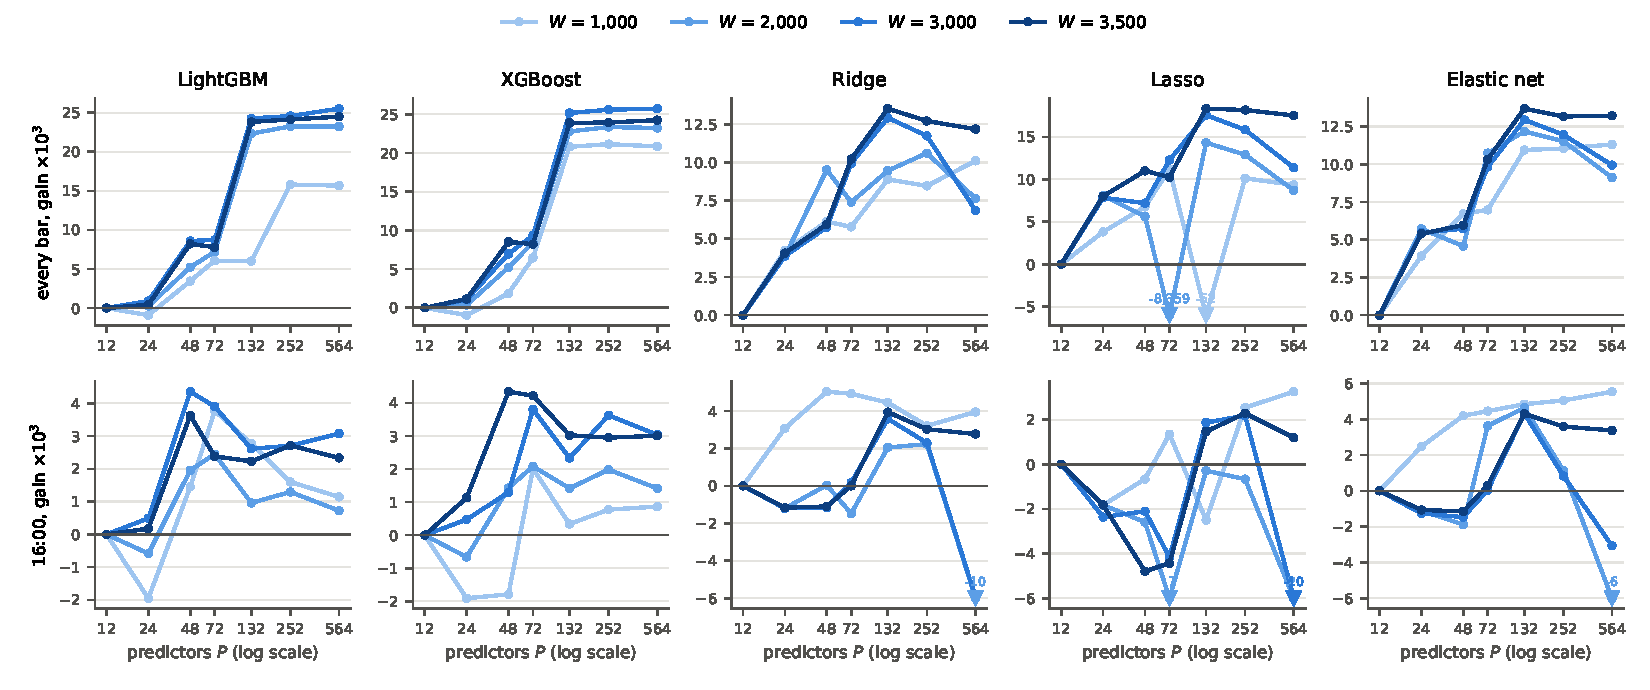
\includegraphics[width=\linewidth]{figures/rehaul_complexity_features.pdf}
  \caption{Feature scaling: the gain over the HAR benchmark set against the number of predictors $P = 12 + 12k$
    ($k = 0, 1, 3, 5, 10, 20, 46$ exogenous series), one line per rolling window ($W = \rhcxWOne$, \rhcxWTwo,
    \rhcxWMain{} and \rhcxWLong{} trading days, $T = 13W$ bars), one panel per model. Gain: QLIKE of the same
    window's $k = 0$ rung minus the rung's, $\times 10^3$, on the \rhcxNBars{} scored bars (top) and the 16:00 bar
    (bottom). Monthly refits at \rhcxNOrigins{} origins. FOMC-patched design.}
  \label{fig:rh_cx_features}
\end{figure}
\begin{figure}[tbp]
  \centering
  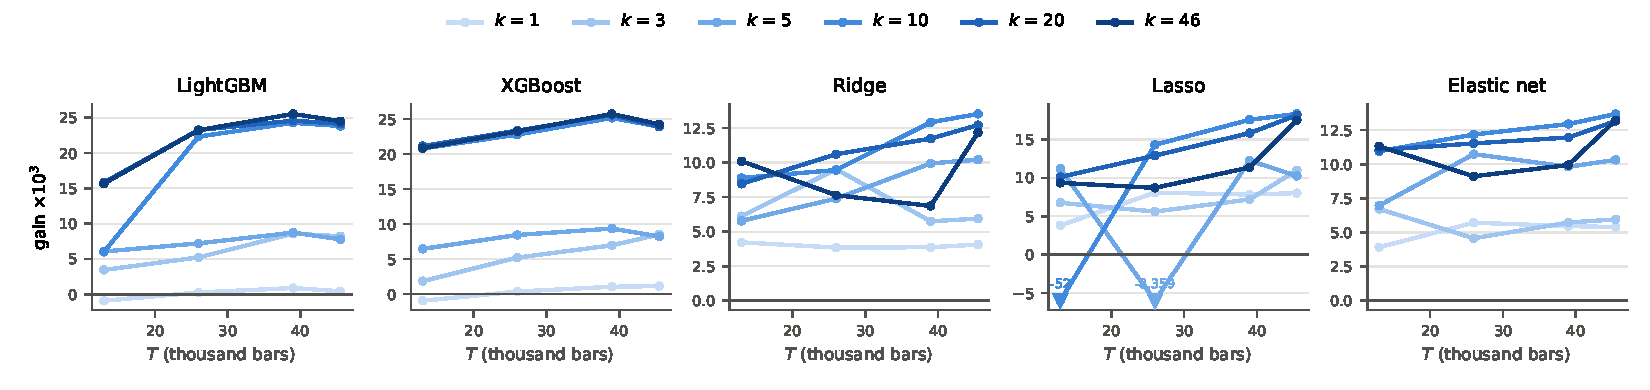
\includegraphics[width=\linewidth]{figures/rehaul_complexity_data.pdf}
  \caption{Data scaling: the gain over the same window's $k = 0$ rung against the window length $T$ at a fixed number
    of exogenous series $k$ (every bar). Same runs as Figure~\ref{fig:rh_cx_features}. FOMC-patched design.}
  \label{fig:rh_cx_data}
\end{figure}

